\documentclass[12pt,Bold,letterpaper,TexShade,twoside]{mcgilletdclass}
\usepackage[dvips,final]{graphicx}
\graphicspath{ {Images/} }
\usepackage[dvips]{geometry}
\usepackage{texshade}
\usepackage{epsf}
\usepackage{epsfig}
\usepackage{bbm}

\usepackage{amsmath}
\usepackage{mathptm}
\usepackage{mathtools}
\usepackage{amssymb}
\usepackage{bm}
\usepackage{tabularx}
\usepackage{tikz}
\usepackage{multirow}

\let\oldemptyset\emptyset
\let\emptyset\varnothing
\DeclareMathOperator{\Tr}{Tr} % trace operator
\newcolumntype{C}[1]{>{\centering\arraybackslash}p{#1}} % centered columns
\newcolumntype{P}[1]{>{\arraybackslash}p{#1}} % left columns

%========================================================%
% \usepackage{adjustbox} % for rotating column headers
% \newcolumntype{R}[2]{%
%     >{\adjustbox{angle=#1,lap=\width-(#2),valign=b}\bgroup}%
%     l%
%     <{\egroup}%
% }
% \newcommand*\rot{\multicolumn{1}{R{-60}{1em}}}
% \newcommand*\rotl{\multicolumn{1}{R{-60}{1em}|}}
%========================================================%

\usepackage{pifont}% http://ctan.org/pkg/pifont
\newcommand{\cmark}{\ding{51}}%
\newcommand{\xmark}{\ding{55}}%
\newcommand{\norm}[1]{\left\lVert#1\right\rVert_2}
\DeclarePairedDelimiter{\ceil}{\lceil}{\rceil}
\DeclarePairedDelimiter{\round}{\lfloor}{\rceil}
\newcommand{\Int}{\int\limits}
\newcommand\Myperm[2][^n]{\prescript{#1\mkern-2.5mu}{}P_{#2}} % permuation notation

%\usepackage{algorithmicx}
%\usepackage{algpseudocode}
%\usepackage{algorithm}
\usepackage{algorithmicx}
\usepackage{algpseudocode}
%\usepackage{algorithm}
\usepackage[linesnumbered,ruled,vlined]{algorithm2e}
\usepackage{url}
\usepackage{multirow}
\usepackage{rotating}
%\usepackage{slashbox}
\usepackage{diagbox}
\usepackage{pgfplots}

\usepackage[symbol]{footmisc} % dagger symbol in footnotes
\renewcommand{\thefootnote}{\fnsymbol{footnote}}

% \usepackage{ragged2e} % left justify text
\usepackage{color, colortbl}
\definecolor{Gray}{gray}{0.9}
\usepackage{xcolor,pgf}
\usepackage[caption=false]{subfig}
%\usepackage[utf8x]{inputenc} 
\usepackage{caption}
%\usepackage{algorithm,algpseudocode,float}
\usepackage{lipsum}
\usepackage{siunitx} % for scientific notation
\usepackage{mathptm}
\usepackage{booktabs}
\usepackage{caption}
\usepackage[french,british]{babel}
\usepackage[square, comma, numbers, compress]{natbib}
\usepackage{doi}
\usepackage{hyperref}
\hypersetup{%
	colorlinks=true,% hyperlinks will be coloured
	linkcolor=blue,% hyperlink text will be blue
	citecolor=blue,% hyperlink text will be blue
	pdfborder = {0 0 0}% no ugly hyperlink border
	pdfborderstyle={/S/U/W 1}% border style will be underline of width 1pt
}

\usepackage{color}
\newcommand{\bl}{\color{blue}}
\newcommand{\rd}{\color{red}}

\usepackage{fancyhdr}
\setlength{\headheight}{15pt}

\pagestyle{fancy}


\fancyhf{}
\fancyhead[LE,RO]{\thepage}
\fancyhead[RE]{{ {{\it \leftmark}}} }
\fancyhead[LO]{{ {\it \rightmark}} }

\fancypagestyle{plain}{ %
	\fancyhf{} % remove everything
	\renewcommand{\headrulewidth}{0pt} % remove lines as well
	\renewcommand{\footrulewidth}{0pt}
}

%========================= ACRONYMS ================================%
\usepackage{acro}
%\acsetup{list-long-format=\capitalisewords}
%\usepackage{mfirstuc}% provides \capitalisewords
\DeclareAcronym{AM}{ short = AM, long = additive manufacturing, short-plural = s, long-plural = s}
\DeclareAcronym{DED}{ short = DED, long = directed energy deposition, short-plural = s, long-plural = s}
\DeclareAcronym{LCA}{ short = LCA, long = life cycle analysis, short-plural = s, long-plural = s}
\DeclareAcronym{MDO}{ short = MDO, long = multidisciplinary design optimization, short-plural = s, long-plural = s}
\DeclareAcronym{FE}{ short = FE, long = finite element, short-plural = s, long-plural = s}
\DeclareAcronym{SN}{ short = SN, long = W{\"o}hler, short-plural = s, long-plural = s}
\DeclareAcronym{CDF}{ short = CDF, long = cumulative probability distribution function, short-plural = s, long-plural = s}
\DeclareAcronym{PDF}{ short = PDF, long = probability density function, short-plural = s, long-plural = s}
\DeclareAcronym{PBD}{ short = PBD, long = point-based design, short-plural = s, long-plural = s}
\DeclareAcronym{CAD}{ short = CAD, long = computer aided design, short-plural = s, long-plural = s}
\DeclareAcronym{CAE}{ short = CAE, long = computer aided engineering, short-plural = s, long-plural = s}
\DeclareAcronym{LH}{ short = LH, long = Latin hypercube, short-plural = s, long-plural = s}
\DeclareAcronym{TRS}{ short = TRS, long = turbine rear structure, short-plural = s, long-plural = s}
\DeclareAcronym{MADS}{ short = MADS, long = mesh adaptive direct search, short-plural = s, long-plural = s}
\DeclareAcronym{OECV}{ short = OECV, long = order error with cross Validation, short-plural = s, long-plural = s}
\DeclareAcronym{OE}{ short = OE, long = order error, short-plural = s, long-plural = s}
\DeclareAcronym{KBN}{ short = KBN, long = kernel-based Bayesian network, short-plural = s, long-plural = s}
\DeclareAcronym{BNC}{ short = BNC, long = Bayesian network classifier, short-plural = s, long-plural = s}
\DeclareAcronym{SBD}{ short = SBD, long = set-based design, short-plural = s, long-plural = s}
\DeclareAcronym{GA}{ short = GA, long = genetic algorithm, short-plural = s, long-plural = s}
\DeclareAcronym{MOP}{ short = MOP, long = multi-objective problem, short-plural = s, long-plural = s}
\DeclareAcronym{OAV}{ short = OAV, long = optimality \& variability, short-plural = s, long-plural = s}
\DeclareAcronym{KDE}{ short = KDE, long = kernel density estimate, short-plural = s, long-plural = s}
\DeclareAcronym{RSM}{ short = RSM, long = response surface methodology, short-plural = s, long-plural = s}
\DeclareAcronym{FDR}{ short = FDR, long = feasible design region, short-plural = s, long-plural = s}
\DeclareAcronym{EDR}{ short = EDR, long = effective design region, short-plural = s, long-plural = s}
\DeclareAcronym{FDS}{ short = FDS, long = feasible design set, short-plural = s, long-plural = s}
\DeclareAcronym{PLM}{ short = PLM, long = product lifecycle management, short-plural = s, long-plural = s}
\DeclareAcronym{DOE}{ short = DOE, long = design of experiments, short-plural = s, long-plural = s}
\DeclareAcronym{LOWESS}{ short = LOWESS, long = locally weighted scatterplot smoothing, short-plural = s, long-plural = s}
\DeclareAcronym{EOL}{ short = EoL, long = end-of-life, short-plural = s, long-plural = s}
\DeclareAcronym{CE}{ short = CE, long = circular economy, short-plural = s, long-plural = s}
\DeclareAcronym{KS}{ short = KS, long = kernel smoothing , short-plural = s, long-plural = s}
\DeclareAcronym{LCC}{ short = LCC, long = lifecyle cost, short-plural = s, long-plural = s}
\DeclareAcronym{CLSC}{ short = CLSC, long = closed-loop supply chain, short-plural = s, long-plural = s}
\DeclareAcronym{SM}{ short = SM, long = surrogate modeling, short-plural = s, long-plural = s}
\DeclareAcronym{POA}{ short = POA, long = post-optimality analysis, short-plural = s, long-plural = s}
\DeclareAcronym{DFRem}{ short = DFRem, long = design for remanufacturing, short-plural = s, long-plural = s}
\DeclareAcronym{CP}{ short = CP, long = constraint programming, short-plural = s, long-plural = s}
\DeclareAcronym{PRS}{ short = PRS, long = polynomial response surface, short-plural = s, long-plural = s}
\DeclareAcronym{FEA}{ short = FEA, long = finite element analysis, short-plural = s, long-plural = s}
\DeclareAcronym{OEM}{ short = OEM, long = original equipment manufacturer, short-plural = s, long-plural = s}
\DeclareAcronym{TSE}{ short = TSE, long = tradespace exploration, short-plural = s, long-plural = s}
\DeclareAcronym{FO}{ short = FO, long = filtered outdegree, short-plural = s, long-plural = s}
\DeclareAcronym{DFO}{ short = FO, long = derivative-free optimization, short-plural = s, long-plural = s}
\DeclareAcronym{NM}{ short = NM, long = Nelder-Mead, short-plural = s, long-plural = s}
\DeclareAcronym{GPS}{ short = GPS, long = generalised pattern search, short-plural = s, long-plural = s}
\DeclareAcronym{CS}{ short = CS, long = coordinate search, short-plural = s, long-plural = s}
\DeclareAcronym{RBDO}{ short = RBDO, long = reliability-based design optimization, short-plural = s, long-plural = s}
\DeclareAcronym{MPP}{ short = MPP, long = most probable point, short-plural = s, long-plural = s}
\DeclareAcronym{MCS}{ short = MCS, long = Monte Carlo simulation, short-plural = s, long-plural = s}
%=================================================================%

%\usepackage{natbib}
%\usepackage[square, comma, numbers, sort&compress]{natbib}
%\bibliographystyle{unsrtnat}

\makeatletter
\def\hlinewd#1{%
	\noalign{\ifnum0=`}\fi\hrule \@height #1 %
	\futurelet\reserved@a\@xhline}
%\bibliographystyle{unsrtnat}
\setlength{\parskip}{0pt}
%\usepackage{tex4ht}
%\usepackage{amsmath}
%%%%%%%%%%%%%%%%%%%%%%%%%%%%%%%%%%%%%%%%%%%%%%%%%%%%%
%% Have you configured your TeX system for proper  %%
%% page alignment? See the McGillETD documentation %%
%% for two methods that can be used to control     %%
%% page alignment. One method is demonstrated      %%
%% below. See documentation and the ufalign.tex    %%
%% file for instructions on how to adjust these    %%
%% parameters.                                     %%
%%                                                 %%
%%%%%%%%%%%%%%%%%%%%%%%%%%%%%%%%%%%%%%%%%%%%%%%%%%%%%
%%       Define student-specific info
\SetTitle{\huge{Optimization-driven set-based design for dynamic design requirements}}%
\SetAuthor{Khalil Al Handawi}%
\SetDegreeType{Doctor of Philosophy}%
\SetDepartment{Department of Mechanical Engineering}%
\SetUniversity{McGill University}%
\SetUniversityAddr{Montreal, Quebec}%
\SetThesisDate{\today}%
\SetRequirements{A thesis submitted to McGill University in partial fulfilment of the requirements of
	the degree of Doctor of Philosophy}%
\SetCopyright{\copyright~Khalil Al Handawi 2020
}%

%\makeindex[keylist]
%\makeindex[abbr]

%% Input any special commands below
%\newcommand{\Kron}[1]{\ensuremath{\delta_{K}\left(#1\right)}}
\listfiles%
\begin{document}

\maketitle%

\begin{romanPagenumber}{2}%

%%%%%%%%%%%%%%%%%%%%%%%%%%%%%%%%%%%%%%%%%%%%%%%%%%%%%
%%                  Dedication                     %%
%%%%%%%%%%%%%%%%%%%%%%%%%%%%%%%%%%%%%%%%%%%%%%%%%%%%%
\SetDedicationName{Dedication}%
\SetDedicationText{\centering My effort, I dedicate to my sweet and loving \\ 
	\textit{mother, father, and sister},\\
	whose love, encouragement, and prays of day and night make me able to attain the highest and most honorable of professions.}%
\Dedication%

%%%%%%%%%%%%%%%%%%%%%%%%%%%%%%%%%%%%%%%%%%%%%%%%%%%%%
%%                Acknowledgments                  %%
%%%%%%%%%%%%%%%%%%%%%%%%%%%%%%%%%%%%%%%%%%%%%%%%%%%%%
\SetAcknowledgeName{Acknowledgements}%
\SetAcknowledgeText{I would like to thank my supervisor, Prof. Michael Kokkolaras, for providing me with the opportunity and limitless freedom to innovate and pursue my research interests. He was an invaluable resource and mentor that has molded me into a professional and adept researcher and engineer. He always stressed the importance of quality research and responsible academic practices making them a part of my identity as a researcher. He made me realize my full potential and capabilities through his encouragement and vision. Thank you for being available even outside of office hours and providing me with access to knowledge and resources that is unprecedented in all my years of education.\\
%
I also wish to thank my committee members Prof. Damiano Pasini and Prof. Mathias Legrand for their advice and guidance throughout my graduate studies at McGill University.\\
%
I would like to express my most profound appreciation to my collaborators at Chalmers University of Technology at Gothenburg, Sweden for providing me with the resources and connections to contextualize my contributions and better bring them to the engineering design community. I wish to particularly thank Prof. Ola Isaksson and Dr. Massimo Panarotto for their constant guidance and suggestions for improving the relevance of my work to the industry in which it will be applied.\\
%
I am very grateful to GKN Aerospace, Engine Systems at Trollh\"{a}ttan, Sweden for giving me the opportunity to implement my work on challenging engineering applications. I wish to thank Dr. Petter Andersson for his steadfast support, advice, and guidance throughout my work.\\
%
I am grateful for the partial support of this work by grants NSERC CRDPJ 479630-15 X-243027 and CARIC CRDPJ479630-15 X-243067. I am also very grateful for the partial support of FRQNT through the {\em Bourses de doctorat en recherche} program (file 273486). I am grateful to the Faculty of Engineering at McGill University for its partial support through a McGill Engineering Doctoral Award.\\
%
To my mother Chaza, thank you for your persistent encouragement and support. Your belief in me and my abilities propels me ever further in my educational journey. To my father Bassam, thank you for everything you gave and taught me and for instilling a sense of curiosity and love for discovery and learning ever since I was a child by taking me to your chemistry lab. To my sister Marieh, thank you for your continuous steady support. Whenever I fall, I always find you by my side helping me to stand back up again. I would like to acknowledge my pet cat Daboos for his emotional support that meant a lot to me. I hope you are in a better place now.\\
%
Finally, I would like to show appreciation for my fellow graduate students at McGill for making this a memorable experience. We have forged lifelong friendships through the experiences we shared.
}%
\Acknowledge%

%%%%%%%%%%%%%%%%%%%%%%%%%%%%%%%%%%%%%%%%%%%%%%%%%%%%%
%%                 Contributions                   %%
%%%%%%%%%%%%%%%%%%%%%%%%%%%%%%%%%%%%%%%%%%%%%%%%%%%%%
\SetContributionName{Contributions to original knowledge}%
\SetContributionText{The thesis presents a number of design frameworks for addressing uncertain and dynamic design requirements. They are listed as follows.
%
\begin{enumerate}
	\item{A \acl{SBD} framework for identifying sets of parametric optimal designs and scalable optimal designs.}\\
	%
	The following metrics and algorithms were developed as part of this framework.
	%
	\begin{enumerate}
		\item{A surrogate-enabled parametric optimization scheme using derivative-free methods for obtaining parametric optimal designs.}
		\item{A response surface methodology for performing post-optimality analysis on the parametric optimal designs and evaluating their scalability.}
		\item{A scalability constraint formulated in the parameter space.}
		\item{A methodology for mapping scalable optimal designs from the parameter space to the design space using random sampling techniques.}
	\end{enumerate}
	%
	\item{A design margin quantification and allocation tool for addressing changing requirements throughout a product's lifecycle or development process.}\\
	%
	The following metrics and algorithms were developed as part of this framework.
	%
	\begin{enumerate}
		\item{A method for computing reliability and excess of a particular design and requirement using Monte Carlo integration.}
		\item{A method for generating different product development or lifecycle scenarios using Monte Carlo simulation and importance sampling.}
		\item{A set-based decision making approach for obtaining sets of optimal design decisions.}
		\item{A \acl{SBD} method for obtaining flexible and robust sets of solutions.}
		\item{A tradespace exploration strategy for visualizing and comparing flexible, robust and optimal sets of solutions.}
	\end{enumerate}
\end{enumerate}
%
\textbf{Contribution of Authors}\\
%
The author of this thesis is the sole contributor to the entire material of each chapter presented in this thesis; he has developed all of the ideas and their implementation under the guidance of his supervisor.\\
%
Some of the material presented in this thesis has appeared in conference and journal papers that include additional co-authors who contributed to discussion and exchange of ideas (during the author's summer visit stays at Chalmers University of Technology and collaboration with GKN Aerospace Engine Systems Sweden), review of manuscript drafts, and practical interpretation of case study results. None of the material presented in this thesis has been developed by any of these co-authors.
}%
\Contribution%

%%%%%%%%%%%%%%%%%%%%%%%%%%%%%%%%%%%%%%%%%%%%%%%%%%%%%
%%                English Abstract                 %%
%%%%%%%%%%%%%%%%%%%%%%%%%%%%%%%%%%%%%%%%%%%%%%%%%%%%%
\SetAbstractEnName{Abstract}%
\SetAbstractEnText{This thesis presents novel design methodologies for obtaining a set of design solutions to address design requirements that may change during the design process or over a product or system’s lifetime. These methodologies aim at supporting design engineers quantitatively so they can make informed decisions in the early phases of product development when uncertainty is high.
The presented methodologies consider design problems commonly encountered in industry. The applications used in this thesis demonstrate the efficacy of these methodologies and are centered around product remanufacturing by means of directed energy deposition, an additive manufacturing technique. Specifically, they aim at providing design solutions in the form of geometry of the deposit and the remanufacturing process parameters. 
The first methodology considers remanufacturing as a strategy to address changing requirements in design problems. Sets of optimal design solutions, as opposed to single-point designs, are obtained using numerical optimization. The optimization problem objective is to maximize structural performance subject to design and process constraints. Since optimality and feasibility depend on varying design parameters, parametric studies are conducted to obtain optimal solutions for different parameter values. A response surface of the optimization solutions captures the effect of changing one or more parameters on the optimal solution and provides a method to map designs from the design space to the parameter space. A manufacturing transition rule is formulated in the parameter space to identify sets of design solutions that are scalable by additive manufacturing. The transition rule is based on the physical limitations of the manufacturing method. Scalable design solutions are mapped back to the design space to obtain the corresponding design variable values. This methodology draws inspiration from set-based design principles used to generate sets of design solutions rather than converging to a single design solution early in the product development process. 
The first methodology focuses on making decisions using information that is available to the designer. Since product development involves several design iterations and stages, a second methodology for making decisions based on information from past iterations is introduced in this thesis. It focuses on additive manufacturing problems where design requirements remain constant throughout a time interval referred to as an epoch and only change at discrete times in between epochs. This results in a series of design decisions that must be made at the end of each epoch referred to as a decision arc. This methodology considers selecting the best combination of design decisions from a set of discrete design choices. A combinatorial optimization problem is formulated to minimize the level of overdesign subject to reliability constraints. The reliability constraints are computed by evaluating the probability that a design will satisfy a design requirement given by a joint probability density function. Several design requirements are chained together and defined at the end of each epoch to form a requirement arc. Several requirement arc samples are generated using importance sampling. The combinatorial optimization problem is solved for each requirement arc to obtain a set of corresponding decision arcs. This set of optimal decision arcs is compared against sets of robust and flexible design arcs. A tradespace is used to visualize the design sets and identify the relative degree of flexibility and robustness in the set of optimal decision arcs.
The remanufacturing of a turbine rear structure, an aeroengine structural component is used to test the proposed methodologies. A stiffener is deposited on the outer casing of the turbine rear structure to increase its stiffness when subjected to thermal loads due to the exhaust gases. The first methodology is used to determine the sets of optimal and scalable stiffener designs by optimizing the geometry and laser power used to deposit the stiffener. The second methodology is used to identify the set of optimal design arcs by chaining together several discrete stiffener designs to minimize the overall level of overdesign while maintaining a threshold reliability throughout the design process or the product’s lifecycle.
The two methodologies form a complete set-based design paradigm for addressing changing requirements in design problems featuring continuous and discrete design variables for instantaneous or progressive change in the design requirements.}
\AbstractEn%

%%%%%%%%%%%%%%%%%%%%%%%%%%%%%%%%%%%%%%%%%%%%%%%%%%%%%
%%                French Abstract                  %%
%%%%%%%%%%%%%%%%%%%%%%%%%%%%%%%%%%%%%%%%%%%%%%%%%%%%%
\begin{otherlanguage}{french} 
\SetAbstractFrName{ABR\'{E}G\'{E}}%
\SetAbstractFrText{Cette thèse présente de nouvelles méthodologies de conception pour obtenir un ensemble de solutions de conception qui peuvent répondre aux exigences de conception qui peuvent changer au cours du processus de conception ou au cours de la durée de vie d'un produit ou d'un système. Ces méthodologies visent à aider les ingénieurs de conception quantitativement afin qu'ils puissent prendre des décisions éclairées dans les premières phases du développement de produits lorsque l'incertitude est élevée.
Les méthodologies présentées prennent en compte les problèmes de conception couramment rencontrés dans l'industrie. Les applications utilisées dans cette thèse démon\allowbreak trent l'efficacité de ces méthodo-\allowbreak logies et sont centrées sur la refabrication de produits par dépôt d'énergie dirigé, une technique de fabrication additive. Plus précisément, ils visent à fournir des solutions de conception sous la forme de la géométrie du gisement et des paramètres du processus de reconditionnement.
La première méthodologie considère le reconditionnement comme une stratégie pour répondre aux exigences changeantes des problèmes de conception. Des ensembles de solutions de conception optimales, par opposition aux conceptions à un seul point, sont obtenus à l'aide de l'optimisation numérique. L'objectif du problème d'optimisation est de maximiser les performances structurelles soumises aux contraintes de conception et de processus. Étant donné que l'optimalité et la faisabilité dépendent de paramètres de conception variables, des études paramétriques sont menées pour obtenir des solutions optimales pour différentes valeurs de paramètres. Une surface de réponse des solutions d'optimisation capture l'effet de la modification d'un ou plusieurs paramètres sur la solution optimale et fournit une méthode pour mapper des conceptions de l'espace de conception à l'espace de paramètres. Dans l'espace des paramètres, une règle de transition de fabrication est formulée pour identifier des ensembles de solutions de conception qui sont évolutives par fabrication additive. La règle de transition est basée sur les limites physiques de la méthode de fabrication. Les solutions de conception évolutives sont ensuite mappées vers l'espace de conception pour obtenir les valeurs des variables de conception correspondantes. Cette méthodologie s'inspire des principes de conception basés sur des ensembles utilisés pour générer des ensembles de solutions de conception plutôt que de converger vers une solution de conception unique au début du processus de développement du produit.
La première méthodologie se concentre sur la prise de décisions en utilisant les informations dont dispose le concepteur. Étant donné que le développement de produits implique plusieurs itérations et étapes de conception, une deuxième méthodologie pour prendre des décisions basées sur les informations des itérations passées est introduite dans cette thèse. Il se concentre sur les problèmes de fabrication additive où les exigences de conception restent constantes tout au long d'un intervalle de temps appelé époque et ne changent qu'à des moments discrets entre les époques. Il en résulte une série de décisions de conception qui doivent être prises à la fin de chaque époque, appelées arc de décision. Cette méthodologie considère la sélection de la meilleure combinaison de décisions de conception à partir d'un ensemble de choix de conception discrets. Un problème d'optimisation combinatoire est formulé pour minimiser le niveau de sur-conception soumis à des contraintes de fiabilité. Les contraintes de fiabilité sont calculées en évaluant la probabilité qu'une conception satisfasse à une exigence de conception donnée par une fonction de densité de probabilité conjointe. Plusieurs exigences de conception sont enchaînées et définies à la fin de chaque époque pour former un arc d'exigences. Plusieurs échantillons d'arc d'exigence sont générés en utilisant un échanti\-llonnage d'importance. Le problème d'optimisation combinatoire est résolu pour chaque arc d'exi\-gence pour obtenir un ensemble d'arcs de décision correspondants. Cet ensemble d'arcs de décision optimaux est comparé à des ensembles d'arcs de conception robustes et flexibles. Un espace commercial est utilisé pour visualiser les ensembles de conception et identifier le degré relatif de flexibilité et de robustesse dans l'ensemble des arcs de décision optimaux.
La remise à neuf d'une structure arrière de turbine, un composant structurel de moteur d'avion est utilisé pour tester les méthodologies proposées. Un raidisseur est déposé sur le carter extérieur de la structure arrière de la turbine pour augmenter sa rigidité lorsqu'elle est soumise à des charges thermiques dues aux gaz d'échappement. La première méthodologie est utilisée pour déterminer l'ensemble des conceptions optimales de raidisseurs et l'ensemble des conceptions de raidisseurs évolutifs en optimisant la géométrie et la puissance laser utilisées pour déposer le raidisseur. La deuxième méthodologie est utilisée pour identifier l’ensemble des arcs de conception optimaux en enchaînant plusieurs conceptions de raidisseurs discrets pour minimiser le niveau global de sur-conception tout en maintenant un seuil de fiabilité tout au long du processus de conception ou du cycle de vie du produit.
Les deux méthodologies forment un paradigme de conception basé sur un ensemble complet pour répondre aux exigences changeantes dans les problèmes de conception comportant des variables de conception continues et discrètes pour un changement instantané ou progressif des exigences de conception.}%
\AbstractFr%
\end{otherlanguage}
\TOCHeading{Table of Contents}%
\LOTHeading{List of Tables}%
\LOFHeading{List of Figures}%
\tableofcontents %
\listoftables %
\listoffigures %

\end{romanPagenumber}

%\mainmatter %

% Chapter 01: Introduction
%%%%%%%%%%%%%%%%%%%%%%%%%%%%%%%%%%%%%%%%%%%%%%%%%%%%%%%
%%                   Introduction                    %%
%%%%%%%%%%%%%%%%%%%%%%%%%%%%%%%%%%%%%%%%%%%%%%%%%%%%%%%
\chapter{Introduction}
\chaptermark{Introduction}
\label{ch:intro}
%%%%%%%%%%%%%%%%%%%%%%%%%%%%%%%%%%%%%%%%%%%%%%%%%%%%%%%

The development of aerospace systems relies on the definition and communication of design requirements from the stakeholders to the \acp{OEM}, who then define and communicate design requirements to the suppliers of components. In this context, design requirements specify for each manufacturing organization what the components shall achieve in order to provide value to stakeholders once integrated as part of a system \cite{Blanchard1981}. While requirements are supposed to be clear and well-defined, they are subject to changes during a development project \cite{Peterson2007}. Due to the large number of stakeholders and design teams involved in the design of complex products, requirements are in constant flux even after a product has been commissioned. 

We consider the aerospace industry as an example. Requirement changes occur for a plethora of reasons \cite{Boeing2013,Eckert2004}. The temperature loads a structural component must sustain in operation may change during product development due to a shift in the engine architecture specified by the engine \ac{OEM}. Furthermore, requirements may change during the in-service phase due to changes in the market or in the legislation that governs the industry. There is an inherent uncertainty in design requirements at the beginning of a product development project, which gradually decreases as the project advances and decisions are made. At the beginning, where the innovation potential is high, such uncertainty can be very large \cite{ullman2009mechanical}. In the early phases, design requirements are normally communicated as ranges, and the final requirement (e.g. temperature load) may lie anywhere in this range (or in some cases, even outside).

If the product's specifications fall short of the requirements during development or product lifecycle, an upgrade to the specifications is warranted to maintain functionality. This may involve a complete redesign of the product depending on the severity of the required changes. Complete redesign involves discarding the current iteration of the product and starting a new development cycle with the changed requirements as inputs. This cradle-to-grave approach is extremely inefficient when considering a \ac{CE} where value is generated from each unit of resource by recovering and regenerating products and materials at the end of each service life \cite{MacArthur2013b}. In order to increase the recoverability of the product, and avoid loss in value due to disposal, products should be designed for such activities in order to increase their relevance in a \ac{CE} and extract as much value from them as possible. Recovering a product involves returning its specifications to its pre-disposal levels. However, requirements are seldom the same after a product's lifecycle has run its course. As a result, the product's specifications have to be upgraded to meet the set of requirements expected of current generation products. Designing products for such unforeseeable requirements is the main subject of this thesis.

This thesis utilizes numerical methods for addressing the problem of designing prod\-ucts for remanufacturing activities where requirements are expected to be highly dynamic. In this chapter, Section \ref{sec:motivation} provides motivation for implementing the design para\-digms introduced in this thesis to mitigate the challenges that arise due to changing product requirements. The research objectives of this thesis are then discussed in the context of product remanufacturing design problems. The contributions of this thesis to the field of engineering design for uncertain requirements are then outlined in Section~\ref{sec:contribution}. The chapter concludes by outlining the remainder of the thesis in Section \ref{sec:outline}.

%============================= MOTIVATION ==============================%
\section{Motivation}
\label{sec:motivation}

The increasing environmental impact of industrial activities is changing the perception of legislators and business enterprises towards the importance of recovering value from products that have reached the end of their useful lifecycles, especially if this end is brought about by an unforeseen change in requirements or specifications. As a result, a new paradigm for product design has become increasingly relevant in modern economies.

%---------------------------------------------------------------------%
% Circular economy
\subsection{Circular economy and product recovery} \label{subsec:CE}

A \ac{CE} can be used to return products that have reached the end of their useful lifecycles into service and extract as much value from them as possible. \ac{CE} helps achieve both economic growth and environmental protection. Since resources are limited, legislation has been put forth so that business enterprises bear responsibility for the environmental, social and economic impacts their products have on society \cite{Matos2007}. This caused business enterprises to adopt sustainable development practices when designing their products.

A \ac{CLSC} can return used or discarded products to working condition. This enables sustainable development by reducing the environmental impact of products \cite{QuariguasiFrotaNeto2010}. A \ac{CLSC} includes a forward supply chain where products are used normally until the end of their life and a reverse supply chain that returns the discarded products to a previous stage in its lifecycle. Examples of recovery activities in a reverse supply chain include remanufacturing, reuse and recycling \cite{Lieder2016,MacArthur2013a}. Since \ac{CE} encompasses products as well as their forward and reverse supply chains, businesses must design their products for closed-loop product recovery activities \cite{Lieder2016}. This includes design for remanufacturing, recycling and reuse. In this thesis, we focus on remanufacturing since it is more sustainable than recycling and recovers more value across the supply chain due to increased virgin material substitution and retention of the embodied energy used to manufacture the original product from the raw materials \cite{MacArthur2013a,Goodall2014}. 

There is a number of studies that consider product design for remanufacturing \cite{Ijomah2010,Liu2017}. However, the majority focus on closed-loop supply chain logistics of remanufacturing \cite{Mahadevan,Golinska2015,VanThao2015,Song2005,Koren2018}. Product remanufacturing design problems are more challenging to address due to the variable design requirements encountered during product design. Studies that focus on remanufacturing design are reviewed in Section \ref{sec:remanufacturingdesign}. 

Design for remanufacturing rules found in the literature specify that a product's components should allow room for modifications to meet design requirements \cite{Ijomah2009}. Furthermore, it is important to distinguish refurbishment from remanufacturing: the former is used to satisfy original specifications, whereas the latter allows for considering changed requirements. As a result, products should be designed for changing requirements to enable product recovery by remanufacturing.

%---------------------------------------------------------------------%
% Design for changing requirements
\subsection{Designing for changing requirements} \label{subsec:changingreq}

Design requirements are subject to change during a product's lifecycle \cite{Goodall2014,Lindahl2007,Thierry2012,American2017}. Variable parameters such as customer requirements and loading conditions influence des\-ign requirements such as cost and product life requirements \cite{Fricke2005} and can be unpredictable despite the best efforts of forecasters and analysts \cite{DeNeufville2011}.

Design \textit{changeability} enables designs to change through a number of change mechanisms whose aspects can include flexibility, agility, robustness, and adaptability. A number of basic and extended principles have been identified as enablers of design changeability \cite{Fricke2005}. In this thesis we focus on two aspects of changeability, flexibility and robustness in product design for accommodating uncertain requirements. Advances in incorporating design changeability in product design are reviewed in Section~\ref{sec:changeability}.

The first contribution of this thesis provides a rigorous formulation for flexibility in terms of \textit{scalability}. Scalability is an aspect of flexibility which is defined in the literature and expanded upon in Section \ref{sec:changeability}. Scalability is highly relevant to remanufacturing design problems as will be explained in Chapter~\ref{ch:background}. Decisions regarding the scalability of a remanufacturing design are made based on current information that is available to the designer. The issue of designing a product based on the current state of the product and its corresponding requirements has been addressed by \citeauthor{Alhandawi2020} \cite{Alhandawi2020}.

However, requirements change over the course of a product development project or life\-cycle. A decision-making tool based on past and current information is required \cite{Eckert2019}. The second contribution of this thesis formulates and quantifies design flexibility and robustness over the course of a remanufacturing design process. Decisions about the desired amount of flexibility and robustness are made based on current and past information from the design process or the product lifecycle.

The motivation for such a decision-making tool stems from conventional design practices with regards to changing requirements. We use a thought experiment to provide motivation for the research presented in this thesis.

%---------------------------------------------------------------------%
% Motivation problem
\subsection{A thought experiment} \label{subsec:thoughtexperiment}

Designers address changing requirements using different design strategies. One strat\-egy involves frequent redesign of the component as system requirements are constantly updated and cascaded down to the component level \cite{Eckert2004}. This is an example of \textit{flexible} design. Another strategy for managing change is by building design \textit{margins} into the component such that it incorporates a buffer against change \cite{Clarkson2004,Eckert2004}. Several researchers have developed metrics for these quantities which are reviewed in Section~\ref{sec:margins}. This buffer helps reduce the amount of redesign needed to satisfy an uncertain set of requirements by \textit{absorbing} change. This is an example of a \textit{robust} design. Flexibility and robustness are two ends of a spectrum in terms of design changeability and balance between the two can help mitigate unnecessary overdesign. Let us consider a problem from the industry and explore our options for tackling it.

\begin{figure}[h!]
	\centering
	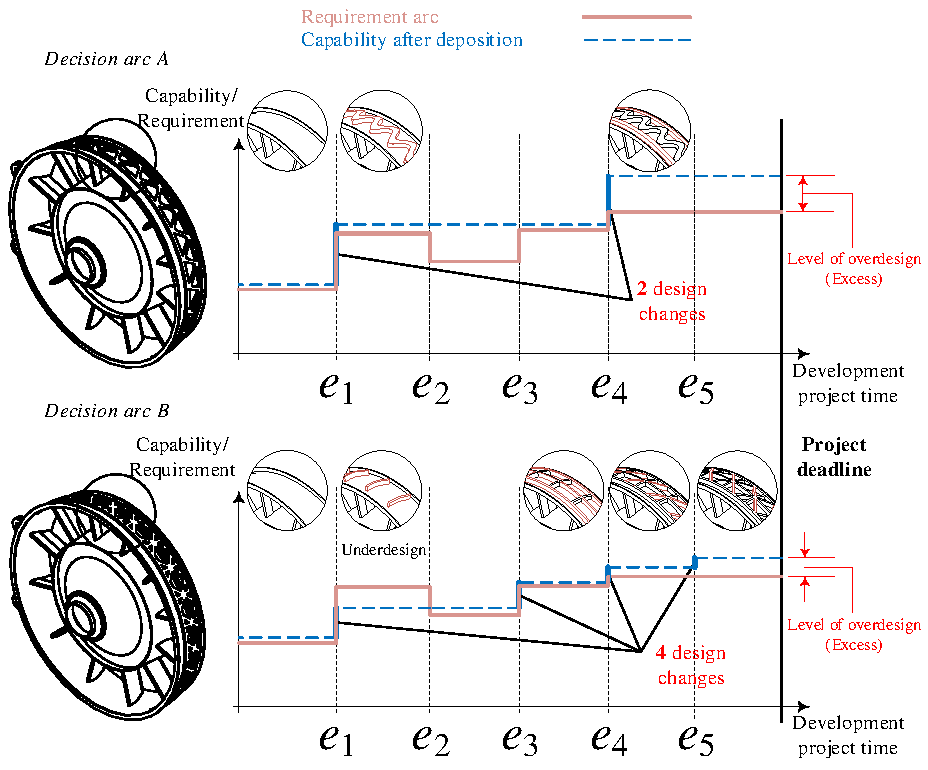
\includegraphics[width=0.9\textwidth]{problem_description.pdf}
	\caption{Example product development project showcasing different decision arcs}
	\label{fig:problemdescription}
\end{figure}

A \acf{TRS} (a static structural component in an aeroengine) must sustain temperature loads as a result of the hot engine exhaust gases. These temperature loads can change during the course of a development project or during the in-service phases. In Figure~\ref{fig:problemdescription}, these changes are represented by the “requirement arc” (red line). For simplicity, in this example the temperature requirement is assumed to change five times, in conjunction with critical design reviews \cite{Cooper2008}. The period of time in which a requirement is held constant is referred to as an \textit{epoch} \cite{McManus2007}. The benefit of using \ac{AM} for remanufacturing the \ac{TRS} is exemplified by two decision \textit{arc}s A and B. The terms epoch and arc are expanded upon in Chapter~\ref{ch:TSEcont}. With \ac{AM}, the geometry of the \ac{TRS} can be initially designed ($e_1$) to meet the lower bound of the temperature range, while depositing a stiffener on the structure as the temperature requirement changes. This strategy resonates well with flexible design principles, which suggest designing for a relatively low capability that can be expanded if changes occur \cite{DeNeufville2011}. However, the decisions made during the design of the stiffener’s geometry may impact such flexibility substantially. For instance, choosing the deposit geometry given by decision arc A at $e_2$ (wavy design concept) will result in a design with a capacity that fulfils the new requirement. However, further changes of this geometry (such as the one made at $e_4$) do not allow for close tracking of the requirement arc, resulting in overdesign (the blue line in Figure~\ref{fig:problemdescription}). On the other hand, decision arc B (hatched design concept) allows for a better tracking of the requirement arc. This reduces the risk for overdesign at the end of the project. However, this comes with the cost and effort of performing more depositions during the course of the development (4 instead of 2) which are costly and time consuming, outweighing the benefits given by this more flexible decision arc. Furthermore, the capability is lower than the requirement in some cases which may not always be acceptable during a development project.

This example draws inspiration from the contrast in longevity of the B-52 stratofortress bomber and F/A-18 hornet. The B-52 enjoyed a longer service cycle and was able to cope with the needed modifications due to technological advancements as opposed to the F/A-18 hornet. This was due to the embedded design margins (in the form of excess) during initial production of the B-52. The F/A-18 hornet had more \textit{modularity} (a form of flexibility) to counteract the reduced margins available for upgrade but still suffered greatly once the margins were consumed during its service life requiring a complete redesign \cite{Long2017}. This case study underscores the necessity for quantifying and strategically allocating design margins in product design.

We aim to address the shortcomings of either design strategy that were identified in this thought experiment. We formulate the thesis objectives accordingly.

%---------------------------------------------------------------------%
% Thesis objectives
\subsection{Objectives} \label{subsec:objectives}

% Furthermore, there is a trade-off between the flexibility that can be enabled by \ac{AM} and other attributes of the design (such as weight, manufacturing costs and excess) that need to be optimized in the early design phases. We review a number of studies that utilize tradespace exploration strategies so that the tradeoff between product costs and its degree of flexibility or robustness as given by the metrics developed in this thesis can be studied. These studies are summarized in Section~\ref{sec:tradespace}.

% Arguably, a set of changeable solutions is required to leverage the added design changeability in order to provide possible alternative designs. \Acf{SBD} is a design paradigm that places emphasis on a varied solution set as a means for accommodating uncertain requirements. Consequently, results from both contributions of this thesis are presented as sets of design solutions by employing the principles of \ac{SBD}. Feasibility of the solutions with respect to the requirements and changeability must be checked and maintained throughout the solution set. Advances in \ac{SBD} are reviewed in Section~\ref{sec:SBD}.

% Having explained the rationale behind the scope and motivation of this thesis, we outline the objectives and contributions in the following section.

The goal of this thesis is to develop several design frameworks for managing uncertain design requirements during the product development process or throughout its lifecycle. 

The frameworks developed in this thesis follow the principles of \acf{SBD} by providing a set of feasible design solutions in order to leverage the added design changeability from our frameworks. 

Feasibility is assessed using engineering models which can be computationally intensive. Specifically, remanufacturing design problems involving \ac{AM} feature thermomechanical models with coupled thermal and structural analyses of the deposition process. These thermomechanical models are developed for the \ac{TRS} described earlier as it will be used as a remanufacturing design problem to demonstrate our methods. The thermomechanical models are evaluated prior to assessing the feasibility of the design in terms of its structural performance. In order to navigate the design space with relative ease in search of the solution sets respective of each framework, a surrogate model is obtained by training a response surface model with data obtained from the thermomechanical/engineering model.

Decisions are rendered in each framework using rigorous derivative-free optimization algorithms. This is due to the non-smooth response that can be exhibited by the thermomechanical/engineering models and their surrogates.

The first framework provides decisions about the design variables in order to maintain scalability in the set of design solutions given current information about the state of the design problem. Parametric design optimization is used to assess feasibility while maximizing structural performance to obtain a set of parametric optimal designs in the design space. A response surface of the optimization solutions with respect to the parameters governing the design requirements is constructed in the parameters space. A scalability constraint based on the manufacturing process used is formulated in the parameters space and used to identify scalable design solutions that can be mapped back to the design space.

The second design framework provides decisions regarding design variables such that overdesign (excess) is minimized throughout the different stages of the development process or the product lifecycle while maintaining a threshold reliability level with respect to uncertain requirements. Monte Carlo integration is used at each stage where decisions are made to quantify the reliability (probability of satisfying a requirement governed by a joint probability density function) and excess. Additionally, metrics for quantifying flexibility and robustness are developed as part of this framework. Monte Carlo simulation is used to generate and chain together different requirements. Corresponding design decisions are obtained by solving a combinatorial optimization problem. This results in sets of optimal, flexible, and robust design solutions. The effect of minimizing excess on robustness and flexibility is investigated via tradespace exploration.

The objectives are summarized as follows.

\begin{itemize}
	\item{Develop a framework for identifying design solutions that have the greatest potential for remanufacturing.}
	\item{Strategically quantify and allocate the aspects of design flexibility and robustness to address changing requirements during remanufacturing.}
	\item{Provide a sufficiently diverse set of equally reamnufacturable solutions to provide designers with alternatives after committing to a particular solution.}
\end{itemize}

% \begin{itemize}
% 	\item{Utilize the principles of \ac{SBD} to obtain sets of design solutions}
% 	\item{Utilize rigorous derivative-free optimization algorithms since we use engineering models that are prone to nonsmooth responses}
% 	\item{Use parametric design optimization to obtain a set of feasible design solutions for an instance during the product development process or during its lifecycle}
% 	\item{Use response surface of parametric optimization solutions to map between design and parameters spaces}
% 	\item{Formulate and use a scalability constraint in the parameters space to identify scalable optimal designs}
% 	\item{Compute instantaneous reliability and excess for a particular design and requirement at a certain stage in its product development process or lifecycle}
% 	\item {Minimize cumulative excess throughout product development process or lifecycle to mitigate overdesign}
% 	\item{Obtain sets of optimal, flexible and robust design solutions corresponding to different product development or lifecycle scenarios}
% \end{itemize}
%=========================== CONTRIBUTIONS =============================%
%============================= MOTIVATION ==============================%
\section{Contributions}
\label{sec:contribution}

The contributions of this thesis are as follows.

\begin{enumerate}
	\item{An \ac{SBD} framework for identifying sets of parametric optimal designs and scalable optimal designs.}
	
	The following metrics and algorithms were developed as part of this framework.
	
	\begin{enumerate}
		\item{A surrogate enabled parametric optimization scheme using derivative free methods for obtaining parametric optimal designs.}
		\item{A response surface methodology for performing post optimality analysis on the parametric optimal designs and evaluating their scalability.}
		\item{A scalability constraint formulated in the parameters space}
		\item{A methodology for mapping scalable optimal designs from the parameters space to the design space using random sampling techniques.}
	\end{enumerate}
	%
	\item{A design margin quantification and allocation tool for addressing changing requirements throughout a product's lifecycle or development process.}
	
	The following metrics and algorithms were developed as part of this framework.
	
	\begin{enumerate}
		\item{A method for computing reliability and excess of a particular design and requirement using Monte Carlo integration.}
		\item{A method for generating different product development or lifecycle scenarios using Monte Carlo simulation and importance sampling.}
		\item{An \ac{SBD} combinatorial optimization approach for obtaining sets of optimal designs.}
		\item{An \ac{SBD} method for obtaining flexible and robust sets of solutions.}
		\item{A tradespace exploration strategy for visualizing and comparing flexible, robust and optimal sets of solutions.}
	\end{enumerate}
\end{enumerate}

The contributions of this thesis have been tested and applied to the following industrial case studies.

\begin{enumerate}
	\item{Parametric optimal and scalable \ac{SBD} solutions were obtained for a \ac{TRS} remanufacturing problem involving deposition of a simple circumferential stiffener subject to internal pressure loads.}
	\item{Sets of optimal, robust and flexible design sequences were obtained for a problem involving the deposition of a stiffener on the outer casing of a \ac{TRS} subject to multiple uncertain temperature loads.}
\end{enumerate}

%============================== OUTLINE ================================%
\section{Outline}
\label{sec:outline}

The thesis is organized through the following chapters. Chapter \ref{ch:background} presents a detailed literature review of the main aspects featured in our contributions. We review literature related to remanufacturing design, design changeability, design margins, \ac{SBD}, and tradespace exploration. Chapter \ref{ch:thermomechanical} presents the thermomechanical models used to model the \ac{AM} remanufacturing process of a \ac{TRS} used in both frameworks as described in subsequent chapters. Chapter \ref{ch:scalableSBD} describes a \ac{SBD} framework for identifying scalable optimal designs during an instant in the product development process or lifecycle. An application problem based on the remanufacturing of a \ac{TRS} subject to varying requirements and loads is used to demonstrate the framework. Chapter \ref{ch:TSEcont} presents a framework for minimizing design excess throughout the product development process or lifecycle while maintaining a threshold reliability given uncertain requirements. The \ac{TRS} remanufacturing problem used for demonstrating this framework is modified to feature multiple distinct stages at which design decisions must be made. \ac{SBD} results are obtained using the described framework for minimizing excess and are compared against flexible and robust design sets using tradespace exploration. Chapter \ref{ch:stohasticopt} discusses the application of stochastic optimization algorithms for providing sets of design solutions when requirements are uncertain. Based on the results of stochastic optimization, recommendations for improving the frameworks in Chapters \ref{ch:scalableSBD} and \ref{ch:TSEcont} are made. The conclusion and thesis contributions are presented in Chapter \ref{ch:conclusion}.

% Chapter 02: Background
%%%%%%%%%%%%%%%%%%%%%%%%%%%%%%%%%%%%%%%%%%%%%%%%%%%%%%%
%%                    Background                     %%
%%%%%%%%%%%%%%%%%%%%%%%%%%%%%%%%%%%%%%%%%%%%%%%%%%%%%%%
\chapter{Background}
\chaptermark{Background}
\label{ch:background}
%%%%%%%%%%%%%%%%%%%%%%%%%%%%%%%%%%%%%%%%%%%%%%%%%%%%%%%

In this chapter, Section~\ref{sec:remanufacturingdesign} reviews remanufacturing design problems to identify the key enablers of this product recovery route. Section~\ref{sec:changeability} introduces changeable design principles which are necessary to enable remanufacturing design. Section~\ref{sec:margins} introduces metrics for quantifying the level of overdesign in a product which is impacted by the amount of embedded changeability in a product. Section~\ref{sec:SBD} discusses advances in \ac{SBD} for providing sets of design solutions to leverage the added product changeability. Section~\ref{sec:tradespace} introduces a useful design space exploration tool for visualizing and comparing sets of design solutions throughout a product's lifecycle or development process.

%===================== DESIGN FOR REMANUFACTURING ======================%
\section{Product design for remanufacturing} \label{sec:remanufacturingdesign}

The effectiveness of \ac{AM} for remanufacturing \ac{EOL} components is reported by \citeauthor{VanThao2015} and \citeauthor{Wilson2014} \cite{VanThao2015,Wilson2014}. They consider replacement strategies and \ac{EOL} decisions regarding reuse, recycling or remanufacturing. However, there are some notable studies that have introduced remanufacturing considerations into component design.

Level set topology optimization was used by \citeauthor{Liu2017} to optimize a structural component considering subtractive remanufacturing \cite{Liu2017}. A containment constraint is formulated and used to ensure that a remanufactured design is contained within the material domain of the parent design. This methodology yields designs that can be scaled down by remanufacturing. However, it does not consider the reverse operation of remanufacturing by additive methods. Furthermore, variable loading requirements are not considered.

Environmental impact was considered as an optimization objective for a topology optimization problem of a structural component \cite{Tang2016}. Additive manufacturing was accommodated by incorporating \ac{LCA} considerations into the design problem. Although this is not a remanufacturing study, the ability of \ac{AM} to enable remanufacturing is underlined.

An important feature of a product's lifecycle is upgrade, defined as an improvement at the specifications level \cite{Xing2007}. The upgrade levels for remanufacturing of a product are usually predetermined and are not adjusted based on required specifications at the \ac{EOL}. Based on this, a strategy for determining the optimal market position in terms of pricing and remanufacturing costs can be developed \cite{Kwak2013}. \citeauthor{Kwak2013} address the major activities of remanufacturing which include product takeback (the process of collecting \ac{EOL} products for the activity of remanufacturing, modelled using several scenarios where the remanufacturer either passively accepts all \ac{EOL} products or selectively purchases them), remanufacturing operations, and remarketing \cite{Kwak2013}. Decisions are then made regarding the reusability of the \ac{EOL} product's components. The target specifications for components in need of an upgrade is optimized to maximize revenue from resale of the remanufactured product. The upgrade levels for remanufacturing are captured using generational differences defined as the amount of discrepancy between the current component's specifications and those of components in recent cutting edge products.

The previous study describes the importance of designing remanufactured products for variable markets and requirements. There are additional sources of uncertainty in remanufacturing design problems due to the condition of the recovered product prior to remanufacturing and the specification levels its components should meet in order to function within the product system.

It can be thus be argued that successful remanufacturing requires a product's components to be designed for variable requirements to maximize environmental benefits. The main principle governing the ease of upgrading component specifications involves design changeability \cite{Suh2007}. As a result, a review of changeable design practices is warranted.

%============================ CHANGEABILITY ============================%
\section{Quantifying changeability in product design}
\label{sec:changeability}

Design changeability is defined as the ability of a system to undergo specified classes of changes with relative ease and efficiency. A design change is effected when the cost of the change is below a specified threshold. This definition was used by \citeauthor{Lawand2019} to make decisions regarding different end-of-life scenarios  \cite{Lawand2019}. However, cost is not the only factor that governs the changeability of a component.

Design changeability addresses the challenges of modern product development which include dynamic marketplaces, rapid technological evolution, and changing operating environments. Design flexibility and robustness are two aspects of design changeability that directly address these challenges.

A product and its operating environment undergo change during design and operation in order to stay relevant in dynamic markets. Change events are characterized by three elements: i) the agent of change, ii) the mechanism of change, and iii) the effect of change. 

The change agent is the instigator for change in the product and is specified in the form of product requirements. The nature of the change agent helps identify the type of change the system must undergo. If the change is external to the product system (e.g., environmental operational conditions) then the change is of a {flexible} type. If the change agent is internal to the system (e.g., sizing and tolerance requirements) then it is of an \textit{adaptable} type. 

The change effect is the difference between the states of a product before and after the change. Based on the nature of change effects, three more changeability aspects are defined. {Robustness} is defined as the insensitivity of the design to internal or external change (e.g., stability of a vehicle despite changes in road conditions and grade). {Scalability} is the ability of the design to change to meet a different level of a specification (e.g., reinforce a structural member to carry a larger load than originally intended). \textit{Modifiability} is the ability of the design to change in order to accommodate unforeseen requirements not native to the original design (e.g., ability of a cargo plane to be repurposed for reconnaissance missions) \cite{Ross2008}. This term is also referred to as \textit{evolvability} in the literature \cite{Tackett2014}. 

A system may undergo some or all types of change. Several works in the literature have attempted to quantify and capture the changeability of a product system for embedding this principle in product design. 

\citeauthor{Tackett2014} use the product system's capability of meeting design requirements to quantify the available excess capacity for evolving \cite{Tackett2014}. Based on the excess available in a product, an evolvability metric based on the principle of stored elastic energy in a system is computed. The evolvability metric is a relative metric that is useful for comparative design studies.

Other studies focus on quantifying flexibility as a result of predictable and unpredictable changes in the operating environment \cite{Olewnik2004,Liu2008}. In one study, the tradeoff between various requirements (referred to as design objectives and performances) is captured by a Pareto set. Movement along the shortest path from one end of the Pareto set to the other is penalized by a change cost. Flexible designs are identified as a ranged set between the extremes of the Pareto set such that the overall change costs are minimized \cite{Olewnik2004}.

The notion of flexible ranged sets is also investigated by other researchers \cite{Liu2008}. Candidate target sets of solutions that maximize a flexibility metric over the set are identified in the design space by mapping flexible designs identified in the requirements space. The design and requirements spaces are defined as the set of possible values the design variables or requirements can assume respectively. The process begins by producing a number of design alternatives through probing the design space. The design alternatives are mapped on the requirements space (referred to as the attribute space). Design alternatives are partitioned into ranged sets in the requirements space. A flexibility metric for each set is calculated by integration of an influence function over the set. Sets that maximize flexibility are preferred as possible design solutions.

\citeauthor{Suh2007} considered {modularity} of product platforms as a means for achieving changeability \cite{Suh2007}. Requirement bandwidths (referred to as product attributes) are computed based on the market conditions for the product platform. Optimization is used to position product platforms in the market (similar to \citeauthor{Kwak2013} \cite{Kwak2013}) and compute design bandwidths. Monte Carlo simulation is used to evaluate the effect of uncertainty in the market on the net present value of the product platform. The sensitivity of flexible and inflexible product platforms to uncertainty is compared via the expected net present value. In this study, only predetermined product variants are considered as part of the product platform. As explained earlier, in a remanufacturing context it is important to adjust the upgrade levels of the product based on changes in the requirements \cite{Kwak2013}.

A quantification of flexibility is shown to be the filtered outdegree of a design within a networked tradespace \cite{Ross2008}. A tradespace is a design exploration tool that assesses the tradeoff between utility of a given design and its associated costs. The utility and cost functions are defined based on the designer's preferences and experience.

In addition to defining metrics for design capability and capacity, \citeauthor{Rehn2018} use the filtered outdegree to quantify the flexibility of enumerated designs in the tradespace \cite{Rehn2018}. The tradeoff between a multi-attribute utility function containing capability, capacity, operability, and flexibility and the acquisition cost is quantified by generating Pareto-optimal designs. The change path taken between several design instantiations is referred to as an arc and governs the rules regarding changeability between different designs  \cite{Rehn2018, Viscito2009, Ross2008,Rapp2018}. \citeauthor{Rehn2018} count the number of end-states when quantifying the filtered outdegree \cite{Rehn2018}. %This is the simplest approach for doing so.

More advanced representations of the filtered outdegree are defined and used in the literature. \citeauthor{Viscito2009} use the value weighted filtered outdegree as a proxy for quantifying flexibility \cite{Viscito2009}. This metric captures the utility difference between an originating design and its possible destination designs such that the best flexible designs that generate an increase in utility during transition are considered during tradespace exploration.

In other studies, flexibility is defined as the ability of a system to be modified to do its basic job or jobs not originally included in the definition of the system's requirements in changing environments. This can be conceptualized as actively minimizing the set of infeasible designs across different requirement scenarios \cite{Chalupnik2013}. Although this may be confused with other aspects of design changeability such as adaptability, the main commonality with the filtered outdegree definition is the ability of a design to be modifi

Other studies look at flexibility from a cost of change perspective which is important to realize the needed design changes. \citeauthor{Rapp2018} quantifies design flexibility in terms of development and integration costs associated with adding a subsystem option to a set of design solutions \cite{Rapp2018}.

\citeauthor{Cardin2017} explore alternative flexible design scenarios by solving a multistage stochastic programming problem to minimize a cost function \cite{Cardin2017}. The authors solve a waste-to-energy system design problem to determine the appropriate upgrade capacities and times. The cost function for flexibility is formulated in terms of net present value of the system in previous work \cite{Cardin2016}. Several waste demand (requirements) scenarios are generated via Monte Carlo simulation. The average profit of all the scenarios for a given system design (upgrade levels and  times) is maximized subject to a number of constraints. The most important constraint governing the behavior of the decision maker is the nonanticipativity constraint. It implies that decisions made up to a certain time period during the lifecycle are made solely based on previous and current knowledge of the system demands (requirements). This approach simulates a realistic design problem that progresses over the course of a product's lifecycle. Furthermore, a set of solutions can be obtained simply by minimizing the cost function of each Monte Carlo sample to obtain a corresponding solution.

Flexibility can be considered in both the design and requirements spaces \cite{Ferguson2008}. When reviewing the available literature, it appears that quantifying changeability is performed largely in the requirements space rather than the design space and a methodology for mapping between the two spaces is required to identify the most flexible designs \cite{Tackett2014,Olewnik2004,Liu2008,Yannou2003}. Furthermore, when considering changeability due to changes in the operating environment and the product, it is important to consider a set of solutions that are changeable in order to leverage the added flexibility of the design solutions \cite{Olewnik2004,Liu2008,Suh2007}. A single point design that is flexible would not be justified if no alternatives are offered. Finally, among the mentioned aspects of changeability, flexibility and specifically scalability appear to be of relevance to remanufacturing since it involves upgrading the specifications of a product's components to achieve the required change. As a result, we will focus on set-based design principles while considering a metric for identifying scalable solution sets for remanufacturing purposes in Chapter \ref{ch:scalableSBD}.

Another important aspect of design changeability is robustness. Robustness characterizes a product's ability to be insensitive towards changing operational environments without the need for change or modification in contrast to flexibility. In the literature, robustness is usually associated with resilience, survivability, adaptability, and reliability depending on the design application being considered. 

For example, military products tend to incorporate resilience into their designs. Resilience has been defined as the capacity to cope with unanticipated dangers after they have become manifest; having the generic ability to cope with unforeseen challenges such as compromised performance during missions or changes to the mission objectives (requirements). This is an example where a resilient design can cope with changing operating environments and requirements \cite{Chalupnik2013,Small2019}. On the other hand, a robust design addresses changing requirements only \cite{Chalupnik2013}.

Survivability is used in the literature and draws a lot of parallels with the definition of resilience. It defines the ability of the design to cope with changing requirements (referred to as needs) and operational environments (referred to as operating context) \cite{McManus2007}.

Resilience is not explicitly defined by \citeauthor{Rehn2018} but appears to be a measure of the ability of a set-based solution to accommodate variabilities in the requirements \cite{Rehn2018}.

Reliability is defined in terms of the probability that the system will operate within or above the failure threshold for a nominal-is-better and a less-is-better objective function respectively \cite{Chalupnik2013}. 

Adaptability differs from robustness and resilience in the sense that the design modifies itself whilst in operation to accomplish its function in changing environments \cite{Chalupnik2013}. An example of this would be active spoilers on sports vehicles that dynamically adjust while the vehicle is in operation based on conditions presented.

\citeauthor{McManus2007} attempted to quantify robustness \cite{McManus2007}. In this study, changing needs and contexts are represented as discrete time periods, called epochs, during which the context and needs are stable. The tradespace for each epoch differs as the utility and cost of designs changes with changing requirements. Robustness is related to maintaining performance (capability) given changing operational environments (referred to as context) and requirements (referred to as needs). Value robustness is a special type of robustness related to value delivery which is the ability of the design to maintain Pareto efficiency on the tradespace across epochs.

Another study has quantified resilience and some of its aspects including survivability using a probability tree \cite{Small2019}. E.g., the reliability of an unmanned aerial vehicle is calculated by multiplying the reliability of the system during the mission with the probability that the system is available (availability). This is a measure of the ability of the system to perform reliably provided that the system is available to perform during the mission. The probability value for each resilience metric is computed based on design decisions and mission requirements. Monte Carlo simulation is used to investigate model uncertainty. Parameter uncertainty is then investigated in the tradespace by randomly sampling different parameter samples that drive the requirements and performances from a normal distribution \cite{Small2019}. 

In summary, design flexibility is associated with the ease of modifying the design to meet changing requirements outside the operational context. Robustness is associated with passively accommodating changing requirements outside the operational context. Resilience is an umbrella term for robustness and adaptability and describes the ability of the design to passively or actively cope with changing requirements and operational contexts. In this paper we will focus on quantifying and designing for flexibility and robustness as we are concerned with changes to requirements both during the product development cycle and its operational lifetime.

A notable study introduces the concept of capability indices for use in robust design optimization \cite{Chen1999}. Design requirements are modelled using ranged sets while system performances are assumed to follow a uniform or normal distribution when subjected to noise variables (referred to as changing parameters in this thesis). The probability that the system performance will satisfy the required range is computed as the capability index and is the subject of a multi-objective optimization problem. A capability index of unity implies that the system's performance satisfies the requirement by a probability of 99.7\%. Any value greater than or equal to unity is considered satisfactory.   

% Simpson1997,Chen1996UsingDC use a metric to assess the capability of a family of designs, represented by a ranged set of top-level design specifications, to satisfy a ranged set of design requirements, obtained by solving the compromise DSP. Set-based approach using different scenarios obtained by setting different goal priorities. Uniform and Guassian distributions used to model system performances in relation to a ranged set of requirements. capability indices equal to or exceeding 1 imply that the system performance satisfies the ranged requirement by at least 99.7%. Capability indices maybe set as the constraint or the goal in a DSP depending on whether satisfying a range of design requirements is either a wish or a demand. Applications to design of passenger aircraft and solar powered irrigation systems are demonstrated.

% They model performances as response surfaces which deviate from their nominal values due to noise variables. A first order taylor expansion of the response surfaces is used to approximate the mean and standard deviation throughout the design space to calculate the relevant design capability indices for solving the DSP.

% Instead of approximating the distribution of the performance due to noise variables, we use a response surface that relates performance to the noise variables directly since performance functions do not necessarily follow a normal distribution as is assumed in this work.

% Similarly our reliability calculation is given by rational numbers greater than 0 with values greater than or equal to 1 implying full satisfaction of a given requirement PDF.

In summary, design flexibility is associated with the ease of modifying the design to meet changing requirements outside the operational context. Robustness is associated with passively accommodating changing requirements outside the operational context. Resilience is an umbrella term for robustness and adaptability and describes the ability of the design to passively or actively cope with changing requirements and operational contexts. In this paper we will focus on quantifying and designing for flexibility and robustness as we are concerned with changes to requirements both during the product development cycle and its operational lifetime.

Since flexibility is usually defined in the tradespace via the filtered outdegree, we review some tradespace exploration studies in the context of flexible design in Section \ref{sec:tradespace}. In order to check robustness, the probability of meeting a requirement can be used to impose reliability constraints on the design solution under consideration. These design practices are showcased as part of our design framework for a product development problem where requirements change progressively in Chapter~\ref{ch:TSEcont}.

The studies reviewed in this section are summarized in Table \ref{table:changeabilitysummary} and classified based on the changeability aspects considered and the metrics used to quantify them. We also position our contributions in Chapters \ref{ch:scalableSBD} and \ref{ch:TSEcont} relative to some of the most notable studies that have been reviewed in this section.

Table \ref{table:changeabilitysummary} shows that our contributions focus entirely on external changes in requirements (such as changes in the operational context or the customer requirements). We focus specifically on scalability and robustness when considering changeability aspects. This is because in remanufacturing, a component is expected to adapt to increased requirement levels as opposed to new unforeseen requirements. Finally, both our contributions provide a method for determining the upgrade levels needed to accommodate the changing requirements by using design optimization.

The amount of design changeability embedded in a product is derived from its flexibility and robustness. Robustness is usually associated with design margins that are embedded in a design to absorb change. Metrics for quantifying these design margins are reviewed in the following section.

% \newcommand{\changeCW}{1.0cm}

% \begin{table}[h!]
% 	\centering
% 	\renewcommand{\arraystretch}{1.0}% Wider
% 	\footnotesize\addtolength{\tabcolsep}{-5pt}
% 	\caption{Summary of changeability aspects considered in the literature}
% 	\label{table:changeabilitysummary}
% 	\begin{tabular}{C{\changeCW}|C{\changeCW}C{\changeCW}|C{\changeCW}C{\changeCW}C{\changeCW}|C{\changeCW}C{\changeCW}C{\changeCW}|C{\changeCW}C{\changeCW}|C{\changeCW}}
% 	\hline\hline

% 	\multirow{3}{*}[-20.0pt]{\bf Contribution} & \multicolumn{2}{c|}{\bf Change type} & \multicolumn{3}{c|}{\bf Change effect} & \multicolumn{3}{c|}{\bf Metric} & \multicolumn{2}{c|}{\bf Upgrade levels} & \\ hline

% 	 & \rot{Internal} & \rotl{External} & \rot{Robust} & \rot{Modifiable} & \rotl{Scalable} & \rot{min cost} & \rot{Set size} & \rotl{\acs{FO}} & \rot{ Preset} & \rotl{Computed} & \rot{Set-based} \\
% 	 & & & & & & & & & & & \\ \hline
% 	%================================================================
% 	& 1 & 2 & 3 & 4 & 5 & 6 & 7 & 8 & 9 & 10 & 11 \\ 
% 	& 1 & 2 & 3 & 4 & 5 & 6 & 7 & 8 & 9 & 10 & 11 \\ 
% 	%================================================================
% 	\hline\hline
% 	\end{tabular}
% \end{table}

\newcommand{\changeCW}{0.55cm}
\newcommand{\mycontCW}{1.5cm}

\begin{table}[h!]
	\centering
	\renewcommand{\arraystretch}{1.0}% Wider
	\footnotesize\addtolength{\tabcolsep}{-5pt}
	\caption{Summary of changeability aspects considered in the literature}
	\label{table:changeabilitysummary}
	\begin{tabular}{lC{2.5cm}|C{\changeCW}C{\changeCW}C{\changeCW}C{\changeCW}C{\changeCW}C{\changeCW}C{\changeCW}C{\changeCW}C{\changeCW}C{\changeCW}C{\changeCW}|C{\mycontCW}C{\mycontCW}}
	\hline\hline

	\multicolumn{2}{c|}{ \multirow{2}{*}[-0.0pt]{\bf Feature} } & \multicolumn{12}{c}{\bf Contribution(s)} \\ \cline{3-15}
	 & & \cite{Tackett2014} & \cite{Olewnik2004} & \cite{Liu2008} & \cite{Suh2007} & \cite{Rehn2018} & \cite{Viscito2009} & \cite{Rapp2018} & $\dagger$ & \cite{McManus2007} & \cite{Small2019} & \cite{Chen1999} & Chapter \ref{ch:scalableSBD} & Chapter \ref{ch:TSEcont} \\ \hline
	%================================================================
	\multirow{2}{*}[-0.0pt]{\bf Change type} & Internal & ~ & ~ & \cmark & ~ & ~ & ~ & \cmark & ~ & ~ & \cmark & \cmark & ~ & ~ \\
	 & External & \cmark & \cmark & \cmark & \cmark & \cmark & \cmark & \cmark & \cmark & \cmark & \cmark & \cmark & \cmark & \cmark \\ \hline
	%================================================================
	\multirow{3}{*}[-0.0pt]{\bf Change effect} & Robust & ~ & \cmark & ~ & \cmark & ~ & ~ & \cmark & \cmark & \cmark & \cmark & \cmark & ~ & \cmark \\
	 & Modifiable & \cmark & ~ & ~ & ~ & ~ & ~ & \cmark & ~ & ~ & ~ & ~ & ~ & ~ \\
	 & Scalable & \cmark & \cmark & \cmark & \cmark & \cmark & \cmark & ~ & \cmark & \cmark & \cmark & ~ & \cmark & \cmark \\ 
	\hline\hline
	%================================================================
	\multirow{2}{*}[-0.0pt]{\bf Upgrade levels} & Predetermined & \cmark & ~ & ~ & \cmark & \cmark & \cmark & \cmark & ~ & \cmark & ~ & ~ & ~ & ~ \\
	 & Computed & ~ & \cmark & \cmark & ~ & ~ & ~ & ~ & \cmark & ~ & \cmark & \cmark & \cmark & \cmark \\ \hline	
	%================================================================
	\multirow{3}{*}[-0.0pt]{\bf Flexibility metric} & Cost function & \cmark & ~ & \cmark & \cmark & ~ & \cmark & \cmark & \cmark & \cmark & ~ & ~ & \cmark & \cmark \\
	 & Set size & ~ & \cmark & ~ & ~ & ~ & ~ & ~ & ~ & ~ & ~ & ~ & ~ & \cmark \\
	 & \acs{FO} & ~ & ~ & ~ & ~ & \cmark & \cmark & ~ & ~ & ~ & ~ & ~ & ~ & \cmark \\
	\hline\hline
	%================================================================
	\multirow{3}{*}[-0.0pt]{\bf Change type} & Environment Change & ~ & \cmark & ~ & ~ & ~ & \cmark & ~ & ~ & \cmark & \cmark & \cmark & \cmark & \cmark \\
	 & Requirement change & \cmark & \cmark & \cmark & \cmark & \cmark & \cmark & \cmark & \cmark & ~ & \cmark & \cmark & \cmark & \cmark \\ \hline
	%================================================================
	\multirow{3}{*}[-0.0pt]{\bf Robustness metric} & Reliability & ~ & ~ & ~ & ~ & ~ & ~ & ~ & ~ & ~ & ~ & \cmark & ~ & \cmark \\
	 & Capability & ~ & ~ & ~ & ~ & ~ & ~ & ~ & \cmark & \cmark & ~ & \cmark & ~ & ~ \\
	 & Probability chain & ~ & ~ & ~ & ~ & ~ & ~ & ~ & ~ & \cmark & \cmark & ~ & ~ & ~ \\
	\hline\hline
	%================================================================
	\multicolumn{2}{c|}{\bf Set-based} & ~ & \cmark & \cmark & \cmark & \cmark & ~ & \cmark & \cmark & ~ & \cmark & \cmark & \cmark & \cmark \\
	%================================================================
	\hline\hline
	\end{tabular}
	\\
	\footnote[2]{}\citeauthor{Cardin2017} \cite{Cardin2017}, \citeauthor{Cardin2016} \cite{Cardin2016}
\end{table}

%=============================== MARGINS ===============================%
\section{The use of design margins for managing uncertain requirements} 
\label{sec:margins}

Design margins accommodate changing requirements by providing a buffer before any change to the product is required. They are measured as a portion of a product's capability. Capability is defined as the set of possible values for a design parameter for which feasibility is maintained \cite{Eckert2019}.

Quantifying design margins involves measuring the constituents of margins: buffer and excess. Buffer is defined as the portion of a design's capability reserved for meeting variations in a requirement. Excess is the portion of a design's capability beyond the limits within which a requirement may vary \cite{Tackett2014}.

Design margins are incorporated into product design by augmenting the capability of a product to include parameter values beyond the initial ones that were intended to satisfy the requirements resulting in more excess. This can be referred to as overdesign \cite{Eckert2019}.

Design margins can be managed by quantifying them explicitly to assess the cost and risk of moving to a new design solution later in a product's lifecycle or development process.

Few studies in the literature have focused on quantifying buffer and excess for use as metrics in product design.

As explained at the end of Section \ref{sec:changeability}, design robustness and modifiability (evolvability) are dependant on the available design margins for absorbing change due to uncertain requirements. 

\citeauthor{Tackett2014} use the product system's capability of meeting design requirements to quantify the available excess capacity for evolving \cite{Tackett2014}. Evolvability depends on the product's capacity for upgrade which in turn depends on the available excess for upgrading the product's capabilities. Product capability is defined as a weighted sum of multiple excess values for each requirement that the product must meet. Requirements depend on changing parameters and are usually defined in the parameter space which encompasses all the possible parameter values. Excess values are obtained by finding the range of changing parameters that the product satisfies in addition to the product's design requirements.

\citeauthor{Tackett2014} present an interesting perspective for computing capability and excess, however, they assume independence of the requirements from one another \cite{Tackett2014}. The example used in Chapter \ref{ch:TSEcont} shows that design problems could feature requirements that are dependant on multiple changing parameters. A change in one of the changing parameters could impact several requirements simultaneously. As a result, a linear combination of the excess values obtained by calculating the range of the parameters satisfied by the design in excess of the requirements would overestimate their quantities.

Other studies define application specific capability and capacity measures \cite{Rehn2018,Cardin2017}. In the context of ship design, capability is defined as a function of the specifications of the equipment that the ship can be upgraded with. Capacity, on the other hand, is defined in terms of the available excess for transport and storage \cite{Rehn2018}. In the context of a waste-to-energy system, capability is defined in terms of the volume of the anaerobic digestion and gasifier tanks \cite{Cardin2017}. Such definitions are characterized by an interval bounded by the minimum and maximum carrying capacity (changing parameters) of the design and suffer from the same issues described above when using ranged sets to describe a design's capability and excess.

Design margins are also used as an umbrella term defined as the amount by which system specifications exceed requirements \cite{Cross2015}. \citeauthor{Cross2015} do not distinguish margins in terms of buffer and excess. The distribution of the changing parameters driving the requirements is known for a particular design problem defined at the current design stage. Buffer and excess are defined based on future changes to the distribution of the changing parameters such that the requirement spans a different range of values. However, for design purposes, \citeauthor{Cross2015} present a methodology for allocating design margins such that design performance is maximized via \ac{MDO} \cite{Cross2015}. So-called reliability levels are defined by the probability of satisfying the requirements must be maintained in the solution. This is one of the few studies that utilize design margins as a design metric that can be optimized. 

In another study, the performance of the design (the surface temperature of a thermal protection system) is subject to variabilities due to random fluctuations associated with the computational model used to calculate the temperature on the bottom surface of the system \cite{Villanueva2014}. Taking one sample from the calculated temperature distribution, capacity is defined as the maximum allowable temperature that may be reached by the system. Safety margins that are less than the capacity (maximum allowable temperature) are also defined and optimized in the study to minimize weight while maintaining a threshold probability of failure. In this study, there is only one requirement on the temperature of the bottom surface of the system. For such a problem, the description of capacity and safety margins is sufficient. 

The need for scaling up the dimensionality of design problems in terms of number of requirements has not been addressed by any of the reviewed studies. Furthermore, intervals of design margins and capabilities are not accurate representations of the sets of designs that satisfy them. Finally, possible changes in the requirements should also be considered in order to incorporate the needed design flexibility. A method for quantifying the degree of changeability is required. Flexibility and robustness design metrics for assessing design changeability were reviewed in Section \ref{sec:changeability}.

The need for scaling up the dimensionality of design problems in terms of number of requirements has not been addressed by any of the reviewed studies. Furthermore, a ranged interval of the design margins and capabilities is not an accurate representation of the sets of designs that satisfy them. Finally, possible changes in the requirements should also be considered in order to incorporate the needed design flexibility. Methods for quantifying the degree of flexibility were reviewed in Section \ref{sec:changeability}.

We summarize the methods reviewed for computing design margins in Table \ref{table:marginssummary} in terms of the dimensionality of the requirements considered and the numerical method used for calculating them. They are also compared to the methods used as part of our framework in Chapter \ref{ch:TSEcont}.

Table \ref{table:marginssummary} shows that we present a novel method for quantifying and distinguishing the excess and buffer components of design margins. We use Monte Carlo integration to compute the size of the excess and buffer sets defined in a multi-dimensional parameters space.

A set of equally changeable solutions is needed to leverage the added design changeability enabled by strategically allocating design margins or scalability in product design. We review the most recent advances in \ac{SBD} in the following section to use them as part of our frameworks.

\renewcommand{\changeCW}{0.55cm}
\renewcommand{\mycontCW}{1.5cm}

\begin{table}[h!]
	\centering
	\renewcommand{\arraystretch}{1.0}% Wider
	\footnotesize\addtolength{\tabcolsep}{-5pt}
	\caption{Summary of design margin aspects considered in the literature}
	\label{table:marginssummary}
	\begin{tabular}{lC{2.5cm}|C{\changeCW}C{\changeCW}C{\changeCW}C{\changeCW}C{\changeCW}|C{\mycontCW}C{\mycontCW}}
	\hline\hline

	\multicolumn{2}{c|}{ \multirow{2}{*}[-0.0pt]{\bf Feature} } & \multicolumn{7}{c}{\bf Contribution(s)} \\ \cline{3-9}
	 & & \cite{Tackett2014} & \cite{Cansler2016} & \cite{Rehn2018} & \cite{Cross2015} & \cite{Villanueva2014} & Chapter \ref{ch:scalableSBD} & Chapter \ref{ch:TSEcont} \\ \hline
	%================================================================
	\multirow{3}{*}[-0.0pt]{\bf Margins} & Excess & \cmark & \cmark & \cmark & ~ & ~ & ~ & \cmark \\
	 & Buffer & ~ & ~ & ~ & ~ & ~ & ~ & \cmark \\
	 & Excess + buffer & ~ & ~ & ~ & \cmark & \cmark & ~ & ~ \\ \hline
	%================================================================
	\multirow{2}{*}[-0.0pt]{\bf Calculation method} & Interval-based & ~ & \cmark & \cmark & \cmark & \cmark & ~ & ~ \\
	 & Integral-based & \cmark & ~ & ~ & ~ & ~ & ~ & \cmark \\ \hline
	%================================================================
	\multicolumn{2}{c|}{\bf Used for design optimization} & ~ & ~ & ~ & \cmark & \cmark & ~ & \cmark \\ \hline
	%================================================================
	\multicolumn{2}{c|}{\bf Multi-dimensional interactions} & ~ & ~ & ~ & ~ & ~ & ~ & \cmark \\ \hline
	%================================================================
	\hline\hline
	\end{tabular}
\end{table}

%=========================== SET-BASED DESIGN ==========================%
\section{Set-based design principles and applications} 
\label{sec:SBD}

Due to the high level of uncertainty at the early phases of the product development process, designers have adopted iterative product design methods. Traditionally, the design problem is solved by selecting an initial design based on existing knowledge or expert opinion as an initial ``seed'' in the design space. The initial seed design is improved iteratively until a satisfactory design that meets the design requirements is reached. This paradigm is known as \ac{PBD} \cite{Qureshi2014, Kerga2014, SobekIi1999}. \ac{PBD} allows the design engineers to arrive at a solution in a short time frame. However, once the design engineers commit to a solution in the design phase, it becomes difficult to modify the design should the system requirements change during the later stages of the product development process \cite{Levandowski2014a, Carlson2000a}.

A possible remedy to the above shortcomings is to delay commitment to a single design early in the design stage. \Acf{SBD} is another design paradigm that addresses this by exploring alternative designs in the early stages of product development and delay commitment to a single design. The set of alternative designs is developed simultaneously until the variable parameters driving the requirements have been refined. Only the set of designs that has been refined by the updated requirements is developed further. This results in several designs rather than a single design that are gradually refined over the course of the product development process.

\citeauthor{SobekIi1999} identify three principles to be observed during \ac{SBD} \cite{SobekIi1999}. 1) The design space is explored to identify feasible designs comprising the \ac{FDS} with respect to each design requirement and quantify trade-offs between possible design solutions. 2) The intersection of the \acp{FDS} is identified in 1) while still maintaining flexibility in the offered design solutions. 3) The \ac{FDS} is gradually narrowed down by eliminating undesirable solutions as design requirements become more well-defined and constraints are tightened. It can be concluded that an \ac{SBD} methodology should feature (i) design maps of the \acp{FDS} that are transferable to ease communication between different engineering teams, (ii) must capture arbitrarily shaped \acp{FDS}, (iii) assess feasibility of design solutions efficiently to offset the longer lead time associated with \ac{SBD}, and (iv) have the ability to incorporate designer preferences as a means for eliminating designs.

There are several works that address the \ac{SBD} principles introduced by \citeauthor{SobekIi1999} quantitatively. They can be classified into works that focus on either design feasibility assessment or design space reduction based on performance and designer preferences.

Interval arithmetic has been used to map the \ac{FDS} \cite{Qureshi2014, Nahm2005}. \citeauthor{Qureshi2014} partition the design space into hyper-rectangle domains in which feasibility is assessed \cite{Qureshi2014}. If feasibility is not established throughout the hyper-rectangle, the domain is further subdivided and feasibility is checked in each subdivision until all feasible hyper-rectangles are identified. \textit{Noise} variables associated with uncertain parameters in the set-based context are quantified by means of intervals. Hyper-rectangles that lie within noise variable intervals are considered a subset of the robust design space. The method is intuitive and effective at reducing the design space to a manageable subspace. However, design spaces cannot always be captured by hyper-rectangles due to their irregular shapes. This is because uncertain parameters and design variables may affect several requirements simultaneously. This often causes the feasible regions that satisfy the requirements to assume highly irregular shapes including disconnected regions. Moreover, design requirements are often not given as analytic expressions of the design variables and parameters, but are obtained from simulation models. Fuzzy set theory has been used to accommodate design variable uncertainties in the context of \ac{SBD} \cite{Gventer1999}. However, fuzzy sets describe the membership of a quantity over an interval or a hyper-rectangle just like classical sets which may be inadequate for capturing arbitrarily shaped design spaces. The \ac{SBD} approach is similar to the notion of ranged sets described earlier \cite{Liu2008}.

Convex hulls have been used to identify the feasible sets while design constraints have been used to treat design requirements \cite{Kizer2014}. The constraints are perturbed to represent variability of the design requirements, resampling in proximity of the constraint is used to refine the convex hull and redefine the \ac{FDS}. The method can capture irregularly shaped design spaces and is intuitive. However, this methodology is computationally intensive due to the need for constant resampling as the design problem evolves (especially if expensive engineering models are used to calculate the constraints).

Another feasibility assessment tool is formulated using \aclp{BNC} (\acsp{BNC}) \cite{Shahan2012,Backlund2015,Rosen2015a}. The motivation of this work comes from using \ac{CP} to identify feasible solution sets \cite{Yannou2003}. \Ac{CP} requires analytical expressions of the system constraints to map the feasible regions. As mentioned above, such analytical expressions are not always available in simulation-based design problems. In these cases, metamodels can be used as surrogates of the constraint functions. \acp{BNC} use a set of training data generated by engineering models to train a \ac{KDE} for estimating a posterior probability distribution for feasible and infeasible design events. The decision surface is computed from the intersection of the two probability distributions and a threshold probability (typically 0.5) is used to render feasibility decisions \cite{Shahan2012}. The method is systematic and can accommodate a constant stream of data from the designer. Furthermore, the \ac{BNC} approach can render decision boundaries for irregularly shaped design spaces and produces a \ac{KDE} that can be communicated with other design teams for visualizing the feasible set of each subsystem in question. Finally, Monte Carlo simulation can be used to calculate the volume of the reduced design space for comparative studies \cite{Yannou2003}.

\citeauthor{Ge2005} introduced a surrogate-based \ac{SBD} methodology to facilitate interactive negotiations in design engineering groups who are responsible for design tasks at different hierarchical levels, i.e., at the system, subsystem, and component levels \cite{Ge2005}. Surrogate models are used to capture the interactions and the dynamics of the engineering systems and subsystems and are used to map \aclp{FDR} (\acsp{FDR}) and \aclp{EDR} (\acsp{EDR}) to satisfy design requirements and performances respectively. Finally, robustness is evaluated using the hypervolume of the \acp{EDR} as a metric. The larger the hypervolume, the more robust is the \ac{EDR} \cite{Taguchi1987}.

\ac{SBD} principles have also been extended to platform development \cite{Landahl2016,Suh2007} and conceptual design \cite{Jiachuan2003}. Platform assessment processes have been used to ensure feasibility of the narrowed-down set-based solutions in platform development of product variants. The process blocks are integrated in a \ac{PLM} architecture to facilitate information exchange between the platform assessment blocks \cite{Landahl2016}. \citeauthor{Jiachuan2003} employ a design synthesis technique to generate concepts using an agent-based modeling approach to conceptual design \cite{Jiachuan2003}. The generated concepts embody the \ac{FDS} for conceptual design.

So far, the studies reviewed provide means for identifying set-based solutions. \ac{SBD} principles involve narrowing down the \ac{FDS} to a handful of acceptable designs for further investigation and detailed design. Several works have presented a design or concept elimination methodology for narrowing down feasible sets by eliminating undesirable designs in terms of performance or designer preferences.

A diversity metric can be used to develop a representative cost for configurations within the \ac{FDS} of the design space associated with the risk of violating feasibility \cite{Doerry2014}. \citeauthor{Malak2009} use utility theory to make set-based decisions. Interval dominance criterion was used to eliminate designs when there is no overlap in their uncertainty ranges \cite{Malak2009}. The maximality criterion was used to make decisions involving design variables with overlapping uncertainty intervals. \citeauthor{Nahm2005} accommodate designer preferences in the form of ``preference numbers'' and functions \cite{Nahm2005}. The designer's preference structure spans design variables and requirements which may be a product of multidisciplinary analyses. However, as with fuzzy sets, the approach may not span arbitrarily shaped design spaces.

In most design problems, a number of competing objectives or attributes often arise. This is the case with \ac{SBD} problems. \citeauthor{Jiachuan2003} used a genetic algorithm to evaluate alternative design trade-offs in a component-based system synthesis problem \cite{Jiachuan2003}. A generalized weighted aggregate of fuzzy-set preferences was used as an optimization objective. \citeauthor{Avigad2009b} solved a trade-off problem based on the \ac{OAV} of each conceptual design in the design space \cite{Avigad2009b}. The two metrics are extracted from the Pareto sets associated with each set-based concept \cite{Avigad2009b}. Trade-off rules are subjective to designer preferences and are a good approach for accommodating designer preferences during design elimination.

\citeauthor{Miller2018} investigated a multi-fidelity approach to \ac{SBD}, where increasing levels of fidelity are concurrently met with increasing level of detail in the set-based solutions \cite{Miller2018}. The refinement is carried out over a modelling sequence to minimize the cost associated with modelling effort. Interval dominance is used to gradually narrow down the solution set for each model used.

\citeauthor{Hannapel2014} present an \ac{MDO} approach to set-based design by treating the design space boundaries as design variables for the system-level optimization problem \cite{Hannapel2014}. The discipline problems are solved individually for a specific objective and are coordinated by the system-level optimization problem. The objective of the system-level problem is an aggregate of design space hypervolume, weighted sum of individual discipline objectives and relaxable constraint violation. By solving the \ac{MDO} problem, the design space is narrowed down. Design performance is accommodated in the discipline-level optimization problems. The methodology assumed a design space in the form of a hyper-rectangle as prescribed by the design variable intervals. However, practical engineering design problems feature irregularly shaped design spaces \cite{Shahan2012}. Furthermore, the utilized weighted method assumes a convex attainable set for the objectives considered in the system-level optimization problem, which is not necessarily the case \cite{WardAthan1996}.

We classify the \ac{SBD} methods based on the set-based representation of the obtained design solutions. The two distinct representations that emerge are ranged sets \cite{Qureshi2014,Nahm2005,Olewnik2004,Liu2008,Suh2007} and response surfaces \cite{Kizer2014,Shahan2012,Yannou2003,Ge2005}. Response surfaces have the advantage of being able to capture irregularly shaped design spaces and are more conservative in comparison to hyper-rectangular sets. \citeauthor{Shahan2012} and \citeauthor{Yannou2003} accommodate nonlinear design requirements through various metamodels such as \acp{BNC} and \acp{PRS} used as surrogates of feasibility models \cite{Shahan2012,Yannou2003}.

\ac{SBD} methods consider predominantly computational design engineering problems. However, the surrogate models used by \citeauthor{Shahan2012} and \citeauthor{Yannou2003} can be used with experimental, testing, and operational data from the component being remanufactured \cite{Shahan2012,Yannou2003}. This makes surrogate models useful for a wide range of engineering design problems.

Finally, a number of techniques for narrowing down the set-based solution has been proposed. These techniques include Pareto set membership \cite{Olewnik2004,Miller2018}, optimality of a ranged set with respect to an objective function (design performance or flexibility) \cite{Hannapel2014,Liu2008,Suh2007}, and interval dominance for ranged sets \cite{Malak2009,Miller2018}.

A summary of these findings is given in Table \ref{table:SBDsummary} with respect to the principles of set-based design established by \citeauthor{SobekIi1999} \cite{SobekIi1999}. Our contributions in Chapters \ref{ch:scalableSBD} and \ref{ch:TSEcont} are also compared against the most recent advances in \ac{SBD}.

Table \ref{table:SBDsummary} shows that we address the limitation of using ranged sets to represents the solution set. We use response surfaces to identify set-based solutions in Chapter~\ref{ch:scalableSBD}. In Chapter~\ref{ch:TSEcont} we used a convex hull to represent our set-based solutions due to the finiteness and discreteness of the design space being considered. This is because the application example used in that chapter featured categorical and discrete design variables. However, as explained in Chapter~\ref{ch:conclusion} response surfaces should be used when adapting the methodology in Chapter~\ref{ch:TSEcont} for continuous or mixed variable problems.

\renewcommand{\changeCW}{0.55cm}
\renewcommand{\mycontCW}{1.2cm}

\begin{table}[h!]
	\centering
	\renewcommand{\arraystretch}{1.0}% Wider
	\footnotesize\addtolength{\tabcolsep}{-5pt}
	\caption{Summary of set-based approaches considered in the literature}
	\label{table:SBDsummary}
	\begin{tabular}{p{2.0cm}C{3cm}|C{\changeCW}C{\changeCW}C{\changeCW}C{\changeCW}C{\changeCW}C{\changeCW}C{\changeCW}C{\changeCW}C{\changeCW}C{\changeCW}C{\changeCW}|C{\mycontCW}C{\mycontCW}}
	\hline\hline

	\multicolumn{2}{c|}{ \multirow{2}{*}[-0.0pt]{\bf Features of reported sets} } & \multicolumn{13}{c}{\bf Contribution(s)} \\ \cline{3-15}
	 & & \cite{Qureshi2014} & \cite{Nahm2005} & \cite{Olewnik2004} & \cite{Liu2008} & \cite{Gventer1999} & \cite{Kizer2014} & $\dagger$ & \cite{Miller2018} & \cite{Hannapel2014} & \cite{Suh2007} & \cite{Malak2009} & Chapter \ref{ch:scalableSBD} & Chapter \ref{ch:TSEcont} \\ \hline
	%================================================================
	\multirow{4}{*}[-0.0pt]{\bf Set representation} & Interval & \cmark & ~ & \cmark & \cmark & ~ & ~ & ~ & \cmark & \cmark & \cmark & \cmark & ~ & ~ \\
	 & Fuzzy set & ~ & \cmark & ~ & ~ & \cmark & ~ & ~ & ~ & ~ & ~ & ~ & ~ & ~ \\
	 & Convex hull & ~ & ~ & ~ & ~ & ~ & \cmark & ~ & ~ & ~ & ~ & ~ & ~ & \cmark \\
	 & Metamodel & ~ & ~ & ~ & ~ & \cmark & ~ & \cmark & ~ & ~ & ~ & ~ & \cmark & ~ \\ \hline
	%================================================================
	\multirow{2}{*}[-0.0pt]{\bf Update ease} & Resampling & \cmark & \cmark & \cmark & \cmark & ~ & \cmark & ~ & \cmark & \cmark & \cmark & \cmark & ~ & \cmark \\
	 & No resampling & ~ & ~ & ~ & ~ & \cmark & ~ & \cmark & ~ & ~ & ~ & ~ & \cmark & ~ \\ 
	 \hline\hline
	%================================================================
	 & Pareto optimality & ~ & ~ & \cmark & ~ & ~ & ~ & ~ & ~ & ~ & ~ & ~ & ~ & \cmark \\
	 {\bf Reduction} & \ac{MDO} & ~ & ~ & ~ & \cmark & ~ & ~ & ~ & ~ & \cmark & \cmark & ~ & \cmark & \cmark \\ 
	 {\bf method} & Interval dominance & ~ & ~ & ~ & ~ & ~ & ~ & ~ & \cmark & ~ & ~ & \cmark & ~ & ~ \\ 
	 & Flexibility criteria & ~ & ~ & ~ & \cmark & ~ & ~ & ~ & ~ & ~ & \cmark & ~ & \cmark & \cmark \\ \hline
	%================================================================
	\multirow{2}{*}[-0.0pt]{\bf Shape} & Hyper-rectangle & \cmark & \cmark & \cmark & \cmark & \cmark & ~ & ~ & \cmark & \cmark & \cmark & \cmark & ~ & ~ \\
	& Arbitrary & ~ & ~ & ~ & ~ & ~ & \cmark & \cmark & ~ & ~ & ~ & ~ & \cmark & \cmark \\
   %================================================================
	\hline\hline
	\end{tabular}
	\footnote[2]{}\citeauthor{Shahan2012} \cite{Shahan2012}, \citeauthor{Yannou2003} \cite{Yannou2003}, \citeauthor{Ge2005} \cite{Ge2005}
\end{table}

Studies that utilize tradespace exploration will be reviewed in order to quantitatively compare sets of design solutions in Chapter \ref{ch:TSEcont}. 

%============================== TRADESPACE =============================%
\section{The use of tradespace exploration for quantifying design margins and flexibility} 
\label{sec:tradespace}

Several studies reviewed thus far have incorporated tradespace exploration strategies to quantify their design metrics and visualize their design solutions \cite{Rehn2018,McManus2007,Viscito2009,Small2019}. Other studies generate Pareto-optimal solutions exclusively in their analyses which is a form of tradespace exploration that focuses on designs that dominate the tradespace in terms of utility and cost \cite{Villanueva2014,Cross2015}.

\citeauthor{Viscito2009} and \citeauthor{Rehn2018} considered quantifying flexibility in terms of the filtered outdegree \cite{Viscito2009,Rehn2018}. \citeauthor{McManus2007} quantify survivability as a multi-attribute function for the tradespace \cite{McManus2007}. Another study similarly uses survivability among other aspects of resilience as the utility metric for tradespace exploration \cite{Small2019}.

Most studies focus on quantifying a robustness or resilience metric for use as a utility during tradespace exploration. This tends to lead to costly overdesigns in some cases, especially if solution sets are derived from the Pareto front on the tradespace. On the other hand, maximizing design flexibility derived from the filtered outdegree could lead to designs that do not meet requirement thresholds. It is worth investigating designs in the tradespace that are dominated by the Pareto front when considering robustness or reliability as a utility to avoid overdesign.

Furthermore, the design margin components reviewed in Section~\ref{sec:margins} such as buffer and excess could be used as part of the multi-attribute function governing our tradespace exploration strategy since they impact robustness.

The main utility of tradespace exploration lies in its ability to visualize and categorize designs into sets of solutions. \citeauthor{Viscito2009} use Pareto optimality to extract flexible cost-efficient designs from the tradespace and plot a reduced tradespace to further analyze this reduced set \cite{Viscito2009} . \citeauthor{Small2019} categorize solutions into sets by allocating design solutions into bins based on the value of the decision variable governing each solution \cite{Small2019}. Combining tradespace exploration with a robustness metric as the utility while investigating flexibility via filtered outdegree should prove useful for helping designers understand the tradeoff between these design metrics.

The gaps in the studies reviewed so far will be identified in order to position our contributions relative to the literature.

%=============================== SUMMARY ===============================%
\section{Research gaps and opportunities}
\label{sec:bgsummary}

The literature reviewed on this subject featured several studies that have attempted to quantify the aspects of changeability related to modifiability, robustness, and scalability of the design. We narrow down these studies to those that report set-based solutions. Among those studies, several research gaps in the field are evident.

\begin{itemize}
	\item None of the set-based representations featured a metamodel to represent the arbitrarily\-shaped solutions sets. Intervals where used for reporting set-based solutions.
	\item Only one study used \ac{MDO} to reduce the feasible design space to a flexible design set by narrowing down the intervals on design variables \cite{Hannapel2014}.
	\item Studies that used metamodels for reporting set-based solutions focused on identifying the feasible design space without further reduction \cite{Shahan2012,Yannou2003}.
\end{itemize}

We aim to address these research gaps in our first contribution. Our objective is to generate a set of changeable component designs that can be upgraded as necessary through remanufacturing to meet changing requirements that may arise at a product or system's \ac{EOL}. 

We propose a systematic design space reduction methodology using optimization and response surfaces. An optimization problem is formulated to include parameters reflecting the requirements at the current stage of the product development process or its lifecycle. We then obtain a set of parametric optimal solutions to maximize the performance of the remanufactured products. 

Since designers must commit to a solution eventually, it is important to consider the {changeability} of a product throughout its lifecycle and not just at the current stage to allow products to retain most of their economic value \cite{Fricke2005}. We therefore incorporate a scalability constraint in our \ac{SBD} methodology to further reduce our solutions set to readily changeable designs. The scalability constraint is evaluated in the requirements space since changeability and scalability by proxy are defined in the requirements space. The set of possible parameter values related to performance requirements are used as a proxy for the requirements space. We provide a mapping between the design space and the parameters space to transfer scalable designs identified in the parameters space back to the design space.

The proposed methodology is based on:
\begin{itemize}
	\item surrogates of the computational models for rapid evaluations during optimization,
	\item numerical optimization for identifying the best performing feasible designs as for different design parameter values, i.e., a set of \textit{parametric} optimal designs,%. This is the first set-based solution.
	\item response surfaces of the parametric optimal design solutions that provide a mapping of design solutions between the design and parameters spaces,
	\item sensitivity analysis of design variables with respect to design parameters,
	\item a remanufacturing constraint based on the sensitivity of design variables to design parameters and manufacturing process capabilities that reduces the set of parametric optimal designs to a set of {scalable} optimal designs in the parameters space.
\end{itemize}

%=======================================================================%
%=======================================================================%

The reviewed literature suggests that the study of excess is relatively nascent. A methodology on where to place excess strategically in the design is required. The successful implementation of such a methodology requires a metric for quantifying  design excess while providing a means to manage the change in requirements likely to be encountered throughout a product's lifetime or development process. Finally, the value of excess must be estimated and traded against during system design \cite{Long2017}. In this field, the following research gaps have been identified.

\begin{itemize}
	\item There appears to be no attempt to quantify design margins (or its constituents: buffer and excess) in a multi-dimensional space by means other than intervals. 
	\item Although there is an abundance of studies on quantifying design robustness and flexibility, the tradeoff between these important aspects of design for changing requirements has not been investigated within a tradespace exploration framework. 
	\item Little work has been done to examine the evolutionary path of products in response to changes in their environment or requirements hence the need for an epoch-based analysis that explores product changes in a progressive manner as requirements change \cite{Long2017,Cardin2017}.
\end{itemize}

In our second contribution, we propose a methodology where we compute design reliability, capability, buffer, and excess  in a multi-dimensional parameter space. We use Monte Carlo simulation to chain multiple requirements \acp{PDF} together to generate a requirement arc across multiple epochs. This formulation of the requirements captures the progressive nature of a product's development process and lifetime. A corresponding design arc is found by optimization such that excess is minimized while reliability is maintained above a threshold. In this manner, Monte Carlo simulation is used to generate multiple requirement arcs to obtain a set of solutions that balances robustness with flexibility by minimizing excess.

Our approach differs from the one in \cite{Cardin2017} in that we obtain set-based solutions by minimizing a cost function in terms of excess. Furthermore, categorical design variables are considered during the progressive upgrade of the design. 
%
Our methodology features the following elements.
%BulletList
\begin{itemize}
	\item We determine design capability relative to a feasibility constraint in the parameter space using Monte Carlo simulation.
	\item We model requirements using \acp{PDF}.
	\item We compute buffer and excess relative to requirements in the parameter space using Monte Carlo simulation.
	\item We use epochs for chaining multiple requirement \acp{PDF} to generate requirement arcs.
	\item We formulate and solve an optimization problem \cite{Rapp2018} for determining the design arc that minimizes excess while satisfying reliability constraints for a corresponding requirement arc.
	\item We use Monte Carlo simulation to generate a set of optimal design arcs with respect to excess.
	\item We generate a tradespace for visualizing the set of optimal design arcs and positioning it relative to sets that maximize filtered outdegree (flexible design set) and sets that satisfy the largest number of requirement arcs without regards to minimizing excess (robust design sets).
\end{itemize}

In the following chapter, we describe the an application example from the industry to demonstrate the efficacy of our frameworks. In this example, we consider the remanufacturing of an aeroengine structural component that is subject to changing load requirements. The details of our contributions are outlined in the following chapters.

% Chapter 03: Thermomechanical
%%%%%%%%%%%%%%%%%%%%%%%%%%%%%%%%%%%%%%%%%%%%%%%%%%%%%%%
%%                  Thermomechanical                 %%
%%%%%%%%%%%%%%%%%%%%%%%%%%%%%%%%%%%%%%%%%%%%%%%%%%%%%%%
\chapter{Thermomechanical models for product remanufacturing of a turbine rear structure}
\chaptermark{Thermomechanical models for product remanufacturing of a turbine rear structure}
\label{ch:thermomechanical}
%%%%%%%%%%%%%%%%%%%%%%%%%%%%%%%%%%%%%%%%%%%%%%%%%%%%%%%

In this chapter we begin by introducing the industrial case study used to demonstrate our methodologies in Chapters \ref{ch:scalableSBD}, \ref{ch:TSEcont} and \ref{ch:stohasticopt}. We begin by defining the thermomechanical model used to analyze the deposition process used to remanufacture the product. The product considered in this thesis is the \ac{TRS}. The models developed in this section are specific to the deposition of various stiffener geometries on the \ac{TRS}. However, the simplifications to the thermomechanical analysis used to compute the residual effects of directed energy deposition on the substrate are generalizable to any deposit and substrate.

A \ac{TRS} is a structural aeroengine component at the turbine exhaust. It must sustain thermal and structural loads during flight due to exhaust gases while mounting the engine to the wing structure. Analysis of the component in the industry involves multiple disciplines (aerodynamic, structural, and thermal). 

We consider the deposition of a stiffener on the \ac{TRS} to support higher loading requirements. The first step of the analysis involves a thermomechanical model to compute the residual stresses in the structure ($\sigma_{v1}$). 

Any subsequent loading of the \ac{TRS} during operation results in a new stress state ($\sigma_{v2}$). The mean and amplitude of the initial and final stress states are used to compute the safety factor against low-cycle fatigue as a structural performance metric. We consider two different load cases in Chapters \ref{ch:scalableSBD} and \ref{ch:TSEcont}. However, the calculation of the safety factor against low-cycle fatigue is independent of the load case used in the analysis.

The following section outlines the thermomechanical models used to predict the residual stresses that result from the \ac{AM} deposition process.

%========================== THERMOMECHANICAL ===========================%
\section{Thermomechanical modeling}
\label{sec:thermomech}

The \ac{DED} of the stiffener increases the thickness of the outer casing as shown in Figure~\ref{fig:TRSoverview}. 

\begin{figure}[h!]
	\centering
	\subfloat[TRS schematic \label{fig:TRSiso}]{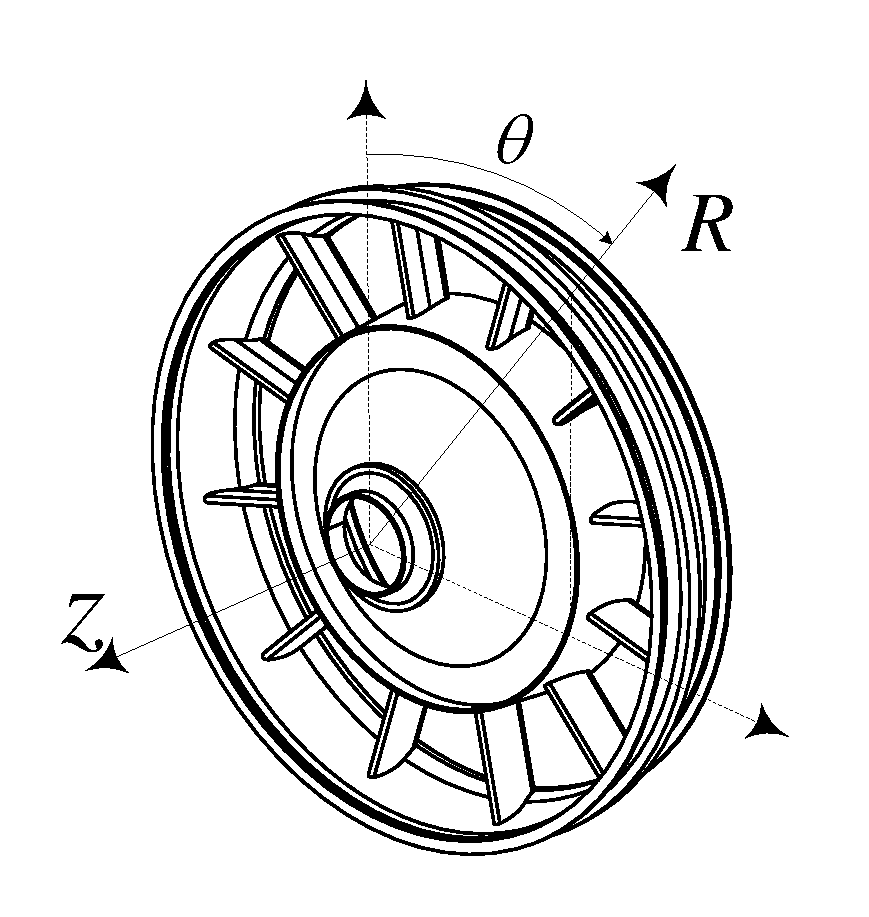
\includegraphics[width=0.3\textwidth]{1a_TRS_isometric}} \hspace{0.1\textwidth}%
	\subfloat[Deposition variables \label{fig:stiffdims}]{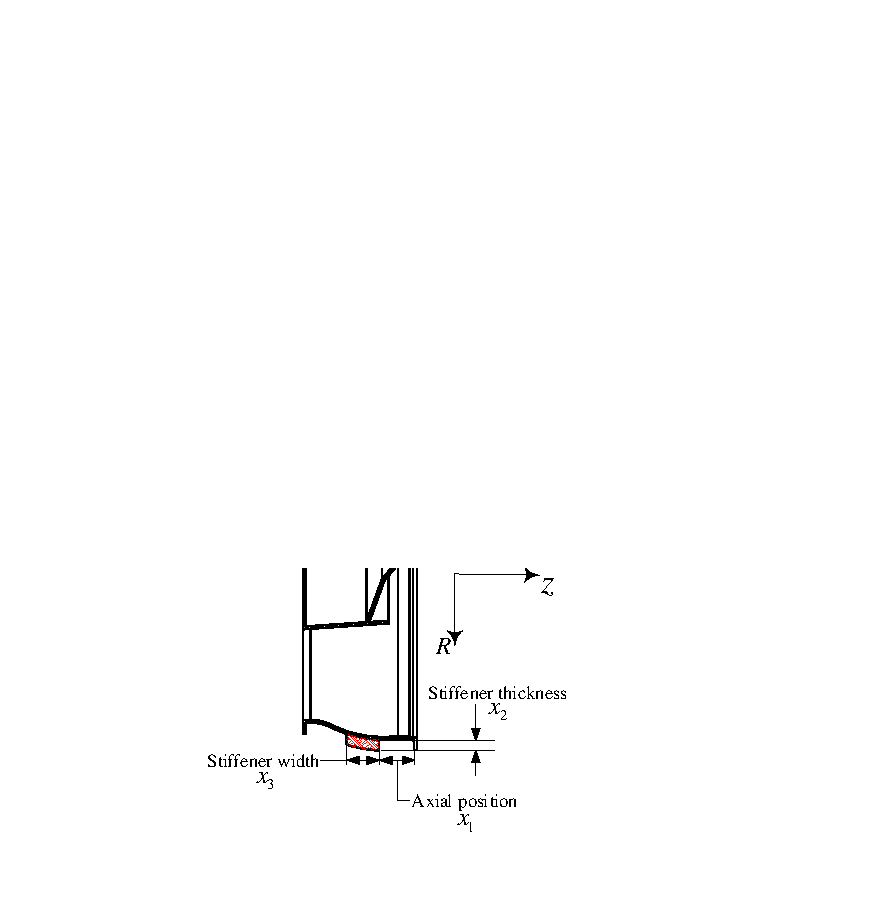
\includegraphics[width=0.3\textwidth]{1b_TRS_overview}}	
	\caption{TRS stiffener example}
	\label{fig:TRSoverview}
\end{figure}

Comprehensive thermomechanical models feature a coupled transient heat transfer and fluid flow model to accurately calculate the transient temperature field. The temperature field is used for residual stress and distortion modeling \cite{Mukherjee2017}. Complex physical processes govern the temperature field making its computation intensive. Computations of the temperature field involve various simplifications and assumptions to make the calculations tractable. \citeauthor{Manvatkar2011} consider a \ac{FEA} conduction model for calculating the transient temperature field due to a moving Gaussian heat source on the substrate \cite{Manvatkar2011}. The problem of a moving heat source on an infinite plate was formulated and solved analytically by \citeauthor{rosenthal1946theory} \cite{rosenthal1946theory}. The Rosenthal model is used for cases where there is limited heat conduction in the through thickness dimension typical of thin plates \cite{Goldak1984}. The \ac{TRS} outer casing where the stiffener is to be deposited has a through thickness dimension considerably smaller than its width and circumference allowing us to approximate the heat source by a Gaussian heat source as in the Rosenthal model.

The melt pool dimensions are estimated from the transient thermal model to determine the deposit width and depth. Figure~\ref{fig:gaussian} shows the details of the thermomechanical simulations for determining deposit size. A Gaussian heat source with a heat flux distribution given by Equation~(\ref{eg:gaussian}) scans the surface at a constant speed ${\color{black}{V}}$ \cite{rosenthal1946theory}

\begin{equation}
	Q(r,\theta,t) = \dfrac{\color{black}{P}}{\pi{\color{black}{r_l}}^2 D_p}e^{-2\left(\frac{r-{\color{black}{V}}t}{\color{black}{r_l}}\right)^2}, \label{eg:gaussian}
\end{equation}

where ${\color{black}{r_l}}$ is the laser beam radius, ${\color{black}{P}}$ is the laser power and $D_p$ is the depth of penetration of the laser source. The coordinates $r$ and $\theta$ are defined on the surface of the deposit as shown in Figure~\ref{fig:gaussianheat}. 

\begin{figure}[h!]
	\centering
	\subfloat[Gaussian heat source\label{fig:gaussianheat}]{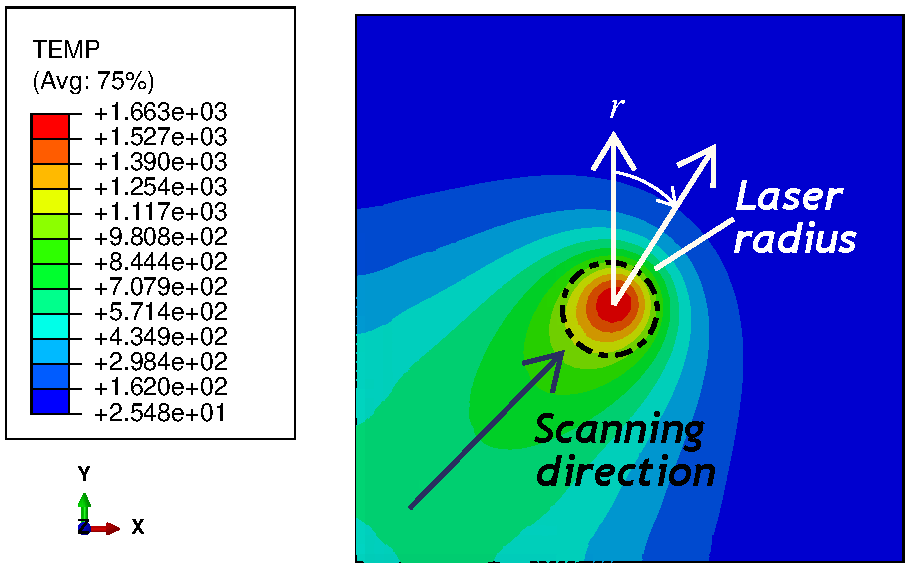
\includegraphics[width=0.45\textwidth]{2a_guassian_heat}} \hspace{0.1\textwidth}%
	\subfloat[Melt pool  \label{fig:pooldims}]{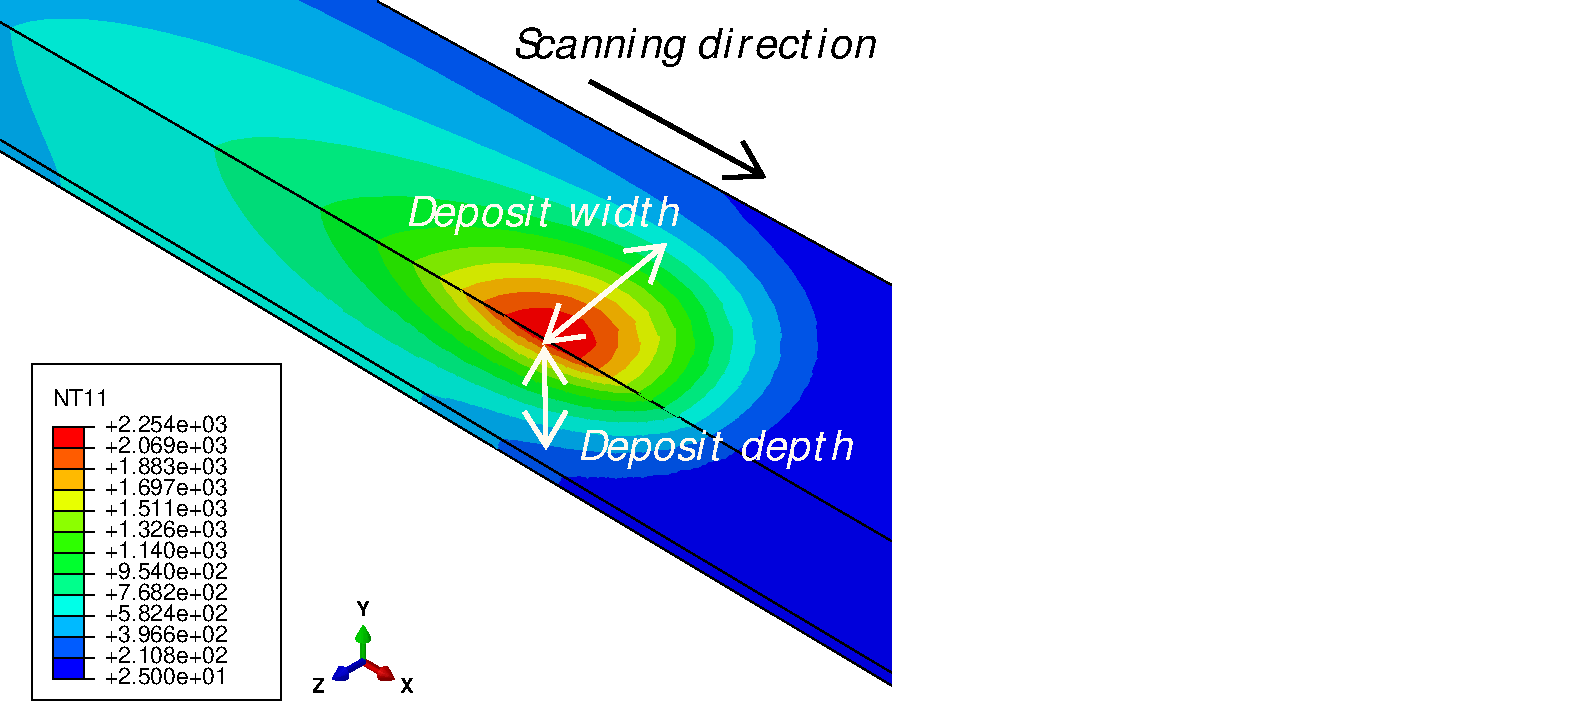
\includegraphics[width=0.29\textwidth]{2b_pool_dims}}	
	\caption{Heat conduction for a moving Gaussian heat source}
	\label{fig:gaussian}
\end{figure}

The resulting deposit width $D_w$ and depth $D_d$ are used to partition the stiffener geometry into $n_l$ by $n_d$ deposits in the axial and radial directions, respectively, where $n_l = \round{x_3/D_w}$ and $n_d = \round{x_2/D_d}$. 

For the deposition on the \ac{TRS} outercasing, a further simplification of the transient conduction model can be made by applying the heat flux uniformly on the surface of the deposit \cite{Nickel2001}. We use a static model with a uniformly distributed heat flux to compute residual stresses. This idealization (relative to using a transient heat transfer model) reduces the number of variables and parameters involved and alleviates computational cost by exploiting TRS symmetry without sacrificing accuracy excessively.

Each deposit is heated uniformly by an equivalent heat flux that supplies the same energy as a moving Gaussian heat source scanning the entire deposit surface. The power at $t=0$ is given by the surface integral of the heat flux over an infinite plane

\begin{equation}
	\label{eq:power}
	P(t=0) = \dfrac{\color{black}{P}}{\pi{\color{black}{r_l}}^2 D_p} \Int_{0}^{2\pi} \Int_{0}^{\infty} e^{-2\left(\frac{r}{\color{black}{r_l}}\right)^2} \,rdr\,d\theta = \dfrac{\color{black}{P}}{\pi{\color{black}{r_l}}^2 D_p}\dfrac{\pi{\color{black}{r_l}}^2}{2} = \dfrac{\color{black}{P}}{2D_p}.
\end{equation}


The power per unit depth $P(t=0)$ is multiplied by the scanning time $t_{scan}$ to obtain the heat energy input to the deposit. The scanning time is calculated for each stiffener by dividing total distance traveled by the heat source (stiffener length) by the scanning speed $t_{scan} = L/{\color{black}V}$. $A_{\textrm{stiff}}$ is the surface area of the stiffener where heat is applied. These values are obtained from the geometry of the stiffener using \ac{CAD} tools.

The energy is divided by an equivalent step time $t_{\textrm{step}}$ used for static thermal analysis in lieu of a transient thermal analysis to obtain the equivalent uniformly distributed power per unit depth $P_{\textrm{eqv}}$. $P_{\textrm{eqv}}$ is divided by the area of the deposit $A_{\textrm{stiff}}$ to yield the equivalent heat flux per unit depth $Q_{\textrm{eqv}}$:

\begin{equation}
	\label{eq:powereqv}
	Q_{\textrm{eqv}} = \dfrac{P_\textrm{laser}}{2D_{p}}\dfrac{t_{\textrm{scan}}}{t_{\textrm{step}}}\dfrac{1}{A_{\textrm{stiff}}}.
\end{equation}

A special case of stiffener is the circumferential stiffener shown in Figure~\ref{fig:TRSoverview}. For this type of stiffener, Equation~(\ref{eq:powereqv}) can be simplified by setting $L = 2\pi R_{\textrm{outer}}$, where $R_{\textrm{outer}} = 0.5$ m is the radius of the outer casing of the \ac{TRS}. This results in $t_{scan} = 2\pi R_{\textrm{outer}}/{\color{black}V}$. The deposit surface area becomes $A_{\textrm{deposit}} = 2\pi {R_{\textrm{outer}}}D_w$ to yield the equivalent heat flux per unit depth:

\begin{equation}
	\label{eq:powereqvcirc}
	Q_{\textrm{eqv}} = P(t=0)\dfrac{2\pi R_{\textrm{outer}}}{{\color{black}V}}\dfrac{1}{t_{\textrm{step}}}\dfrac{1}{2\pi {R_{\textrm{outer}}}D_w} = P(t=0)\dfrac{1}{{{\color{black}V}}t_{\textrm{step}}D_w} = \dfrac{{\color{black}P}}{{2{\color{black}V}}t_{\textrm{step}}D_wD_p}.
\end{equation}

We assume here that the radius of the deposit is equal to the radius of the outer casing $R_{\textrm{outer}}$ since the thickness of the deposit is small relative to the outer casing.

An example of the application of $Q_{\textrm{eqv}}$ to the surface of a circumferential deposit layer is shown in Figure~\ref{fig:depload}.

\begin{figure}[h!]
    \centering
    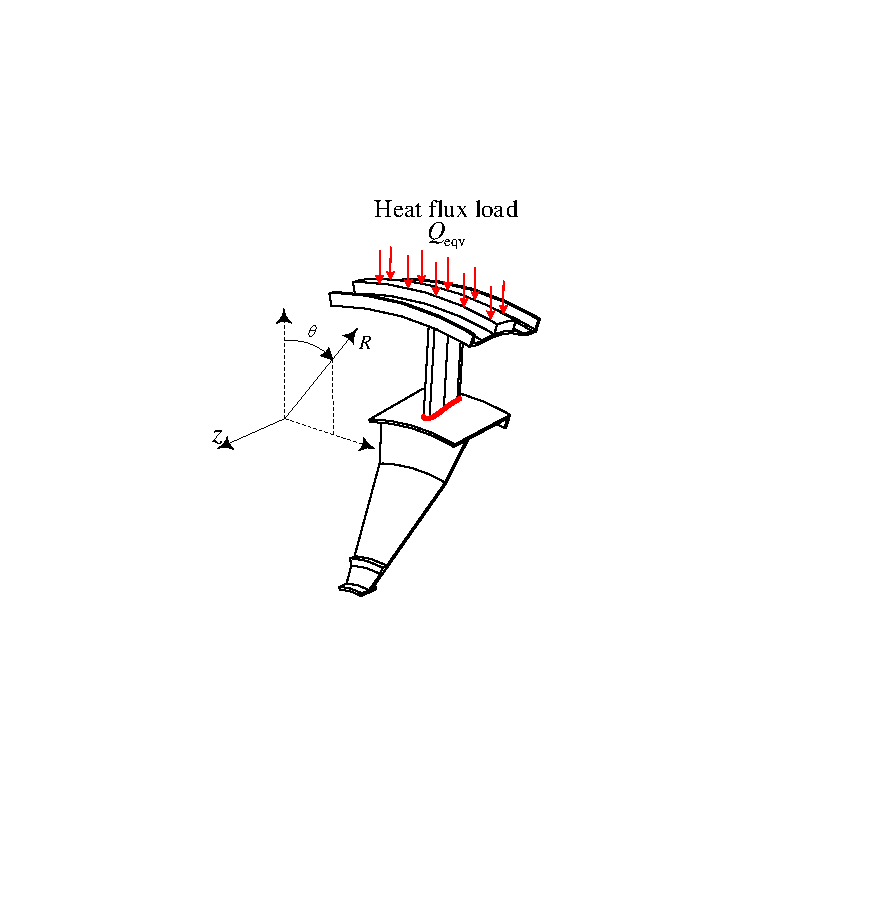
\includegraphics[width=0.4\textwidth]{3a_heat_load.pdf}
    \caption{ \label{fig:depload} Deposition load }
\end{figure}

After obtaining the thermal gradients due to the application of the heat flux load, the corresponding thermal stresses are computed. The stresses that persist after removal of the heat flux load are the residual stresses. These residual stresses are inherent in the structure and affect the structural performance of the \ac{TRS} during subsequent operational loads. 

The maximum and minimum residual principal stresses along the circumference of the \ac{TRS} outer casing are shown in Figure~\ref{fig:Sprinciple} for both static and transient models. Table~\ref{table:validation} summarizes the utilized parameter values for this comparative study.

\begin{table}[h!]
\centering
\renewcommand{\arraystretch}{1.0}% Wider
\small\addtolength{\tabcolsep}{-5pt}
\caption{Comparison of transient and static models: parameter values}
\label{table:validation}
\begin{tabular}{lcccc}
\hline\hline
\bf Parameter & \bf Notation & \bf Units & \bf Value \\\\ \hline
Stiffener axial position & $x_1$ & mm & 80.0  \\
Stiffener thickness  & $x_2$ & mm & 4.0  \\
Stiffener width & $x_3$ & mm & 23.5  \\
Laser Power & ${P}$ & W & 3,889.13 \\ 
Laser beam radius & ${r_l}$ & mm & 13.63 \\ 
Scanning speed& ${V}$ & mm/s & 5.0 \\ 
Number of layers & $n_l$ & - & 2\\
Number of deposits (transverse) & $n_d$ & - & 1\\
Deposit depth  & $D_d$ & mm & 2.01\\
Deposit width  & $D_w$ & mm & 25.0 \\
Deposit surface area  & $A_\textrm{deposit}$ & mm$^2$ & \num{8.304e4} \\
Equivalent heat flux per unit depth & $Q_\textrm{eqv}$ & W/mm$^3$ & 0.8138 \\
\hline\hline
\end{tabular}
\end{table}

In all our analyses throughout the thesis, the scanning speed is considered constant at a nominal value of ${\color{black} V} = 5$ mm/s.

\begin{figure}[h!]
	\centering
	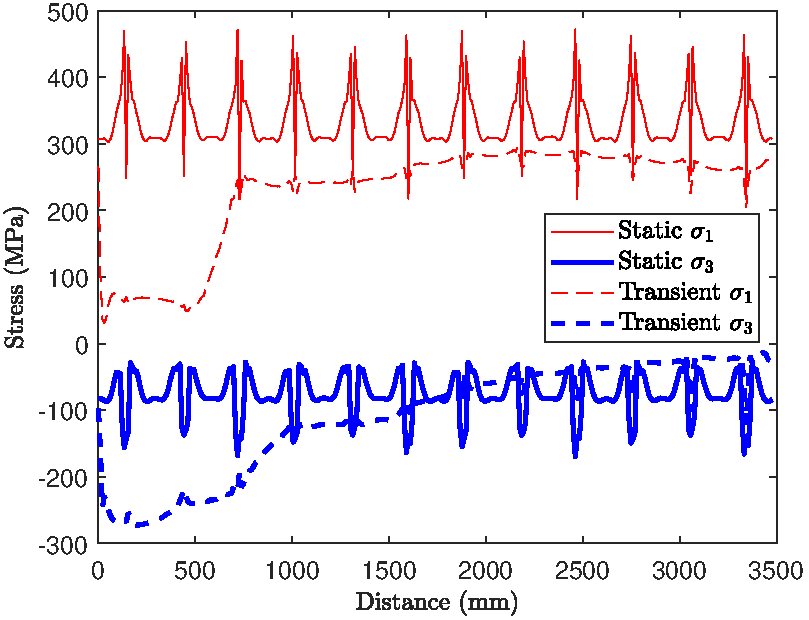
\includegraphics[width=0.6\textwidth]{6_residual_stresses.pdf}
	\caption{ \label{fig:Sprinciple} Spatial distribution of principle residual stresses along the circumference of the \ac{TRS} obtained using transient and static models}
\end{figure}

The principal stresses provide an indication of the compressive or tensile nature of the stress state and will be used in subsequent failure analysis to determine the safety factor. There is a general agreement in the value of the predicted stresses with lower values recorded for the transient model due to the time taken by the substrate to reach steady state temperatures as the heat source scans its surface. Furthermore, the static model overpredicts the maximum principal stress making it a more conservative choice for thermomechanical modelling.

In the following section we describe the different load cases that the \ac{TRS} may experience in operation

%============================= LOAD CASES ==============================%
\section{Load cases applied to turbine rear structure}
\label{sec:loadcases}

The \ac{TRS} experiences a number of thermal and mechanical loads due to the exhaust gases it directs while providing structural support to the engine. Two significant load cases are used for the analyses in this thesis to address the uncertainty involved in their parameters and their significance regarding the functionality of the \ac{TRS}.

We describe the first load case in the following section.

%---------------------------------------------------------------------%
% Pressure load case
\subsection{Pressure load case} \label{subsec:iploadcase}

\begin{figure}[h!]
    \centering
    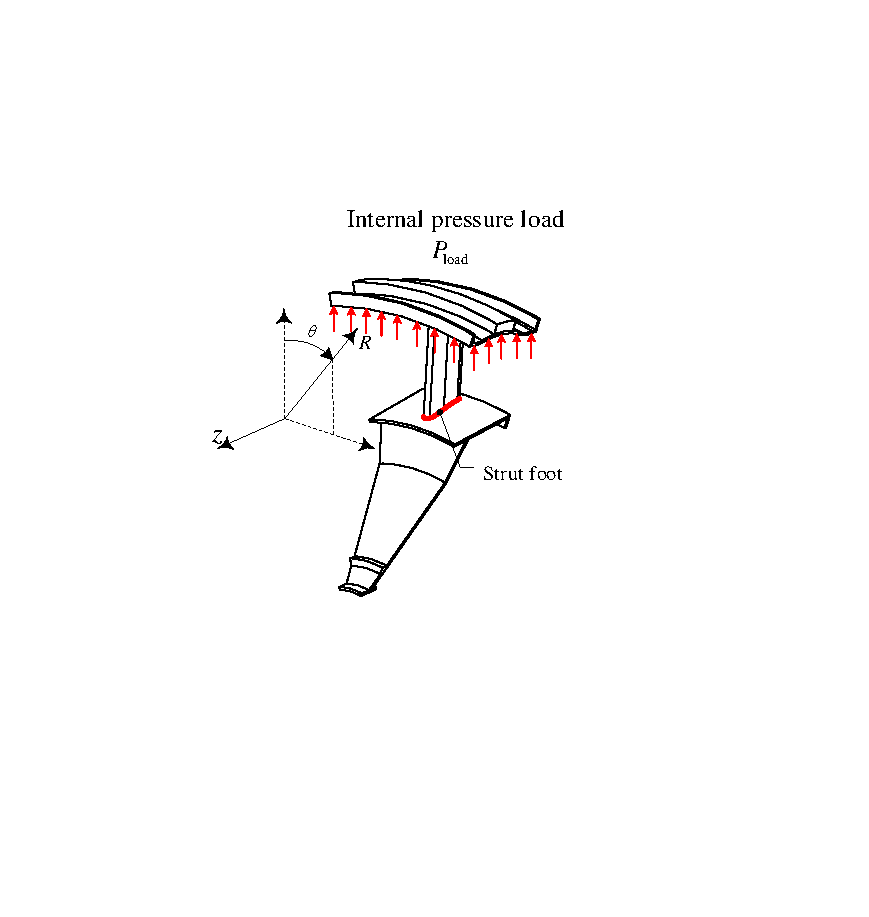
\includegraphics[width=0.4\textwidth]{3b_pressure_load.pdf}
    \caption{ \label{fig:ipload} \ac{TRS} pressure load case }
\end{figure}

The first load case is due to the internal pressure $P_{\textrm{load}}$ applied on the outer casing of the \ac{TRS} by the hot exhaust gases. A pressurization/depressurization cycle is shown in Figure~\ref{fig:ipload}. The load case is cycled and is used to compute the expected fatigue life of the \ac{TRS} using low-cycle fatigue calculations. The stress state at the foot of a strut (shown in Figure~\ref{fig:ipload}) is monitored before and after the load case to obtain the initial and final Von mises stresses $\sigma_{v1}$ and $\sigma_{v2}$, respectively. Note that $\sigma_{v1} \neq 0$ due to the residual stress state in the structure from prior thermomechanical loads. 

We now describe the thermal loadcase due to the temperature of the exhaust gases.

%---------------------------------------------------------------------%
% Thermal load case
\subsection{Thermal load case} \label{subsec:thermalloadcase}

The \ac{TRS} shown in Figure~\ref{fig:TRSiso} is subject to thermal loads due to the temperature gradients it experiences during operation. The temperature profile of a \ac{TRS} during operation is shown in Figure~\ref{fig:thermalloads}. These temperature loads are specified by the engine architect to the \ac{TRS} \ac{OEM} in the form of uncertain parameters.

\begin{figure}[h!]
	\centering
	\subfloat[Safety factor calculation domain \label{fig:TRSiso}]{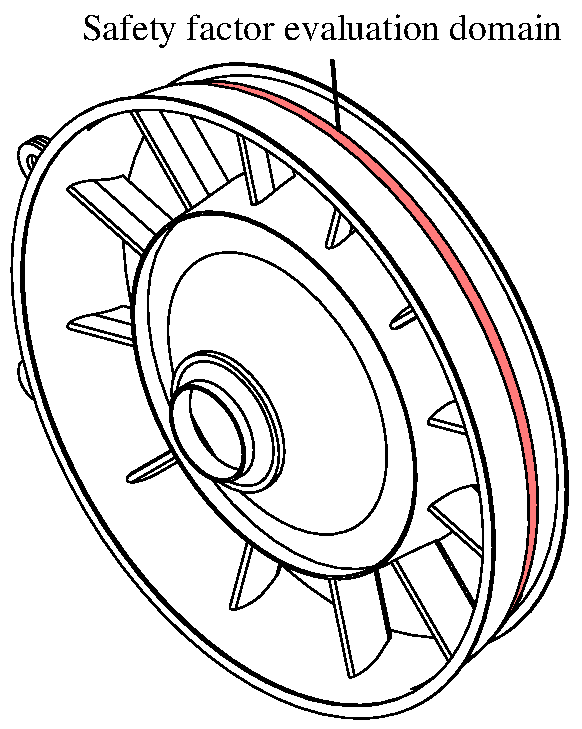
\includegraphics[width=0.275\textwidth]{5a_TRS_isometric}} \hspace{0.1\textwidth}%
	\subfloat[Thermal loads \label{fig:thermalloads}]{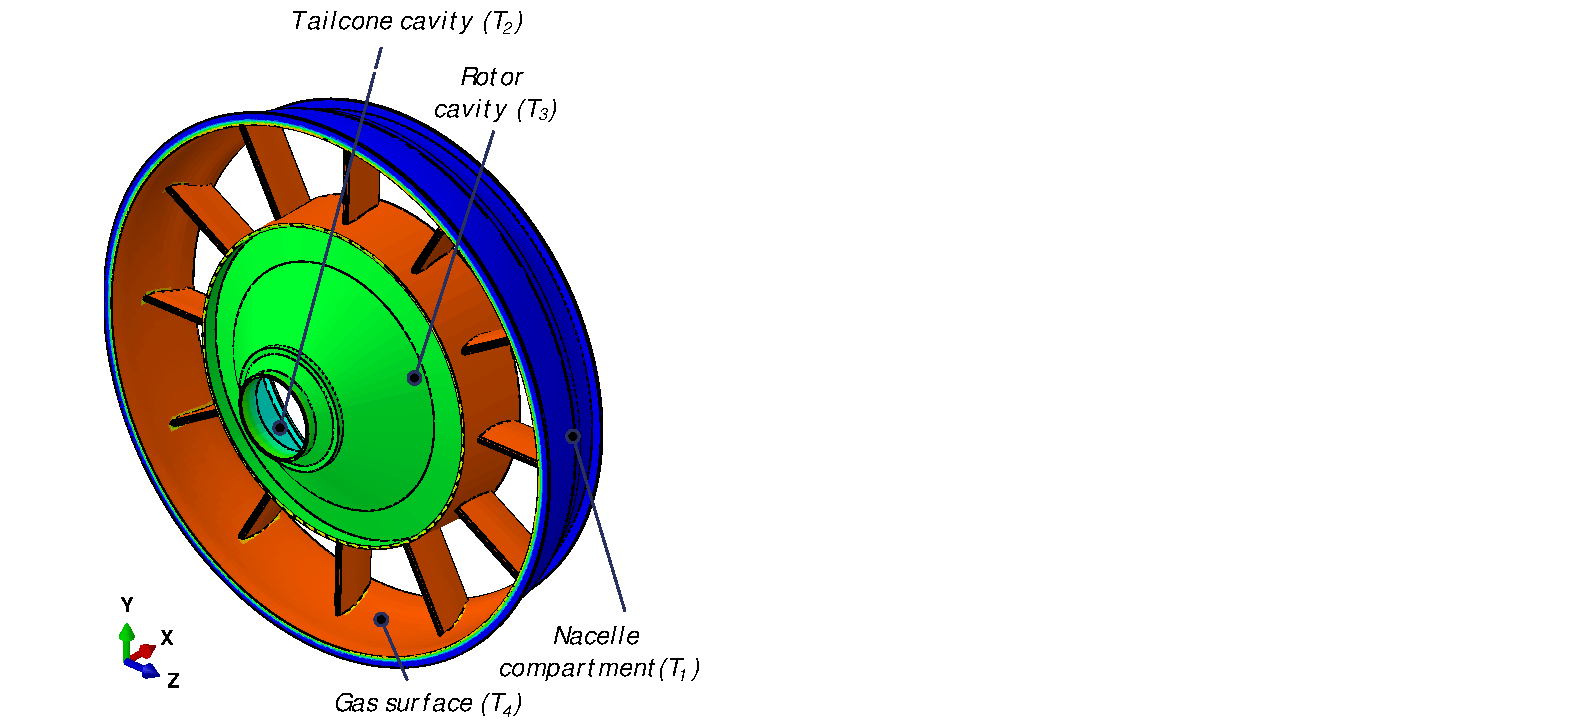
\includegraphics[width=0.3125\textwidth]{5b_thermal_loadcase}}
	\caption{\ac{TRS} thermal load case}
	\label{fig:thermalloadcases}
\end{figure}

The thermal load case is cycled and is used to compute the expected fatigue life of the \ac{TRS} using low-cycle fatigue calculations. We restrict the low-cycle fatigue analysis to the midsection of the outercasing shown in Figure~\ref{fig:TRSiso} in order to simplify computation and postprocessing. The stress state at the midsection of the outercasing is recorded before and after the load case to obtain the initial and final Von Mises stresses $\sigma_{v1}$ and $\sigma_{v2}$, respectively. 

The structural analyses presented for the thermomechanical, pressure and thermal load cases is performed using a \ac{FE} simulation model which is computationally expensive. As a result, we will construct surrogates for these models in Chapters \ref{ch:scalableSBD}, \ref{ch:TSEcont} and \ref{ch:stohasticopt} to alleviate the computational effort involved in exploring the design and parameter spaces for these problems.

We explain how the safety factor $n_{\textrm{safety}}(\mathbf{p})$ is computed for these load cases in the following section.

%---------------------------------------------------------------------%
% Fatigue calculation
\subsection{Low-cycle fatigue analysis} \label{subsec:fatigueanalysis}

We use the initial and final Von Mises stresses $\sigma_{v1}$ and $\sigma_{v2}$ obtained before and after the application of either load case described earlier to compute the safety factor against low-cycle fatigue.

The midrange stress ($\sigma_m = -\textrm{sign}(\sigma_P)\left( \sigma_{v1} + \sigma_{v2}\right) / 2$) and the amplitude stress ($\sigma_a = \left| \sigma_{v1} - \sigma_{v2}\right| / 2$) are calculated, where $\textrm{sign}(\sigma_P)$ is the sign of the pressure given by the sum of the principle stresses ($\sigma_P = -(1/3) (\sigma_1 + \sigma_2 + \sigma_3)$) and provides of measure of the compressive or tensile state of the stress. A negative $\sigma_P$ implies tension while a positive value implies compression. The failure locus is determined by the modified Goodman criterion for high cycle fatigue as shown in Figure~\ref{fig:GMcrit}. The endurance limit ($S_e$), yield stress ($\sigma_y$) and ultimate strength ($S_{ut}$) are defined as parameters and are obtained from mechanical design handbooks \cite{Budynas2015}. The number of lifecycles to failure is estimated from W{\"o}hler relations ($N_f = \left(\sigma_{\textrm{rev}}/a\right)^b$), where $a$ and $b$ are empirical constants. The safety factor is calculated as $n_{\textrm{safety}} = 1/\left({\frac{\sigma_a}{S_e}+\frac{\sigma_m}{S_{ut}}}\right)$ for each load case.

\begin{figure}[h!]
    \centering
    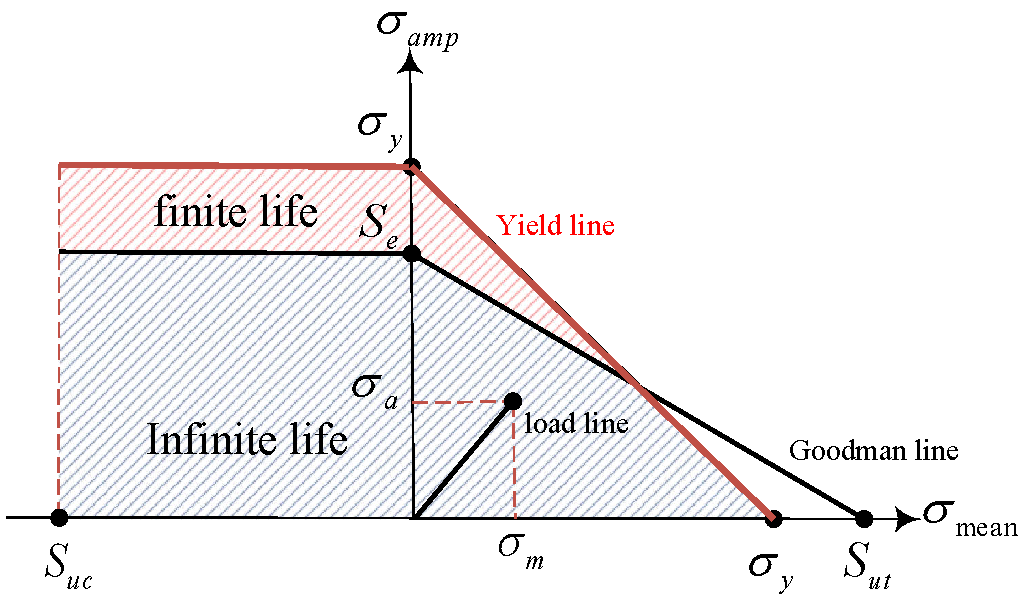
\includegraphics[width=0.7\textwidth]{4_Fatigue_loading.pdf}
    \caption{ \label{fig:GMcrit} Modified Goodman criterion }
\end{figure}

The safety factor $n_{\textrm{safety}}$ is used as a structural performance metric throughout this thesis. We know summarize all the relevant inputs and outputs to the introduced thermomechanical models and loadcases.

%============================== SUMMARY ================================%
\section{Summary}
\label{sec:thermosummary}

This chapter presented the industrial case study that will be use throughout the thesis to demonstrate the developed frameworks. The chapter defined the thermomechanical model and two loadcases that the \ac{TRS} experiences in operation. The loadcase parameters and outputs are summarized in Tables \ref{table:parametervar} and \ref{table:modeloutputs}. Some parameters in Table \ref{table:parametervar} are uncertain and are denoted by ranges. They will be elaborated on during the analysis in the following chapters.

\begin{table}[h!]
	\centering
	\renewcommand{\arraystretch}{1.0}% Wider
	\normalsize\addtolength{\tabcolsep}{-5pt}
	\caption{Model design parameters}
	\label{table:parametervar}
	\begin{tabular}{lcc>{\centering\arraybackslash}p{3cm}>{\centering\arraybackslash}p{2cm}}
	\hline\hline
	\bf Parameter & \bf Notation & \bf Units & \bf Value \\ \hline
	Stiffener axial position & $x_1$ & mm & $91 \pm 54$ \\
	Stiffener thickness  & $x_2$ & mm & $6 \pm 4$ \\
	Stiffener width & $x_3$ & mm & $25 \pm 15$  \\
	Laser Power & ${P}$ & W & $3750 \pm 250$\\ \hline
	Internal pressure load  & ${P}_{\textrm{load}}$ & MPa & $2 \pm 0.5$ \\ 
	Deposit melting point & $T_m$ & $^o$C & $1,500 \pm 100$ \\
	Substrate base width & $W_{\textrm{total}}$ & mm & $137.5 \pm 17.5$ \\
	Nacelle temperature & $T_1$ & $^{o}$C & $300 \pm 100$ \\ 
	Tailcone temperature & $T_2$ & $^{o}$C & $400 \pm 100$ \\ 
	Rotor temperature & $T_3$ & $^{o}$C & $450 \pm 100$ \\ 
	Gas surface temperature & $T_4$ & $^{o}$C & $600 \pm 100$ \\
	\hline
	%================================================================
	Laser beam radius & ${r_l}$ & mm & 14.2 \\ 
	Scanning speed& ${V}$ & mm/s & 5.0 \\ 
	Laser penetration depth & $D_p$ & mm & 5.0 \\
	%================================================================
	\hline\hline
	\end{tabular}
\end{table}

\begin{table}[h!]
	\centering
	\renewcommand{\arraystretch}{1.0}% Wider
	\normalsize\addtolength{\tabcolsep}{-5pt}
	\caption{Relevant model outputs}
	\label{table:modeloutputs}
	\begin{tabular}{lcc}
	\hline\hline
	\bf Output    & \bf Notation & \bf Units \\ \hline
	Number of layers & $n_l$ & - \\
	Number of deposits (transverse) & $n_d$ & - \\
	Deposit depth  & $D_d$ & mm \\
	Deposit length  & $D_l$ & mm \\
	Deposit width  & $D_w$ & mm \\
	Deposit surface area  & $A_\textrm{stiff}$ & mm$^2$ \\
	Deposit length  & $L$ & mm \\
	Scanning time  & $t_\textrm{scan}$ & s \\
	Equivalent heat flux  & $Q_\textrm{eqv}$ & W/mm$^2$ \\
	Safety factor against low-cycle fatigure & $n_{\textrm{safety}}$ & - \\
	Number of lifecycles to failure (${P}_{\textrm{load}}$)& $N_f$ & - \\
	Deposition temperature & $T_\textrm{deposit}$ & $^o$C \\
	\hline\hline
	\end{tabular}
\end{table}

We describe the methodology for obtaining scalable design solutions for product remanfuacturing in the following chapter. The internal pressure loadcase described in Section~\ref{subsec:iploadcase} will be used to demonstrate this framework. The thermal loadcase described in Section \ref{subsec:thermalloadcase} will be used for demonstrating the design margin allocation tool developed in Chapter \ref{ch:TSEcont}.

% Chapter 04: Scalable SBD
%%%%%%%%%%%%%%%%%%%%%%%%%%%%%%%%%%%%%%%%%%%%%%%%%%%%%%%
%%                SBD scalable design                %%
%%%%%%%%%%%%%%%%%%%%%%%%%%%%%%%%%%%%%%%%%%%%%%%%%%%%%%%
\chapter{Scalable set based design optimization}
\chaptermark{Scalable set based design optimization}
\label{ch:scalableSBD}
%%%%%%%%%%%%%%%%%%%%%%%%%%%%%%%%%%%%%%%%%%%%%%%%%%%%%%%

This chapter describes a novel design tool for identifying a set of scalable designs for product remanufacturing using parametric design optimization. Scalability is an enabler for product remanufacturing since it provides components with the flexibility to have their specifications upgraded to meet higher requirement levels.

The methodology in this chapter is demonstrated using an industrial application example for the remanufacturing design of a \ac{TRS}. The thermomechanical model described in Section~\ref{sec:thermomech} along with the load case in Section~\ref{subsec:iploadcase} is used to define the design variables and uncertain parameters involved in the remanufacturing design problem. Remanufacturing is performed by \ac{AM} using laser \ac{DED}. However, our methodology can be extended to remanufacturing problems where subtractive manufacturing is used.

We begin by defining the methodology for obtaining the set-based solutions for arbitrary design and parameter spaces in Section~\ref{sec:SBDmethods}. We then demonstrate the methodology for the remanufacturing of the \ac{TRS} in Section~\ref{sec:SBDusecase}. We provide some insights and conclusions about the uses and limitations of the developed framework in Section~\ref{sec:scalableSBDsummary}.

%============================ METHODOLOGY ============================%
\section{Methodology} \label{sec:SBDmethods}

Engineering design optimization problems involve decision variables $\mathbf{x}  \in \mathbb{R}^n$ and design parameters ${\mathbf{p}}  \in \mathbb{R}^m$. Objective (${f}(\mathbf{x};\mathbf{p})$) and constraint ($\mathbf{g}(\mathbf{x};\mathbf{p})$) functions are used to reflect design requirements. Given bounded design optimization variables and parameters $\mathbf{L} \leq \mathbf{x} \leq \mathbf{U}$ and $\mathbf{L}_p \leq \mathbf{p} \leq \mathbf{U}_p$, respectively, we define the design space $\mathit{D}$ and the parameter space $\mathit{P}$. We also consider constraint sets $\mathit{C}_u$ for $u = 1,2,\ldots,q$ where $q$ is the number of constraints. In a product design context, constraints are part of the design requirements and are driven by the parameters $\mathbf{p}$. Finally, the feasible set $\mathit{F}$ is defined as the intersection of all constraint sets and contains designs that meet all design requirements. The set $\mathit{F}$ is the \ac{FDS} and represents the outcome of \ac{SBD} before elimination of potential designs. 

Design parameters may affect the optimal solution of the optimization problem due to their influence on design requirements. As a result, designs that are optimal throughout the parameter space $\mathit{P}$ and satisfy the design requirements comprise the set of parametric optimal designs which is a reduction of the \ac{FDS}. Since practical \ac{SBD} methodolog\-ies require solutions sets that can be easily communicated across design teams, response surfaces are used as a surrogate model to evaluate feasibility and performance and to classify membership of each design to the feasible set and the set of parametric optimal designs. 

% --------------------------- Surrogate modeling ------------------------------ %
\subsection{Surrogate modeling} \label{subsec:RSM}

The objective and constraint functions used to represent design requirements are evaluated using computer-aided engineering (CAE) tools that model the repair/remanufacturing process.  
These computational models are computationally expensive. Any SBD methodology requires a large number of function evaluations to investigate not only the design but also the parameter space. Therefore, we resort to building less expensive response surfaces to be used as surrogate models.

We conduct designs of experiments to sample the aggregate design and parameter spaces and then exercise the computational models at these sample points to generate adequate training data. An ensemble of surrogate models is then constructed and denoted by $\hat{f}(\mathbf{x};{\mathbf{p}})$ and $\hat{\mathbf{g}}(\mathbf{x};{\mathbf{p}})$. An open source surrogate model library is used to build the surrogates \cite{Talgorn2018,Lophaven2002}.

An order-based metric is used to assess the predictive capability of the surrogates \cite{Audet2018}. This metric ensures the consistency between the computationally expensive and surrogate model predictions. The order-based metric is also used for constructing response surfaces of the parametric optimal solutions with respect to varying design parameters in subsequent sections and is discussed using a numerical example in Section~\ref{subsec:numex}.
% is a measure of how well the ordering of function values throughout the analysis model agrees with that of the \ac{SM}. If this condition is observed in the response surface \ac{SM}, the solution to the minimization problem of the analysis model $f(\mathbf{x})$ and the surrogate model $\hat{f}(\mathbf{x})$ should be consistent. The conditions can be stated as follows and are adopted from \cite{Audet2018}:
%
%\begin{gather}
%	f(\mathbf{x}) \leq f(\mathbf{x}') \Leftrightarrow \hat{f}(\mathbf{x}) \leq \hat{f}(\mathbf{x}'),~\textrm{for all}~\mathbf{x}, \mathbf{x'} \in \mathit{D} \label{eq:oeobjective}\\
%	g_u(\mathbf{x}) \leq 0 \Leftrightarrow \hat{g_u}(\mathbf{x}) \leq 0,~\textrm{for all}~\mathbf{x}, \in \mathit{D}\label{eq:oeconstraints}
%\end{gather}
%
%The frequency of violation of these rules is an indicator of the surrogate model's deficiency in capturing the global minima of its corresponding analysis model. It should also be noted that any insensitive parameters or variables should be eliminated from the analysis to alleviate the computational effort of obtaining an efficient surrogate model for optimization in terms of the \ac{OE} criterion. This elimination is demonstrated at the end of Section~\ref{subsec:thermomech}.

% --------------------------- Design space reduction based on optimization ------------------------------ %
\subsection{Parametric optimal designs} \label{subsec:SBDparametric}

We use numerical optimization to provide a set of design solutions that can address  a range of requirements. Specifically, we solve the optimization problem for different parameter values. This can be seen as a form of \ac{POA} that provides the sensitivity of optimal design variable values with respect to varying parameter values \cite{Sobieszczanski-Sobieski1982}.

The surrogate optimization problem is formulated as
\begin{equation}
	\begin{aligned}
		& \underset{\mathbf{x}}{\text{minimize}}
		& & \hat{f}(\mathbf{x};{\mathbf{p}})\\
		& \text{subject to}
		& & \hat{\mathbf{g}}(\mathbf{x};{\mathbf{p}}) \le \mathbf{0}
	\end{aligned}
	\label{eq:SBDoptproblem}
\end{equation}
and solved to obtain the solution $\mathbf{x}^*({\mathbf{p}})$. Given intervals for the parameters $\mathbf{p}$, sampling techniques can be used to obtain a set of $m$ combinations. Here, we use \ac{LH} sampling which produces a uniform random distribution over the parameter space \cite{McKay1979}
\begin{equation}
	 {\mathbf{P}} = \begin{bmatrix}
	 	\mathbf{p}_{1}^{\text T} \\ 
	 	\mathbf{p}_{2}^{\text T} \\ 
	 	\vdots \\ 
	 	\mathbf{p}_{w}^{\text T}
	\end{bmatrix} = \begin{bmatrix}
	 	p_{11} & p_{12} & \cdots & p_{1m}\\ 
	 	p_{21} & p_{22} & \cdots & p_{2m}\\ 
	 	\vdots & \vdots & \ddots & \vdots\\ 
	 	p_{w1} & p_{w2} & \cdots & p_{wm}
	\end{bmatrix}.
\end{equation}

\ac{LH} sampling is used since the number of samples needed to fit an adequate response surface scales better with dimensionality relative to uniform sampling techniques such as full factorial sampling. Once we have obtained a solution $\mathbf{x}^*({\mathbf{p}})$ for each of the $w$ parameter vectors, a response surface $\hat{\mathbf{x}^*}(\mathbf{p})$ is built using the set of parametric optimal designs $\mathbf{X}^*=  \{ \mathbf{x}^*(\mathbf{p}_1),\mathbf{x}^*(\mathbf{p}_2),\ldots,\mathbf{x}^*(\mathbf{p}_w) \}$. A rule of thumb indicates that the initial sample size should be about an order of magnitude larger than the dimensionality of the problem, i.e., $w \approx 10m$) \cite{Loeppky2008}. To potentially save computational cost, we also monitor the convergence rate of the order-based error as more samples are added and accept the response surface as adequate once it has reached an appropriate threshold. An example of this procedure is provided in Section~\ref{subsec:numex}. The response surface $\hat{\mathbf{x}^*}(\mathbf{p)}$ is used to predict parametric optimal designs throughout the parameter space.

Sensitivity gradients of the design variables with respect to the parameters allow designers to understand the effect of requirement changes to optimal designs.
The Jacobian of $\hat{\mathbf{x}^*}(\mathbf{p})$ is
\begin{equation}
	\mathbf{J}(\mathbf{p}) = \nabla\hat{\mathbf{x}^*}(\mathbf{p)} = \begin{bmatrix}
	 	\nabla\hat{x_1^*}^{\text T}(\mathbf{p}) \\ 
	 	\nabla\hat{x_2^*}^{\text T}(\mathbf{p}) \\ 
	 	\vdots \\ 
	 	\nabla\hat{x_n^*}^{\text T}(\mathbf{p})
	\end{bmatrix} = \begin{bmatrix}
	 	\frac{\partial \hat{x_1^*}}{\partial p_1} & \frac{\partial \hat{x_1^*}}{\partial p_2} & \cdots & \frac{\partial \hat{x_1^*}}{\partial p_m}\\ 
	 	\frac{\partial \hat{x_2^*}}{\partial p_1} & \frac{\partial \hat{x_2^*}}{\partial p_2} & \cdots & \frac{\partial \hat{x_2^*}}{\partial p_m}\\ 
	 	\vdots & \vdots & \ddots & \vdots\\ 
	 	\frac{\partial \hat{x_n^*}}{\partial p_1} & \frac{\partial \hat{x_n^*}}{\partial p_2} & \cdots & \frac{\partial \hat{x_n^*}}{\partial p_m}\\ 
	\end{bmatrix}.
	 \label{eq:jacobian}
\end{equation}
It can be estimated using the derivatives of the basis functions used to construct the response surface. Differentiation of the response surface is possible because it is based on a linear combination of basis functions. We use a \acf{KS} model to build  $\hat{\mathbf{x}^*}(\mathbf{p})$ and estimate the Jacobian $\mathbf{J}(\mathbf{p})$ using the linear combination of the gradient of the kernel functions. \ac{KS} was used to construct the response surface due to their immediate computation since it does not require matrix inversions. Furthermore, \ac{KS} models typically respect the order of the output which reflects its ability to predict the correct order of values of any two evaluation points. This is very important for this application since it relies on differentiating the KS model \cite{Audet2018}.

For the remainder of this subsection, let us use the typical notation between an independent variable $x$ and a dependent variable $y$ recalling however, that in our context $\hat{\mathbf{x}^*}(\mathbf{p})$ is corresponding to $y$ (dependent variable) while $\mathbf{p}$ is corresponding to $x$ (independent variable).

\ac{KS} models consist of a weighted sum of training points where the weight for each training point decreases as the distance from the prediction point increases.
\begin{multline}
 \label{eq:ksexpansion}
	\hat{y}(\mathbf{x}) = \dfrac{\sum_{j=1}^{w} \phi_j(\mathbf{x})y_j}{\sum_{j=1}^{k} \phi_j(\mathbf{x})} =
	\dfrac{\phi_1(\mathbf{x}) y_1 + \phi_2(\mathbf{x}) y_2 +\cdots + \phi_w(\mathbf{x}) y_w}{\phi_1(\mathbf{x})+ \phi_2(\mathbf{x})+\cdots + \phi_w(\mathbf{x})} = \\
	\dfrac{\phi_1(\mathbf{x}) y_1}{\phi_1(\mathbf{x})+ \phi_2(\mathbf{x}) + \cdots + \phi_w(\mathbf{x})} + \dfrac{\phi_2(\mathbf{x}) y_2}{\phi_1(\mathbf{x})+ \phi_2(\mathbf{x})+\cdots + \phi_w(\mathbf{x})} + \\
	 \cdots + \dfrac{\phi_w(\mathbf{x}) y_w}{\phi_1(\mathbf{x})+ \phi_2(\mathbf{x})+\cdots + \phi_w(\mathbf{x})},
\end{multline}
where $\phi_j$ is the kernel function for the $j$th training point, $y_j$ is the output at the $j$th training point, and $\mathbf{x}$ is the prediction point. 
%
To determine the gradient of $\hat{y}(\mathbf{x})$, the quotient rule of differentiation is applied to each term in Equation~(\ref{eq:ksexpansion}) and the common terms are factored out to yield
%\begin{table*}[h!]
%\centering
%\end{table*}
\begin{multline}
\label{eq:jacobiancomponent}
\nabla\hat{y}(\mathbf{x}) = \dfrac{\phi_1(\mathbf{x})+ \phi_2(\mathbf{x})+\cdots + \phi_w(\mathbf{x})}{\left[\phi_1(\mathbf{x})+ \phi_2(\mathbf{x})+\cdots + \phi_w(\mathbf{x})\right]^2} \times
\left[\nabla\phi_1(\mathbf{x}) y_1 + \nabla\phi_2(\mathbf{x}) y_2 +\cdots + \nabla\phi_w(\mathbf{x}) y_w\right] - \\
\dfrac{\nabla\phi_1(\mathbf{x})+ \nabla\phi_2(\mathbf{x})+ \cdots + \nabla\phi_w(\mathbf{x})}{\left[\phi_1(\mathbf{x})+ \phi_2(\mathbf{x})+\cdots + \phi_w(\mathbf{x})\right]^2} \times
\left[\phi_1(\mathbf{x}) y_1 + \phi_2(\mathbf{x}) y_2 +\cdots + \phi_w(\mathbf{x}) y_w\right] =\\
%\end{multline}
%Compacting the terms yields
%\begin{multline}
%	\label{eq:jacobiancomponent}
%	\nabla\hat{y}(\mathbf{x}) = \\
	\dfrac{{\sum_{j=1}^{w} \phi_j(\mathbf{x})} {\sum_{j=1}^{w} \nabla\phi_j(\mathbf{x})y_j}~-~{{\sum_{j=1}^{w} \nabla\phi_j(\mathbf{x})}{\sum_{j=1}^{w} \phi_j(\mathbf{x})y_j}}}{\left[\sum_{j=1}^{w} \phi_j(\mathbf{x})\right]^2}.
\end{multline}

We used the Gaussian kernel function (and its gradient ) defined as
\begin{gather}
	\label{eq:kernelfunction}
	\phi_j(\mathbf{x}) = e^{-\pi\lambda \norm{\mathbf{x}-\mathbf{x}_j}}\\
	\label{eq:kernelfunctiongrad}
	\nabla\phi_j(\mathbf{x}) = -\dfrac{\pi\lambda\left(\mathbf{x} - \mathbf{x}_j\right)}{\norm{\mathbf{x} - \mathbf{x}_j}}e^{-\pi\lambda \norm{\mathbf{x}-\mathbf{x}_j}},
\end{gather}
where $\lambda$ is the bandwidth of the kernel function. The bandwidth parameter's effect on the order-based error is also used to determine the optimal bandwidth for adequately capturing the Jacobian of the \ac{KS} model.

Equations~(\ref{eq:kernelfunction}) and (\ref{eq:kernelfunctiongrad}) are substituted into Equation~(\ref{eq:jacobiancomponent}) to provide the gradient of the prediction function $\hat{y}(\mathbf{x})$. This process is repeated for each of the design variables $\hat{x_1^*}(\mathbf{p}), \hat{x_2^*}(\mathbf{p}), \cdots \hat{x_n^*}(\mathbf{p})$ to populate the Jacobian in Equation~(\ref{eq:jacobian}). The Jacobian is used to formulate a transition rule in the parameter space to obtain the set of scalable optimal designs.

Algorithm~\ref{algo:PODalgo} presents the methodology followed to obtain the set of parametric optimal designs. The procedure including the calculation of the order-based error is demonstrated by means of a numerical example in Section~\ref{subsec:numex}.

\begin{algorithm}
	\DontPrintSemicolon % Some LaTeX compilers require you to use \dontprintsemicolon instead
	\KwIn{
		Design space bounds $\mathbf{L}$ and $\mathbf{U}$, parameter space bounds $\mathbf{L}_p$ and $\mathbf{U}_p$, Surrogate model $\hat{f}(\mathbf{x};{\mathbf{p}})$ and $\hat{\mathbf{g}}(\mathbf{x};{\mathbf{p}})$, \ac{LH} samples of parameter space $\left[\mathbf{p}_{1},\mathbf{p}_{2}, \cdots, \mathbf{p}_{w}\right]^{\text T}$, number of cross-validation samples $n_{cv}$, \ac{LH} cross-validation set $\mathbf{X_{cv}}^*=  \{ \mathbf{x}^*(\mathbf{p}_1),\mathbf{x}^*(\mathbf{p}_2),\ldots,\mathbf{x}^*(\mathbf{p}_{n_{cv}}) \}$
	}
	\KwOut{$\mathbf{X}^*$, $\hat{\mathbf{x}^*}(\mathbf{p})$, $\nabla\hat{\mathbf{x}^*}(\mathbf{p})$}
	\For{$k \gets 1$ to $w$} {
		%				Populate possible points using LH and store them in $S_k$\;
		%				Update the RAM using built SM\;
		Solve the parametric optimization problem in Equation~(\ref{eq:SBDoptproblem}) to obtain $\mathbf{x}^*(\mathbf{p}_k)$\;
		Augment $\mathbf{X}^* \gets \mathbf{X}^* \cup \{ \mathbf{x}^*(\mathbf{p}_k) \} $\;
		Train response surface $\hat{\mathbf{x}^*}(\mathbf{p})$ using $\mathbf{X}^*$\;
		Compute order-based error up to and including $k$th sample $\varepsilon_{OE}$ using Equation~(\ref{eq:oeobjective}), $\hat{\mathbf{x}^*}(\mathbf{p})$, and $\mathbf{X_{cv}}^*$\;
	}
	Find index $k_{\textrm{min}}$ that minimizes order-based error $\varepsilon_{OE}$\;
	Set $k \gets k_{\textrm{min}} $ \;
	Set $\mathbf{X}^* \gets \mathbf{X}^*= \{ \mathbf{x}^*(\mathbf{p}_1),\mathbf{x}^*(\mathbf{p}_2),\ldots,\mathbf{x}^*(\mathbf{p}_k) \} $ \;
	Train response surface $\hat{\mathbf{x}^*}(\mathbf{p})$ using $\mathbf{X}^*$ \;
	Find bandwidth $\lambda$ that minimizes order-based error of response surface $\hat{\mathbf{x}^*}(\mathbf{p})$\;
	Compute Jacobian of response surface $\nabla\hat{{x}^*}(\mathbf{p)}$ using Equation~(\ref{eq:jacobiancomponent})\;
	\caption{Pseudo-algorithm for obtaining the set of parametric optimal designs $\mathbf{X}^*$ and \ac{KS} response surface of parameter space $\hat{{x}^*}(\mathbf{p})$}
	\label{algo:PODalgo}
\end{algorithm}

% --------------------------- Set-based design rules for AM ------------------------------ %
\subsection{Reduction to set of scalable optimal designs} \label{subsec:SBDfAM}

We adopt the terminology used by Ross et al. \cite{Ross2008} for defining the aspects of design {changeability}. 
Varying design parameters as proxies of requirements is a \textit{change agent} that provides motivation for changing the design. {Scalability} represents the ability of the design to adapt to changing requirements by means of scaling. For example, a design that is in service must now sustain a higher static load than originally intended during the design phase. This change can be accommodated by reinforcing the structure using \ac{AM} techniques. Transition rules may govern changes. For example, the reinforcement can only add material to the design and not subtract from it (analogous to the containment rule formulated by Liu and Ma \cite{Liu2017} for subtractive remanufacturing). Furthermore, there is a cost and time associated with the change. As a result, designs that minimize the transition costs while maximizing the offered alternatives should be considered during \ac{SBD} to add more value to the design. We focus here on \textit{transition rules} that consider the ability of the manufacturing process to scale the design.

We derive transition rules pertaining to additive and subtractive manufacturing. \ac{AM} processes can only add material to the substrate which results in an increase in the volume of the deposit. The opposite applies to subtractive manufacturing. The volume of the deposited part must be described in terms of the design variables pertaining to the geometry. The \textit{monotonicity} of the volume with respect to each design variable is the basis for selecting designs that are scalable. For example, a variable such as the thickness of a beam has a positive monotonicity with respect to the beam volume. This is because an increase in the beam thickness leads to an increase in beam volume. Conversely, a variable such as hole diameter through the thickness of the beam has a negative monotonicity with respect to the beam volume. This is because a larger hole will subtract more material from the volume of the beam.

In this work we focus on variables where a strict monotonic increase or decrease with respect to volume can be determined. Variables that do not have a monotonic impact on volume are excluded from the analysis. We consider a problem involving four design variables denoted as $x_1,x_2,x_3$, and $x_4$. Equation~(\ref{eq:volume})
\begin{equation}
	V = f(x_2^+,x_3^+) \label{eq:volume}
\end{equation}
reflects the fact that only variables $x_2$ and $x_3$ have a monotonic impact on volume,
where the superscripts $+$ and $-$ denote increasing and decreasing monotonicity, respectively. 
%
We define a monotonicity vector $\mathbf{m}$ of $n$ components; $m_l = 1$ if the monotonicity of the volume with respect to variable $x_l$ is increasing and $m_l= -1$ if the monotonicity is decreasing, where $l = 1,2,\cdots,n$. Opposite signs for $m_l$ should be used if subtractive manufacturing is considered. If the designer wishes to neglect the effect of variable $x_l$ on the volume, then  $m_l = 0$. For example, based on Equation~(\ref{eq:volume}), $\mathbf{m} = \left[0~1~1~0\right]^{\text{T}}$. A diagonal matrix $\mathbf{M}$ is then constructed as
%
\begin{equation}
	\mathbf{M} = 
\begin{bmatrix}
	 	0 &  0 & 0 & 0\\ 
	 	0 & 1 & 0 & 0\\ 
	 	0 &  0 & 1 & 0 \\ 
	 	0 &  0 & 0 & 0
	\end{bmatrix}.
	\label{eq:monotonicity}
\end{equation}

Similarly, a vector characterizing the {change agent} $\mathbf{n}$ can be defined for the system parameters $\mathbf{p}$ to describe the sign of the change: $n_i = 1$ if parameter $p_i$ is expected to increase and $n_i = -1$ if the parameter is expected to decrease, where $i = 1,2,\cdots,m$. If, for example, the vector $\mathbf{n}$ is defined as $\mathbf{n} = \left[1~-1~-1\right]^{\text{T}}$ a diagonal matrix $\mathbf{N}$ 
\begin{equation}
	\mathbf{N} =
	% \textrm{diag}(\mathbf{n}) = 
	\begin{bmatrix}
	 	1 &  0 & 0\\ 
	 	0 & -1 & 0\\ 
	 	0 &  0 & -1
	\end{bmatrix} \label{eq:changeeffect}
\end{equation}
is constructed similar to above.

In order to select designs that are scalable, the required change in the variable must result in either an increase or no change in volume. This is expressed in Equation~(\ref{eq:transitionrule}). 
\begin{equation}
	n_i m_l\dfrac{\partial \hat{x_l^*}}{\partial p_i} \ge 0 \label{eq:transitionrule}
\end{equation}
The non-strict inequality includes zero-valued components to accommodate nonsensitive variables where $m_l = 0$. The transition rule can be formulated in matrix form as 
\begin{equation}
		\mathbf{N}~\mathbf{J}^{\text T}(\mathbf{p})\mathbf{M} \ge \mathbf{0}.
		 \label{eq:transitionrulematrix}
\end{equation}
Every element of the resulting matrix must be greater than or equal to zero in order to satisfy the transition rule.

\begin{figure}[h!]
	\centering
	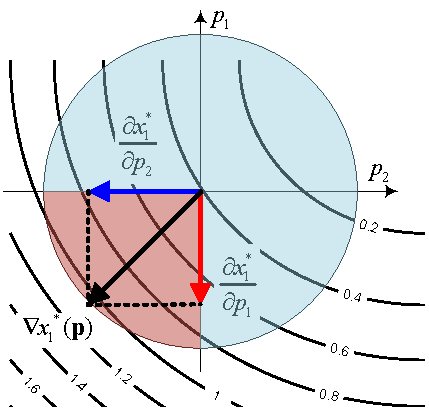
\includegraphics[width=0.4\textwidth]{5a_parameter_demo_ge0}
	\caption{Isocontours of the response surface ${x_1}^*(\mathbf{p})$ and transition rule $\mathbf{N}~\mathbf{J}^{\text T}(\mathbf{p})\mathbf{M} \ge \mathbf{0}$ in a two-dimensional parameter space}
	\label{fig:contourdemo}
\end{figure}

To illustrate Equation~(\ref{eq:transitionrulematrix}), a two-dimensional parameter space example is shown in Figure~\ref{fig:contourdemo}. 

The change agent vector $\mathbf{n}$ describes a quadrant (or hyper-octant in higher dimensions) in the parameter space that should contain the gradient vector $\nabla\hat{\mathbf{x}^*}(\mathbf{p})$. The sign of the gradient vector is modified by the monotonicity vector $\mathbf{m}$. Figure~\ref{fig:contourdemo} shows an example when $m_l\nabla\hat{{x_1}^*}(\mathbf{p}) \ge 0$ and lies within the quadrant defined by $\mathbf{n}$. Designs within the change agent quadrant and having gradients leading to an increase in their value are considered scalable.

In order to map scalable designs from the parameter space to the design space, the design space is resampled randomly and the transition rule (Equation~(\ref{eq:transitionrulematrix})) is checked for every sample $\mathbf{p}_o$. If $\mathbf{N}~\mathbf{J}^{\text T}(\mathbf{p}_o)\mathbf{M} \ge \mathbf{0}$ is satisfied then the corresponding design $\hat{\mathbf{x}^*}(\mathbf{p}_o)$ is retrieved and appended to a set of scalable solutions $\mathbf{X}_s$.

The procedure for obtaining the set of scalable optimal solutions is presented in Algorithm~\ref{algo:SODalgo}.

\begin{algorithm}
	\DontPrintSemicolon % Some LaTeX compilers require you to use \dontprintsemicolon instead
	\KwIn{
		Parameter space bounds $\mathbf{L}_p$ and $\mathbf{U}_p$, \ac{KS} response surface of parameter space $\hat{\mathbf{x}^*}(\mathbf{p})$, Jacobian of parameter space $\nabla\hat{\mathbf{x}^*}(\mathbf{p})$, Monotonicity matrix $\mathbf{M}$, Change agent matrix $\mathbf{N}$, \ac{LH} samples of parameter space $\left[\mathbf{p}_{1},\mathbf{p}_{2}, \cdots, \mathbf{p}_{o}\right]^{\text T}$
	}
	\KwOut{$\mathbf{X}_s$}		
	\For{$k \gets 1$ to $o$} {
		%				Populate possible points using LH and store them in $S_k$\;
		%				Update the RAM using built SM\;

		\If{$\mathbf{N}~\mathbf{J}^{\text T}(\mathbf{p}_k)\mathbf{M} \ge \mathbf{0}$} {
			Find design variables corresponding to parameters sample using response surface $\mathbf{x}^*(\mathbf{p}_k) = \hat{\mathbf{x}^*}(\mathbf{p_k})$\;
			Augment $\mathbf{X}_s \gets \mathbf{X}_s \cup \{ \mathbf{x}^*(\mathbf{p}_k) \} $\;
		}
		\Else{
			$\mathbf{X}_s \gets \mathbf{X}_s$\;
		}
	}
	\caption{Pseudo-algorithm for obtaining the set of scalable optimal designs $\mathbf{X}_s$}
	\label{algo:SODalgo}
\end{algorithm}

% --------------------------------- Numerical example ------------------------------------ %
\subsection{Numerical example for determining the scalable design set} \label{subsec:numex}

\begin{figure*}[h!]
	\centering
	\subfloat[Sampling effect \label{fig:nsamples_test}]{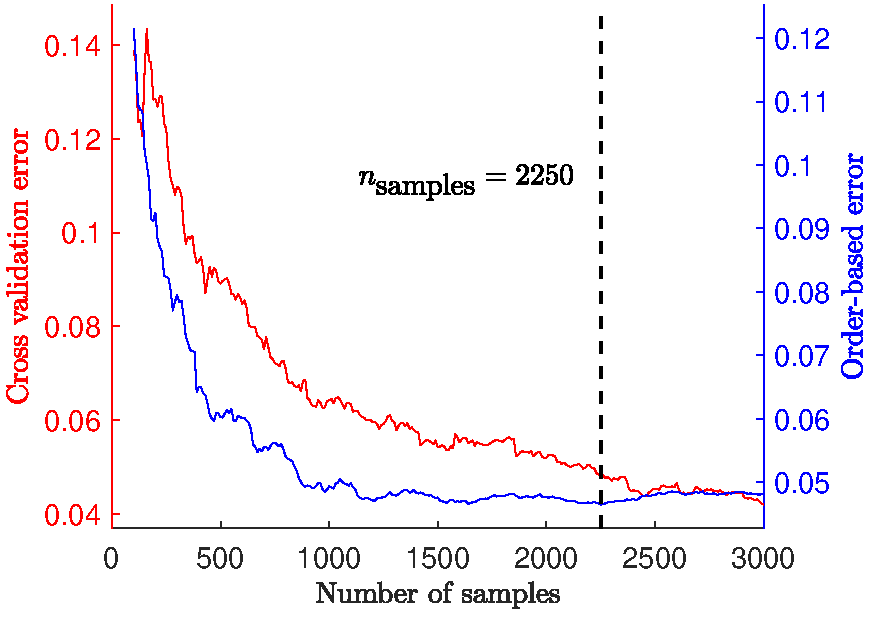
\includegraphics[width=0.4\textwidth]{OE_nsamples}} \hspace{0.07\textwidth}%
	\subfloat[Bandwidth effect \label{fig:bandwidth_test}]{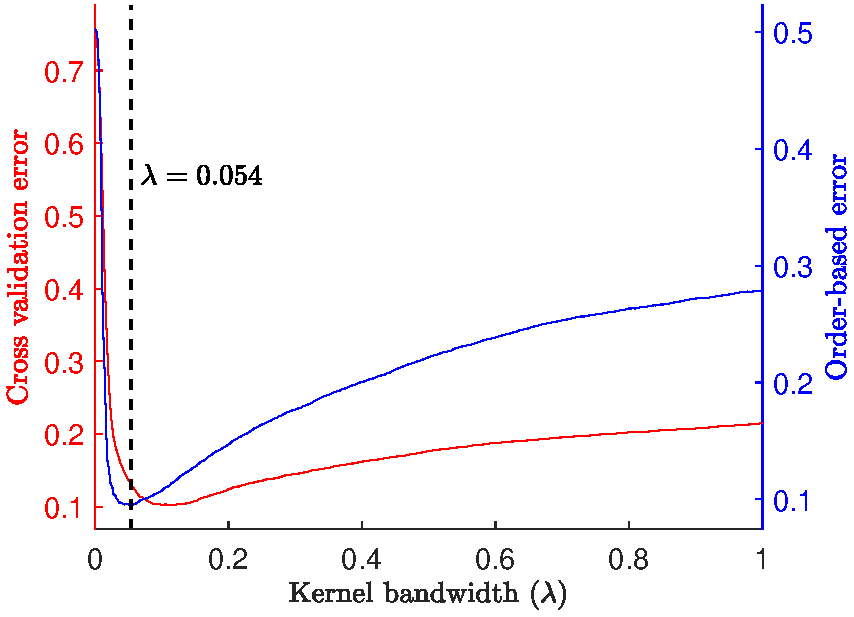
\includegraphics[width=0.4\textwidth]{OE_bandwidth}}
	\caption{Effect of number of training points and kernel bandwidth on order-based error}
	\label{fig:HPeffect}
\end{figure*}

\begin{figure*}[h!]
	\centering
	\subfloat[Test function \label{fig:testfunanalytical}]{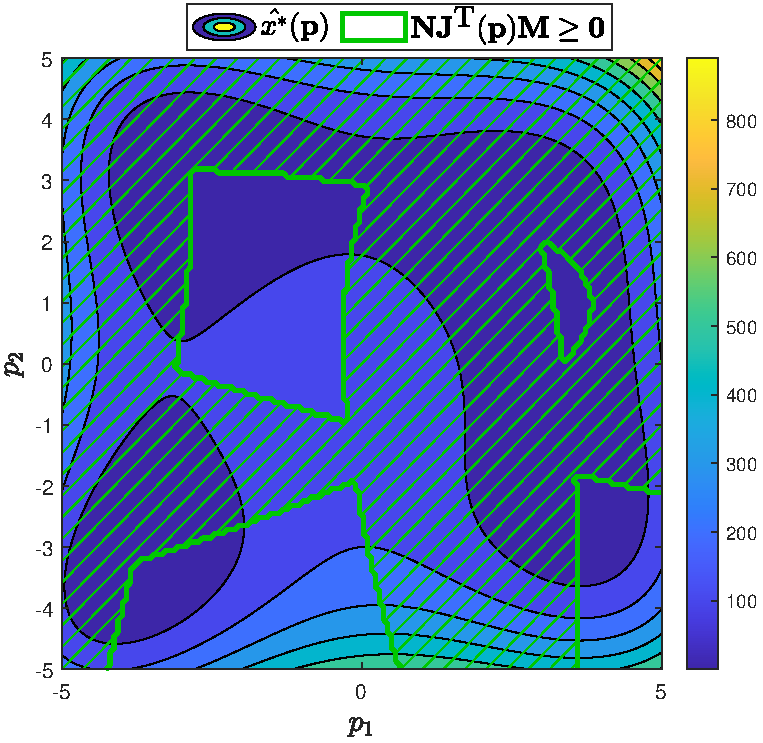
\includegraphics[width=0.4\textwidth]{test_problem}} \hspace{0.07\textwidth}%
	\subfloat[\ac{KS} approximation \label{fig:testfunKS}]{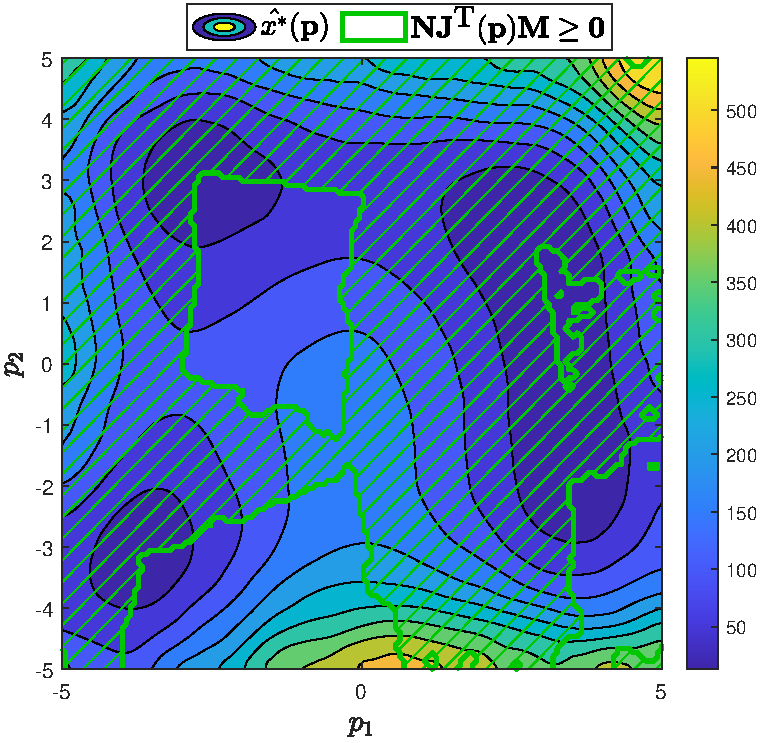
\includegraphics[width=0.4\textwidth]{test_problem_KS}}	
	\caption{Approximation of scalable set using \ac{KS} with non-scalable regions of the parameter space hatched}
	\label{fig:testfun}
\end{figure*}

We demonstrate the concepts related to constructing a \ac{KS} response surface to estimate the Jacobian using a numerical example. We also show how the estimated Jacobian can be used for identifying the scalable design set. Himmelblau's test function is used as it features multiple local minima. The test function and its Jacobian are
\begin{displaymath}
%	\begin{aligned}
		{x}^*(p_1,p_2) = ({p_1}^{2}+{p_2}-11)^{2}+({p_1}+{p_2}^{2}-7)^{2} 
		\end{displaymath}
		and
	\begin{displaymath}	
		\mathbf{J}(p_1,p_2) = \begin{bmatrix}
			4{p_1}({p_1}^2 + {p_2} - 11) + 2({p_1} + {p_2}^2 -7) \\ 
			2({p_1}^2 + {p_2} - 11) + 4{p_2}({p_1} + {p_2}^2 -7) 
	\end{bmatrix},
	\end{displaymath}
	respectively.% (i.e., $\mathbf{p} = \left[p_1,p_2\right]$).

We approximate the response surface for this function via \ac{KS} to obtain $\hat{{x}^*}(\mathbf{p)}$. For this example we set the change agent vector as $\mathbf{n} = \left[1~-1\right]$ and the monotonicity vector as $\mathbf{m} = \left[1\right]$. The test function is sampled via \acp{LH} to create the training data for the \ac{KS} model. We evaluate the transition rule $\mathbf{N}~\mathbf{J}^{\text T}(\mathbf{p})\mathbf{M} \ge \mathbf{0}$ defining the scalable set using the analytical and estimated Jacobian. The estimated Jacobian was obtained by differentiation of the \ac{KS} basis functions. A portion of the \ac{LH} samples are reserved for use as a validation set and are not used to train the \ac{KS} model. The cross-validation error reflects the classification accuracy of the \ac{KS} response surface at the validation points as part of the true scalable set obtained from the analytical Jacobian.

In addition, we use the order-based error proposed in \cite{Audet2018} since it does not rely on comparisons with the true scalable set (which is not available in real problems). It is computed by checking how accurately the response surface model orders the validation points. It is calculated as 
%
\begin{equation}
    \label{eq:oeobjective}
	\varepsilon_{OE} = \frac{1}{n_{cv}^2} \sum_{i=1}^{n_{cv}} \sum_{l=1}^{n_{cv}} \theta\left(\mathbf{x}^*(\mathbf{p}_i) - \mathbf{x}^*(\mathbf{p}_l),\hat{\mathbf{x}^*}(\mathbf{p}_i) - \hat{\mathbf{x}^*}(\mathbf{p}_l)\right),
\end{equation}
%
where $n_{cv}$ is the number of validation points. The function $\theta$ is defined as
%
\begin{equation}
    \label{eq:theta}
    \theta\left(a,b\right) = \left(a \le 0\right)~\textrm{xor}~\left(b \le 0\right),
\end{equation}
%
where xor is the logical \textit{exclusive or} operator.
Figure~\ref{fig:HPeffect} shows the effect of the number of training points ($n_{\textrm{samples}}$) and the bandwidth ($\lambda$) on the cross validation and order-based errors.

It can be seen that there is a unique combination of $n_{\textrm{samples}}$ and $\lambda$ that yield the best response surface for assessing scalability in the parameter space. The true and estimated scalable sets are shown in Figure~\ref{fig:testfun}. The \ac{KS} model used for the estimation is trained using 2305 training samples and a bandwidth of $\lambda = 0.054$.
Figure~\ref{fig:testfun} shows that \ac{KS} is capable of capturing the scalable set despite underestimating the magnitude of the test function. Figure~\ref{fig:HPeffect} shows that the order-based error is a good indication of the prediction accuracy of the \ac{KS} model for the scalable set. As a result, the \ac{KS} parameters and number of training points can be determined by minimizing the order-based error.

In summary, the proposed methodology consists of two design filters that determine a set of scalable optimal designs to be considered for further development. The first filter retains designs that dominate in terms of performance throughout the parameter space (set of parametric optimal designs $\mathbf{X}^*$). The second filter retains designs that are scalable by remanufacturing (scalable design set $\mathbf{X}_s$). The number of samples for the \ac{KS} response surface is chosen such that the order-based error is minimized with respect to a validation set. The methods developed in this section are demonstrated using the application example.

The proposed methodology, is presented as a flow diagram in Figure~\ref{fig:SBDmethods}

\begin{figure}[h]
	\centering
	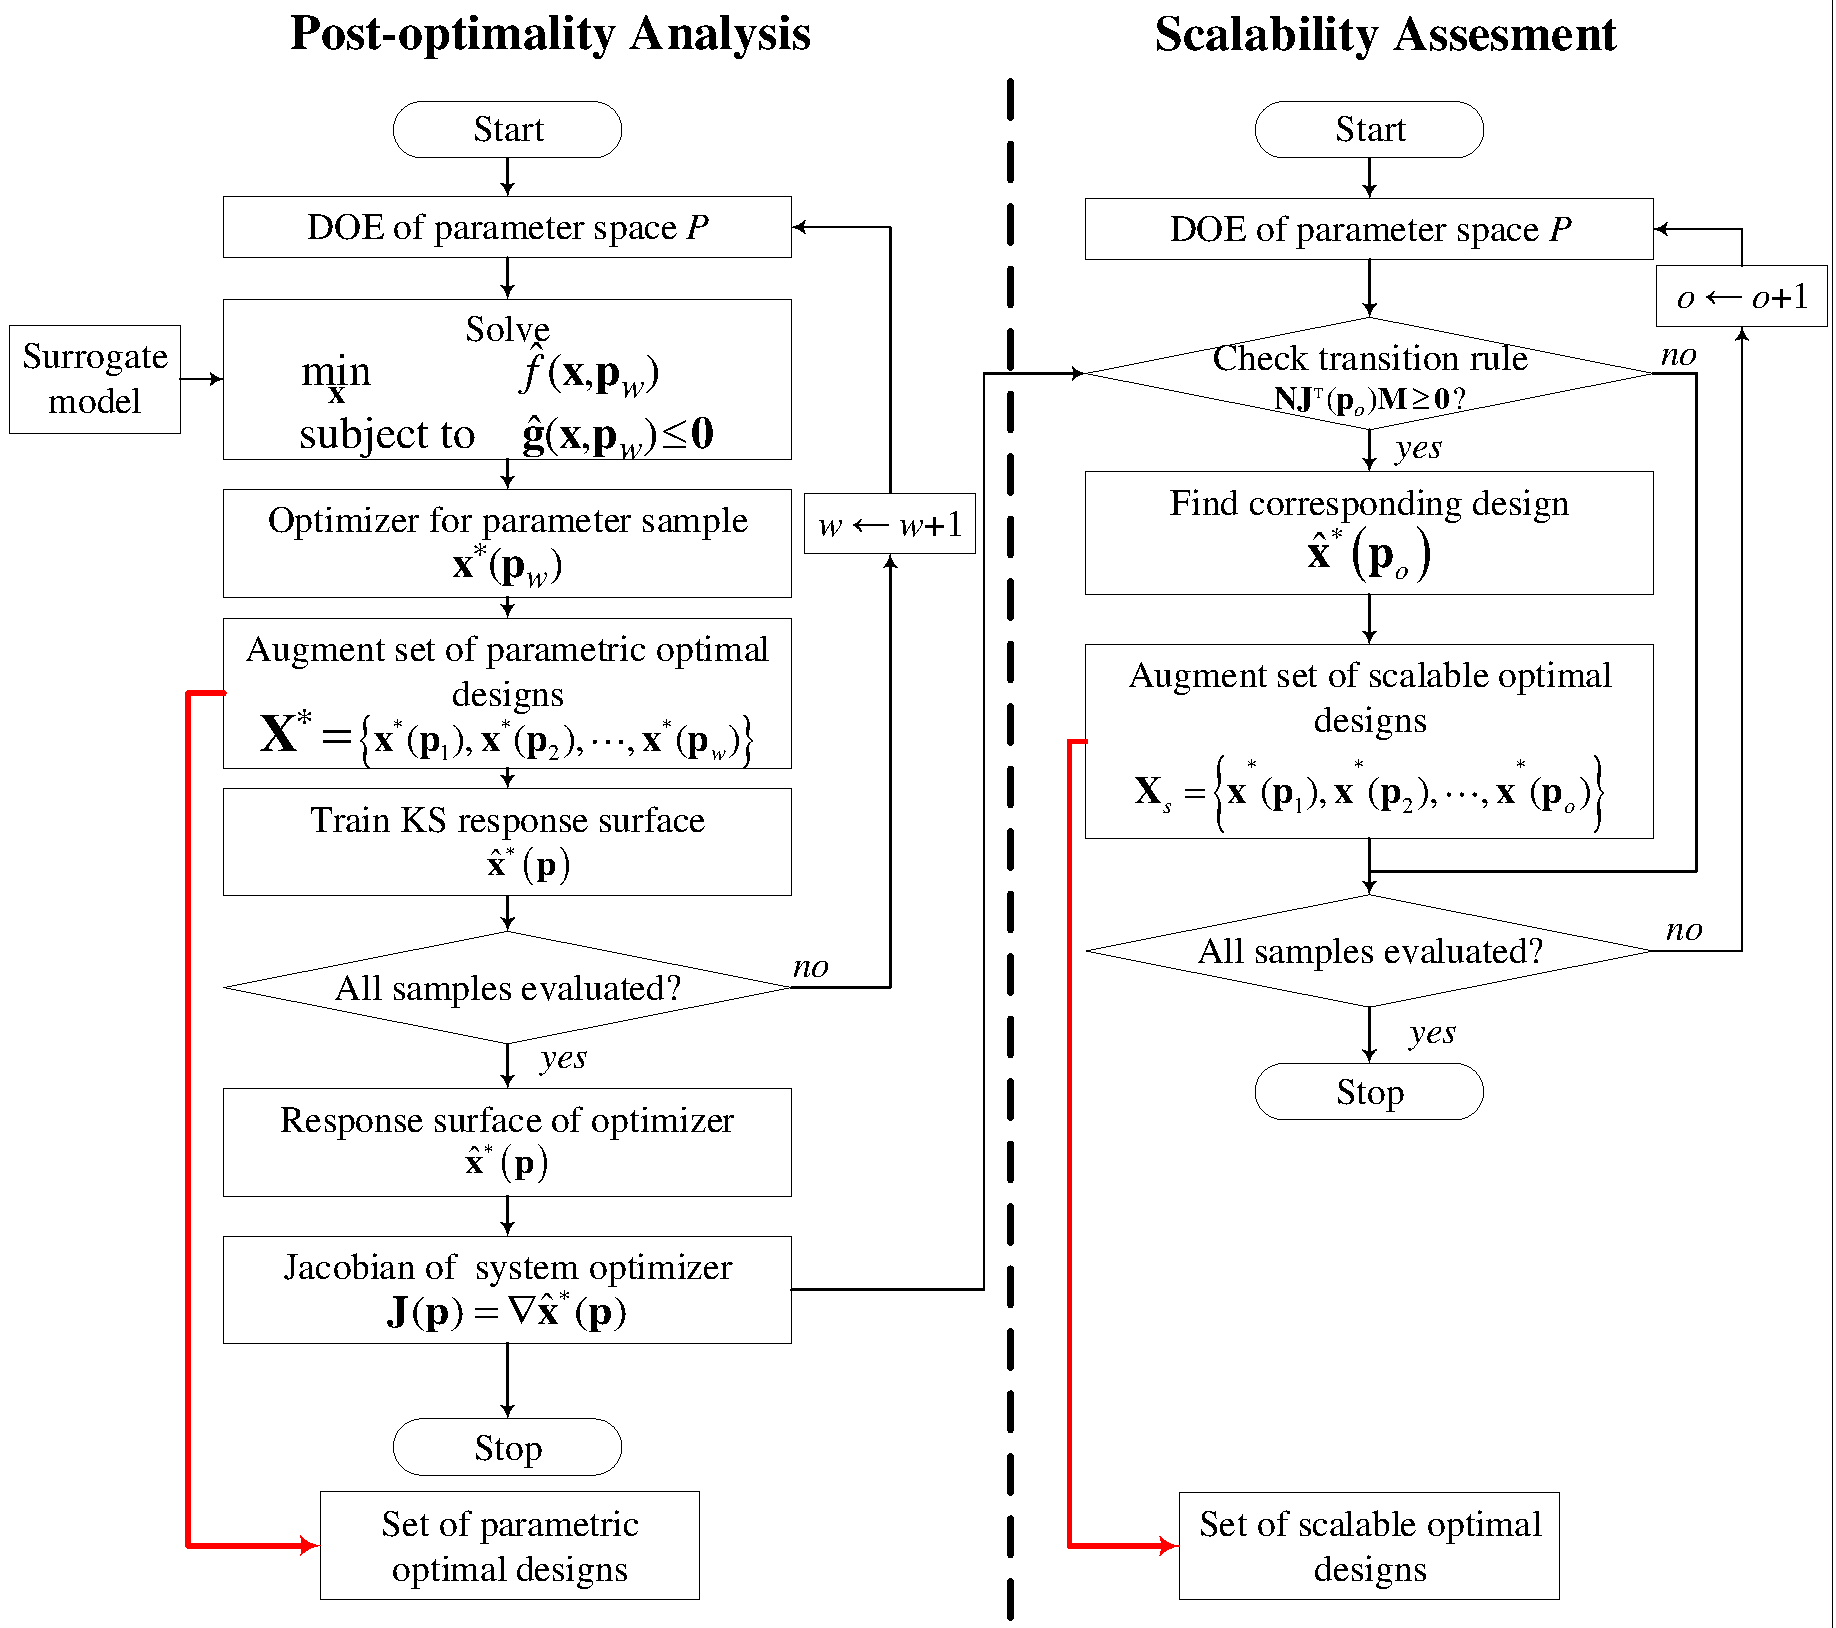
\includegraphics[width=.95\textwidth]{5_methodology_V2.pdf}
	\caption{ \label{fig:SBDmethods} Set-based design space reduction methodology}
\end{figure}

%=========================== APPLICATION EXAMPLE ===============================%
\section{Application example: aeroengine component remanufacturing} \label{sec:SBDusecase}

The \ac{TRS} structural aeroengine component described in Chapter~\ref{ch:thermomechanical} is used to demonstrate the methodology for obtaining scalable optimal designs when considering it for remanufacturing.

The safety factor against low-cycle fatigue is computed using the model in Section~\ref{subsec:fatigueanalysis} as a structural performance requirement.

% Model summary
The design variables for this problem shown in Figure~\ref{fig:TRSoverview} are extracted from Table~\ref{table:modelinputs} and listed in Table~\ref{table:SBDvariables} along with their monotonicity.

\begin{table}[h!]
\centering
\renewcommand{\arraystretch}{1.0}% Wider
\footnotesize\addtolength{\tabcolsep}{-5pt}
\caption{Design variables ${\textbf{x}}$}
\label{table:SBDvariables}
	\begin{tabular}{lcc>{\centering\arraybackslash}p{1cm}>{\centering\arraybackslash}p{1cm}>{\centering\arraybackslash}p{1cm}}
		\hline\hline
		\bf Design variable & \bf Notation & \bf Units & \bf Lower bound & \bf Upper bound & \bf Mono- tonicity\\
		\hline
		Stiffener axial position & $x_1$ & mm & 37 & 145 & 0 \\
		Stiffener thickness  & $x_2$ & mm & 2 & 10 & 1 \\
		Stiffener width & $x_3$ & mm & 10 & 40 & 1  \\
		Laser Power & $P_{\textrm{laser}}$ & W & 3,500 & 4,000 & 0\\ 
		%Laser beam radius & ${r_l}$ & mm & 12.6 & 16.0 \\ 
		%Scanning speed& ${V}$ & mm/s & 4.0 & 4.6 \\ 
		\hline\hline
	\end{tabular}
\end{table}

Similarly, the design parameters relevant to the problem in this chapter are extracted from Table~\ref{table:modelinputs} and are listed in Table~\ref{table:SBDparametervar} along with their change agent values.

\begin{table}[h!]
\centering
\renewcommand{\arraystretch}{1.0}% Wider
\footnotesize\addtolength{\tabcolsep}{-5pt}
\caption{Design parameters $\textbf{p}$}
\label{table:SBDparametervar}
\begin{tabular}{lcc>{\centering\arraybackslash}p{2cm}>{\centering\arraybackslash}p{1cm}}
\hline\hline
\bf Parameter    & \bf Notation & \bf Units & \bf Range  &\bf Change agent\\ \hline
Internal pressure load  & ${P}_{\textrm{load}}$ & MPa & $2 \pm 0.5$ & 1\\ 
Deposit melting point & $T_m$ & $^o$C & $1,500 \pm 100$ & -1\\
Substrate base width & $W_{\textrm{total}}$ & mm & $137.5 \pm 17.5$ & -1\\
\hline\hline
\end{tabular}
\end{table}

The remanufacturing model variables and parameters given by Tables~\ref{table:SBDvariables} and \ref{table:SBDparametervar} respectively are used for the formulation of the optimization problem for \ac{SBD} in the following section. 

% --------------------------- parametric optimal design space reduction ------------------------------ %
\subsection{Problem formulation} \label{subsec:SBDproblemformulation}

The design optimization problem is formulated as 
\begin{equation}
	\label{eq:SBCEopt}
	\begin{aligned}
		& \min_{\mathbf{x} = \left[x_1,x_2,x_3,P_{\textrm{laser}}\right]^{\text T}}
		& & f(\mathbf{x};\mathbf{p}) = -n_{\textrm{safety}}(P_{\textrm{load}})\\
		& \text{subject to}
		& & g_1(\mathbf{x};\mathbf{p}) = x_3 + x_1 - W_{\textrm{total}} \le 0\\
		& & & g_2(\mathbf{x};\mathbf{p}) = T_m - T_\textrm{deposit} \le 0,
		% & & & g_3(\mathbf{x}) = U_{\textrm{res}}(\mathbf{x}) - U_{\textrm{max}} \le 0\\
%		& \text{where}
%		& & \mathbf{x}^{\text T} = \left[x_1,x_2,x_3,P\right]
	\end{aligned}
\end{equation}
where $n_{\textrm{safety}}$ is the safety factor against low cycle fatigue or first cycle yielding for the load case. The constraints pertain to the substrate width on the outer casing (the region where deposition is permitted) and the melting temperature of the deposit material needed to consolidate the material.

% --------------------------- Design space reduction to parametric optimal design set ------------------------------ %
\subsection{Parametric optimal design results} \label{subsec:reduceddesignspace}

The design optimization problem in Equation~(\ref{eq:SBCEopt}) is solved using the \ac{MADS} algorithm. We use the \texttt{OrthoMADS} implementation provided by the \texttt{NOMAD} algorithm \cite{LeDigabel2011}. The termination criterion for \ac{MADS} was the minimum mesh size (defined by Audet and Dennis \cite{Audet2006a}) reached in the virtually discretized design variable space. Non-opportunistic latin hypercube search was used during the search step. A progressive barrier approach was used for handling constraints \cite{Audet2009}. This choice of algorithm is motivated by the possible non-existence of gradients or the inability to approximate them with reasonable computational cost and warranted due to its rigorous convergence properties.

As described earlier, \acp{LH} are used to sample the design and parameter spaces defined by the bounds and ranges of the design variables and parameters, respectively (see Tables 
~\ref{table:SBDvariables} and \ref{table:SBDparametervar}).

For our numerical investigations, the design optimization problem is solved for 1200 \ac{LH} samples of the parameter space to obtain a set of parametric optimal design solutions. Up to 900 samples are used as a training set for the \ac{KS} model, while the remaining 300 are reserved for use as a validation set to check the order-based error.

The effect of the parameters on the optimizer is illustrated by 3 sample results shown in Figure~\ref{fig:SBD1sens2P1} (see Table~\ref{table:optresults}).

\begin{figure*}%[t]
	\centering
	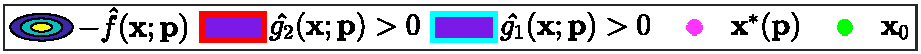
\includegraphics[width=0.65\textwidth]{9_f1_legend} \vspace{-0.02\textwidth}\\
	\subfloat[$\mathbf{p}_1$ \label{fig:p1}\label{fig:9a}]{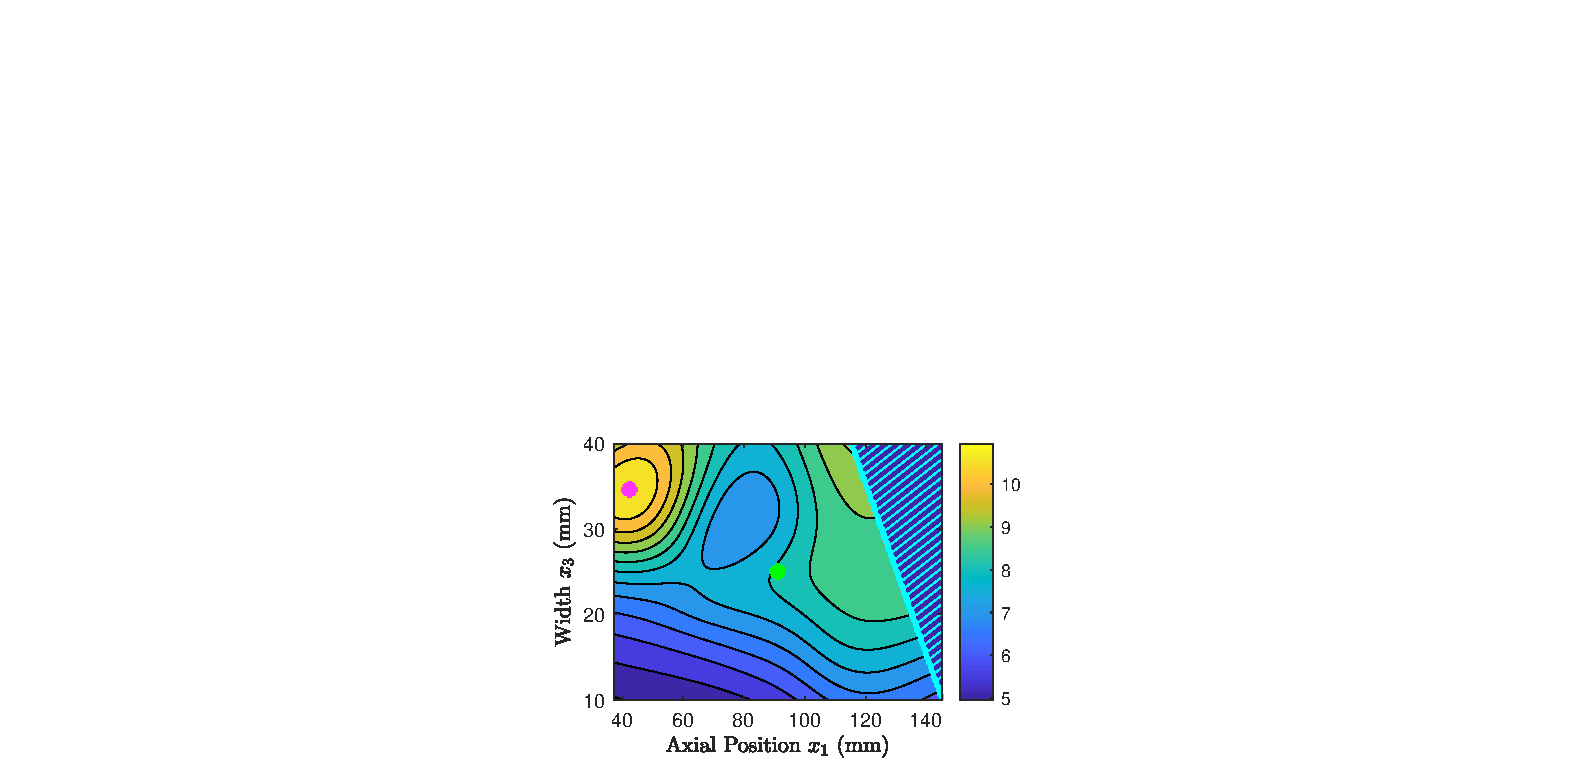
\includegraphics[height=0.21\textwidth]{9a_f1_1_p1}} \hspace{0.03\textwidth}%
	\subfloat[$\mathbf{p}_2$ \label{fig:p2}\label{fig:9b}]{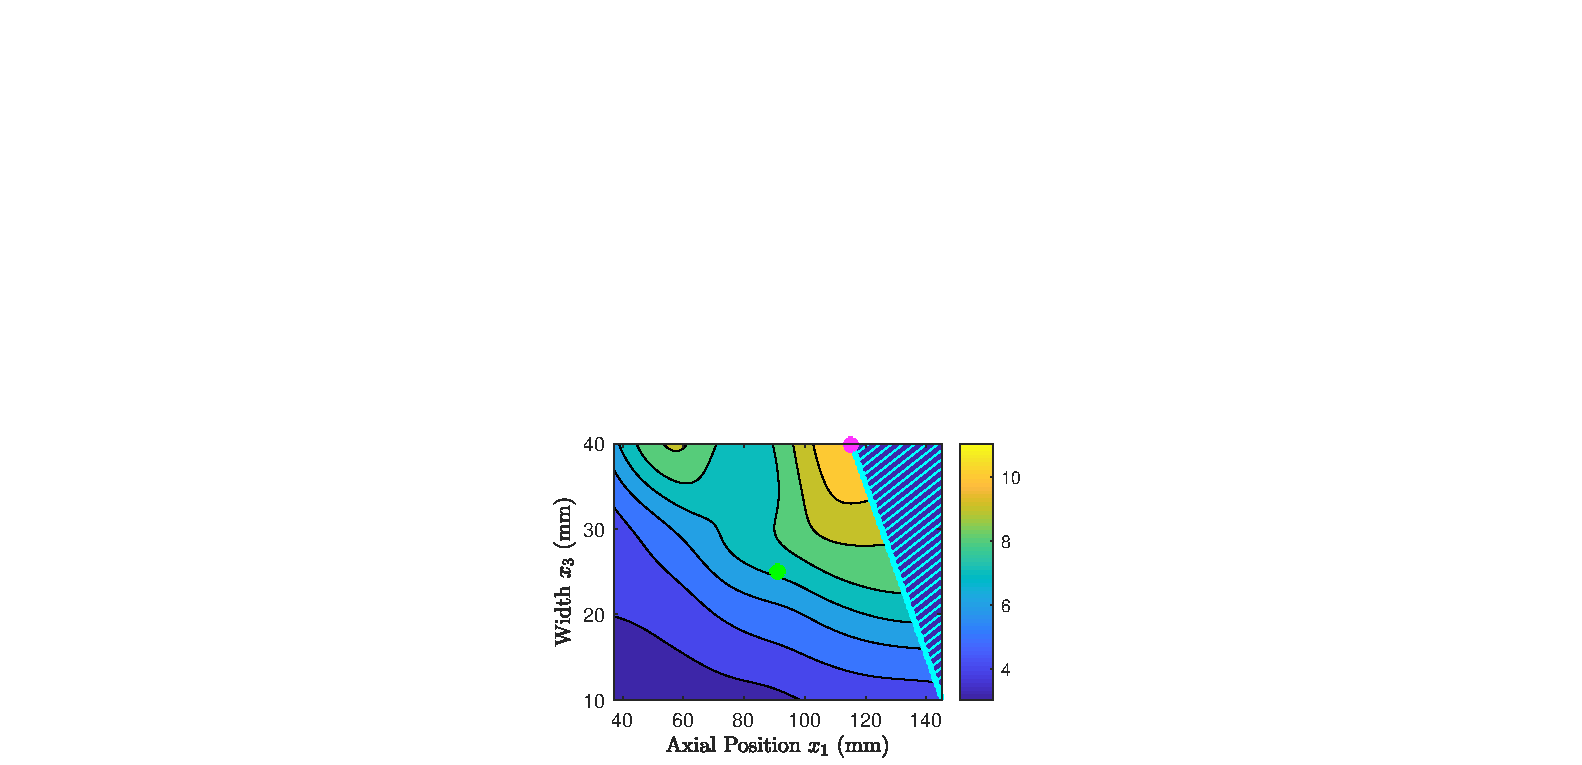
\includegraphics[height=0.21\textwidth]{9b_f1_1_p2}} \hspace{0.03\textwidth}%
	\subfloat[$\mathbf{p}_3$ \label{fig:p3}\label{fig:9c}]{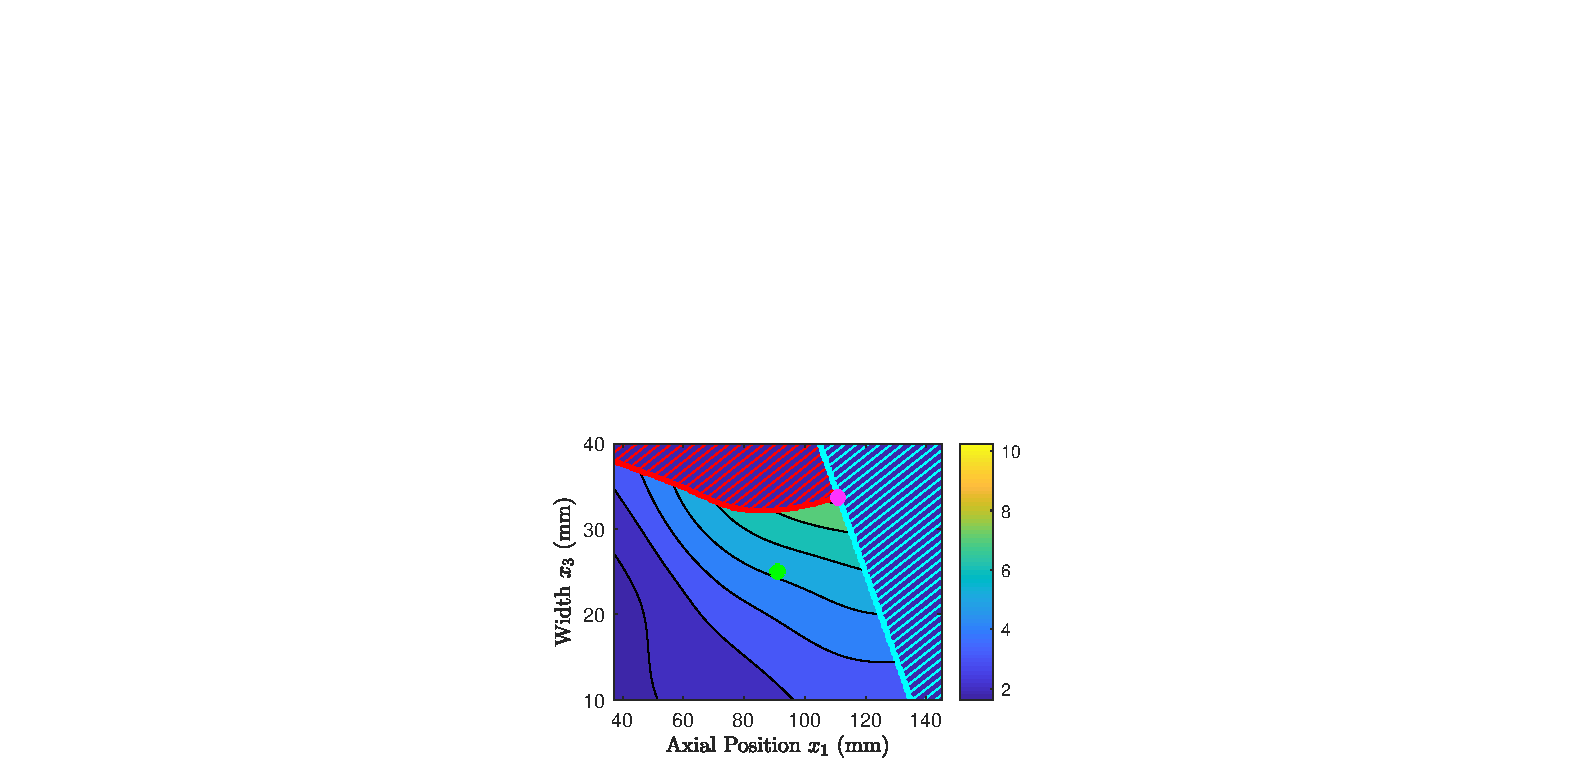
\includegraphics[height=0.21\textwidth]{9c_f1_1_opt}}
	\caption{Three sample parametric optimal designs; $x_0$ denotes the baseline design}
	\label{fig:SBD1sens2P1}
\end{figure*}
\begin{table*}[h!]
\centering
\renewcommand{\arraystretch}{1.0}% Wider
\small\addtolength{\tabcolsep}{-5pt}
\caption{Sample optimization problem results}
\label{table:optresults}
\begin{tabular}{cC{1.2cm}C{1.2cm}C{1.2cm}C{1.2cm}|C{1.2cm}C{1.2cm}C{1.2cm}|C{1.2cm}C{1.2cm}C{1.2cm}}
\toprule\toprule
\multirow{5}{1cm}{\textbf{Result}} & \multirow{5}{1cm}{\centering\textbf{Units}} & \multicolumn{9}{c}{\textbf{Parameters}}\\ \cline{3-11}
 & & \multicolumn{3}{c}{$\mathbf{p}_1$} & \multicolumn{3}{c}{$\mathbf{p}_2$} & \multicolumn{3}{c}{$\mathbf{p}_3$} \\ \cline{3-11}
 & & ${P}_{\textrm{load}}$ & $T_m$ & $W_{\textrm{total}}$ &  ${P}_{\textrm{load}}$ & $T_m$ & $W_{\textrm{total}}$ &  ${P}_{\textrm{load}}$ & $T_m$ & $W_{\textrm{total}}$ \\
 & & (MPa) & ($^o$C) & (mm) & (MPa) & ($^o$C) & (mm) & (MPa) & ($^o$C) & (mm) \\
 & & 1.87 & 1,400 & 155 &2.08 & 1,400 & 155 &  2.3973 & 1,427 & 145 \\
\hline
$x_1^*$ & mm & \multicolumn{3}{c|}{42.2} & \multicolumn{3}{c|}{115.1} & \multicolumn{3}{c}{110.9}\\
$x_2^*$ & mm & \multicolumn{3}{c|}{10.0} & \multicolumn{3}{c|}{9.0} & \multicolumn{3}{c}{8.8}\\
$x_3^*$ & mm & \multicolumn{3}{c|}{34.7} & \multicolumn{3}{c|}{39.9} & \multicolumn{3}{c}{33.7}\\
${P_{\textrm{laser}}}^*$ & W & \multicolumn{3}{c|}{3,500} & \multicolumn{3}{c|}{3,770} & \multicolumn{3}{c}{3,991}\\
$g_1(\mathbf{x}^*)$ & mm & \multicolumn{3}{c|}{-78.1} & \multicolumn{3}{c|}{0 (active)} & \multicolumn{3}{c}{0 (active)}\\
$g_2(\mathbf{x}^*)$ & $^o$C & \multicolumn{3}{c|}{-393} & \multicolumn{3}{c|}{-381} & \multicolumn{3}{c}{0 (active)}\\
$f(\mathbf{x}^*)$ & - & \multicolumn{3}{c|}{-11} & \multicolumn{3}{c|}{-11} & \multicolumn{3}{c}{-8}\\
\toprule\toprule
\end{tabular}
\end{table*}
These 3 samples have been chosen to include one interior optimal design (Figure~\ref{fig:9a}), one boundary optimal design with one active constraint ((Figure~\ref{fig:9b}), and one boundary optimal design with two active constraints (Figure~\ref{fig:9c}).
The optimizers obtained by sampling the parameter space are used to construct a convex hull to quantify the size of the set of parametric optimal designs. The \texttt{qhull} algorithm was used to construct the 4-dimensional polygon (polytope) characterizing the convex hull \cite{Barber2002}.

% --------------------------- Scalable Design Space ------------------------------ %
\subsection{Scalable optimal design results} \label{subsec:scalabledesignspace}

Of the 900 parametric optimal designs obtained by solving the optimization problem for different parameter values, 592 samples were used to construct a response surface that can predict a parametric optimal design for other parameter values. As explained in Section~\ref{subsec:numex} the order-based error relative to a validation set was minimized to determine the number of training samples. The kernel bandwidth ($\lambda$) was determined to be 0.71. This result is shown in Figure~\ref{fig:HPeffectSBD}.

Designs meeting scalability requirements in the parameter space are identified using the scalability constraint in Section~\ref{subsec:SBDfAM}. The monotonicity vector is defined as $\mathbf{m} = [0~1~1~0]^{\text T}$ for the variables in Table~\ref{table:SBDvariables}. The {change agent} vector is defined as $\mathbf{n} = [1~-1~-1]^{\text T}$. As an illustrative example, the two-dimensional projections of the parameter space for the optimal width design variable are depicted in Figure~\ref{fig:parameterspacescaled}.
\begin{figure*}%[t]
	\centering
	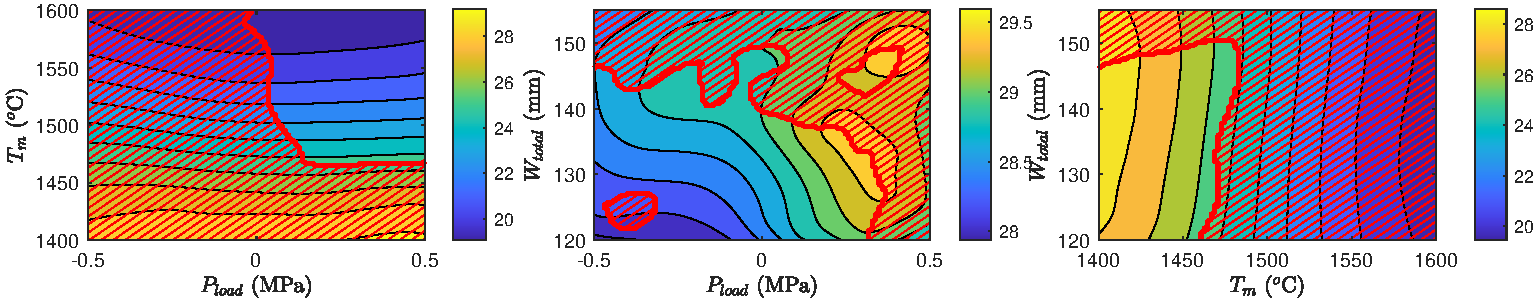
\includegraphics[width=1\textwidth]{12_parameter_space_scaled_V2.pdf} %12_parameter_space_scaled.pdf
	\caption{ \label{fig:parameterspacescaled} Projections of the optimal width design variable $\hat{x_3}^{*}$ with non-scalable regions of the parameter space hatched}
\end{figure*}
\begin{figure*}[h!]
	\centering
	\subfloat[Sampling effect \label{fig:nsamples}]{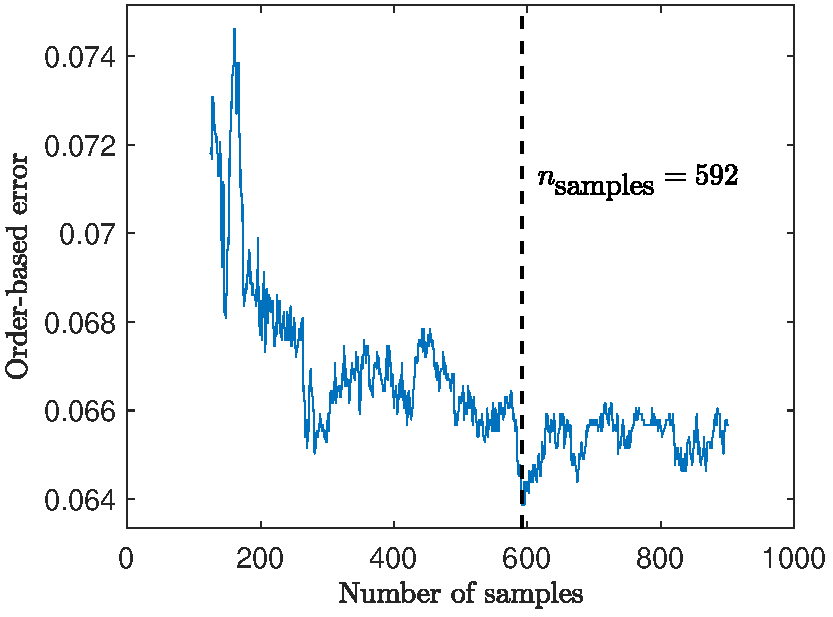
\includegraphics[width=0.4\textwidth]{OE_nsamples_SBD}} \hspace{0.02\textwidth}%
	\subfloat[Bandwidth effect \label{fig:bandwidth}]{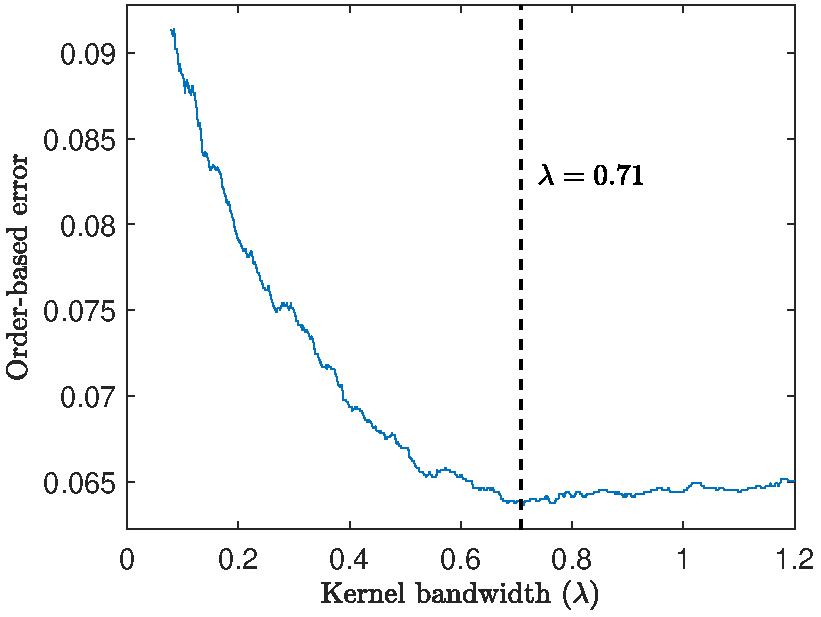
\includegraphics[width=0.4\textwidth]{OE_bandwidth_SBD}}	
	\caption{Effect of number of training points and kernel bandwidth on order-based error}
	\label{fig:HPeffectSBD}
\end{figure*}

The scalability transition rule results in pockets within the parameter space that can be mapped back to design space by evaluating the optimizer response surface within these pockets. The parameter space is sampled using a full factorial grid and designs meeting the scalability constraint are tabulated and projected on the design space in Figure~\ref{fig:FullM}.
\begin{figure*}[h!]
	\centering
	\subfloat[$\mathbf{m} = [0~1~1~0{]}^{\text T}$, $\mathbf{n} = [1~-1~-1{]}^{\text T}$ \label{fig:FullM}]{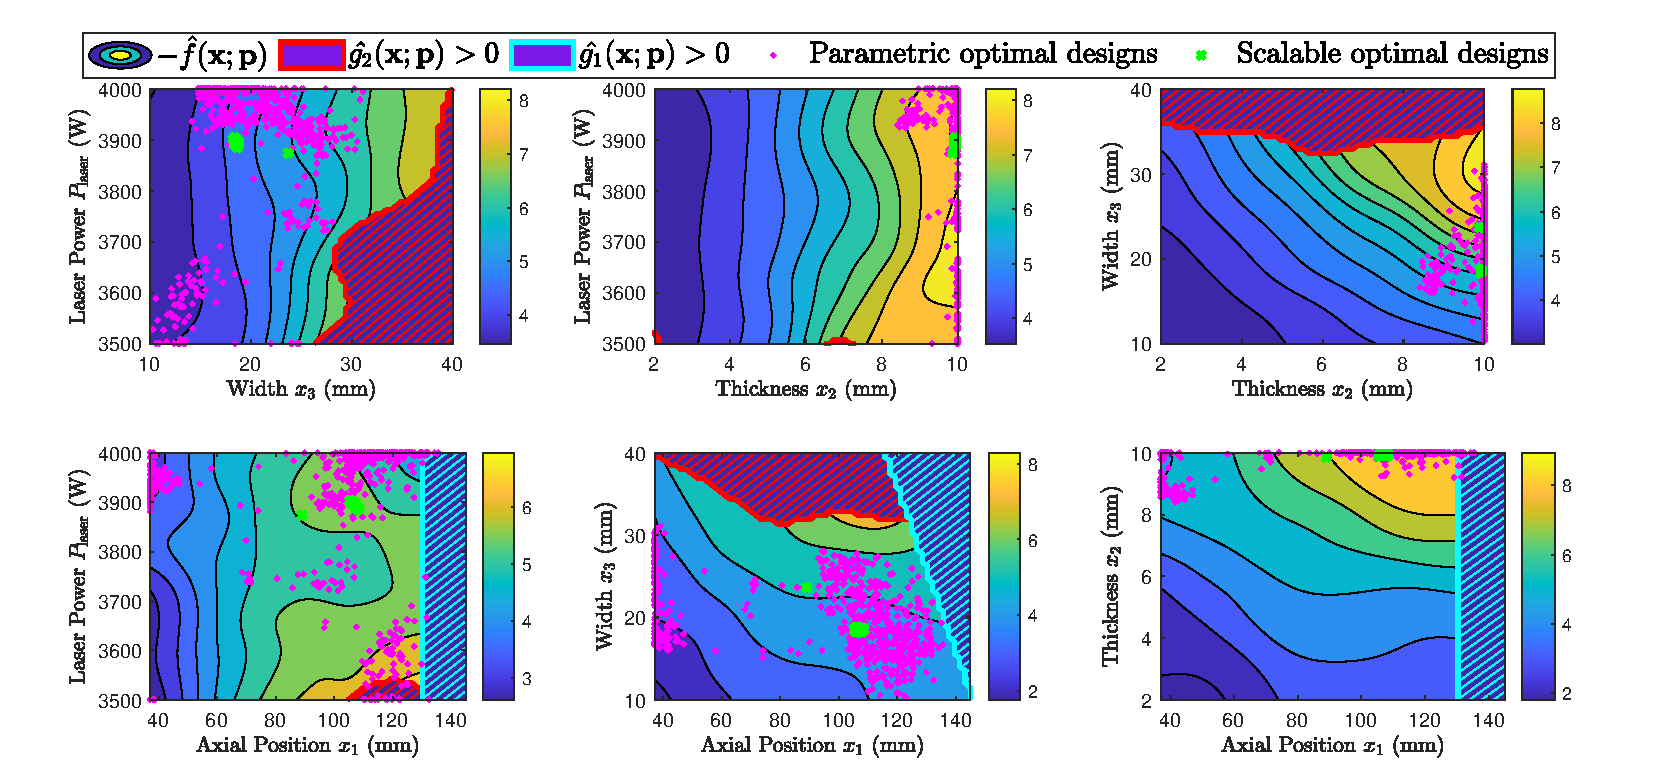
\includegraphics[width=1\textwidth]{8_design_space_V3.pdf}}\\
	\subfloat[$\mathbf{m} = [0~0~1~0{]}^{\text T}$, $\mathbf{n} = [1~-1~-1{]}^{\text T}$ \label{fig:RelaxedM}]{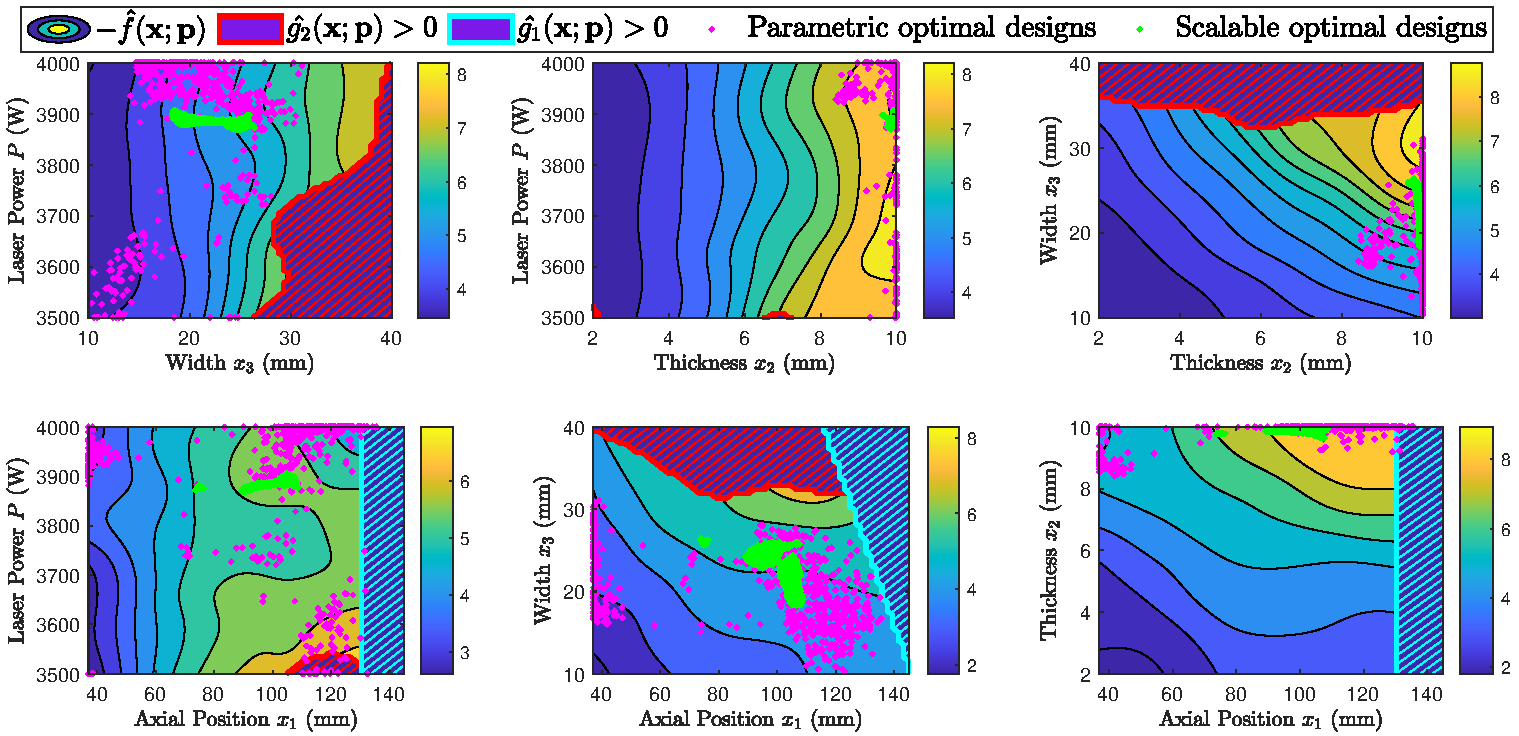
\includegraphics[width=1\textwidth]{8_design_space_V4.pdf}}	
	\caption{Safety factor in the feasible design space as a function of design variables for different monotonicity vectors}
	\label{fig:designspace}
\end{figure*}

The convex hull formed by the scalable optimal designs is considerably smaller in volume than that formed by the set of parametric optimal designs.

 The set of scalable optimal designs can be enlarged to include more designs by relaxing some of the scalability constraints. We relax all the constraints with respect to the thickness design variable $x_2$ by setting the monotonicity with respect to $x_2$ to $0$. The monotonicity vector becomes $\mathbf{m} = [0~0~1~0]^{\text T}$. The result of this relaxation is shown in Figure~\ref{fig:RelaxedM}.

Adhering to scalability constraints allows designers the flexibility to scale designs as parameters evolve even after commitment by considering remanufacturing scenarios. Figure~\ref{fig:parameterspacescaled} shows this scenario as the contours of $\hat{x_3}^{*}$ increase in value for any vector contained within the change agent hyperoctant as defined by $\mathbf{n}$.

% --------------------------- Design space variability ------------------------------ %
\subsection{Design set variability and comparison} \label{subsec:dspacevar}

Having generated the feasible design set, the set of parametric optimal designs, and the set of scalable optimal designs for the \ac{TRS} remanufacturing problem, some comparisons can be made.
Several metrics exist in the literature for comparing the variability of a design solution set generated by parametric optimal design tools such as those formulated in this thesis. The volume of the convex hull provides a good perception of design variability provided that there are sufficient points to construct the polytope characterizing the convex hull \cite{Brown2019}. The convex hull volume was used to compare the reduction in the design sets as our methodology was applied to the \ac{TRS} problem. The lower and upper bounds (LB and UB, respectively) of the ranged set containing each solution set are also found. They are used to compute the volume of the bounding hyper-rectangle. The hyper-rectangle volume provides a benchmark against the ranged set representation used for previous \ac{SBD} studies \cite{Qureshi2014, Nahm2005, Olewnik2004,Liu2008,Suh2007}.

% Case with one active variable
\begin{table*}[h!]
	\centering
	\small\addtolength{\tabcolsep}{-5pt}
	\caption{Design space comparison results}
	\label{table:designvariability}
	\begin{tabular}{l|C{1.2cm}C{1.2cm}|C{1.2cm}C{1.2cm}|C{1.2cm}C{1.2cm}|C{1.2cm}C{1.2cm}}
		\toprule\toprule
		\multirow{2}{1cm}{\textbf{Quantity}} & \multicolumn{2}{c|}{Feasible design} & \multicolumn{2}{c|}{Set of parametric} & \multicolumn{4}{c}{Scalable design set}\\
		& \multicolumn{2}{c|}{space} & \multicolumn{2}{c|}{optimal designs} & \multicolumn{2}{c|}{$\mathbf{m} = [0~1~1~0{]}^{\text T}$} & \multicolumn{2}{c}{$\mathbf{m} = [0~0~1~0{]}^{\text T}$}\\
		&  &  &  &  & \multicolumn{2}{c|}{$\mathbf{n} = [1~-1~-1{]}^{\text T}$} & \multicolumn{2}{c}{$\mathbf{n} = [1~-1~-1{]}^{\text T}$}\\
		& LB & UB & LB & UB & LB & UB & LB & UB\\
		\hline
		$x_1$ & 37 & 145 & 37 & 136 & 88.9 & 108.6 & 73.7 & 108.7\\
		$x_2$ & 2 & 10 &  8.4 & 10 & 9.8 & 9.9 & 9.6 & 9.9 \\
		$x_3$ & 10 & 40 & 10.3 & 31.1 & 18.3 & 23.7 & 18.3 & 26.4 \\
		$P_{\textrm{laser}}$ & 3500 & 4000 & 3500 & 4000 & 3874 & 3904 & 3869 & 3907 \\
		\hline
		$V_{\textrm{hyper-rectangle}}$ & \multicolumn{2}{c}{1} & \multicolumn{2}{c}{0.13} & \multicolumn{2}{c}{0.0016} & \multicolumn{2}{c}{0.0025}\\
		$V_{\textrm{convhull}}$ & \multicolumn{2}{c}{0.77} & \multicolumn{2}{c}{0.028} & \multicolumn{2}{c}{$6.3\times10^{-9}$} & \multicolumn{2}{c}{$1.04\times10^{-5}$}\\
		Relative volume & \multicolumn{2}{c}{77\%} & \multicolumn{2}{c}{2.8\%} & \multicolumn{2}{c}{$6.3\times10^{-7}\%$} & \multicolumn{2}{c}{0.00104\%}\\
		\toprule\toprule
	\end{tabular}
\end{table*}

Table~\ref{table:designvariability} summarizes the results of this comparison. It can be seen that a significant reduction of the design space was caused by each set-based filter step of our methodology. This is because smaller values for the laser power $P_{\textrm{laser}}$ and thickness $x_2$ resulted in consistently suboptimal designs with respect to performance. However, among the scalable designs many featured axial positions ($x_1$) and widths ($x_3$) near the upper and lower bounds for each variable respectively. This is due the positive monotonicity of the volume with respect to $x_3$. Such designs have the greatest potential for scalability. The relative volume of the convex hull to that of the design space is calculated in the last row of the table. The design space volume was normalized to 1 for ease of comparison. Feasible solutions comprised about three fourths of the design space (77.\%). The parametric optimal design solutions comprised only 2.8\%. The scalable solutions obtained for $\mathbf{m} = [0~1~1~0]^{\text T}$ and $\mathbf{m} = [0~0~1~0]^{\text T}$ comprised $6.3\times10^{-7}\%$ and 0.00104\% of the design space, respectively. While these proportions may seem small, they are significant in size in the considered 4-dimensional design space. For comparison, the volume of the hyper-rectangle enclosing the design sets was also calculated since most of the surveyed set-based design methods used hyper-rectangles to prescribe their solution sets. The design variable bounds were normalized relative to the upper and lower bounds of the design space and corresponding volume was computed by finding the product of the length of the ``edges'' of the hyper-rectangle. It can be seen that the hyper-rectangle overestimates the volume of the design sets due to its inability to capture the arbitrary shape of the different design sets shown in Figure~\ref{fig:designspace}. 

The results of this application example demonstrate the usefulness of the transition rule formulated in this chapter for providing scalable remanufacturing design solutions for a range of design requirements. By accommodating variability in the design stage and incorporating flexible design principles, future potential losses in raw material and manufacturing effort are alleviated by avoiding disposal and replacement scenarios. Even previously commissioned components can be scaled by our methodology as shown in this chapter by carefully designing the remanufactured additions to the component. This will ensure continued scalability of the component in the future.

%============================== SUMMARY ================================%
\section{Summary}
\label{sec:scalableSBDsummary}

This chapter presented a set-based design methodology that utilizes surrogate-assisted numerical optimization, post-optimality analysis, and monotonicity-driven transition rules related to additive or subtractive manufacturing to generate a set of scalable optimal designs. This methodology can be used either for considering several different alternative solutions during initial design stages where requirements are still open-ended or, in combination with remanufacturing, to implement redesigns that can satisfy changed requirements, extending thus the useful lifetime of components and systems.

An application example was used to demonstrate the methodology for the remanufacturing design of an aeroengine component: a set of parametric optimal design solutions was generated and scalable design solutions were successfully extracted. Since we are only considering a finite, albeit large, amount of designs, we used convex hulls to quantify approximately the cardinality of the sets in order to make relative comparisons among them. 

The scalability assessment assumed monotonicity of component volume in the considered design variables, which is not uncommon in many engineering design and remanufacturing problems. Nevertheless, the scalability assessment presented here may be extendable to include nonmonotonic variables by performing localized monotonicity assessments in the design space.

This work enables design changes by remanufacturing through the derived transition rules. The formulated optimization problem is driven by thermomechanical performance requirements that impact its useful lifetime and how it can be extended.

The framework presented by this chapter addressed the problem of designing a product for remanufacturing due to a change in requirements. However, the changes in requirements that have been considered so far are based on the current state of the component being remanufactured and its desired state after the requirement change is implemented. In practice, requirement changes occur several times throughout a product's lifecycle or development process. Decisions about the optimal remanufacturing design strategy should incorporate past and current knowledge about the state of the component and its requirements. This helps designers address future changes in the requirements that are not immediately apparent.

Furthermore, this chapter only considers incorporating scalability and flexibility by proxy in product design to mitigate changing requirements. However, robustness can help achieve the same effect without the need for altering the design. The following chapter investigates a tool for strategically allocating design flexibility and robustness to address changing requirements by the use of design margins.


% Chapter 05: Design margins
%%%%%%%%%%%%%%%%%%%%%%%%%%%%%%%%%%%%%%%%%%%%%%%%%%%%%%%
%%                 TSE design margins                %%
%%%%%%%%%%%%%%%%%%%%%%%%%%%%%%%%%%%%%%%%%%%%%%%%%%%%%%%
\chapter{Design Margin Quantification and Optimization}
\chaptermark{Design Margin Quantification and Optimization}
\label{ch:TSEcont}
%%%%%%%%%%%%%%%%%%%%%%%%%%%%%%%%%%%%%%%%%%%%%%%%%%%%%%%

This chapter describes a novel design tool for quantifying the level of overdesign in a product via the notion of excess and buffer which constitute the design margins. These definitions are quantified in a multi-dimensional parameter space using rigourous mathematical tools. Design margins determine the product's capacity for absorbing change and therefore its robustness. However, excessive margins result in overdesign and severe operational costs.

We therefore develop a design methodology for strategically allocating design margins without compromising the product's reliability and ability to meet uncertain requirements.

The methodology in this chapter is demonstrated using an industrial case study for the remanufacturing of a \ac{TRS}. The thermomechanical model described in Section~\ref{sec:thermomech} along with the load case in Section~\ref{subsec:thermalloadcase} is used to define the design variables and uncertain parameters involved in the remanufacturing design problem. Remanufacturing is performed by \ac{AM} using laser \ac{DED}. The design space considered in this problem is finite since the decision variables are categorical. This kind of problem was chosen to show importance of making high level conceptual decisions on the performance of a design as requirements change gradually.

We begin by defining the methodology for obtaining the set-based solutions for arbitrary design and parameter spaces in Section~\ref{sec:TSEmethods}. We then demonstrate the methodology for the remanufacturing of the \ac{TRS} in Section~\ref{sec:TSEcasestudy}. We provide some insights and conclusions about the uses and limitations of the developed framework in Section~\ref{sec:TSEcontsummary}.

%============================ METHODOLOGY ============================%
\section{Methodology} \label{sec:TSEmethods}

We consider a product design problem where requirements change throughout the product cycle at certain epochs. A decision regarding product redesign is made at each epoch depending on a number of factors. The factors driving these decisions include capability, buffer, excess and reliability. We will begin by formally defining these terms.

%---------------------------------------------------------------------%
% Mathematical definitions
\subsection{Mathematical formulation of design metrics} \label{subsec:designmetrics}

We begin by defining the parameter space in which our design metrics are defined. The parameter space is the set of values assumed by the uncertain parameters driving the requirements and feasibility criteria. The parameter vector $\mathbf{p} = \left[p_1 ~ p_2 ~ \cdots ~ p_n\right]^{\mathrm{T}}$ is defined in the multi-dimensional parameter space $\mathbf{p}\in\mathbb{R}^n$, where $n$ is the number of uncertain parameters.

Capability is defined as the set of possible values for a design parameter for which feasibility is maintained \cite{Eckert2019}. The feasibility criteria are imposed as a set of constraints that the design must satisfy $\mathbf{g}_{f}(\mathbf{p}) - \mathbf{t} \le 0$, where $\mathbf{t}$ is a vector of threshold values that the constraint function $\mathbf{g}_{f}(\mathbf{p})$ must exceed. Unlike requirements, feasibility constraints are fixed throughout the product cycle. The set defining capability is given by the following definition:

\begin{equation} \label{eq:capability}
	\textit{C} = \left\{\mathbf{p} \in \mathbb{R}^n~|~\mathbf{g}_{f}(\mathbf{p}) - \mathbf{t} \le 0\right\}.
\end{equation}

In engineering problems, such constraints may be obtained from computational models instead of analytical expressions. In order to, alleviate the computational effort used to classify regions of the parameter space into capability, buffer and excess, a surrogate may be used.

We represent requirements using a joint \ac{PDF} $F_{\mathbf{X}}\left(\mathbf{p}\right)$ as was done in the literature \cite{Villanueva2014}. This method has the advantage of being able to specify requirements in a multi-dimensional parameter space. $F_{\mathbf{X}}\left(\mathbf{p}\right)$ could be any kind of \ac{PDF} such as Gaussian or uniform distributions and describes the distribution of the uncertain parameters.

Knowing the capability of a design and the corresponding requirement joint \ac{PDF} we can calculate reliability in terms of the probability that the design satisfies the requirement. The probability is calculated from the joint \ac{PDF} such that a value for the uncertain parameter sampled from $F_{\mathbf{X}}\left(\mathbf{p}\right)$ lies within the capability set $C$. This probability value represents reliability of the design $\mathbb{P}(\mathbf{p} \in C)$. Reliability is defined by the following expression:

\begin{equation} \label{eq:reliability}
	\mathbb{P}(\mathbf{p} \in C) = \dfrac{\int\limits_{C\cap R} F_{\mathbf{X}}(\mathbf{p}) d\mathbf{p}}{\int\limits_{R} F_{\mathbf{X}}(\mathbf{p}) d\mathbf{p}}.
\end{equation}

$R$ in the denominator is the requirement set defined by the set of parameter values that yield significant probability density values from the joint \ac{PDF} used. 

We show how the requirement set $R$ is defined for a a uniform joint \ac{PDF}. A uniform distribution is defined as follows:

\begin{equation} \label{eq:uniformpdf}
	F_\mathbf{X}(\mathbf{p})={\begin{cases}{\dfrac {1}{\prod\limits_{j=1}^{n} \left|b_j - a_j\right|}}&\mathrm {for} \ \mathbf{a}\leq \mathbf{p}\leq \mathbf{b},\\[8pt]0&\mathrm {for} \ \mathbf{p}<\mathbf{a}\ \mathrm {or} \ \mathbf{p}>\mathbf{b}\end{cases}},
\end{equation}

where $\mathbf{a}$ and $\mathbf{b}$ are the lower and upper bound vectors respectively. Each bound vector contains $n$ elements corresponding to the dimensionality of the parameter space. In the case of a uniform joint \ac{PDF}, the requirement set $R$ is simply defined as the values of $\mathbf{p}$ that lie within the bounds $\mathbf{a}$ and $\mathbf{b}$. In other words,

\begin{equation} \label{eq:requirementsetuniform}
	\textit{R} = \left\{\mathbf{p} \in \mathbb{R}^n~|~\mathbf{a}\leq \mathbf{p}\leq \mathbf{b}\right\}.
\end{equation}

Requirements may be defined by a Gaussian joint \ac{PDF} given by Equation~(\ref{eq:gaussianpdf}).

\begin{equation} \label{eq:gaussianpdf}
	F_\mathbf{X}(\mathbf{p})={\frac {\exp \left(-{\frac {1}{2}}({\mathbf {p} }-{\boldsymbol {\mu }})^{\mathrm {T} }{\boldsymbol {\Sigma }}^{-1}({\mathbf {p} }-{\boldsymbol {\mu }})\right)}{\sqrt {(2\pi )^{n}|{\boldsymbol {\Sigma }}|}}},
\end{equation}

where, $\boldsymbol{\mu}$ is the mean vector and $\boldsymbol{\Sigma}$ is the covariance matrix. In this chapter, we focus on requirements where there is no correlation between uncertain parameters. This results in a diagonal covariance matrix given by $\boldsymbol{\Sigma} = \mathrm{diag}\left(\boldsymbol{\sigma}\right)$, where $\boldsymbol{\sigma}$ is the standard deviation vector. In the denominator of Equation~(\ref{eq:gaussianpdf}), $|{\boldsymbol {\Sigma }}|\equiv \det {\boldsymbol {\Sigma }} \equiv \prod\limits_{j=1}^{n} \sigma_j$, where $\sigma_j$ are the elements of $\boldsymbol{\sigma}$.

The requirement set $R$ is defined as the values of $\mathbf{p}$ that result in a probability density level greater than that at the $3 \boldsymbol{\sigma}$ isocontour of a Gaussian $F_\mathbf{X}(\mathbf{p})$. This is because the probability that a random parameter value sampled from a Gaussian \ac{PDF} lies outside the $3\sigma$ isocontour is minuscule ($<0.3\%$). As a result, the requirement set $R$ is given by the set of parameter values that lie within the $3\sigma$ isocontour:

\begin{equation} \label{eq:requirementsetgaussian}
	\textit{R} = \left\{\mathbf{p} \in \mathbb{R}^n~|~F_\mathbf{X}(\mathbf{p}) \geq F_\mathbf{X}(\boldsymbol{\mu} + \left[3\sigma_1~0~\cdots~0\right]^\mathrm{T}) \right\}.
\end{equation}

Note that $F_\mathbf{X}(\boldsymbol{\mu} + \left[3\sigma_1~0~\cdots~0\right]^\mathrm{T}) \equiv F_\mathbf{X}(\boldsymbol{\mu} + \left[0~3\sigma_2~\cdots~0\right]^\mathrm{T}) \equiv F_\mathbf{X}(\boldsymbol{\mu} + \left[0~0~\cdots~3\sigma_n\right]^\mathrm{T})$ since they all belong to the $3\sigma$ isocontour.

We use Monte Carlo integration to compute the integrals in Equation~(\ref{eq:reliability}). Monte Carlo integration with \ac{LH} sampling has the advantage of scaling well with dimensionality of the problem.

Importance sampling can be used if a Gaussian \ac{PDF} is used for $F_\mathbf{X}(\mathbf{p})$ to enhance the accuracy of the approximation. We replace the integrals by their corresponding discrete sums.

\begin{equation} \label{eq:reliabilitymontecarlo}
	\mathbb{P}(\mathbf{p} \in C) \approx \dfrac{\sum\limits_{i=1}^{|{C\cap R}|} F_{\mathbf{X}}(\mathbf{p}_i)}{\sum\limits_{i=1}^{|R|} F_{\mathbf{X}}(\mathbf{p}_i)},
\end{equation}

where $i$ is a sample from the requirement set $R$. The notation $\sum_{i=1}^{|{C\cap R}|}$ in the numerator of Equation~(\ref{eq:reliability}) means that only the samples that lie within the intersection of sets $C$ and $R$ are summed. The sum in the denominator is for all the samples $p_i \in R$.

We use a 2-dimensional parameter space to illustrate the calculation of the reliability $\mathbb{P}(\mathbf{p} \in C)$ as shown in Figure~\ref{fig:2Dexamplereliability}.

\begin{figure}[h!]
	\centering
	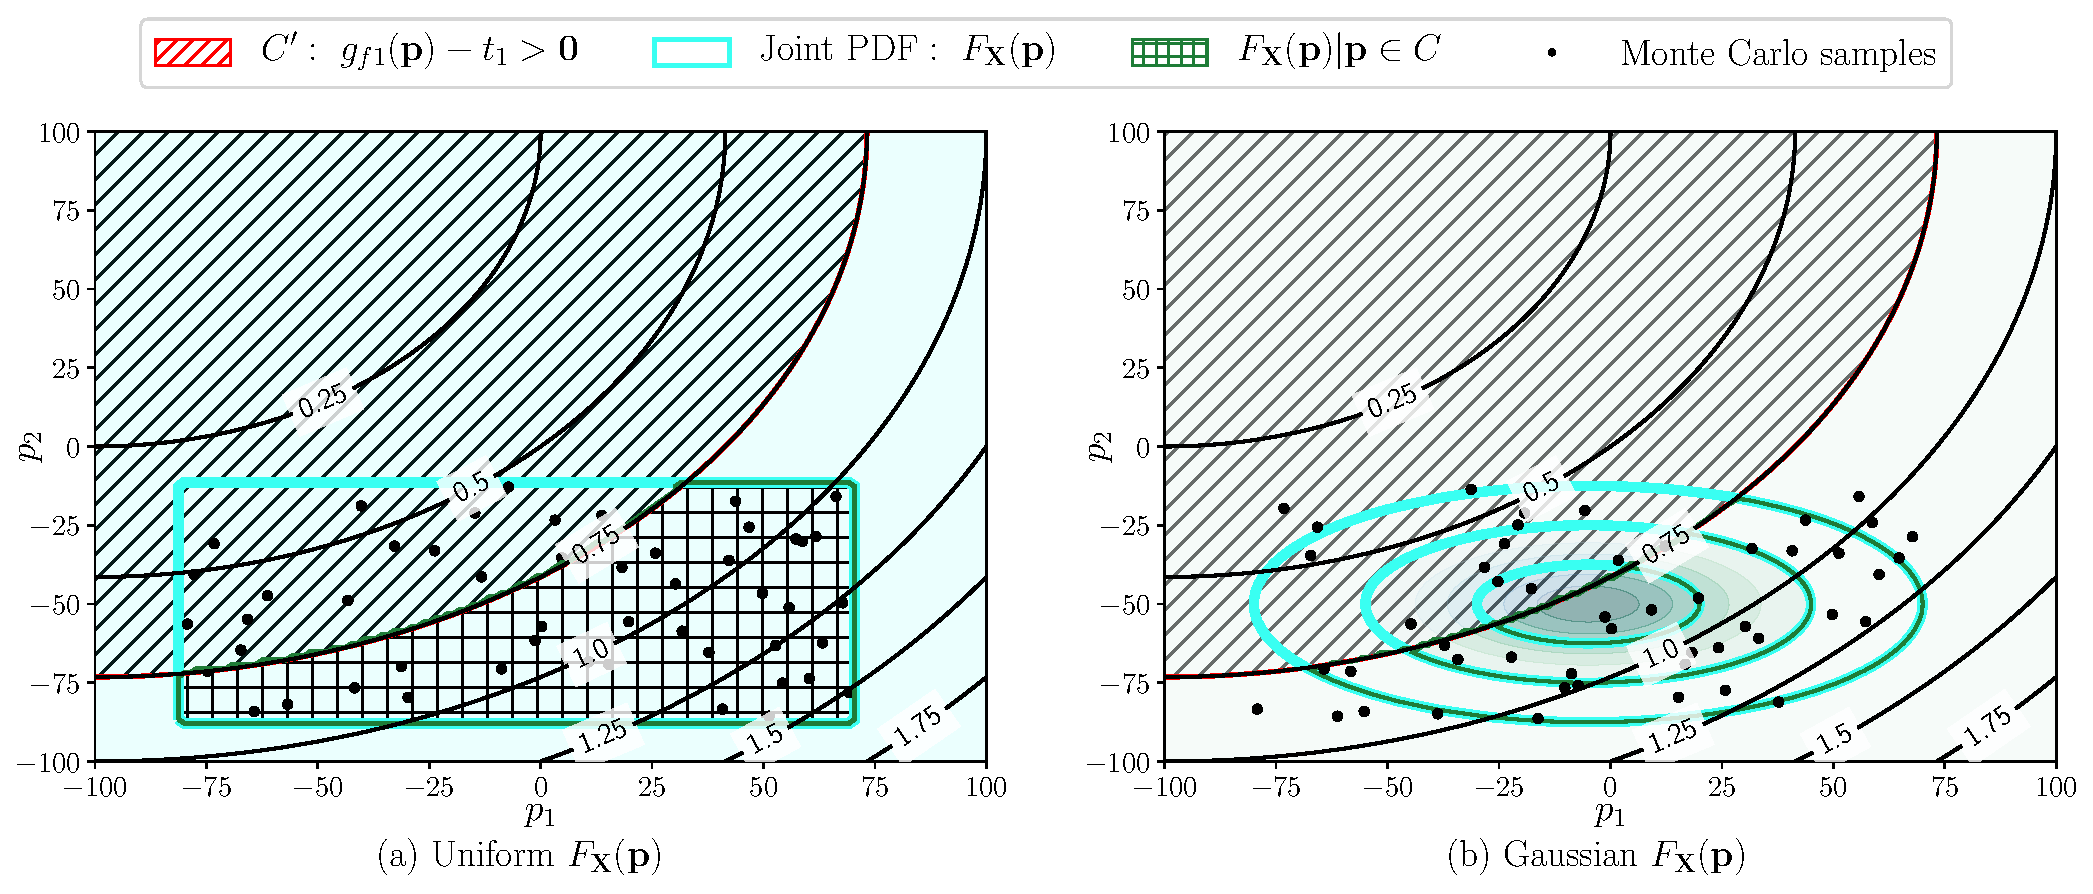
\includegraphics[width=0.9\textwidth]{1_2D_example_reliability.pdf}
	\caption{Contours of feasibility constraint $g_{f1}(\mathbf{p})$ in the 2 dimensional parameter space for different types of requirement \acp{PDF}}
	\label{fig:2Dexamplereliability}
\end{figure}

Only the Monte Carlo samples that lie within the set $C$ (shown as the unhatched region in Figure~\ref{fig:2Dexamplereliability}) are evaluated by $F_{\mathbf{X}}(\mathbf{p})$ and summed to compute the numerator of Equation~(\ref{eq:reliabilitymontecarlo}). All the Monte Carlo samples shown in Figure~\ref{fig:2Dexamplereliability} are evaluated by $F_{\mathbf{X}}(\mathbf{p})$ and summed to compute the denominator of Equation~(\ref{eq:reliabilitymontecarlo}). The reliability for the given requirement and capability can then be calculated as the quotient of the two sums.

We can now define buffer in the parameter space. Buffer is defined as the portion of the capability of a design reserved for changes in requirements \cite{Eckert2019}. In other words, the buffer set is defined as a set in the parameter space where sets $C$ and $R$ intersect.

\begin{equation} \label{eq:buffer}
	\textit{B} = \left\{\mathbf{p} \in \mathbb{R}^n~|~\mathbf{p} \in \left(C\cap R\right) \right\}.
\end{equation}

Excess is defined as the portion of the parameter space reserved for possible future changes in the requirements \cite{Eckert2019}. This is reflected by the set of parameter values that lie within the capability set $C$ but not within the requirement set $R$. 

\begin{equation} \label{eq:excess}
	\textit{E} = \left\{\mathbf{p} \in \mathbb{R}^n~|~\mathbf{p} \in \left(C\cap R'\right) \right\}.
\end{equation}

In other words, $B\cup E = C$.

The sets defined thus far are shown on the same 2-dimensional parameter space used for demonstrating the reliability calculation.

\begin{figure}[h!]
	\centering
	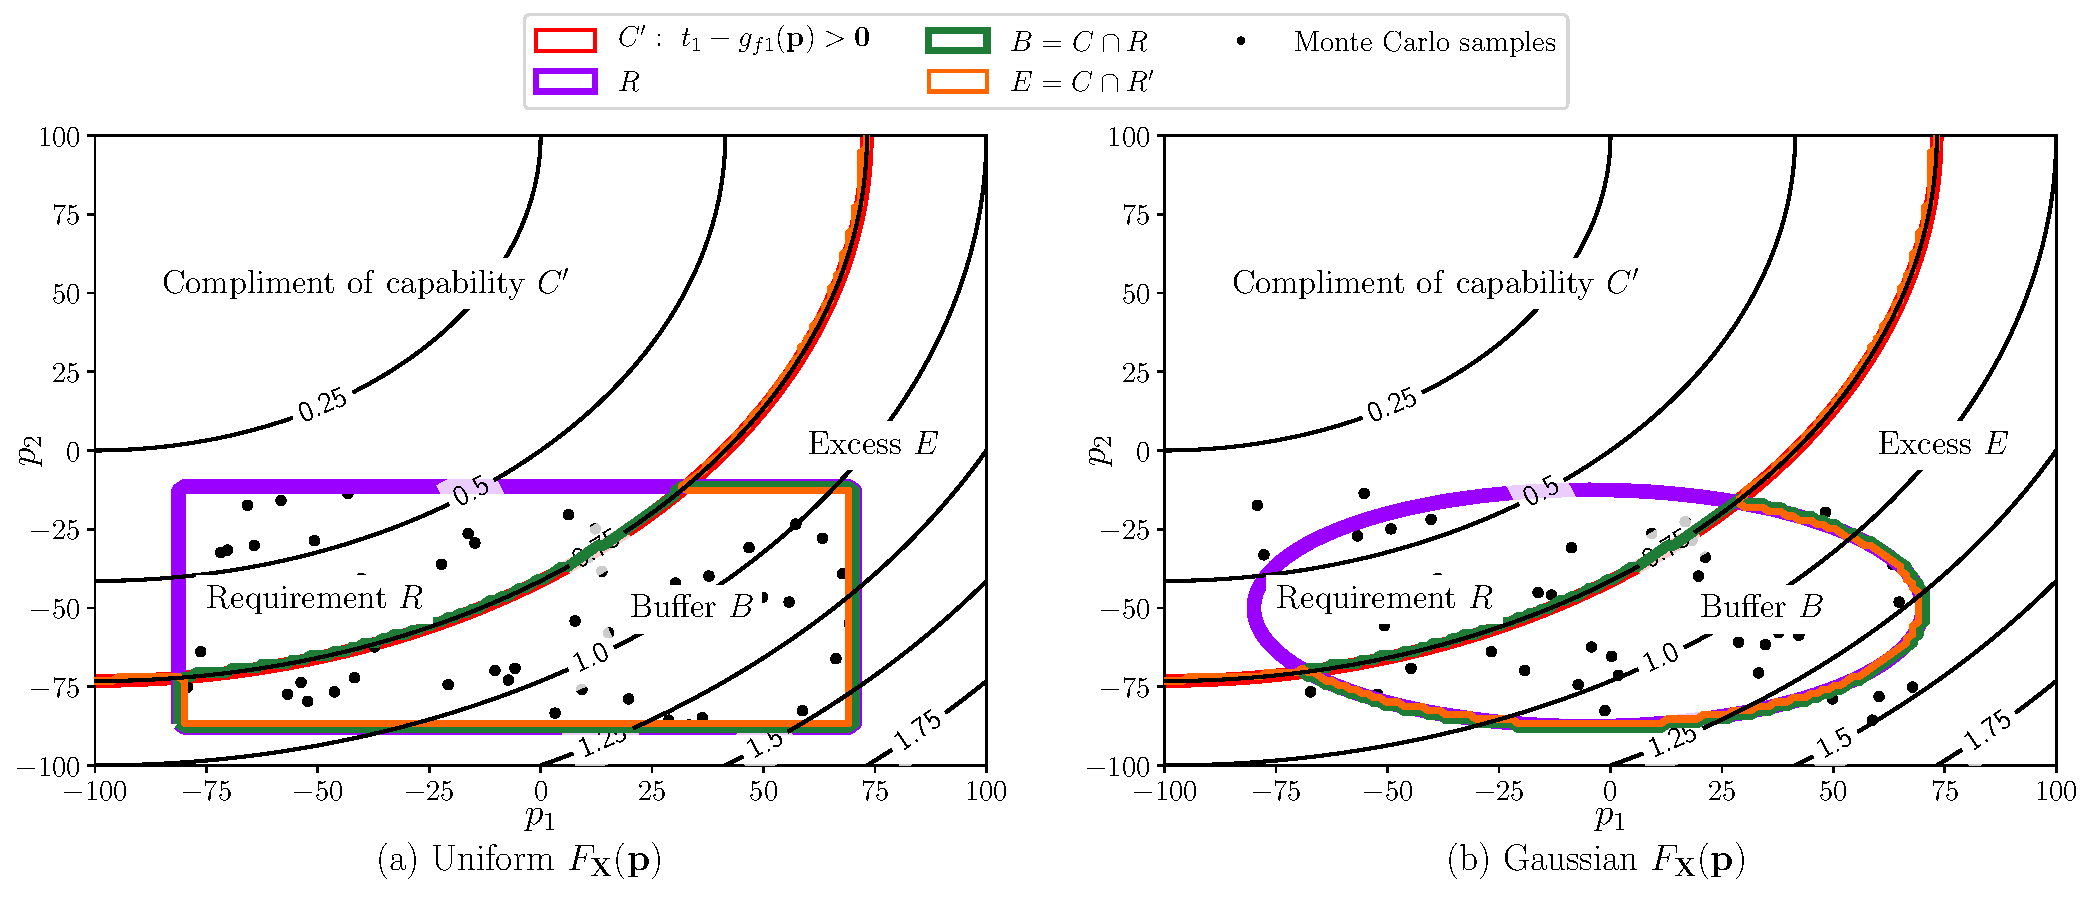
\includegraphics[width=0.9\textwidth]{2_2D_example_excess.pdf}
	\caption{Contours of feasibility constraint $g_{f1}(\mathbf{p})$ in the 2 dimensional parameter space for different types of requirement \acp{PDF}}
	\label{fig:2Dexampleexcess}
\end{figure}

We are particularly interested in minimizing excess during the product redesign cycle. We quantify excess using the volume of the set $E$. which can be found by Monte Carlo integration:

\begin{equation} \label{eq:excessmontecarlo}
	V_E \approx \dfrac{\sum\limits_{i=1}^{|{E}|} H\left(\mathbf{p}_i\right)}{\sum\limits_{i=1}^{N} H\left(\mathbf{p}_i\right)}, ~\mathrm{where}~ H\left(\mathbf{p}_i\right)={\begin{cases}1&{\text{if }}\mathbf{p}_i\in E\\0&{\text{else}}\end{cases}},
\end{equation}

and $N$ is the number of samples from the parameter space used for the integration such that $\mathbf{p}_i \in \mathbb{R}^n$. However, a large number of Monte Carlo samples is needed to capture the complex profile of the set $E$ in multi-dimensional parameter spaces.

We can make use of the reliability $\mathbb{P}(\mathbf{p} \in C)$ calculation and the volume of the requirement set $R$ to indirectly estimate the volume of set $E$. The volume of $R$ can be computed analytically for a uniform or Gaussian distribution as follows:

\begin{equation} \label{eq:Rmontecarlo}
	V_R = {\begin{cases} \prod\limits_{j=1}^{n} \left|b_j - a_j\right| &{\text{if }}F_\mathbf{X}(\mathbf{p})\text{ is uniform}\\\dfrac{\pi^2}{32}\prod\limits_{j=1}^{n} \left|b_j - a_j\right| &{\text{if }}F_\mathbf{X}(\mathbf{p})\text{ is Gaussian}\end{cases}},
\end{equation}

We can compute the volume of set $C$ using the following approach:

\begin{equation} \label{eq:Cmontecarlo}
	V_C \approx \dfrac{\sum\limits_{i=1}^{|{C}|} H\left(\mathbf{p}_i\right)}{\sum\limits_{i=1}^{N} H\left(\mathbf{p}_i\right)}, ~\mathrm{where}~ H\left(\mathbf{p}_i\right)={\begin{cases}1&{\text{if }}\mathbf{p}_i\in C\\0&{\text{else}}\end{cases}},
\end{equation}

The reliability approximates the percentage of $R$ in $C$ and can be used as as proxy for the volume of $C\cap R$ such that $V_{C\cap R} \approx \mathbb{P}(\mathbf{p} \in C) \times V_R$. $V_E$ can now be approximated using the following:

\begin{equation} \label{eq:excesssimple}
	V_E \approx V_C - \mathbb{P}(\mathbf{p} \in C) \times V_R,
\end{equation}

Having defined all the required design metrics, an optimization problem in terms of these metrics can be formulated such that excess is minimized while reliability constraints are met. We first define the context for the optimization problem in the form of an epoch-era analysis to simulate changing requirements throughout the product cycle.

%---------------------------------------------------------------------%
% Epoch era analysis
\subsection{Epoch era analysis for product redesign} \label{subsec:epochera}

We consider a problem where a product is redesigned as time progresses and the product advances through its development cycle or lifecycle. At every epoch in the product cycle, the designer must choose a redesign choice from a list of available options. This list of options is given by the set of redesign choices defined as the set of non-negative integers $\mathcal{D} = \left\{0,1,2,\cdots,q\right\}$. Chaining multiple choices together results in a design arc defined as:

\begin{equation} \label{eq:designarc}
	\mathbf{D} = \left[D_1 ~ D_2 ~ \cdots ~ D_o\right]^{\mathrm{T}},
\end{equation}

with possible choices $D_d \in \mathcal{D}^o$, where $1 \leq o \leq q+1$. The maximum number of redesign choices $q + 1$ dictates the maximum number of possible design arc combinations where no choice is repeated twice. For example, consider a case where there are $q + 1 = 3$ redesign choices. We drop the transpose operator $^{\mathrm{T}}$ when reporting design arcs in this thesis for convenience. The possible design arcs that can be obtained for the set of redesign choices $\mathcal{D} = \left\{0,1,2\right\}$ is:

\begin{equation*}
	\begin{aligned}
		& \mathbf{D}_1 = \left[0\right]\\
		& \mathbf{D}_2 = \left[0 ~ 1\right]\\
		& \mathbf{D}_3 = \left[0 ~ 1 ~ 2\right]\\
		& \mathbf{D}_4 = \left[0 ~ 2\right]\\
		& \mathbf{D}_4 = \left[0 ~ 2 ~ 1\right]\\
		& \mathbf{D}_4 = \left[1\right]\\
		& \mathbf{D}_4 = \left[1 ~ 0\right]\\
		& \mathbf{D}_4 = \left[1 ~ 0 ~ 2\right]\\
		& \mathbf{D}_4 = \left[1 ~ 2\right]\\
		& \mathbf{D}_4 = \left[1 ~ 2 ~ 0\right]\\
		& \mathbf{D}_4 = \left[2\right]\\
		& \mathbf{D}_4 = \left[2 ~ 0\right]\\
		& \mathbf{D}_4 = \left[2 ~ 0 ~ 1\right]\\
		& \mathbf{D}_4 = \left[2 ~ 1\right]\\
		& \mathbf{D}_4 = \left[2 ~ 1 ~ 0\right].\\
	\end{aligned}
\end{equation*}

These enumerations of the set $\mathcal{D}$ comprise a set of possible design arcs given by $\Omega_D$. The cardinality of $\Omega_D$ for a different number of redesign choices $q+1$ is given in Table~\ref{table:omegadcardinality}. The notation $|\Omega_D|$ is the cardinality operator applied to set $\Omega_D$.

\begin{table}[h!]
	\centering
	\renewcommand{\arraystretch}{1.0}% Wider
	\footnotesize\addtolength{\tabcolsep}{-5pt}
	\caption{Cardinality of set of possible design arcs $\mathbf{D}$}
	\label{table:omegadcardinality}
	\begin{tabular}{>{\centering\arraybackslash}p{2cm}>{\centering\arraybackslash}p{2cm}}
	\hline\hline
	\bf Number of redesign choices    & \bf Cardinality \\
	$q+1$ & $|\Omega_D|$ \\ \hline
	1  & 1 \\ 
	2 & 4 \\
	3 & 15 \\
	4 & 64 \\
	5 & 325 \\
	6 & 1956 \\
	\hline\hline
	\end{tabular}
\end{table}

We define a product cycle with $m$ number of epochs and $m$ number of corresponding decisions $S \in \mathcal{S}^m$, where $S_k$ is the decision at epoch $k$ and $\mathcal{S}$ is the set of possible decisions. In this chapter, we consider discrete redesign choices only. A non-negative integer value from the set $\mathcal{D}$ implies a redesign choice. A value of $-1$ implies no redesign is performed at the current epoch. This means that $\mathcal{S} = \left\{-1,0,1,2,\cdots,q\right\}$, where $q + 1$ is the number of available redesign choices.

The vector of all the decisions taken throughout the product cycle is referred to as the decision arc and is defined as follows:

\begin{equation} \label{eq:decisionarc}
	\mathbf{S} = \left[S_1 ~ S_2 ~ \cdots ~ S_m\right]^{\mathrm{T}}.
\end{equation}

We also drop the transpose operator $^{\mathrm{T}}$ when reporting decision arcs in this thesis for convenience. The set of possible decision arcs that can be generated from the set of possible decisions $\mathcal{S}$ is governed by some feasibility constraints. A feasible decision arc cannot contain repeated choices in a manner similar to design arcs $\mathbf{D}$. For example, the decision arc $\mathbf{S} = \left[0 ~ -1 ~ 0 ~ -1 ~ 1 ~ 3\right]$ is infeasible since the choice $0$ was repeated twice, while the decision arc $\mathbf{S} = \left[0 ~ -1 ~ 2 ~ -1 ~ 1 ~ 3\right]$ is feasible since it has no repeated choices. Furthermore, the first decision cannot be empty, i.e. $S_1 \neq -1$. This is because a decision arc must begin with some sort of design. These restrictions make computing the cardinality of the set of possible decision arcs $\Omega_S$ challenging. However, the cardinality of $\Omega_S$ is given by a finite positive integer similar to $\Omega_D$ in Table~\ref{table:omegadcardinality}.

A corresponding design arc can be extracted from the decision arc by removing all negative elements from $\mathbf{S}$ to obtain $\mathbf{D} = \left[0 ~ 2 ~ 1 ~ 3\right]$. 

For each epoch $k$, a design arc can be extracted by excluding values from $\mathbf{S}$ that are equal to $-1$. The vector $\mathbf{D}_k = \left[D_1 ~ D_2 ~ \cdots ~ D_o\right]$ represents this design arc at epoch $k$ where the elements of $\mathbf{D}$ are non-negative integers and $o$ is the number of non-negative integers in $\left[S_1 ~ S_2 ~ \cdots ~ S_k\right]$ up to the current epoch $k$. For example, consider the following decision arc for a problem with $m=6$ epochs:

\begin{equation*} \label{eq:decisionarcex}
	\mathbf{S} = \left[0 ~ -1 ~ 2 ~ -1 ~ 1 ~ 3\right].
\end{equation*}

$m$ design arcs can be extracted from $\mathbf{S}$ at each epoch.

\begin{equation*}
	\begin{aligned}
		& \mathrm{epoch~} k=1: \mathbf{D}_1 = \left[0\right]\\
		& \mathrm{epoch~} k=2: \mathbf{D}_2 = \left[0\right]\\
		& \mathrm{epoch~} k=3: \mathbf{D}_3 = \left[0 ~ 2\right]\\
		& \mathrm{epoch~} k=4: \mathbf{D}_4 = \left[0 ~ 2\right]\\
		& \mathrm{epoch~} k=5: \mathbf{D}_5 = \left[0 ~ 2 ~ 1\right]\\
		& \mathrm{epoch~} k=6: \mathbf{D}_6 = \left[0 ~ 2 ~ 1 ~ 3\right].\\
	\end{aligned}
\end{equation*}

Logically, it follows that each design arc cannot feature repeated elements due to the uniqueness of the positive decision arc elements. Each design arc has a unique capability set $C_k$.

We now define the requirement arc as a vector of joint \acp{PDF} that has $m$ elements. Each element corresponds to a different epoch $k$ with a requirement joint \ac{PDF} $F_{\mathbf{X}k}(\mathbf{p})$. The requirement arc is defined as follows:

\begin{equation} \label{eq:requirementarc}
	\mathbf{R} = \left[F_{\mathbf{X}1}(\mathbf{p}) ~ F_{\mathbf{X}2}(\mathbf{p}) ~ \cdots ~ F_{\mathbf{X}m}(\mathbf{p})\right]^{\mathrm{T}}.
\end{equation}

The reliability at epoch $k$, $\mathbb{P}_k(\mathbf{p} \in C_k)$ can be calculated from $C_k$ (derived from $\mathbf{D}_k$) and the requirement joint \ac{PDF} $F_{\mathbf{X}k}(\mathbf{p})$ to yield a reliability vector defined as follows:

\begin{equation} \label{eq:reliabilityvector}
	\mathbf{P}(\mathbf{p} \in \mathbf{C}) = \left[\mathbb{P}_1(\mathbf{p} \in C_1) ~ \mathbb{P}_2(\mathbf{p} \in C_2) ~ \cdots ~ \mathbb{P}_m(\mathbf{p} \in C_m)\right]^{\mathrm{T}},
\end{equation}

where $\mathbf{C}$ is the vector of capability sets $\mathbf{C} = \left[C_1 ~ C_2 ~ \cdots ~ C_m\right]^{\mathrm{T}}$.

At each epoch, a reliability threshold $P_k$ is defined to yield a vector of reliability thresholds defined as follows:

\begin{equation} \label{eq:reliabilitythvector}
	\mathbf{P}_{th} = \left[P_1 ~ P_2 ~ \cdots ~ P_m\right]^{\mathrm{T}}.
\end{equation}

The volume of the excess set at epoch $k$, $V_{Ek}$ can be calculated from $C_k$ and the requirement joint \ac{PDF} $F_{\mathbf{X}k}(\mathbf{p})$ using Equations~(\ref{eq:excess}) and (\ref{eq:excesssimple}) to yield an excess vector defined as follows:

\begin{equation} \label{eq:excessvector}
	\mathbf{E} = \left[V_{E1} ~ V_{E2} ~ \cdots ~ V_{Em}\right]^{\mathrm{T}},
\end{equation}

The cumulative excess for a given decision arc can be formulated as:

\begin{equation} \label{eq:excesscumulative}
	E_c = \sum\limits_{k=1}^{m} V_{Ek}.
\end{equation}

In addition to the decision arc $\mathbf{S}$, a fixed design concept $c_t\in\mathcal{C}$ is defined. The concept type $c_t$ is selected at the very beginning of the epoch-era analysis and does not change throughout epochs. The choice of $c_t$ dictates the list of redesign choices available for the remainder of the product cycle. $\mathcal{C}$ is the set of concept choices whose elements are all non-negative integers. This means that $\mathcal{C} = \left\{0,1,2,\cdots,r\right\}$, where $r + 1$ is the number of available concept choices.

Each concept type $C_t$ has a set of redesign options $\mathcal{D}_t$ with $q+1$ redesign choices attached to it. Accordingly, each concept type $c_t$ will have a set of possible design arcs $\Omega_{Dt}$ and a set of possible decision arcs $\Omega_{St}$. The combination of a concept and design arc $\left\{c,\mathbf{D}\right\}$ will be referred to as a design arc in this thesis for conciseness. Similarly, the combination of a concept and a decision arc $\left\{c,\mathbf{S}\right\}$ will be referred to as a decision arc.

The cardinality of the set of possible design arcs $\Omega_{cD}$ is simply obtained by adding the cardinalities of all the sets $\Omega_{Dt}$ for a given set of concept choices $\mathcal{C}$:

\begin{equation} \label{eq:cardinailitycdarc}
	\beta = |\Omega_{cD}| = \sum\limits_{t=0}^{r} |\Omega_{Dt}|,
\end{equation}

where $|\Omega_{Dt}|$ can be obtained from Table~\ref{table:omegadcardinality} knowing the number of redesign choices $q+1$ for each concept. The set of possible design arcs represents the feasible design space in this chapter and is defined as follows:

\begin{equation} \label{eq:feasibledesignset}
	\Omega_{cD} = \left\{\left\{c,\mathbf{D}\right\}_1,\left\{c,\mathbf{D}\right\}_2,\cdots,\left\{c,\mathbf{D}\right\}_\beta\right\}.
\end{equation}

A similar approach can be used to calculate the cardinality of the set of possible decision arcs $\Omega_{cS}$ although we do not need to compute it in this chapter.

\begin{equation} \label{eq:cardinailitycsarc}
	|\Omega_{cS}| = \sum\limits_{t=0}^{r} |\Omega_{St}|.
\end{equation}

We now formulate an optimization problem for choosing the optimal concept $c$ and decision arc $\mathbf{S}$ such that cumulative excess $E_c$ is minimized subject to reliability constraints $\mathbf{g}(c,\mathbf{S}) = \mathbf{P}_{th} - \mathbf{P}(\mathbf{p} \in \mathbf{C}) \le \mathbf{0}$:

\begin{equation}
	\label{eq:TSEoptproblem}
	\begin{aligned}
		& \underset{\{c,\mathbf{S}\}\in\Omega_{cS}}{\text{minimize}}
		& & {f}(c,\mathbf{S};\mathbf{R}) = E_c = \sum\limits_{k=1}^{m} V_{Ek}(c,\mathbf{D}_k;F_{\mathbf{X}k}(\mathbf{p}))\\
		& \text{subject to}
		& & \mathbf{g}(c,\mathbf{S};\mathbf{R}) = \mathbf{P}_{th} - \mathbf{P}(\mathbf{T} \in \mathbf{C}) \le \mathbf{0}\\
		& \text{where,}
		& & \Omega_{cS}\text{: all feasible decision arcs}.\\
	\end{aligned}
\end{equation}

We also define a second optimization problem to simulate the effect of accumulating costs that can be incurred throughout a product's lifecycle. Since we focus on aerospace applications in this chapter, we consider the cumulative weight of the decision arc to be a reflection of cumulative costs such as fuel.

\begin{equation}
	\label{eq:optproblemweight}
	\begin{aligned}
		& \underset{\{c,\mathbf{S}\}\in\Omega_{cS}}{\text{minimize}}
		& & {f}(c,\mathbf{S}) = W_c = \sum\limits_{k=1}^{m} W_{k}(c,\mathbf{D}_k)\\
		& \text{subject to}
		& & \mathbf{g}(c,\mathbf{S};\mathbf{R}) = \mathbf{P}_{th} - \mathbf{P}(\mathbf{T} \in \mathbf{C}) \le \mathbf{0}\\
		& \text{where,}
		& & \Omega\text{: all feasible decision arcs}.\\
	\end{aligned}
\end{equation}

The problem in Equation~(\ref{eq:TSEoptproblem}) is solved using a combinatorial optimization algorithm rather than a discrete optimization algorithm. This is because the feasible set $\Omega_{cS}$ is not given by the possible combinations of integers in $\mathcal{S} = \left\{-1,0,1,2,\cdot,q\right\}$. The choice of concept is restricted to non-negative integers, while the decision arc may not feature repeated non-negative integers as explained earlier. As a result, the set $\Omega_{cS}$ must be algorithmically defined as is done with combinatorial optimization problems.

The optimization problems given by Equations~(\ref{eq:TSEoptproblem}) and Equations~(\ref{eq:optproblemweight}) yield a solution $\mathbf{x}^*(\mathbf{R})$ which depends on the requirement arc. The nature of requirements is that they are subject to change. As a result, we adopt a set-based design strategy to manage changing requirements.

%---------------------------------------------------------------------%
% Set-based approach
\subsection{Set-based design for uncertain requirements} \label{subsec:SBDproblem}

%f: objective functions
%g: constraint functions
%n: dimensionality of parameter space
%i: requirement set sample index 
%j: element index of bound vectors for Gaussian and uniform pdfs
%m: number of stages
%k: index of stage
%o: number of designs in design arcs
%d: index of design decision in design arc
%q: number of redesign (deposit) choices
%r: number of concept choices
%s: number of SBD requirement arc samples (cardinality)
%w: index of requirement arc sample
%v: number of choices for joint PDF
%t: type of PDF set
%e: number of linear interpolation samples for generating R_v
%\alpha: number of designs for cut-off
%\beta: number of possible concept/design arcs
%\lambda: index of concept/design arcs
%\zeta: number of possible enumerations of decision arcs from design arcs
%\gamma: index of decision arc in enumerations from design arcs

The set-based design strategy involves sampling requirement arcs $\mathbf{R}$ from the set of possible requirement arcs $\Omega_R$. A sample from the set $\Omega_R$, $\mathbf{R}_w$ involves populating the requirement arc with joint \acp{PDF} at each epoch $k$ by selecting a joint \ac{PDF} from the set of possible joint \acp{PDF} $\mathcal{R} = \left\{F_{\mathbf{X}1}(\mathbf{p}),F_{\mathbf{X}2}(\mathbf{p}),\cdots,F_{\mathbf{X}v}(\mathbf{p})\right\}$, where $v$ is the number of joint \ac{PDF} choices. $\mathbf{R}_w$ is constructed by selecting $m$ joint \acp{PDF} from $\mathcal{R}$ such that $\mathbf{R}_w \in \mathcal{R}^m$. $\Omega_R$ is now defined as:

\begin{equation} \label{eq:Rarcsample}
	\Omega_R = \left\{\mathbf{R}_1,\mathbf{R}_2\cdots,\mathbf{R}_s\right\},
\end{equation}

where $s = |\Omega_R|$ is the cardinality of $\Omega_R$.

The set of joint \ac{PDF} choices $\mathcal{R}$ is constructed by generating different joint \acp{PDF} defined by their mean vector $\boldsymbol{\mu}$, interval $\boldsymbol{\sigma}$ and type $t\in\mathcal{T} = \left\{\mathrm{``Uniform"},\mathrm{``Gaussian"}\right\}$. The interval $\boldsymbol{\sigma}$ is the same as the standard deviation vector defined for the Gaussian joint \ac{PDF} in Equation~(\ref{eq:gaussianpdf}). For a uniform joint \ac{PDF}, the bounds are obtained from the interval vector such that $\mathbf{a} = \boldsymbol{\mu} - 3\boldsymbol{\sigma}$ and $\mathbf{b} = \boldsymbol{\mu} + 3\boldsymbol{\sigma}$. This allows any joint \ac{PDF} to be fully parametrized by three parameters, the type $t$, the mean vector $\boldsymbol{\mu}$ and the interval vector $\boldsymbol{\sigma}$.

The method for populating the set $\mathcal{R}$ is based on the designer's experience with the requirements and previous knowledge. For example if requirements are expected to become well-defined over time around a certain value in the parameter space, then a set of mean vectors $M = \left\{\boldsymbol{\mu}_1,\boldsymbol{\mu}_2,\cdots,\boldsymbol{\mu}_e\right\}$ and a set of interval vectors $\Sigma = \left\{\boldsymbol{\sigma}_1,\boldsymbol{\sigma}_2,\cdots,\boldsymbol{\sigma}_e\right\}$ can be obtained by linearly interpolating between the start and end states given by $\boldsymbol{\mu}_1,\boldsymbol{\sigma}_1$ and $\boldsymbol{\mu}_e,\boldsymbol{\sigma}_e$ respectively for each type of joint \ac{PDF}. 

An example of this kind of interpolation search strategy is shown in Figure~\ref{fig:2Dexampleinterp} for the same 2D example used in Section~\ref{subsec:designmetrics}.

\begin{figure}[h!]
	\centering
	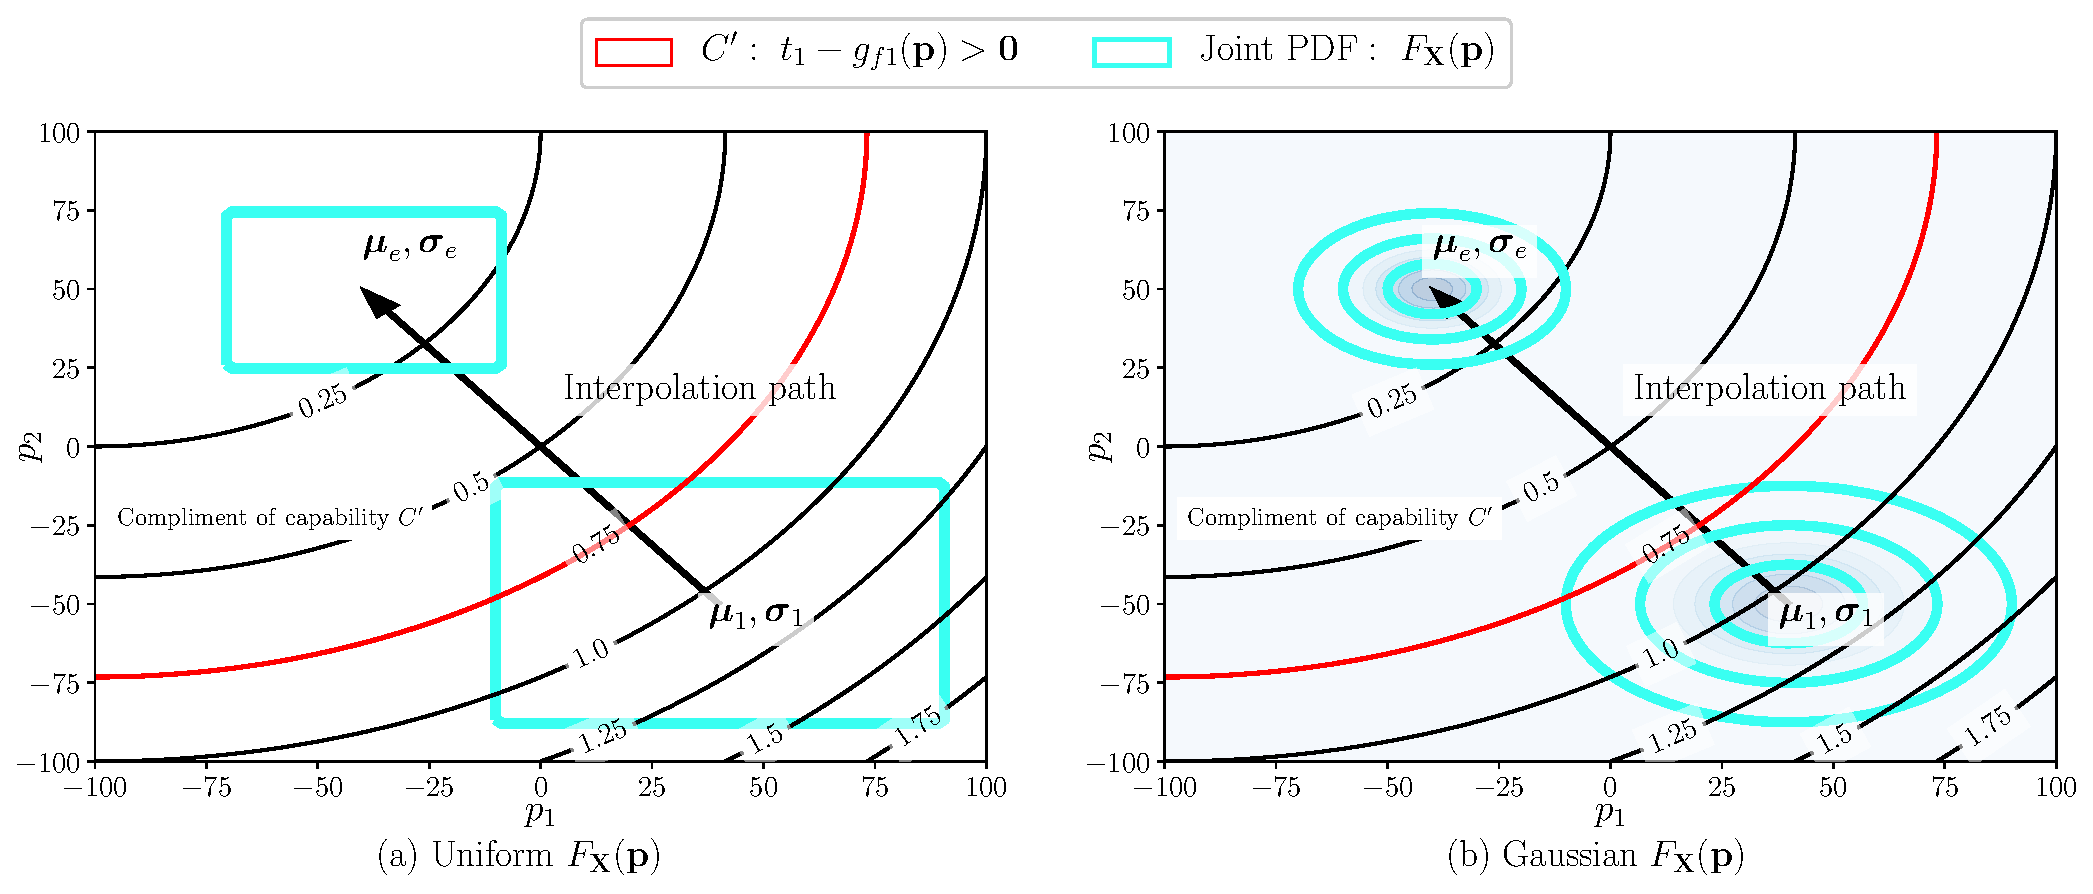
\includegraphics[width=0.9\textwidth]{3_2D_example_interpolation.pdf}
	\caption{Contours of feasibility constraint $g_{f1}(\mathbf{p})$ in the 2 dimensional parameter space for different types of requirement \acp{PDF}}
	\label{fig:2Dexampleinterp}
\end{figure}

The set of possible requirement arcs $\Omega_R$ spans every possible combination of the joint \ac{PDF} types $t$, means $M$ and intervals $\Sigma$. Consider an example with $m=6$ epochs. If $e=5$ interpolation levels are used to obtain $M$ and $\boldsymbol{\Sigma}$ and two \ac{PDF} types $\mathcal{T} = \left\{\mathrm{``Uniform"},\mathrm{``Gaussian"}\right\}$ are available, the number of choices $v$ for $\mathcal{R}$ and the cardinality $s$ for $\Omega_R$ is calculated as follows:

\begin{equation*}
	\begin{aligned}
		& v = e \times e \times |\mathcal{T}| = 5 \times 5 \times 2 = 50,\\
		& s = |\Omega_R| = m^v = 6^{50},~\mathrm{respectively}.\\
	\end{aligned}
\end{equation*}

It can be deduced that a small increase in the number of joint \ac{PDF} choices causes the cardinality of $\Omega_R$ to increase exponentially. For practicality only the first few elements of $\Omega_R$ will be used during the set-based design analysis and $s$ will be capped at $10^5$ samples. The reasons for this choice will be explained in results section~\ref{sec:TSEresults}.

The first set-based solution is obtained by solving the optimization problem in Equation~(\ref{eq:TSEoptproblem}) for every requirement arc sample $\mathbf{R}_w$ in $\Omega_R$ to obtain a corresponding solution $\mathbf{x}_S^*(\mathbf{R}_w) = \left\{c^*,\mathbf{S}^*\right\}(\mathbf{R}_w)$. In order to compare the overdesign levels across different design arcs rather than different decision arcs, the corresponding optimal design arc $\mathbf{D}^*$ can be extracted from the optimal decision arc $\mathbf{S}^*$ to obtain the solution $\mathbf{x}^*(\mathbf{R}_w) = \left\{c^*,\mathbf{D}^*\right\}(\mathbf{R}_w)$

The set of parametric optimal design arcs with respect to excess is defined as:

\begin{equation} \label{eq:SBDexcessopt}
	S_E^* = \left\{\mathbf{x}^*(\mathbf{R}_1),\mathbf{x}^*(\mathbf{R}_2)\cdots,\mathbf{x}^*(\mathbf{R}_s)\right\}.
\end{equation}

We track the number of times a specific design arc $\left\{c,\mathbf{D}\right\}_\lambda$ appears as the solution to the parametric optimization problem in $S_E^*$ via a design optimality vector defined as follows:

\begin{equation} \label{eq:robustnessvec}
	\mathbf{N}_E = \left[n_{E1} ~ n_{E2} ~ \cdots ~ n_{E\beta}\right]^{\mathrm{T}},
\end{equation}

where $n_{E\lambda}$ is equal to the number of times design arc $\left\{c,\mathbf{D}\right\}_\lambda \in \Omega_{cD}$ is repeated in $S_E^*$ and gives the frequency of each design arc. The top $\alpha$ design arcs with the largest $n_{E\lambda}$ values are selected as the set-based solution representing the best performing design arcs in terms of minimizing over-design.

\begin{equation} \label{eq:SBDexcess}
	S_E = \left\{\left\{c,\mathbf{D}\right\}_{E1},\left\{c,\mathbf{D}\right\}_{E2}\cdots,\left\{c,\mathbf{D}\right\}_{E\alpha}\right\},
\end{equation}

where the subscript $E1,E2,\cdots,E\alpha$ indicates that the corresponding base is ordered by frequency in the set of parametric optimal solutions with respect to excess $S_E^*$.

The same procedure is repeated for the optimization problem in Equation~(\ref{eq:optproblemweight}) to obtain the second set-based solution comprising the best performing design arcs in terms of minimizing weight throughout the product cycle:

\begin{equation} \label{eq:SBDexcess}
	S_W = \left\{\left\{c,\mathbf{D}\right\}_{W1},\left\{c,\mathbf{D}\right\}_{W2}\cdots,\left\{c,\mathbf{D}\right\}_{W\alpha}\right\},
\end{equation}

where the subscripts $W1,W2,\cdots,W\beta$ indicate that the corresponding base is ordered by frequency in the set of parametric optimal solutions with respect to weight $S_W^*$.

Algorithm~\ref{algo:SBDOptalgo} describes the methodology to be followed for obtaining the sets of optimal design arcs with respect to excess or weight.

\begin{algorithm}
	\DontPrintSemicolon % Some LaTeX compilers require you to use \dontprintsemicolon instead
	\KwIn{
		Set of possible requirement arcs $\Omega_R$, Set of possible design arcs $\Omega_{cD}$
	}
	\KwOut{$S_{E}$}
	Initialize design optimality vector $\mathbf{N}_E = \left[n_{E1},n_{E2},\cdots,n_{E\beta}\right] = \mathbf{0}$\;	
	\For{$w \gets 1$ to $s$} {
		Solve the parametric optimization problem in Equation~(\ref{eq:TSEoptproblem}) to obtain optimal decision arc $\mathbf{x}_S^*(\mathbf{R}_w) = \left\{c^*,\mathbf{S}^*\right\}(\mathbf{R}_w)$\;
		Reduce optimal decision arc to optimal design arc by eliminating $-1$ components of $\mathbf{S}^*$ to obtain $\mathbf{x}^*(\mathbf{R}_w) = \left\{c^*,\mathbf{D}^*\right\}(\mathbf{R}_w)$\;
		Augment $S_{E}^* \gets S_{E}^* \cup \{ \mathbf{x}^*(\mathbf{R}_w) \} $\;
		Find $\lambda$ corresponding to $\left\{c^*,\mathbf{D}^*\right\}$\;
		Award design arc $n_{E\lambda} \gets n_{E\lambda} + 1$\;
	}
	Sort design optimality vector $\mathbf{N}_E$ in descending order\;
	Select top $\alpha$ design arcs with largest values $n_{E\lambda}$ to obtain set of optimal designs $S_E = \left\{\left\{c,\mathbf{D}\right\}_{E1},\left\{c,\mathbf{D}\right\}_{E2}\cdots,\left\{c,\mathbf{D}\right\}_{E\alpha}\right\}$\;
	\caption{Pseudo-algorithm for obtaining the set of optimal design arcs $S_{E}$}
	\label{algo:SBDOptalgo}
\end{algorithm}

The third set-based solution is the robust design set. We define robustness of a design arc by the number of design arcs satisfied from the set $\Omega_R$. We evaluate the feasibility of each design arc $\left\{c,\mathbf{D}\right\}_\lambda$ sampled from the set of possible design arcs in Equation~(\ref{eq:feasibledesignset}) with respect to every requirement arc $\mathbf{R}_w$ in $\Omega_R$.

We generate all the possible decision arcs for a given design arc $\left\{c,\mathbf{D}\right\}_\lambda$. These combinations are generated by randomly inserting the $-1$ decisions into the design arc vector until it has the same number of elements as the number of epochs $m$. We show this using an example. Consider the design arc $\left\{c = 1,\mathbf{D} = \left[2 ~ 0 ~ 1\right]\right\}$. The possible decision arcs are:

\begin{equation*}
	\begin{aligned}
		& \left\{c = 1,\mathbf{S} = \left[2 ~ -1 ~ -1 ~ -1 ~ 0 ~ 1\right]\right\}\\
		& \left\{c = 1,\mathbf{S} = \left[2 ~ -1 ~ -1 ~ 0 ~ -1 ~ 1\right]\right\}\\
		& \left\{c = 1,\mathbf{S} = \left[2 ~ -1 ~ -1 ~ 0 ~ 1 ~ -1\right]\right\}\\
		& \left\{c = 1,\mathbf{S} = \left[2 ~ -1 ~ 0 ~ -1 ~ 1 ~ -1\right]\right\}\\
		& \left\{c = 1,\mathbf{S} = \left[2 ~ -1 ~ 0 ~ 1 ~ -1 ~ -1\right]\right\}\\
		& \left\{c = 1,\mathbf{S} = \left[2 ~ 0 ~ -1 ~ 1 ~ -1 ~ -1\right]\right\}\\
		& \left\{c = 1,\mathbf{S} = \left[2 ~ 0 ~ 1 ~ -1 ~ -1 ~ -1\right]\right\}.\\
	\end{aligned}
\end{equation*}

These enumerations result in a set of the decision arcs defined as follows:

\begin{equation} \label{eq:enumeratedcS}
	S_{cD} = \left\{\left\{c,\mathbf{S}\right\}_{1},\left\{c,\mathbf{S}\right\}_{2}\cdots,\left\{c,\mathbf{S}\right\}_{\zeta}\right\},\mathrm{~where~} \left\{c,\mathbf{S}\right\}_{\gamma} \in S_{cD}
\end{equation}

and $\zeta$ is the number of possible enumerations. In the previous example $\zeta = 7$.

The feasibility in terms of reliability is checked for every possible decision arc $\left\{c,\mathbf{S}\right\}_{\gamma}$ for a given $\left\{c,\mathbf{D}\right\}_\lambda$ and requirement arc $\mathbf{R}_w$ using $\mathbf{g}(c_{\gamma},\mathbf{S}_{\gamma};\mathbf{R}_w) = \mathbf{P}_{th} - \mathbf{P}(\mathbf{T} \in \mathbf{C}) \le \mathbf{0}$. If any of the decision arcs in set $S_{cD}$ satisfy all the reliability constraints then the corresponding design arc $\left\{c,\mathbf{D}\right\}_\lambda$ is considered feasible. We track the number of requirement arcs satisfied by design arc $\left\{c,\mathbf{D}\right\}_\lambda$ through a robustness vector defined as follows:

\begin{equation} \label{eq:robustnessvec}
	\mathbf{N}_R = \left[n_{R1} ~ n_{R2} ~ \cdots ~ n_{R\beta}\right]^{\mathrm{T}},
\end{equation}

where $n_{R\lambda}$ is equal to the number of requirement arcs $\mathbf{R}_w \in \Omega_R$ satisfied by design arc $\left\{c,\mathbf{D}\right\}_\lambda \in \Omega_{cD}$. The top $\alpha$ design arcs with the largest $n_{R\lambda}$ values are considered as the robust design set.

\begin{equation} \label{eq:SBDrobust}
	S_R = \left\{\left\{c,\mathbf{D}\right\}_{R1},\left\{c,\mathbf{D}\right\}_{R2}\cdots,\left\{c,\mathbf{D}\right\}_{R\alpha}\right\},
\end{equation}

where the subscripts $R1,R2,\cdots,R\alpha$ indicate that these design arcs are ordered by number of requirement arcs satisfied from the set $\Omega_R$.

The final set-based solution is the flexible design set. All the possible design arcs form the set $\Omega_{cD}$ are ranked in terms of filtered outdegree. The filtered outdegree is defined as the number of possible design arcs that can be obtained from the current design arc by adding exactly one redesign choice that is not an element of the current design arc. The filtered outdegree for a design arc $\left\{c,\mathbf{D}\right\}_\lambda$ having $o$ elements and $q + 1$ redesign choices is simply equal to:

\begin{equation} \label{eq:filteredoutdegree}
	FO_{\lambda} = q - o.
\end{equation}

The top $\alpha$ design arcs in terms of filtered outdegree are considered as the flexible design set.

\begin{equation} \label{eq:SBDflexible}
	S_F = \left\{\left\{c,\mathbf{D}\right\}_{F1},\left\{c,\mathbf{D}\right\}_{F2}\cdots,\left\{c,\mathbf{D}\right\}_{F\alpha}\right\},
\end{equation}

where the subscript $F1,F2,\cdots,F\alpha$ indicate that these design arcs are ordered by filtered outdegree $FO$.

Algorithm~\ref{algo:SBDRobustalgo} describes the methodology to be followed for obtaining the sets of optimal design arcs with respect to excess or weight.

\begin{algorithm}
	\DontPrintSemicolon % Some LaTeX compilers require you to use \dontprintsemicolon instead
	\KwIn{
		Set of possible requirement arcs $\Omega_R$, Set of possible design arcs $\Omega_{cD}$
	}
	\KwOut{$S_{R}$, $S_{F}$}
	Initialize design robustness vector $\mathbf{N}_R = \left[n_{R1},n_{R2},\cdots,n_{R\beta}\right] = \mathbf{0}$\;	
	\For{$\lambda \gets 1$ to $\beta$} {
		Enumerate possible decision arcs from $\left\{c,\mathbf{D}\right\}_\lambda$ to obtain the set $S_{cD} = \left\{\left\{c,\mathbf{S}\right\}_{1},\left\{c,\mathbf{S}\right\}_{2}\cdots,\left\{c,\mathbf{S}\right\}_{\zeta}\right\}$\;
		\For{$w \gets 1$ to $s$} {
			\For{$\gamma \gets 1$ to $\zeta$} {
				
				\If{$\mathbf{g}(c,\mathbf{S};\mathbf{R}) \le \mathbf{0}$} {
					Award design arc $n_{R\lambda} \gets n_{R\lambda} + 1$\;
					\textbf{break}
				}
			
			}
		}
		Compute filtered outdegree for $\left\{c,\mathbf{D}\right\}_\lambda$ using $FO_{\lambda} = q - o$\;
		Augment design flexibility vector $\mathbf{N}_F \gets \mathbf{N}_F \cup \{ FO_{\lambda} \} $\;
	}
	Sort design robustness vector $\mathbf{N}_R$ in descending order\;
	Select top $\alpha$ design arcs with largest values $n_{R\lambda}$ to obtain set of robust design arcs $S_R = \left\{\left\{c,\mathbf{D}\right\}_{R1},\left\{c,\mathbf{D}\right\}_{R2}\cdots,\left\{c,\mathbf{D}\right\}_{R\alpha}\right\}$\;
	Sort design flexibility vector $\mathbf{N}_F$ in descending order\;
	Select top $\alpha$ design arcs with largest values $FO_{\lambda}$ to obtain set of flexible design arcs $S_F = \left\{\left\{c,\mathbf{D}\right\}_{F1},\left\{c,\mathbf{D}\right\}_{F2}\cdots,\left\{c,\mathbf{D}\right\}_{F\alpha}\right\}$\;
	\caption{Pseudo-algorithm for obtaining the sets of robust and flexible design arcs $S_{E}^*$}
	\label{algo:SBDRobustalgo}
\end{algorithm}

We summarize the procedure for obtaining the set-based solutions $S_E,S_W,S_R$ and $S_F$ in Figure~\ref{fig:methodology}.

\begin{figure}[h!]
	\centering
	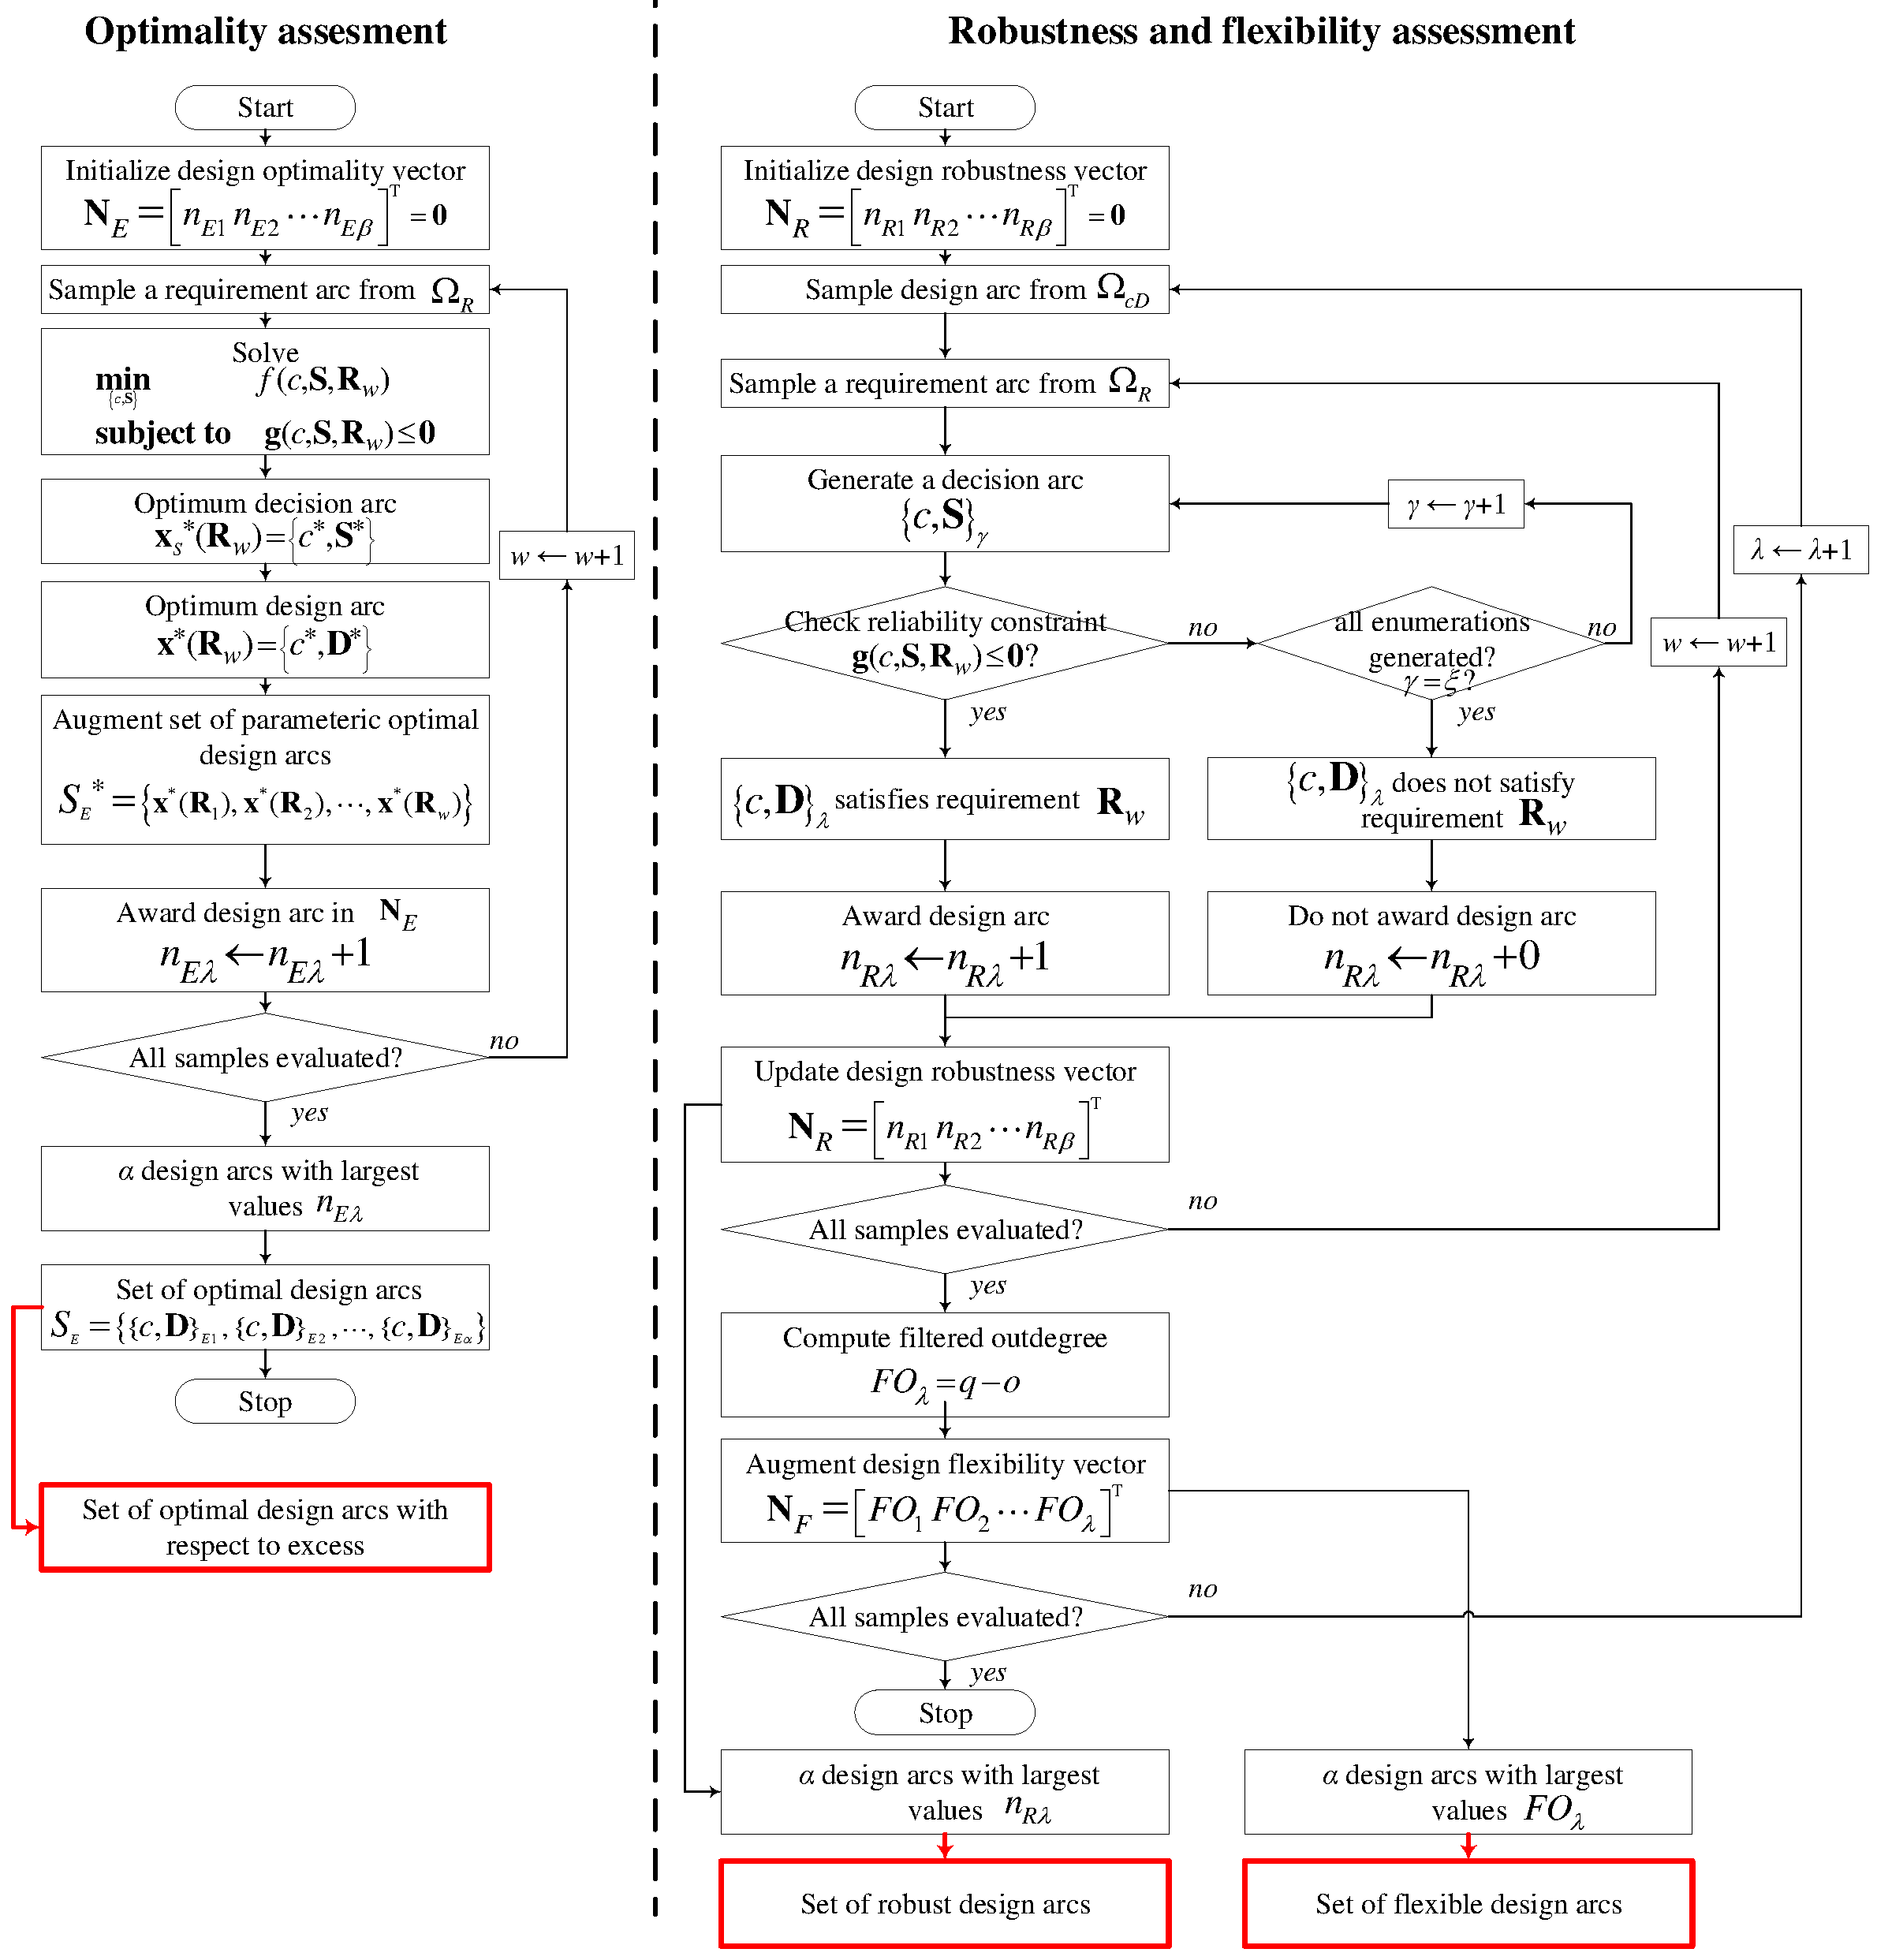
\includegraphics[width=0.99\textwidth]{4_methodology_V2.pdf}
	\caption{Summary of methodology for generating set-based solutions}
	\label{fig:methodology}
\end{figure}

A tradespace is used to visualize these solution sets for comparison.

%---------------------------------------------------------------------%
% Tradespace exploration
\subsection{Tradespace exploration for comparing solution sets} \label{subsec:TSE}

A tradespace is constructed by plotting the volume of the capability set $C$, given by $V_c$, against the weight of each design arc. The volume of capability set $C$ is chosen as the utility since it is independent of the requirement joint \ac{PDF} used. This allows for a fair comparison between different design arcs. The weight is chosen as the cost metric for the tradespace.

The volume of the capability set $V_c$ is plotted against weight $W$ for every possible design arc in the set $\Omega_{cD}$ to show the feasible design set.

The design arcs in sets $S_E,S_W,S_R$ and $S_F$ are also projected on the same tradespace to compare their relative positions and sizes.

The Pareto front for such a tradespace can be obtained by solving the following biobjective problem:

\begin{equation}
	\label{eq:optproblembiobj}
	\begin{aligned}
		& \underset{\{c,\mathbf{D}\}\in\Omega_{cD}}{\text{minimize}}
		& & {f_1}(c,\mathbf{D}) = -V_c(c,\mathbf{D})\\
		& & & {f_2}(c,\mathbf{D}) = \textrm{W}\left(c,\mathbf{D}\right)\\
	\end{aligned}
\end{equation}

The positioning of sets $S_E,S_W,S_R$ and $S_F$ relative to the Pareto set obtained by solving the problem in Equation~(\ref{eq:optproblembiobj}) provides a measure for the dominance of each design set.

We will apply the methodology developed in this section to a remanufacturing design problem of a \ac{TRS}.

%========================= APPLICATION PROBLEM =======================%
\section{Application problem} \label{sec:TSEcasestudy}

We demonstrate the importance of minimizing excess in aerospace structural design by applying our methodology to the design of a \acf{TRS}. The \ac{TRS} is remanufactured by \ac{AM} techniques to increase the stiffness of the outer casing in response to changing requirements for the temperature loads. The \ac{TRS} can undergo multiple redesigns as given by a decision arc during its product cycle. We begin by describing the available stiffener designs and the thermomechanical models associated with them.

%---------------------------------------------------------------------%
% Stiffener and thermomechanical model
\subsection{Stiffener deposition on \ac{TRS} outercasing} \label{subsec:stiffeners}

Stiffeners deposited on the outer casing of the \ac{TRS} involve the application of heat to the outer casing (the substrate) to deposit material on its surface. The application of large heat fluxes to the surface of a structure causes residual distortion that persists after the removal of the heat source. This residual distortion affects the structural performance of the structure when loads are applied during operation. As a result, the residual stresses experienced by the \ac{TRS} due to deposition of a stiffener must be quantified prior to any structural analysis.

The residual stress tensors that persist after removal of the equivalent heat flux are stored and applied during the analysis of the thermal load case.

There are several stiffener geometries available to the designer of the \ac{TRS} given by the set of possible design arcs $\Omega_{cD}$. We draw inspiration from commonly used standard stiffener designs to generate concepts and design choices \cite{USArmyMaterielCommand1970}. The design space consists of three possible deposition concepts $\mathcal{C} = \left\{0,1,2\right\}$. Concept $c=0$ is a "wavy" stiffener that has three redesign choices $\mathcal{D}_0 = \left\{0,1,2\right\}$. Concept $c=1$ is a "hatched" stiffener that has five redesign choices $\mathcal{D}_1 = \left\{0,1,2,3,4\right\}$. Concept $c=2$ is a "tubular" stiffener that has four redesign choices $\mathcal{D}_2 = \left\{0,1,2,3\right\}$. We illustrate these concepts and their respective design choices in Figure~\ref{fig:designspacestiff}.

\begin{figure}[h!]
	\centering
	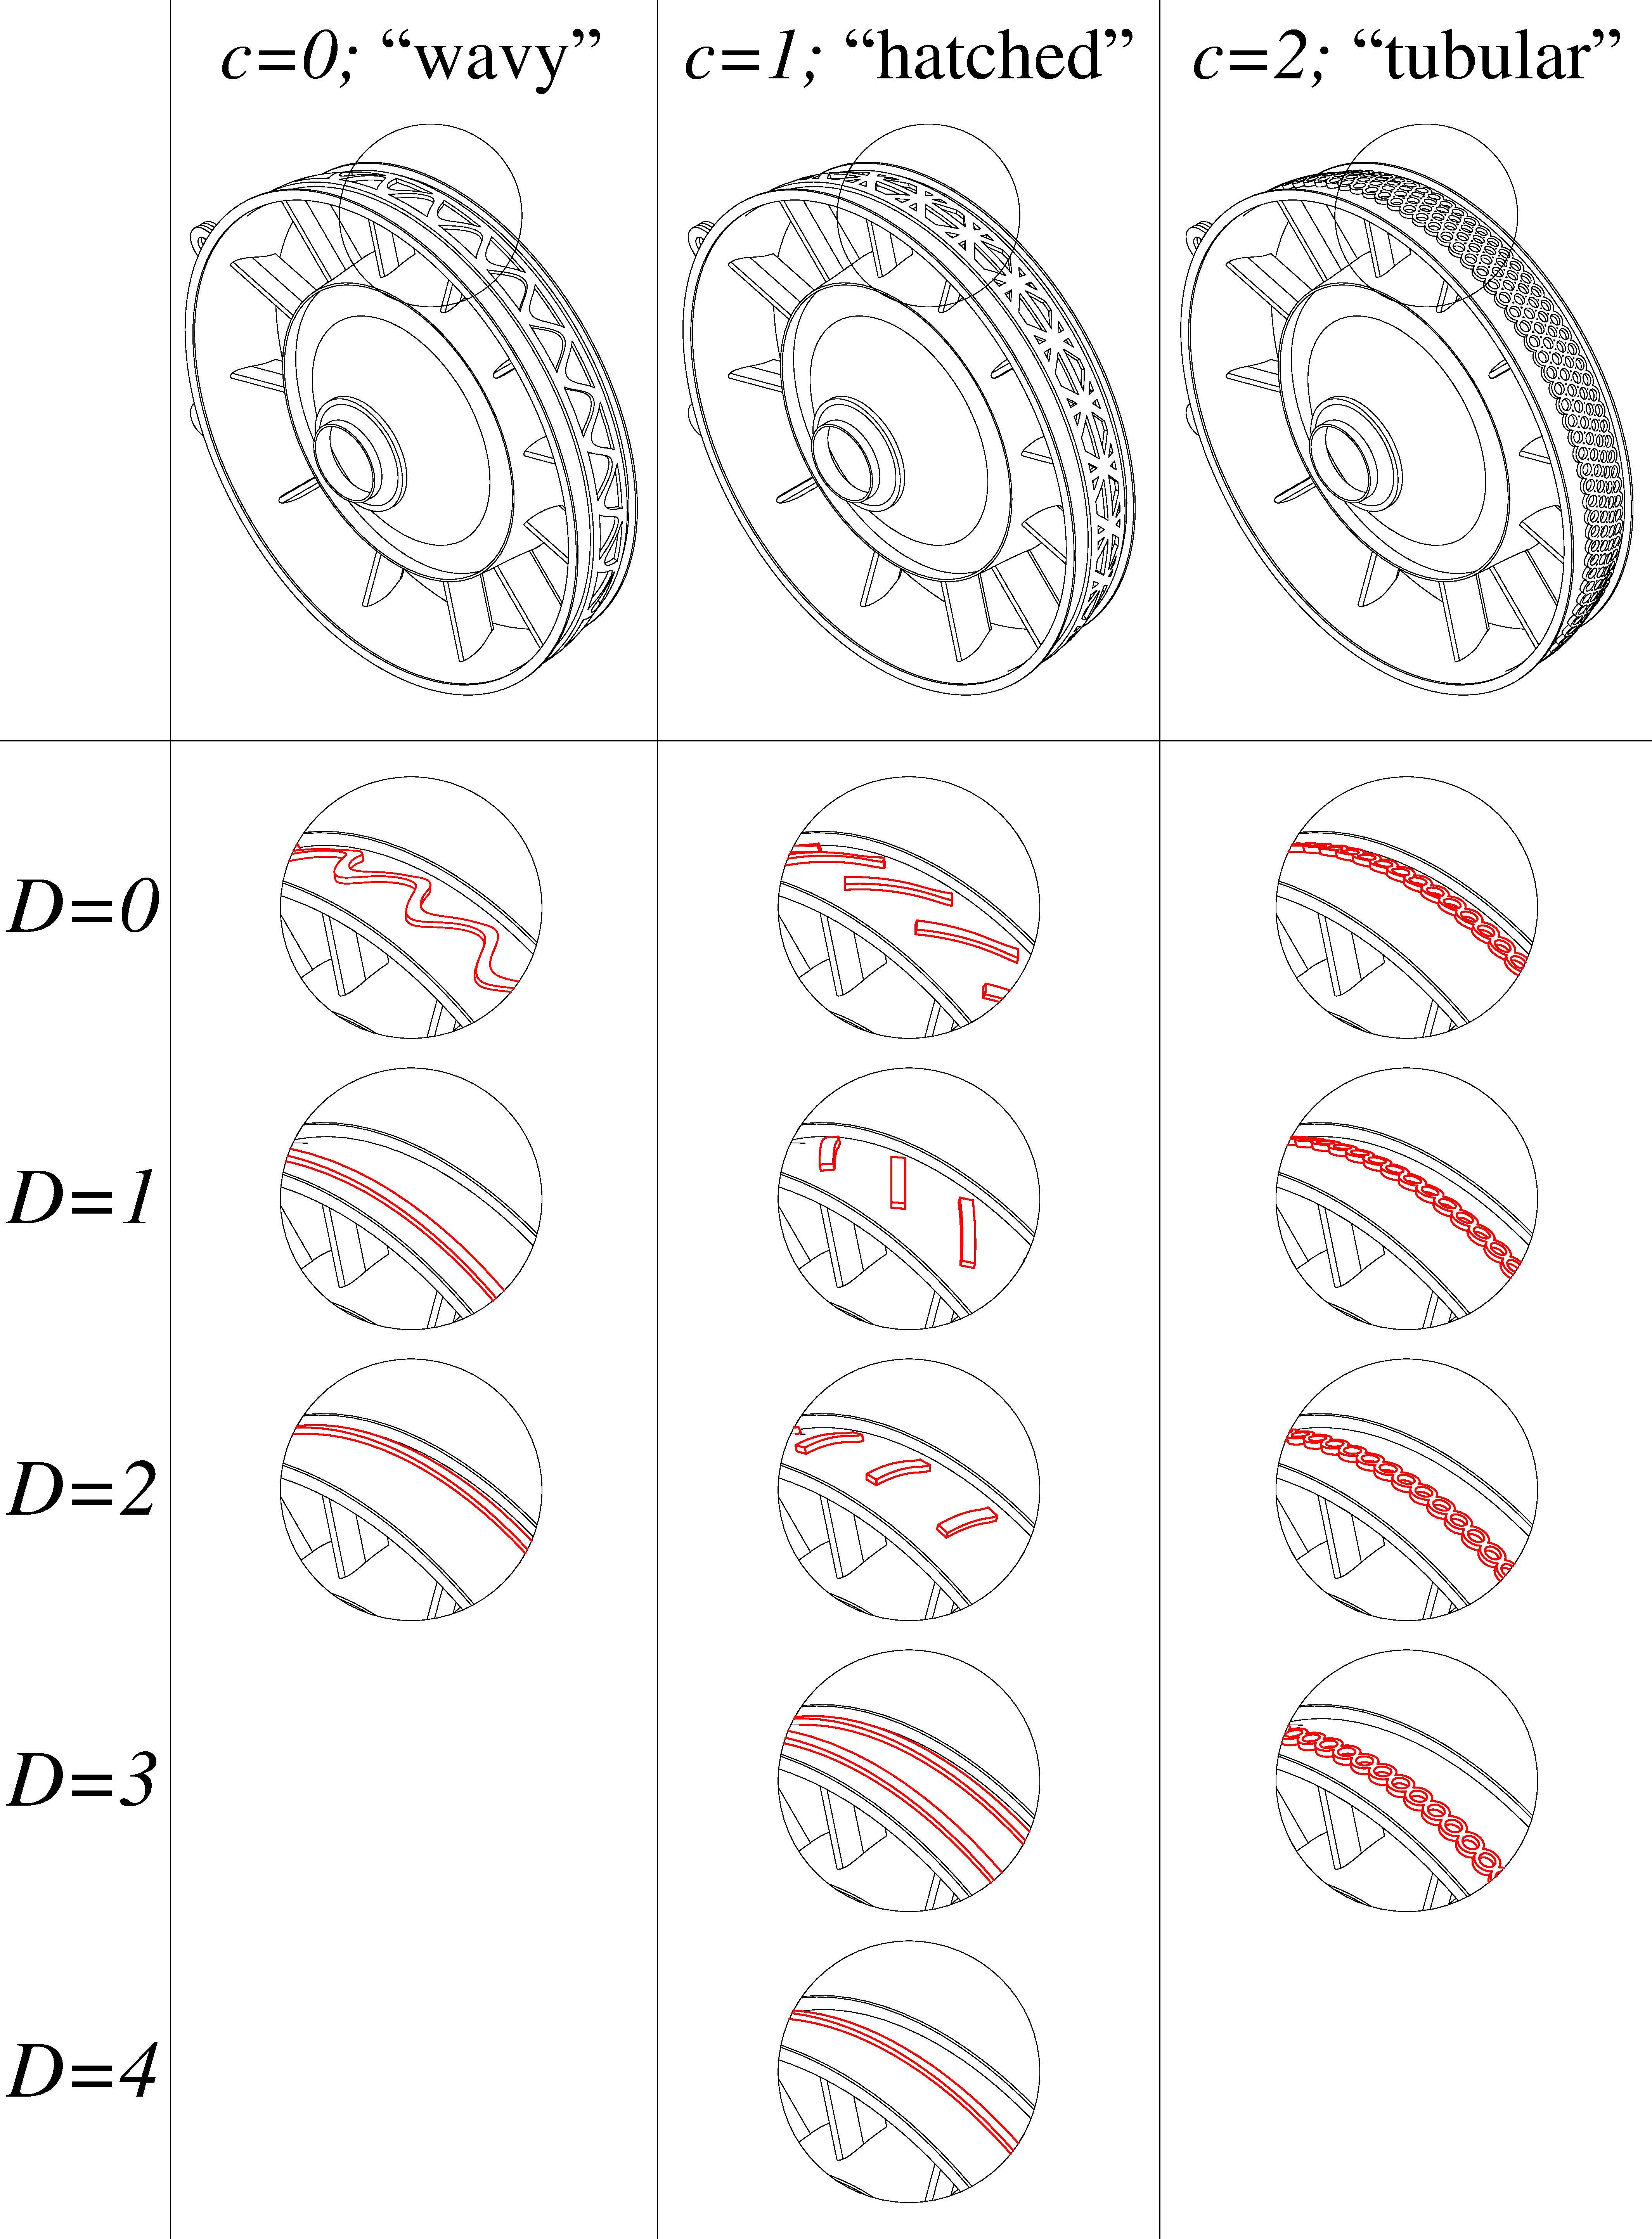
\includegraphics[width=0.6\textwidth]{6_TRS_stiffener_types.pdf}
	\caption{Illustration of possible concepts and redesign choices for \ac{TRS} stiffener}
	\label{fig:designspacestiff}
\end{figure}

We compute the cardinality of the set $\Omega_{cD}$ using Table~\ref{table:omegadcardinality} and Equation~(\ref{eq:cardinailitycdarc}) for this problem as follows:

\begin{equation*}
	\begin{aligned}
		& \mathrm{concept~}c_0:~|\Omega_{D0}| = 15\\
		& \mathrm{concept~}c_1:~|\Omega_{D1}| = 325\\
		& \mathrm{concept~}c_2:~|\Omega_{D2}| = 64\\
		& \beta = |\Omega_{cD}| = 15 + 325 + 64 = 404.\\
	\end{aligned}
\end{equation*}

We now describe the analysis steps for obtaining the capability of a given stiffener design arc as a function of the thermal temperature loads.

%---------------------------------------------------------------------%
% Load case description
\subsection{Loadcase description} \label{subsec:loadcase}

The uncertain temperature loads in Figure~\ref{fig:thermalloads} are used to specify the vector of uncertain parameters given by $\mathbf{p} = \left[T_1 ~ T_2 ~ T_3 ~ T_4\right]^{\mathrm{T}}$ and the corresponding parameter space $\mathbf{p}\in\mathbb{R}^4$, where $n = 4$ is dimensionality of the problem. We constrain our study to a parameter space defined by the following bounds on $\mathbf{p}$.

$\mathbf{p} = \left\{\mathbf{p}: \mathbf{L} \le \mathbf{p} \le \mathbf{U}\right\}$, where $\mathbf{L} = \left[-100 ~ -100 ~ -100 ~ -100\right]^{\mathrm{T}}$ and $\mathbf{U} = \left[100 ~ 100 ~ 100 ~ 100\right]^{\mathrm{T}}$. Note that these bounds are relative to nominal temperature values of $\mathbf{p}_{\textrm{nominal}} = \left[300 ~ 400 ~ 450 ~ 600\right]^{\mathrm{T}}$. A value of $\mathbf{p} = \left[50 ~ 25 ~ -40 ~ -20\right]^{\mathrm{T}} \equiv \mathbf{p} + \mathbf{p}_{\textrm{nominal}} = \left[350 ~ 425 ~ 410 ~ 580\right]^{\mathrm{T}}$.

In this chapter we assume that there is no correlation between these temperature loads. This is because environmental factors such as the atmospheric temperature are independent of the exhaust temperature. This allows us to assume that the requirement \acp{PDF} defined in Section~\ref{subsec:designmetrics} feature diagonal covariance matrices.

The feasibility of a \ac{TRS} design is governed by a single feasibility constraint $g_{f1}(\mathbf{p}) - t_1 \le 0$. For this problem, $g_{f1}(\mathbf{p}) = -n_{\textrm{safety}}(\mathbf{p})$ which is the safety factor of the design against low-cycle fatigue failure or yielding whichever comes first and is computed by a structural analysis model following the thermomechanical analysis of the stiffener deposition. $t_1 = -2.8$ is the threshold safety factor that defines feasibility. The safety factor $n_{\textrm{safety}}(\mathbf{p})$ is computed using the procedure in Section \ref{subsec:fatigueanalysis}. Note that the safety factor $n_{\textrm{safety}}(\mathbf{p})$ for a particular stiffener design arc is dependant on the applied temperature loads $(\mathbf{p})$.

For every design arc in $\Omega_{cD}$, we construct a surrogate model for computing $n_{\textrm{safety}}(\mathbf{p})$. The surrogate is constructed by training a response surface model from data obtained from the simulation model. 25 \ac{LH} samples from the parameter space are used as training data for the response surface. We use an open source surrogate model library to build and optimize the hyperparameters of an ensemble of surrogates \cite{Talgorn2018}. This results in a surrogate for the feasibility constraint $\hat{g}_{f1}(\mathbf{p}) - t_1 \le 0$. We visualize this feasibility constraint on the 4-dimensional parameter space for a few example design arcs in Section~\ref{subsec:exampleprob4D}. 

%---------------------------------------------------------------------%
% Load case requirements
\subsection{Loadcase requirements} \label{subsec:loadcasereq}

Having defined the 4-dimensional parameter space, we can now define the requirement joint \acp{PDF} that will be used and the corresponding requirement arcs that can be constructed from them. 

Two types of requirement joint \acp{PDF} will be used, the uniform distribution and the Gaussian distribution given by Equations~(\ref{eq:uniformpdf}) and (\ref{eq:gaussianpdf}) respectively. As a result, $\mathcal{T} = \left\{\mathrm{``Uniform"},\mathrm{``Gaussian"}\right\}$.

All design metrics and requirements are calculated for uncertain parameter spaces that are scaled between $0$ and $1$. This helps when making comparisons between different design arcs in terms of hypervolume of sets with $0$ being the minimum possible hypervolume and $1$ being the maximum possible hypervolume.

$e=5$ interpolation levels are used to obtain $M$ and $\boldsymbol{\Sigma}$. The starting mean and interval vectors are $\boldsymbol{\mu}_1 = \left[0.15 ~ 0.80 ~ 0.80 ~ 0.85\right]^{\mathrm{T}}$ and $\boldsymbol{\sigma}_1 = \left[0.1875 ~ 0.125 ~ 0.125 ~ 0.1875\right]^{\mathrm{T}}$ respectively. The ending mean and interval vectors are $\boldsymbol{\mu}_5 = \left[0.85 ~ 0.20 ~ 0.20 ~ 0.15\right]^{\mathrm{T}}$ and $\boldsymbol{\sigma}_5 = \left[0.375 ~ 0.250 ~ 0.250 ~ 0.375\right]^{\mathrm{T}}$ respectively. As a result, the set of mean and interval vectors is given by:

% \begin{equation*}
% 	M = \begin{Bmatrix} 
% 		[ & 0.15 & 0.80 & 0.80 & 0.85 & ],\\ 
% 		[ & 0.325 & 0.65 & 0.65 & 0.675 & ],\\
% 		[ & 0.5 & 0.5 & 0.5 & 0.5 & ],\\
% 		[ & 0.675 & 0.35 & 0.35 & 0.325 & ],\\
% 		[ & 0.85 & 0.20 & 0.20 & 0.15 & ]
% 	 \end{Bmatrix},
% \end{equation*}

% and \begin{equation*}
% 	\Sigma = \begin{Bmatrix} 
% 		[ & 0.1875 & 0.125 & 0.125 & 0.1875 & ],\\ 
% 		[ & 0.234375 & 0.15625 & 0.15625 & 0.234375 & ],\\
% 		[ & 0.28125 & 0.1875 & 0.1875 & 0.28125 & ],\\
% 		[ & 0.328125 & 0. & 0.21875 & 0.328125 & ],\\
% 		[ & 0.375 & 0.250 & 0.250 & 0.375 & ]
% 	 \end{Bmatrix}
% \end{equation*}

\begin{equation*}
	M = \left\{ \begin{aligned}
		& \left[ 0.15 ~ 0.80 ~ 0.80 ~ 0.85 \right]^{\mathrm{T}},\\ 
		& \left[ 0.325 ~ 0.65 ~ 0.65 ~ 0.675 \right]^{\mathrm{T}},\\
		& \left[ 0.5 ~ 0.5, 0.5 ~ 0.5 \right]^{\mathrm{T}},\\
		& \left[ 0.675 ~ 0.35 ~ 0.35 ~ 0.325 \right]^{\mathrm{T}},\\
		& \left[ 0.85 ~ 0.20 ~ 0.20 ~ 0.15 \right]^{\mathrm{T}},
	\end{aligned} \right\}
\end{equation*}

and

\begin{equation*}
	\Sigma = \left\{ \begin{aligned}
		& \left[ 0.1875 ~ 0.125 ~ 0.125 ~ 0.1875 \right]^{\mathrm{T}},\\ 
		& \left[ 0.234375 ~ 0.15625 ~ 0.15625 ~ 0.234375 \right]^{\mathrm{T}},\\
		& \left[ 0.28125 ~ 0.1875 , 0.1875 ~ 0.28125 \right]^{\mathrm{T}},\\
		& \left[ 0.328125 ~ 0.21875 ~ 0.21875 ~ 0.328125 \right]^{\mathrm{T}},\\
		& \left[ 0.375 ~ 0.250 ~ 0.250 ~ 0.375 \right]^{\mathrm{T}}
	\end{aligned} \right\}
\end{equation*}

respectively.

We define a remanufacturing design problem with $m = 6$ epochs. The number of choices $v$ for $\mathcal{R} = \left\{F_{\mathbf{X}1}(\mathbf{p}),F_{\mathbf{X}2}(\mathbf{p}),\cdots,F_{\mathbf{X}v}(\mathbf{p})\right\}$ and the cardinality $s$ for $\Omega_R$ is calculated as follows:

\begin{equation*}
	\begin{aligned}
		& v = e \times e \times |\mathcal{T}| = 5 \times 5 \times 2 = 50,\\
		& s = |\Omega_R| = m^v = 6^{50},~\mathrm{respectively}.\\
	\end{aligned}
\end{equation*}

Only the first few elements of $\Omega_R$ will be used during the set-based design analysis and $s$ will be capped at $10^5$ samples. This is because the set-based solutions stabilize and do not change after sampling $10^3$ requirement arc samples.

The reliability threshold vector for this application problem is defined as 

\begin{equation*}
    \mathbf{P}_{th} = \left[0.01 ~ 0.1 ~ 0.3 ~ 0.3 ~ 0.8 ~ 0.9\right]^{\mathrm{T}}.
\end{equation*}

The reliability threshold gradually increases as a product development cycle progresses. This is in contrast to the reliabilities encountered during a product's lifecycle where the reliability is generally high in aerospace industries. The designer can test and react to different lifecycle scenarios by adjusting the reliability threshold for the problem.

We now summarize the important problem parameters and constants in Table~\ref{table:modelsummary}.

\begin{table}[h!]
	\centering
	\renewcommand{\arraystretch}{1.0}% Wider
	\footnotesize\addtolength{\tabcolsep}{-5pt}
	\caption{Relevant model parameters and constants}
	\label{table:modelsummary}
	\begin{tabular}{lcc>{\centering\arraybackslash}p{4cm}}
	\hline\hline
	\bf Parameter/constant & \bf Notation & \bf Units & \bf Nominal value \\
	\hline
	%================================================================
	Concept choices & $\mathcal{C}$ & - & $\left\{0,1,2\right\}$ \\
	Deposit choices for concept 0 & $\mathcal{D}_0$ & - & $\left\{0,1,2\right\}$ \\
	Deposit choices for concept 1 & $\mathcal{D}_1$ & - & $\left\{0,1,2,3,4\right\}$ \\
	Deposit choices for concept 2 & $\mathcal{D}_2$ & - & $\left\{0,1,2,3\right\}$ \\
	Cardinality of design arcs & $\beta$ & - & 404  \\
	Number of epochs & $m$ & - & 6 \\
	Interpolation levels & $e$ & - & 5 \\
	\ac{PDF} types & $\mathcal{T}$ & - & $\left\{\mathrm{``Uniform"},\mathrm{``Gaussian"}\right\}$ \\
	\ac{PDF} starting mean & $\boldsymbol{\mu}_1$ & - & $\left[0.15 ~ 0.80 ~ 0.80 ~ 0.85\right]^{\mathrm{T}}$ \\
	\ac{PDF} starting interval & $\boldsymbol{\sigma}_1$ & - & $\left[0.1875 ~ 0.125 ~ 0.125 ~ 0.1875\right]^{\mathrm{T}}$ \\
	\ac{PDF} ending mean & $\boldsymbol{\mu}_e$ & - & $\left[0.85 ~ 0.20 ~ 0.20 ~ 0.15\right]^{\mathrm{T}}$ \\
	\ac{PDF} ending interval & $\boldsymbol{\sigma}_e$ & - & $\left[0.375 ~ 0.250 ~ 0.250 ~ 0.375\right]^{\mathrm{T}}$ \\
	Reliability threshold & $\mathbf{P}_{th}$ & - & $\left[0.01 ~ 0.1 ~ 0.3 ~ 0.3 ~ 0.8 ~ 0.9\right]^{\mathrm{T}}$ \\
	Number of requirement \acp{PDF} & $v$ & - & 50 \\
	Number of requirement arc samples & $s$ & - & $10^5$ \\ \hline
	%================================================================
	Nacelle temperature & $T_1$ & $^{o}$C & $300 \pm 100$ \\ 
	Tailcone temperature & $T_2$ & $^{o}$C & $400 \pm 100$ \\ 
	Rotor temperature & $T_3$ & $^{o}$C & $450 \pm 100$ \\ 
	Gas surface temperature & $T_4$ & $^{o}$C & $600 \pm 100$ \\
	Parameter vector & $\mathbf{p}$ & - & $\left[T_1 ~ T_2 ~ T_3 ~ T_4\right]^{\mathrm{T}}$ \\ \hline
	%================================================================
	Laser Power & ${P_\textrm{laser}}$ & W &  3806 \\ 
	Laser beam radius & ${r_l}$ & mm & 14.2 \\ 
	Scanning speed& ${V}$ & mm/s & 5.0 \\ 
	Stiffener height & $S_\textrm{height}$ & mm & 10.0 \\
	Laser penetration depth & $D_p$ & mm & 5.0 \\
	Number of deposition layers & $n_d$ & - & 2 \\
	Threshold low-cycle fatigue safety factor & $t_1$ & - & -2.8 \\
	%================================================================
	\hline\hline
	\end{tabular}
\end{table}

%============================ RESULTS ============================%
\section{Results and discussion} \label{sec:TSEresults}

% {\color{red} Here we describe the obtained results in the context of a tradespace and comment on the most frequent deposit type encountered during the first stage. This helps designers choose a good starting point that will allow room to evolve to meet the largest number of possible requirement profiles likely to be encountered in the future}

We investigate the remanufacturing design problem of a \ac{TRS} by using the surrogate thermomechanical/structural analysis to obtain the capability set for every design arc in the set $\Omega_{cD}$. We begin by investigating a few select design arcs from $\Omega_{cD}$. We then solve a single combinatorial optimization problem to minimize excess for a given requirement arc from the set $\Omega_R$. We then present the set-based results for the problem using a tradespace.

%---------------------------------------------------------------------%
% Example calculation
\subsection{Example for calculating the design properties of a given design arc} \label{subsec:exampleprob4D}

The requirements are defined in the parameter space by either a uniform or Gaussian \ac{PDF} as given by Equations~(\ref{eq:uniformpdf}) and (\ref{eq:gaussianpdf}) respectively. We choose two design arcs from the set $\Omega_{cD}$ to visualize their feasibility constraints, capabilities and reliabilities in the 4-dimensional parameter space in Figure~\ref{fig:4Dexamplepspace}. The design arcs and their filtered outdegree, weight and hypervolume of capability are reported in Table~\ref{table:pdf4Dexample}. Additionally, two different requirement joint \acp{PDF} are specified and the corresponding reliability, hypervolume of requirement and hypervolume of excess are reported in Table~\ref{table:pdf4Dexample}.

\newcommand{\cwaa}{0.75cm} % index column width
\newcommand{\cwa}{1.5cm} % design arc column width
\newcommand{\cwc}{1.5cm} % FO column width
\newcommand{\cwd}{1cm} % FO column width
\newcommand{\cwe}{1.5cm} % mean column width
\newcommand{\cwf}{1.5cm} % interval column width
%
%
\newcommand{\cwb}{1.1cm} % Capability column width
\newcommand{\cwi}{1.1cm} % R volume column width
\newcommand{\cwj}{1.1cm} % E volume column width

\begin{table}[h!]
	\centering
	% \renewcommand{\arraystretch}{1.0}% Wider
	\footnotesize\addtolength{\tabcolsep}{-5pt}
	\caption{Results obtained for example design arcs and requirement joint \acp{PDF}}
	\label{table:pdf4Dexample}
	\begin{tabular}{>{\centering\arraybackslash}p{\cwaa}>{\centering\arraybackslash}p{\cwa}|>{\centering\arraybackslash}p{\cwc}c>{\centering\arraybackslash}p{\cwe}>{\centering\arraybackslash}p{\cwf}cc>{\centering\arraybackslash}p{\cwi}>{\centering\arraybackslash}p{\cwj}>{\centering\arraybackslash}p{\cwb}}
	\hline\hline
	\bf Index & \bf Design arc & \bf Filtered outdegree & \bf Weight &\bf \ac{PDF} mean vector & \bf \ac{PDF} interval vector & \bf \ac{PDF} type & \bf Reliability & \multicolumn{3}{c}{\bf Set volume} \\
	$\lambda$ & $\left\{c,\mathbf{D}\right\}$ & $FO$ & $W$ &$\boldsymbol{{\mu}}$ & $\boldsymbol{{\sigma}}$ & $t$ & $\mathbb{P}\left(\mathbf{p}\in C\right)$ & $V_R$ & $V_E$ & $V_C$ \\ \hline
	%================================================================
	\multirow{5}{\cwaa}{\centering 109} & & \multirow{5}{\cwc}{\centering 2} & \multirow{5}{\cwd}{\centering 13.9 kg} & \multirow{5}{\cwe}{\centering $\begin{bmatrix} 0.375 \\ 0.5 \\ 0.5 \\0.625 \end{bmatrix}$} & \multirow{5}{\cwf}{\centering $\begin{bmatrix} 0.375 \\ 0.125 \\ 0.125 \\0.375 \end{bmatrix}$} & & & & & \multirow{5}{\cwb}{\centering 0.540} \\
	 & $\{c = 1,$ & & & & & ``Uniform" & 0.3089 & 0.0352 & 0.529 \\
	 & $\mathbf{D} = \left[1,2,4\right]\}$ & & & & & & & & & \\
	 & & & & & & ``Gaussian" & 0.165 & 0.0108 & 0.540\\
	 & & & & & & & & & & \\ \hline
	%================================================================
	\multirow{5}{\cwaa}{\centering 110} & & \multirow{5}{\cwc}{\centering 1} & \multirow{5}{\cwd}{\centering 18.5 kg} & \multirow{5}{\cwe}{\centering $\begin{bmatrix} 0.375 \\ 0.5 \\ 0.5 \\0.625 \end{bmatrix}$} & \multirow{5}{\cwf}{\centering $\begin{bmatrix} 0.375 \\ 0.125 \\ 0.125 \\0.375 \end{bmatrix}$} & & & & & \multirow{5}{\cwb}{\centering 0.883} \\
	 & $\{c = 1,$ & & & & & ``Uniform" & 0.759 & 0.0352 & 0.856 \\
	 & $\mathbf{D} = \left[1,2,4,0\right]\}$ & & & & & & & & & \\
	 & & & & & & ``Gaussian" & 0.908 & 0.0108 & 0.875 \\
	 & & & & & & & & & & \\
	%================================================================
	\hline\hline
	\end{tabular}
\end{table}

We can see from the results in Table~\ref{table:pdf4Dexample} that the addition of one more deposits to the design arc $\left\{c = 1, \mathbf{D} = \left[1,2,4\right]\right\}$ increases its performance in terms of capability and reliability. However, this comes at the increased cost of an additional 4.6 kg of weight, reduced filtered outdegree and an additional excess of 0.327 and 0.335 for uniform and Gaussian \acp{PDF} respectively. The choice of design arc for a given requirement arc is driven by the need to maintain a minimum reliability while minimizing excess. We will look at such a problem using epoch era analysis and combinatorial optimization for decision making.

\begin{figure}[h!]
	\centering
	\subfloat[{$\left\{c = 1,\mathbf{D} = \left[1,2,4\right]\right\}$}\label{fig:darc1R1}]{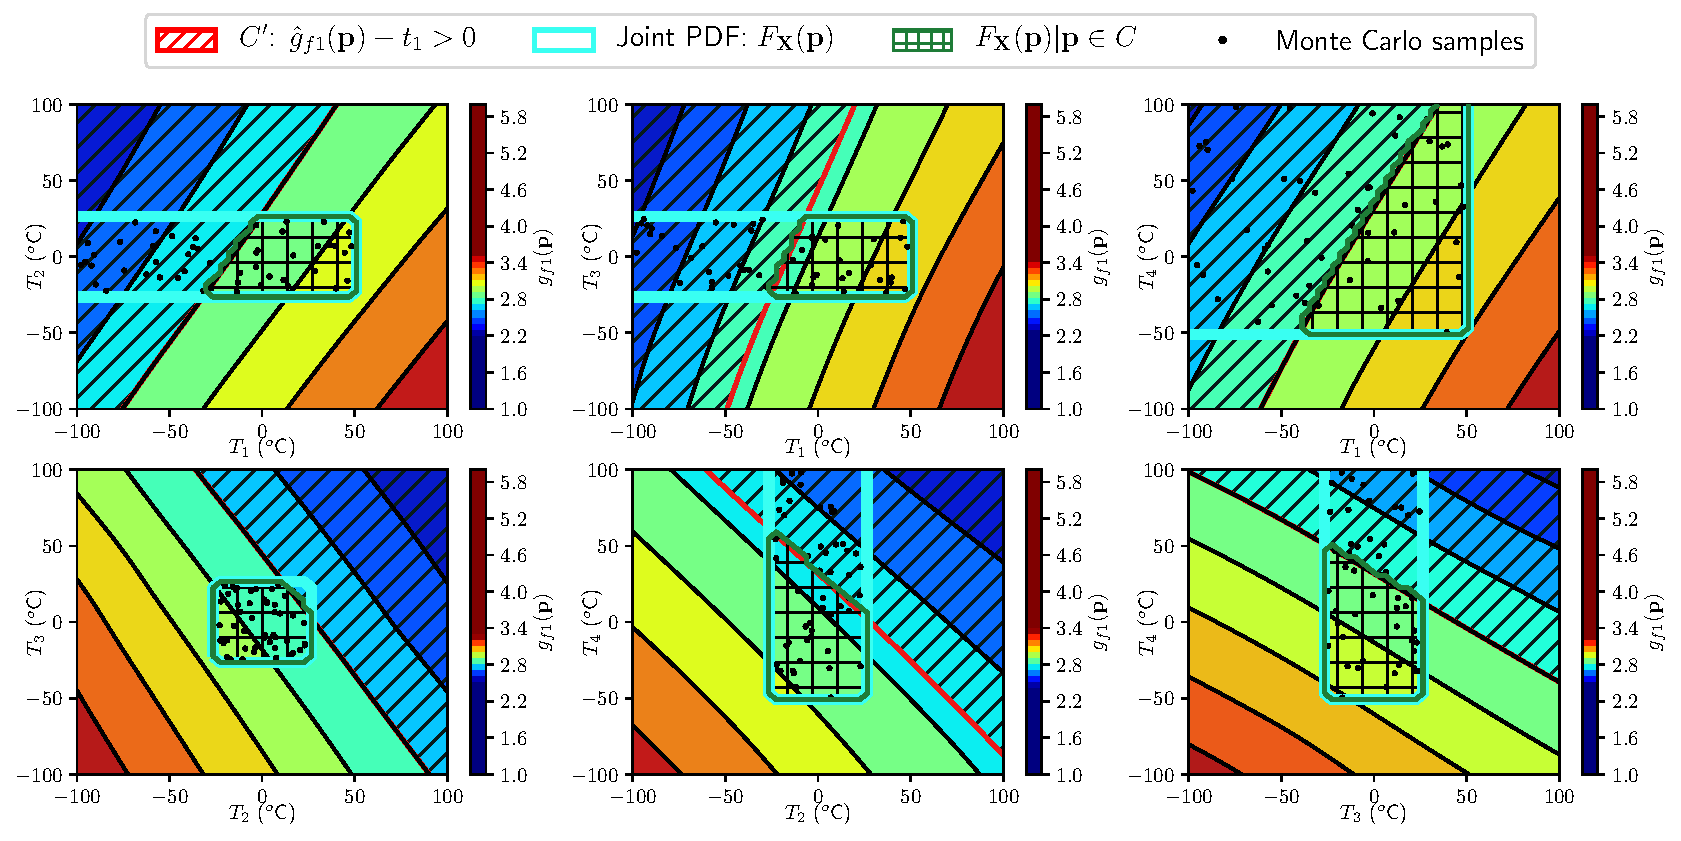
\includegraphics[width=0.9\textwidth]{8a_thermal_out_nominal_RS}}
	
	\subfloat[{$\left\{c = 1,\mathbf{D} = \left[1,2,4,0\right]\right\}$} \label{fig:darc2R1}]{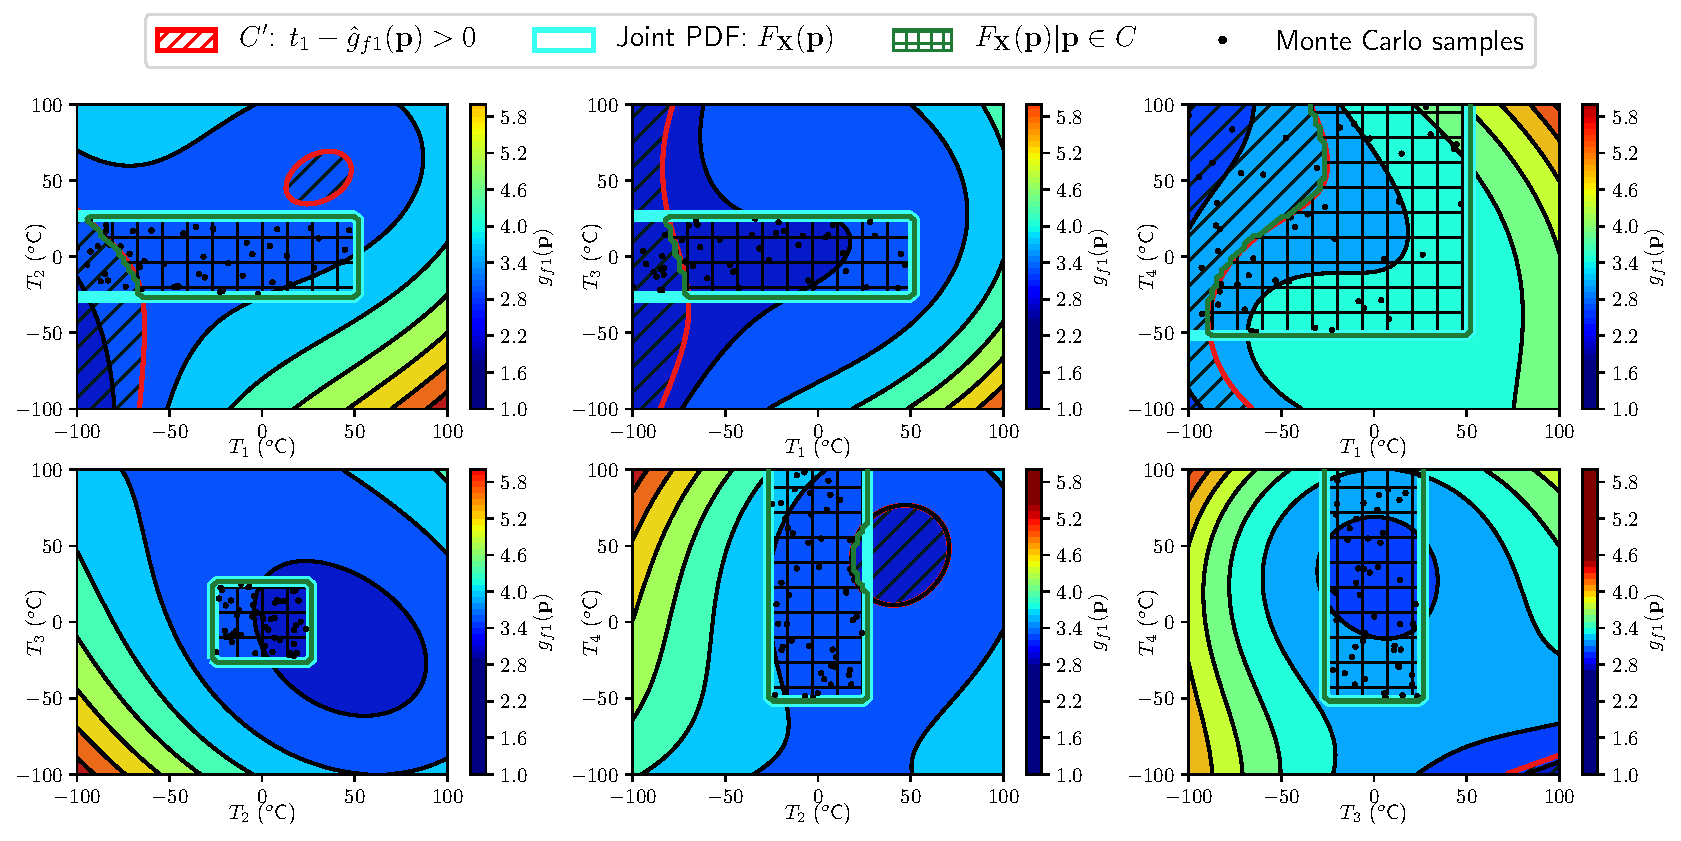
\includegraphics[width=0.9\textwidth]{8b_thermal_out_nominal_RS}}
	\caption{2D projections of the parameter space $\mathbf{p} \in \mathbb{R}^4$}
	\label{fig:4Dexamplepspace}
\end{figure}

%---------------------------------------------------------------------%
% Example calculation
\subsection{Combinatorial optimization with respect to a requirement arc} \label{subsec:exampleoptprob}

We solve the problem given by Equation~(\ref{eq:TSEoptproblem}) using \ac{MADS} for mixed variable problems \cite{Abramson2009}. The requirement arc $\mathbf{R}_w$ used for this problem is given in Table~\ref{table:requirementarcex}. The probability threshold used to define the relaibility constraints is given as

\begin{equation*}
    \mathbf{P}_{th} = \left[0.01~0.1~0.3~0.3~0.8~0.9\right]^{\mathrm{T}}.
\end{equation*}

\begin{table}[h!]
	\centering
	\renewcommand{\arraystretch}{1.0}% Wider
	\footnotesize\addtolength{\tabcolsep}{-5pt}
	\caption{Requirement arc $\mathbf{R}_w$ details}
	\label{table:requirementarcex}
	\begin{tabular}{l>{\centering\arraybackslash}p{4.2cm}>{\centering\arraybackslash}p{6cm}c}
	\hline\hline

	\bf \ac{PDF} Index & \bf \ac{PDF} mean vector & \bf \ac{PDF} interval vector & \bf \ac{PDF} type \\
	$F_\mathbf{X} \in \mathcal{R}$ &$\boldsymbol{{\mu}}$ & $\boldsymbol{{\sigma}}$ & $t$ \\ \hline

	\hline
	%================================================================
	$F_{\mathbf{X36}}$ & $\begin{bmatrix} 0.5 & 0.5 & 0.5 & 0.5 \end{bmatrix}$ & $\begin{bmatrix} 0.1875 & 0.125 & 0.125 & 0.1875 \end{bmatrix}$ & "Gaussian" \\
	$F_{\mathbf{X50}}$ & $\begin{bmatrix} 0.85 & 0.2 & 0.2 & 0.15 \end{bmatrix}$ & $\begin{bmatrix} 0.375 & 0.25 & 0.25 & 0.375 \end{bmatrix}$ & "Gaussian" \\
	$F_{\mathbf{X1}}$ & $\begin{bmatrix} 0.15 & 0.8 & 0.8 & 0.85 \end{bmatrix}$ & $\begin{bmatrix} 0.1875 & 0.125 & 0.125 & 0.375 \end{bmatrix}$ & "uniform" \\
	$F_{\mathbf{X46}}$ & $\begin{bmatrix} 0.85 & 0.2 & 0.2 & 0.15 \end{bmatrix}$ & $\begin{bmatrix} 0.1875 & 0.125 & 0.125 & 0.1875 \end{bmatrix}$ & "Gaussian" \\
	$F_{\mathbf{X13}}$ & $\begin{bmatrix} 0.5 & 0.5 & 0.5 & 0.5 \end{bmatrix}$ & $\begin{bmatrix} 0.28125 & 0.1875 & 0.1875 & 0.28125 \end{bmatrix}$ & "uniform" \\
	$F_{\mathbf{X31}}$ & $\begin{bmatrix} 0.325 & 0.65 & 0.65 & 0.675 \end{bmatrix}$ & $\begin{bmatrix} 0.1875 & 0.125 & 0.125 & 0.1875 \end{bmatrix}$ & "Gaussian" \\
	%================================================================
	\hline\hline
	\end{tabular}
\end{table}

We plot the results from various decision arcs across epochs in Figure~\ref{fig:epocheraexample}. The first decision arc, $c=1,\mathbf{S}=\left[2,1,-1,-1,0,-1\right]$ (shown in red) does not satisfy the reliability constraints for the problem as shown in Figure~\ref{fig:Decisionarcreliability}. This is because at epoch $k=3$ the reliability of the corresponding design arc $c=1,\mathbf{D}=\left[2,1\right]$ is almost 0. No redesign occurred at epoch $k=3$ when it was needed to increase the reliability of the design arc above the threshold.

We investigate another decision arc $c=1,\mathbf{S}=\left[4,1,0,2,-1,3\right]$ (shown in green) that achieves very high reliability throughout all epochs. However, this comes at the cost of increased cumulative excess (green shaded area under excess/epoch graph) relative to that of the first decision arc (shown in as the red shaded area) in Figure~\ref{fig:Decisionarcexcess}.

we solve the combinatorial problem given by Equation~(\ref{eq:TSEoptproblem}) to get the third decision arc $c=1,\mathbf{S}=\left[4,1,0,2,-1,3\right]$ (shown in blue) which is optimal in terms of minimizing excess. This decision arc has lower reliability relative to the second decision arc (shown in green) but lower cumulative excess and therefore less overdesign. We provide the values of the objective function and reliability constraints for all three decision arcs in Table~\ref{table:optresults}.

\begin{figure}[h!]
	\centering
	\subfloat[Reliability over multiple epochs \label{fig:Decisionarcreliability}]{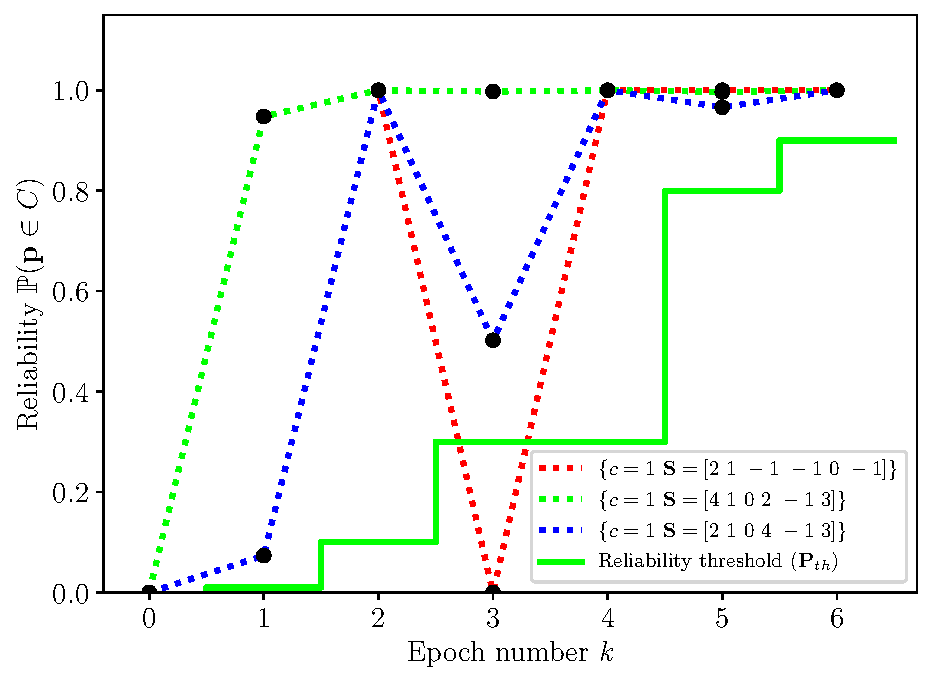
\includegraphics[width=0.45\textwidth]{10a_stagespace_res}} \hspace{0.1\textwidth}%
	\subfloat[Volume of excess set over multiple epochs \label{fig:Decisionarcexcess}]{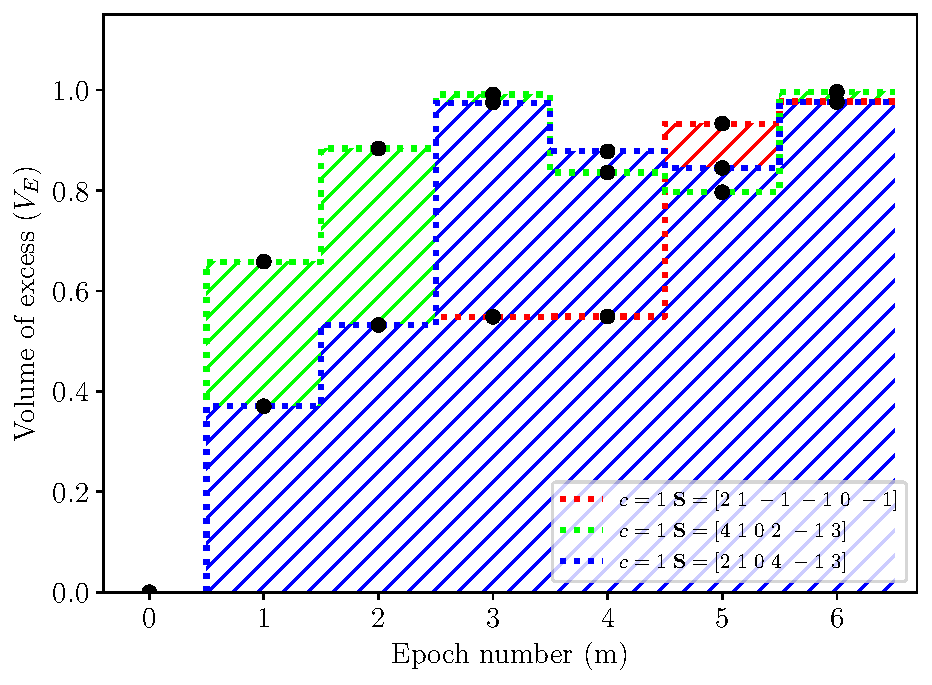
\includegraphics[width=0.45\textwidth]{10b_stagespace_obj}} \hspace{0.1\textwidth}%	
	\caption{Visualization of several decision arcs}
	\label{fig:epocheraexample}
\end{figure}

\newcommand{\ocwa}{0.75cm} % index column width
\newcommand{\ocwb}{3cm} % decision arc column width
\newcommand{\ocwc}{1.5cm} % objective column width
\newcommand{\ocwd}{2cm} % constraints column width
\newcommand{\ocwe}{3cm} % design arc column width

\begin{table}[h!]
	\centering
	% \renewcommand{\arraystretch}{1.0}% Wider
	\footnotesize\addtolength{\tabcolsep}{-5pt}
	\caption{Results obtained for example design arcs and requirement joint \acp{PDF}}
	\label{table:optresults}
	\begin{tabular}{>{\centering\arraybackslash}p{\ocwa}>{\centering\arraybackslash}p{\ocwb}|>{\centering\arraybackslash}p{\ocwc}>{\centering\arraybackslash}p{\ocwd}>{\centering\arraybackslash}p{\ocwe}}
	\hline\hline
	\bf Index & \bf Decision arc & \bf Objective value & \bf Reliability constraints & \bf Design arc \\ & $\left\{c,\mathbf{S}\right\}$ & $f(c,\mathbf{S};\mathbf{R})$ & $\mathbf{g}(c,\mathbf{S};\mathbf{R})$ & $\left\{c,\mathbf{D}\right\}$ \\ \hline
	%================================================================
	\multirow{6}{\ocwa}{\centering 1} & \multirow{6}{\ocwb}{\centering $c=1,\mathbf{S}=\left[2,1,-1,-1,0,-1\right]$} & \multirow{6}{\ocwc}{\centering 3.91} & \multirow{6}{\ocwd}{\centering $\begin{bmatrix} -0.063 \\ -0.9 \\ 0.3 \\ -0.7 \\ -0.2 \\ -0.1 \end{bmatrix}$} & \multirow{6}{\ocwd}{\centering $c=1,\mathbf{D}=\left[2,1,0\right]$} \\
	 & & & & \\
	 & & & & \\
	 & & & & \\
	 & & & & \\
	 & & & & \\ \hline
	%================================================================
	\multirow{6}{\ocwa}{\centering 2} & \multirow{6}{\ocwb}{\centering $c=1,\mathbf{S}=\left[4,1,0,2,-1,3\right]$} & \multirow{6}{\ocwc}{\centering 5.16} & \multirow{6}{\ocwd}{\centering $\begin{bmatrix} -0.94 \\ -0.9 \\ -0.70 \\ -0.7 \\ -0.20 \\ -0.1 \end{bmatrix}$} & \multirow{6}{\ocwd}{\centering $c=1,\mathbf{D}=\left[4,1,0,2,3\right]$} \\
	& & & & \\
	& & & & \\
	& & & & \\
	& & & & \\
	& & & & \\ \hline
	%================================================================
	\multirow{6}{\ocwa}{\centering 3} & \multirow{6}{\ocwb}{\centering $c=1,\mathbf{S}=\left[2,1,0,4,-1,3\right]$} & \multirow{6}{\ocwc}{\centering 4.58} & \multirow{6}{\ocwd}{\centering $\begin{bmatrix} -0.063 \\ -0.9 \\ -0.20 \\ -0.7 \\ -0.17 \\ -0.1 \end{bmatrix}$} & \multirow{6}{\ocwd}{\centering $c=1,\mathbf{D}=\left[2,1,0,4,3\right]$} \\
	& & & & \\
	& & & & \\
	& & & & \\
	& & & & \\
	& & & & \\
	%================================================================
	\hline\hline
	\end{tabular}
\end{table}

Finally, the example in this section shows that the order of redesign steps can have a significant impact on the reliability and level of overdesign throughout epochs. The second and third decision arcs contain the same redesign choices but in different order. The differences between them in terms of reliability and cumulative excess reflect the importance of choosing the right order of redesign operations when considering multiple epochs.

We will now solve similar combinatorial optimization problems for every requirement arc in the set $\Omega_R$ to obtain a set-based solution.

%---------------------------------------------------------------------%
% Example calculation
\subsection{Set-based design and tradespace exploration} \label{subsec:SBDTSE}

We solve an optimization problem similar to the one in Section~\ref{subsec:exampleoptprob} for every requirement arc in $\Omega_R$ to obtain the set of parametric optimal design arcs when optimizing for cumulative excess ($S_E^*$) and cumulative weight ($S_W^*$). We plot the frequency of each design arc in $S_E^*$ and $S_W^*$ and normalize it by the cardinality $\beta$ of set $\Omega_R$ to obtain the histograms shown in Figure~\ref{fig:histogramplotsSBD}. 

We also evaluated the flexibility and robustness of each design arc in $\Omega_{cD}$ using the methodology in Figure~\ref{fig:methodology}. We present the set of design arcs ordered with respect to robustness and flexibility in Figures~\ref{fig:histogramR} and \ref{fig:histogramF} respectively.

\begin{figure}[h!]
	\centering
	\subfloat[Objective: minimize cumulative excess\label{fig:histogramSBDE}]{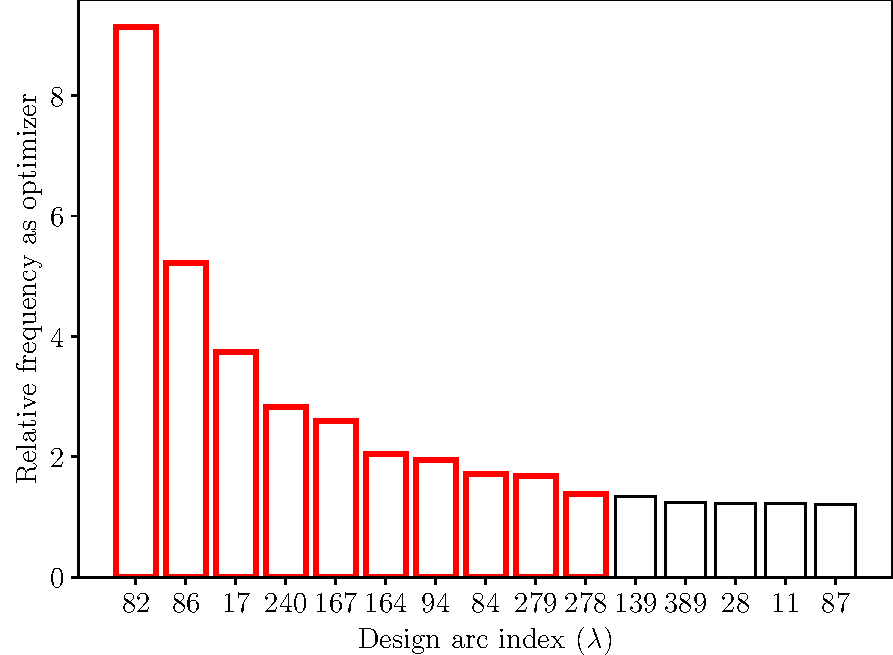
\includegraphics[width=0.45\textwidth]{11a_histogram_DOE_E}} \hspace{0.1\textwidth}%
	\subfloat[Objective: minimize cumulative weight\label{fig:histogramSBDW}]{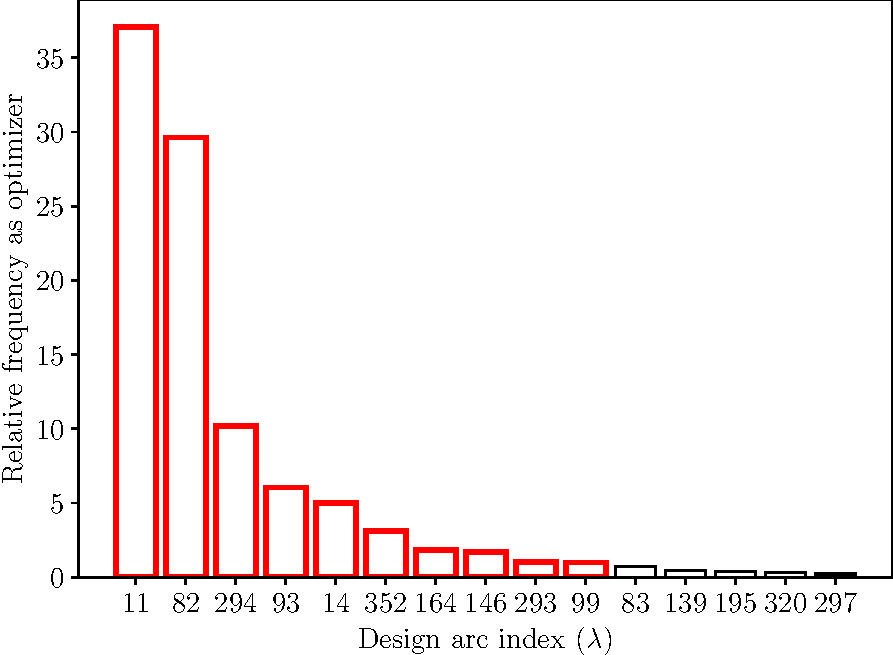
\includegraphics[width=0.45\textwidth]{11b_histogram_DOE_W}} \hspace{0.1\textwidth}%	
	\caption{Distribution of design arcs in optimization driven set-based solutions}
	\label{fig:histogramplotsSBD}
\end{figure}

\begin{figure}[h!]
	\centering
	\subfloat[Set of robust design arcs \label{fig:histogramR}]{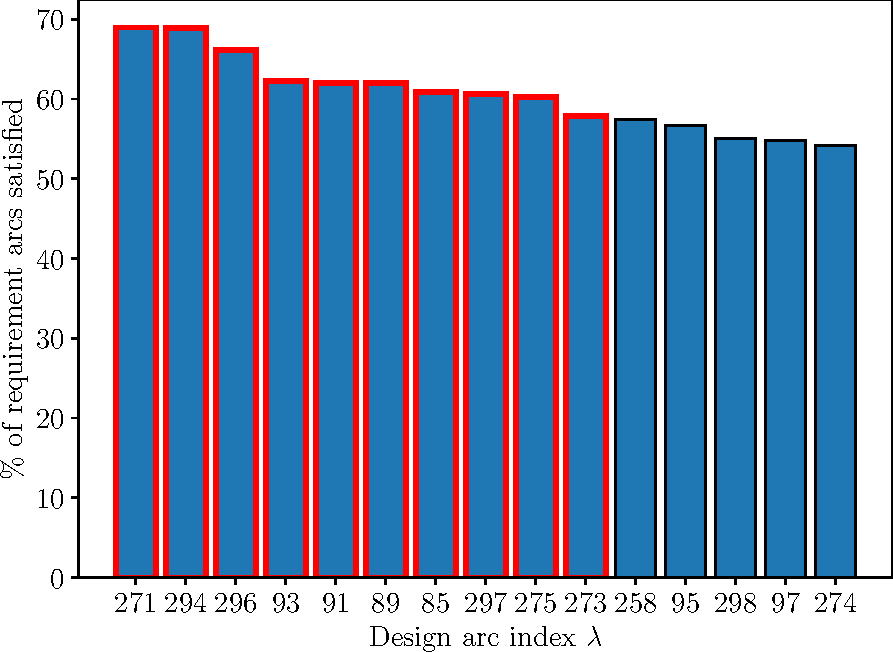
\includegraphics[width=0.45\textwidth]{12a_histogram_DOE_R}} \hspace{0.1\textwidth}%	
	\subfloat[Set of flexible design arcs \label{fig:histogramF}]{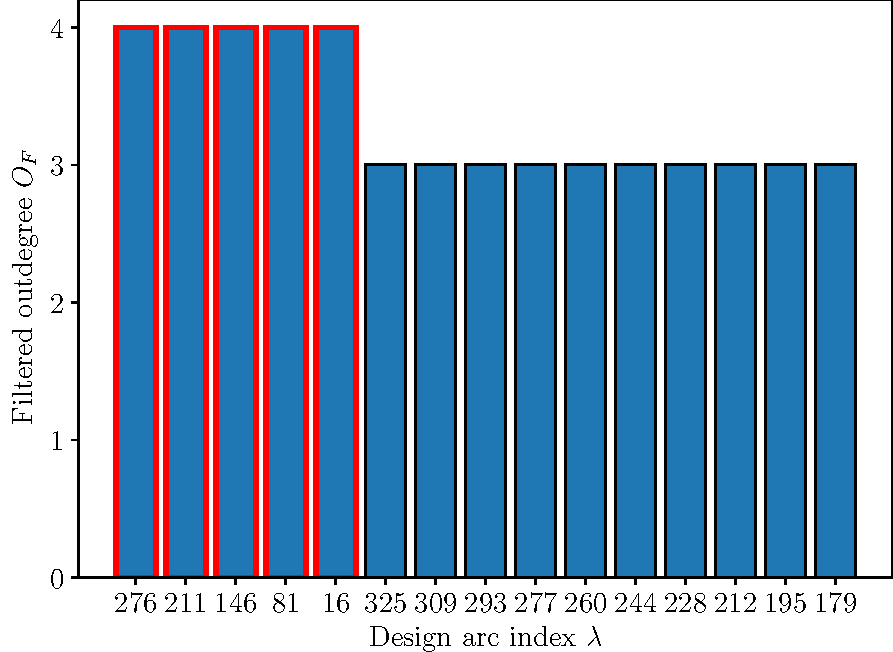
\includegraphics[width=0.45\textwidth]{12b_histogram_DOE_F}} \hspace{0.1\textwidth}%	
	\caption{Distribution of design arcs in set-based solutions}
	\label{fig:histogramplots}
\end{figure}

We highlight the top $\alpha = 10$ design arcs in Figures~\ref{fig:histogramplotsSBD} and \ref{fig:histogramplots} for visualization on a tradespace. A tradespace with the utility given by the volume of the capability set $V_c$ and weight $W$ is shown in Figure~\ref{fig:tradespaceSBD}. The Pareto front for the tradespace is obtained by solving the problem in Equation~\ref{eq:optproblembiobj}.

\begin{figure}[h!]
	\centering
	\subfloat[Set-based design arcs objective: minimize cumulative excess\label{fig:tradespaceSBDE}]{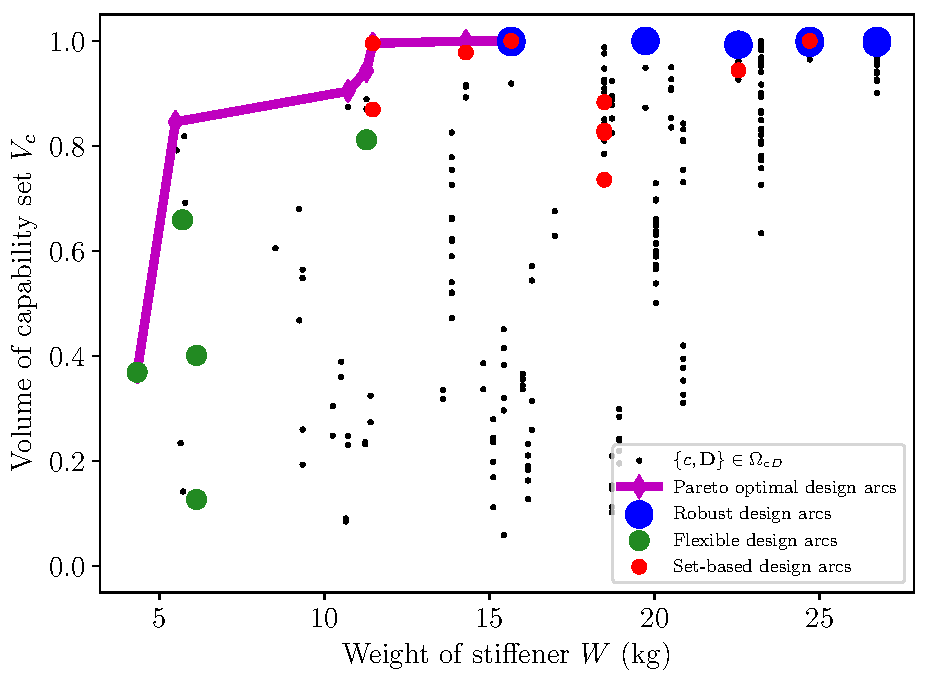
\includegraphics[width=0.45\textwidth]{13a_tradespace_pareto_E}} \hspace{0.1\textwidth}%
	\subfloat[Set-based design arcs: minimize cumulative weight\label{fig:tradespaceSBDW}]{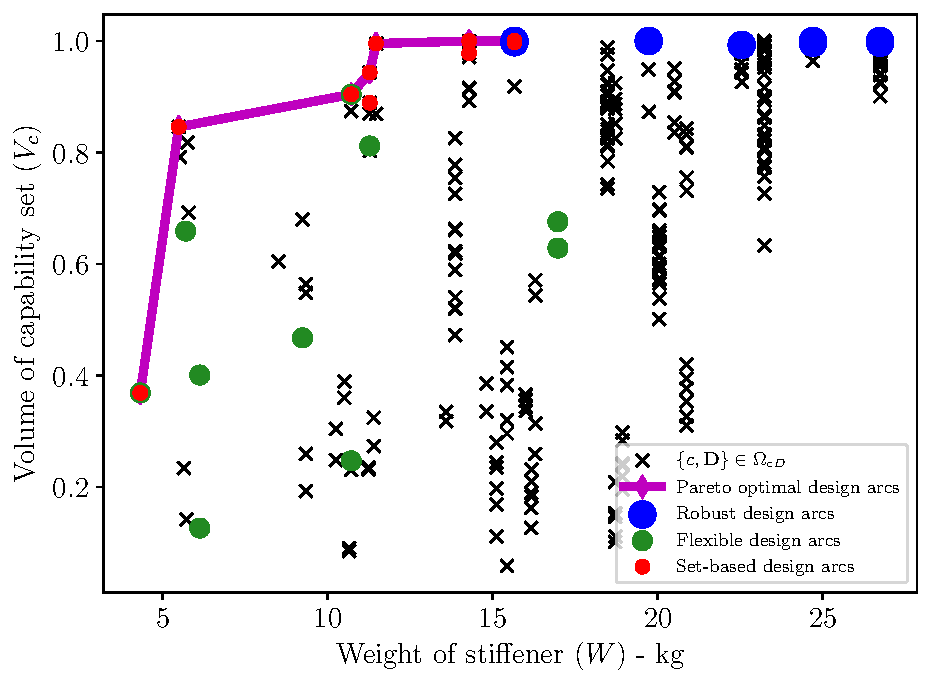
\includegraphics[width=0.45\textwidth]{13b_tradespace_pareto_W}} \hspace{0.1\textwidth}%	
	\caption{Tradespace with design arcs projected}
	\label{fig:tradespaceSBD}
\end{figure}

From the tradespace, we can draw several insights. The flexible set-based solution minimizes cost but also minimizes utility. In contrast, the robust design set maximizes utility but also maximizes the cost. The set-based solution obtained by optimization with respect to excess or weight balances utility with cost. The weight optimized set-based solution has a larger spread than the excess optimized solution. We quantify the size of the set-based solutions by their convex hulls. We use the convex hull to calculate three metrics: the area spanned by the set, location of the set given by its centroid and proximity to the Pareto front given by the distance from the centroid to the nearest Pareto point.

We report the convex hull metrics in Table~\ref{table:convexhullresults}.

\begin{table*}[h!]
	\centering
	\small\addtolength{\tabcolsep}{-2pt}
	\caption{Set-based solution comparison}
	\label{table:convexhullresults}
	\begin{tabular}{>{\arraybackslash}p{2cm}|C{1cm}C{1cm}|C{1cm}C{1cm}|C{1cm}C{1cm}|C{1cm}C{1cm}|C{1cm}C{1cm}}
		\toprule\toprule
		\multirow{2}{2cm}{\textbf{Quantity}} & \multicolumn{2}{c|}{Set of feasible} & \multicolumn{2}{c|}{Set of robust} & \multicolumn{2}{c|}{Set of flexible} & \multicolumn{2}{c|}{Set of optimal} & \multicolumn{2}{c}{Set of optimal}\\ 
		 & \multicolumn{2}{c|}{design arcs $\Omega_{cD}$} & \multicolumn{2}{c|}{design arcs $S_R$} & \multicolumn{2}{c|}{design arcs $S_F$} & \multicolumn{2}{c|}{design arcs $S_E$} & \multicolumn{2}{c}{design arcs $S_W$}\\ \hline
		%================================================================
		Coordinates & $W$ & $V_c$ & $W$ & $V_c$ & $W$ & $V_c$ & $W$ & $V_c$ & $W$ & $V_c$\\
		\hline
		Lower & 4.32 & 0.059 & 15.66 & 0.992 & 4.32 & 0.127 & 11.47 & 0.736 & 4.32 & 0.369\\
		Upper & 26.74 & 1.00 &  26.74 & 1.00 & 16.97 & 0.904 & 24.70 & 1.00 & 15.66 & 1.00\\
		Set centroid & 14.02 & 0.533 & 22.34 & 0.998 & 10.22 & 0.516 & 16.35 & 0.920 & 11.15 & 0.868 \\ \hline
		%================================================================
		$V_{\textrm{hyper-rectangle}}$ & \multicolumn{2}{c}{1} & \multicolumn{2}{c}{0.0038} & \multicolumn{2}{c}{0.466} & \multicolumn{2}{c}{0.166} & \multicolumn{2}{c}{0.339}\\
		$V_{\textrm{convhull}}$ & \multicolumn{2}{c}{0.758} & \multicolumn{2}{c}{0.0026} & \multicolumn{2}{c}{0.245} & \multicolumn{2}{c}{0.104} & \multicolumn{2}{c}{0.126}\\
		$\%V_{\textrm{feasible}}$ & \multicolumn{2}{c}{75.8\%} & \multicolumn{2}{c}{0.26\%} & \multicolumn{2}{c}{24.5\%} & \multicolumn{2}{c}{10.4\%} & \multicolumn{2}{c}{12.6\%}\\ \hline
		%================================================================
		$D_{\textrm{Pareto}}$ & \multicolumn{2}{c}{0.421} & \multicolumn{2}{c}{0.298} & \multicolumn{2}{c}{0.306} & \multicolumn{2}{c}{0.0904} & \multicolumn{2}{c}{0.0432}\\ 
		%================================================================
		\toprule\toprule
	\end{tabular}
\end{table*}

From Table~\ref{table:convexhullresults} we can see that the set of optimal design arcs with respect to cumulative excess $S_E$ occupies $10.4\%$ of the objective space which is less than that occupied by the set of flexible design arcs $S_F$ and greater than that occupied by the set of robust design arcs $S_R$. The set of optimal design arcs with respect to cumulative weight $S_W$ occupies $12.6\%$ which is comparable to the volume of $S_E$.

Furthermore, we can see that the sets of optimal design arcs $S_E$ and $S_W$ are close to the Pareto front which is expected since these sets aim to balance robustness with flexibility which are indirectly related to capability and weight.

Although there are a lot of commonalities between sets $S_E$ and $S_W$, there are some notable differences. Set $S_E$ favors designs that have higher capability when compared to $S_W$ as given by the $V_c$ coordinate of their centroids of 0.920 and 0.868 respectively. The discrepancy between the two sets is due to the fact that weight, or in more general cases, cost does not necessarily translate to excess. For example two designs of identical weight may have different excesses due to differences in the placement of the stiffener. It is therefore important that the designers carefully select their desired metric for optimization in the problem given by Equation~(\ref{eq:TSEoptproblem}).

We aim to analyze the top 6 designs in sets $S_E$ and $S_W$ in Figure~\ref{fig:histogramplotsSBD} by using the reduced tradespace shown in Figure~\ref{fig:reducedTSE}. We also display the geometry of the deposits that belong to these designs in Tables~\ref{table:depositionsequence_SE} and \ref{table:depositionsequence_SW}.

\begin{figure}[h!]
	\centering
	\subfloat[$S_E$\label{fig:reducedTSE_SE}]{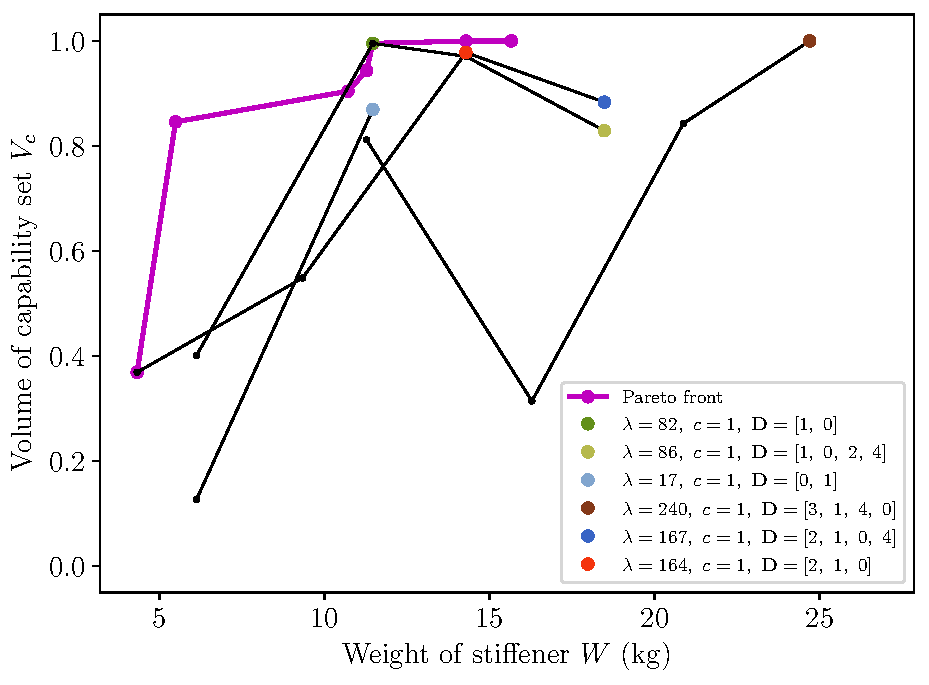
\includegraphics[width=0.5\textwidth]{14a_tradespace_pareto_E_reduced}}
	%
	\subfloat[$S_W$\label{fig:reducedTSE_SW}]{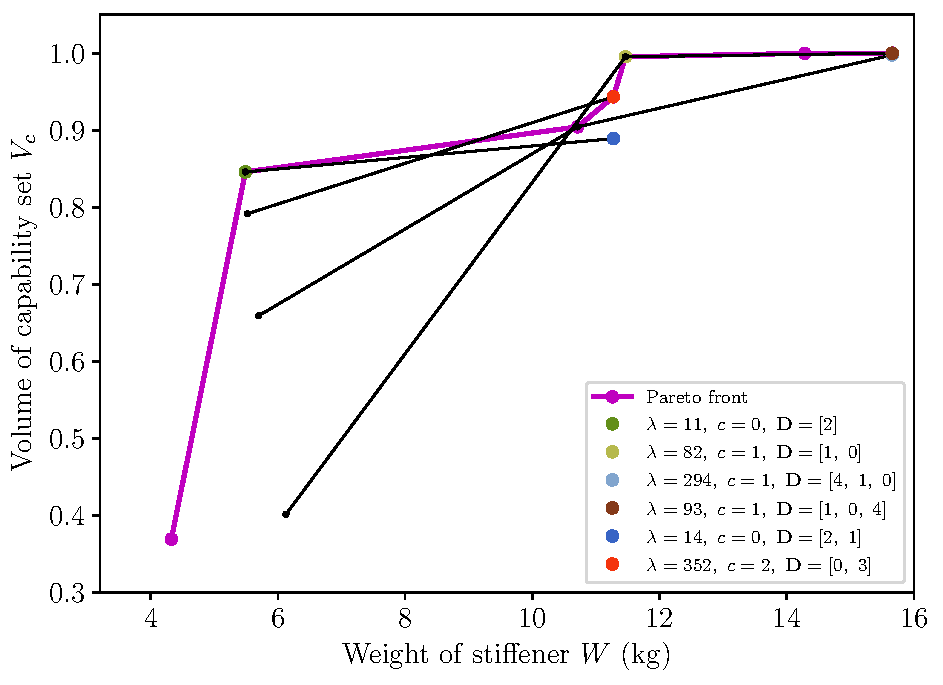
\includegraphics[width=0.5\textwidth]{15a_tradespace_pareto_W_reduced}}
	\caption{Reduced tradespace of solutions in sets $S_E$ and $S_W$}
	\label{fig:reducedTSE}
\end{figure}

Figure~\ref{fig:reducedTSE_SE} and Table~\ref{table:depositionsequence_SE} show that the top 6 designs in $S_E$ share the same concept $c=1$. The top two designs ($\lambda = 82$ and $\lambda = 86$) share the first two deposit choices $D_1=1$ and $D_2=0$. The runner-up design ($\lambda = 86$) adds two additional deposits to the top ranked design ($\lambda = 82$). From Figure~\ref{fig:reducedTSE_SE}, it can be seen that the addition of two more deposits to the top ranked design reduced the capability $V_c$. This is because of the overstiffening of the \ac{TRS} outercasing by the addition of more stiffeners. This overstiffening reduced the fatigue life of the outercasing by inducing concentrated tensile stresses in the unreinforced gaps between the stiffener deposits. The third ranked design ($\lambda = 17$) is identical in geometry to the top ranked designs as seen in Table~\ref{table:depositionsequence_SE} but has the order of the deposit choices interchanged. The discrepancy between $\lambda = 17$ and $\lambda = 82$ is due to the difference in thermomechanical effect of depositing $D_1=0$ first instead of $D_1=1$.

Similar observations can be seen for set $S_W$ in Figure~\ref{fig:reducedTSE_SW}. However, the top performing design belonged to concept $c=0$ while the 6th ranked design belonged to concept $c=2$. Furthermore, the number of deposits used for any given design arc did not exceed $o=3$. In contrast, $S_E$ featured many designs with $o=4$. The fewer number of deposits in $S_W$ can be attributed to the preference of the algorithm for minimizing weight above all. Another difference between $S_W$ and $S_E$ is that most designs in $S_W$ are Pareto optimal as given by the proximity metric in Table~\ref{table:convexhullresults}. $S_W$ has a Pareto proximity metric of $0.0432$ units which is smaller than the value of $0.0904$ units belonging to $S_E$. This is due to the reasons explained earlier regarding the discrepancy between the weight (or cost) and excess. 

% We can see that some of the top performing design arcs are sometimes children of a better performing parent design arc. This is the case with design arc $\lambda = 17$ being the parent of $\lambda = 28$ although $\lambda = 17$ is higher up the ranking within $S_E$. 

\newcommand{\resultsCW}{1.7cm}
\newcommand{\dARA}{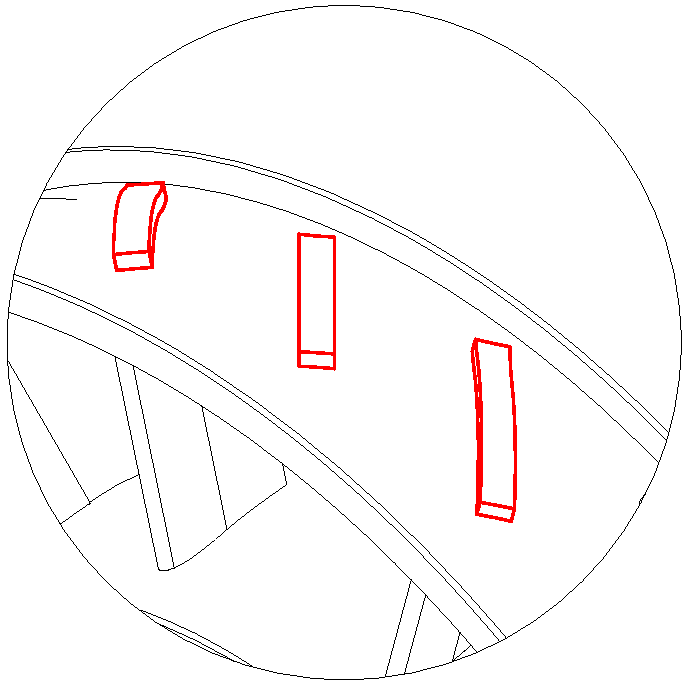
\includegraphics[height=1.7cm]{table_E_results/C1D1.pdf}}
\newcommand{\dBRA}{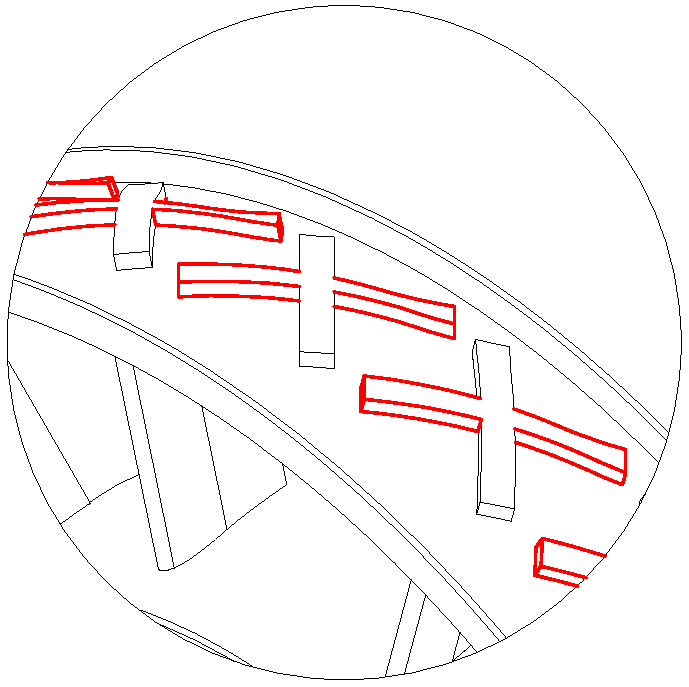
\includegraphics[height=1.7cm]{table_E_results/C1D10.pdf}}

\newcommand{\dARB}{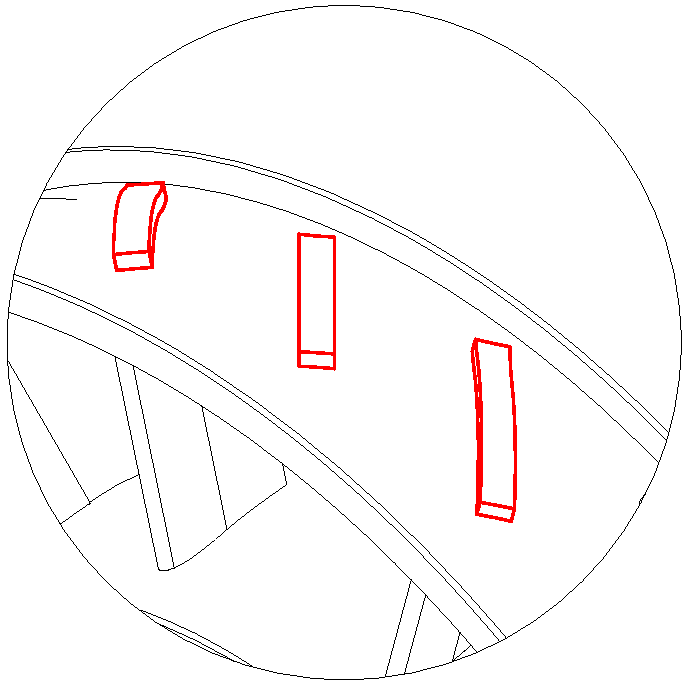
\includegraphics[height=1.7cm]{table_E_results/C1D1.pdf}}
\newcommand{\dBRB}{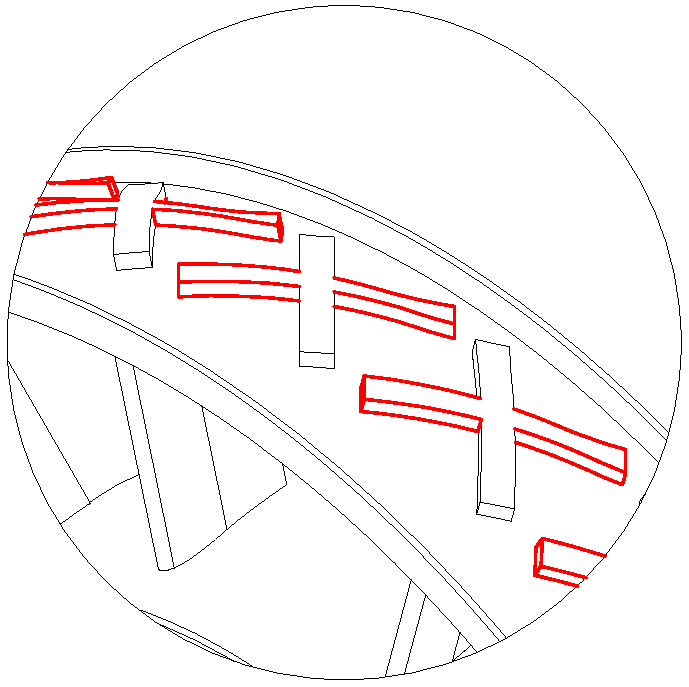
\includegraphics[height=1.7cm]{table_E_results/C1D10.pdf}}
\newcommand{\dCRB}{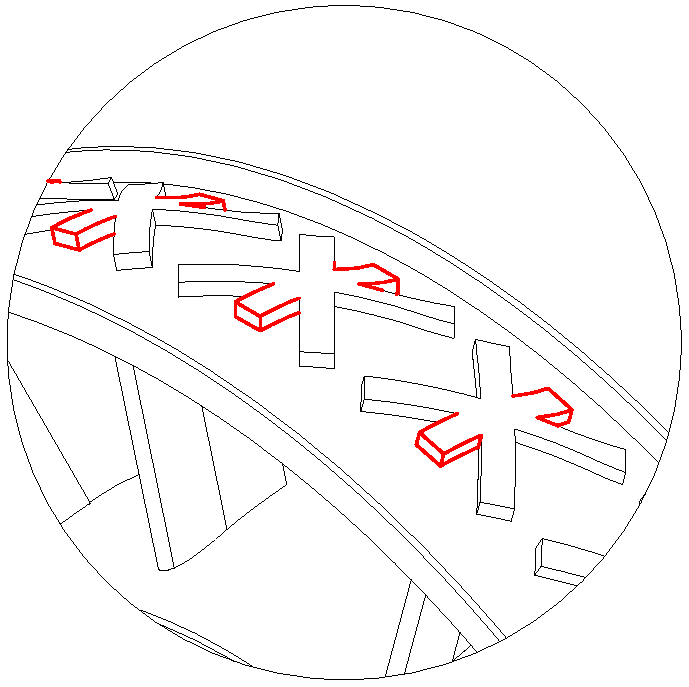
\includegraphics[height=1.7cm]{table_E_results/C1D102.pdf}}
\newcommand{\dDRB}{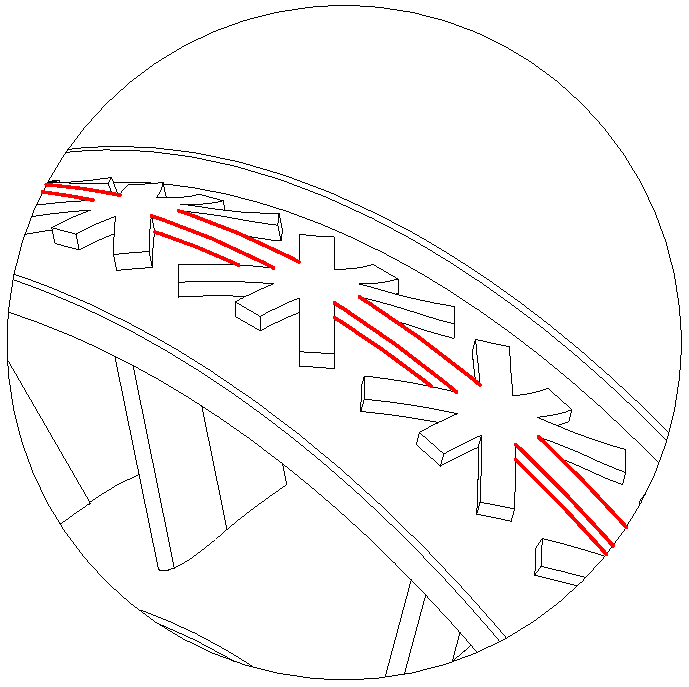
\includegraphics[height=1.7cm]{table_E_results/C1D1024.pdf}}

\newcommand{\dARC}{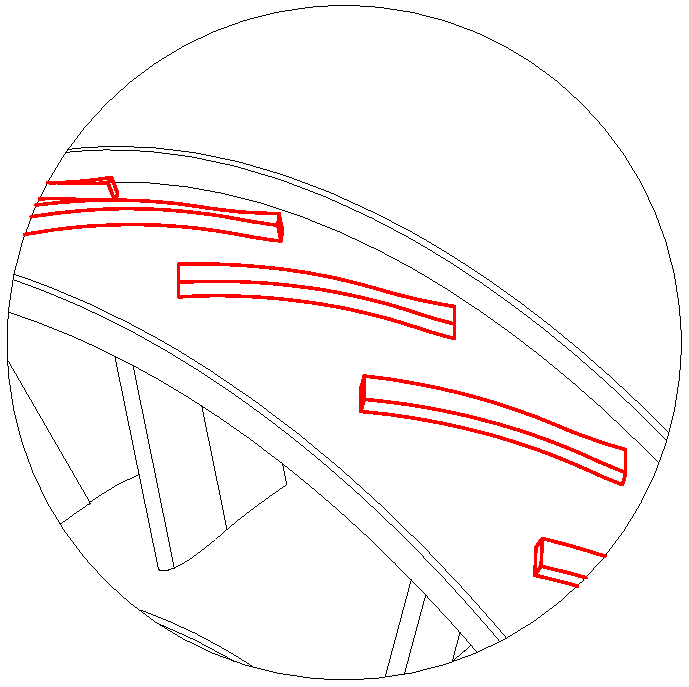
\includegraphics[height=1.7cm]{table_E_results/C1D0.pdf}}
\newcommand{\dBRC}{\includegraphics[height=1.7cm]{table_E_results/C1D01.pdf}}

\newcommand{\dARD}{\includegraphics[height=1.7cm]{table_E_results/C1D3.pdf}}
\newcommand{\dBRD}{\includegraphics[height=1.7cm]{table_E_results/C1D31.pdf}}
\newcommand{\dCRD}{\includegraphics[height=1.7cm]{table_E_results/C1D314.pdf}}
\newcommand{\dDRD}{\includegraphics[height=1.7cm]{table_E_results/C1D3140.pdf}}

\newcommand{\dARE}{\includegraphics[height=1.7cm]{table_E_results/C1D2.pdf}}
\newcommand{\dBRE}{\includegraphics[height=1.7cm]{table_E_results/C1D21.pdf}}
\newcommand{\dCRE}{\includegraphics[height=1.7cm]{table_E_results/C1D210.pdf}}
\newcommand{\dDRE}{\includegraphics[height=1.7cm]{table_E_results/C1D2104.pdf}}

\newcommand{\dARF}{\includegraphics[height=1.7cm]{table_E_results/C1D2.pdf}}
\newcommand{\dBRF}{\includegraphics[height=1.7cm]{table_E_results/C1D21.pdf}}
\newcommand{\dCRF}{\includegraphics[height=1.7cm]{table_E_results/C1D210.pdf}}

\begin{table}[h!]
	\centering
	\renewcommand{\arraystretch}{1.0}% Wider
	\footnotesize\addtolength{\tabcolsep}{-5pt}
	\caption{Top performing design arcs in $S_E$ detailed annotation}
	\label{table:depositionsequence_SE}
	\begin{tabular}{>{\centering\arraybackslash}m{\resultsCW}>{\centering\arraybackslash}m{\resultsCW}>{\centering\arraybackslash}m{\resultsCW}>{\centering\arraybackslash}m{\resultsCW}>{\centering\arraybackslash}m{\resultsCW}>{\centering\arraybackslash}m{\resultsCW}>{\centering\arraybackslash}m{\resultsCW}}
	\hline\hline

	\bf Design arc Index & \bf concept & \bf 1st deposit & \bf 2nd deposit & \bf 3rd deposit & \bf 4th deposit & \bf 5th deposit \\
	$\lambda$ & $c$ & $D_1$ & $D_2$ & $D_3$ & $D_4$ & $D_5$\\ \hline
	%================================================================
	82 & 1 & \dARA & \dBRA & & & \\ 
	86 & 1 & \dARB & \dBRB & \dCRB & \dDRB & \\
	17 & 1 & \dARC & \dBRC & & & \\ 
	240 & 1 & \dARD & \dBRD & \dCRD & \dDRD & \\ 
	167 & 1 & \dARE & \dBRE & \dCRE & \dDRE & \\
	164 & 1 & \dARF & \dBRF & \dCRF & & \\
	%================================================================
	\hline\hline
	\end{tabular}
\end{table}

\renewcommand{\resultsCW}{1.7cm}
\renewcommand{\dARA}{\includegraphics[height=1.7cm]{table_W_results/C0D2.pdf}}

\renewcommand{\dARB}{\includegraphics[height=1.7cm]{table_W_results/C1D1.pdf}}
\renewcommand{\dBRB}{\includegraphics[height=1.7cm]{table_W_results/C1D10.pdf}}

\renewcommand{\dARC}{\includegraphics[height=1.7cm]{table_W_results/C1D4.pdf}}
\renewcommand{\dBRC}{\includegraphics[height=1.7cm]{table_W_results/C1D41.pdf}}
\newcommand{\dCRC}{\includegraphics[height=1.7cm]{table_W_results/C1D410.pdf}}

\renewcommand{\dARD}{\includegraphics[height=1.7cm]{table_W_results/C1D1.pdf}}
\renewcommand{\dBRD}{\includegraphics[height=1.7cm]{table_W_results/C1D10.pdf}}
\renewcommand{\dCRD}{\includegraphics[height=1.7cm]{table_W_results/C1D104.pdf}}

\renewcommand{\dARE}{\includegraphics[height=1.7cm]{table_W_results/C1D2.pdf}}
\renewcommand{\dBRE}{\includegraphics[height=1.7cm]{table_W_results/C1D21.pdf}}

\renewcommand{\dARF}{\includegraphics[height=1.7cm]{table_W_results/C2D0.pdf}}
\renewcommand{\dBRF}{\includegraphics[height=1.7cm]{table_W_results/C2D03.pdf}}

\begin{table}[h!]
	\centering
	\renewcommand{\arraystretch}{1.0}% Wider
	\footnotesize\addtolength{\tabcolsep}{-5pt}
	\caption{Top performing design arcs in $S_W$ detailed annotation}
	\label{table:depositionsequence_SW}
	\begin{tabular}{>{\centering\arraybackslash}m{\resultsCW}>{\centering\arraybackslash}m{\resultsCW}>{\centering\arraybackslash}m{\resultsCW}>{\centering\arraybackslash}m{\resultsCW}>{\centering\arraybackslash}m{\resultsCW}>{\centering\arraybackslash}m{\resultsCW}>{\centering\arraybackslash}m{\resultsCW}}
	\hline\hline

	\bf Design arc Index & \bf concept & \bf 1st deposit & \bf 2nd deposit & \bf 3rd deposit & \bf 4th deposit & \bf 5th deposit \\
	$\lambda$ & $c$ & $D_1$ & $D_2$ & $D_3$ & $D_4$ & $D_5$\\ \hline
	%================================================================
	11 & 0 & \dARA & & & & \\ 
	82 & 1 & \dARB & \dBRB & & & \\
	294 & 1 & \dARC & \dBRC & \dCRC & & \\ 
	93 & 1 & \dARD & \dBRD & \dCRD & & \\ 
	14 & 1 & \dARE & \dBRE & & & \\
	352 & 2 & \dARF & \dBRF & & & \\
	%================================================================
	\hline\hline
	\end{tabular}
\end{table}

\begin{figure}[h!]
	\centering
	\subfloat[$S_E$\label{fig:piechart_concept_SE}]{\includegraphics[width=0.5\textwidth]{14c_concept_pie_chart_E}} 
	%
	\subfloat[$S_W$\label{fig:piechart_concept_SW}]{\includegraphics[width=0.5\textwidth]{15c_concept_pie_chart_W}} 
	\caption{Distribution of concepts in sets $S_E$ and $S_W$}
	\label{fig:piechart_concept}
\end{figure}

We analyze the the distribution of the concept choices $c$ within the set $S_E$ in Figure~\ref{fig:piechart_concept_SE}. We can see that concept choice $c=1$ dwarfs the other two concept choices. This is because the "hatched" concept has deposit choices with relatively high capability and excess. The discontinuous stiffener design featured by its various deposits provided sufficient reinforcement without overstiffening the outercasing. This contrasts the deposit choices available to the "wavy" and "tubular" stiffener concepts which are continuous.

We also look at the distribution of concept choices $c$ within the set $S_W$ in Figure~\ref{fig:piechart_concept_SW}. Two concept choices, $c=0$ and $c=1$ are comparable in terms of frequency within the set. This is because both concepts contain deposit choices that are low in weight. Since the optimization objective for set $S_W$ is weight the low weight deposit choices within these concepts are equally preferred.

\begin{figure}[h!]
	\centering
	\subfloat[$S_E$\label{fig:piechart_D1_SE}]{\includegraphics[width=0.5\textwidth]{14b_1st_stage_pie_E}} 
	%
	\subfloat[$S_W$\label{fig:piechart_D1_SW}]{\includegraphics[width=0.5\textwidth]{15b_1st_stage_pie_W}} 
	\caption{Distribution of first deposit $D_1$ when concept $c=1$ is selected in sets $S_E$ and $S_W$}
	\label{fig:piechart_D1}
\end{figure}

We then analyze the distribution of the first choice $D_1$ in the design arcs within the set $S_E$. This distribution is shown in Figure~\ref{fig:piechart_D1_SE}. We can see from this distribution that the redesign choice $D_1 = 1$ is chosen most frequently due the high capability $V_c$ of this deposit choice and its children. The third most common design choice is $D_1 = 0$ which is comparable in frequency to $D_1 = 2$. However, it should be noted that committing to $D_1 = 0$ restricts the designers' choices later in the product's cycle. Figure~\ref{fig:reducedTSE_SE} shows that $\lambda = 17$ is the only possible design arc with $D_1 = 0$. This is in contrast to $D_1 = 1$ that can be used to obtain two different design arcs $\lambda = 82$ and $\lambda = 86$. These additional insights obtained by close examination of the tradespace can be beneficial as opposed to picking the most obvious result from Figure~\ref{fig:piechart_D1}.

The tools developed in this chapter can help designers make informed decisions about the sequence of redesign choices during a product cycle. These insights are particularly useful for determining the first redesign choice when uncertainty is high and the number of possible choices is at its maximum.

%============================== SUMMARY ================================%
\section{Summary}
\label{sec:TSEcontsummary}

This chapter presented a set-based design tool for generating optimal redesign sequences for a product as its lifecycle or development process progresses. These sequences of design choices are represented by design arcs and are obtained by solving a combinatorial optimization problem such that reliability constraints governed by the uncertain requirements are satisfied. The cost function used in optimization is based on the level of excess embedded in a design. 

We mathematically formulate a novel tool for quantifying the level of excess in a design when multiple uncertain parameters are considered simultaneously. Regions of the multi-dimensional parameter space are classified into design capability, requirements, excess or buffer by using a surrogate model. The volume of these sets is obtained via Monte Carlo integration in order to alleviate the curse of dimensionality when considering multi-dimensional problems.

By minimizing the volume of the excess set for a particular design and requirement, overdesign costs are mitigated. We vary the requirements using Monte Carlo simulation with importance sampling to generate requirement arcs. The optimization problem is solved for each requirement arc to obtain a set of corresponding design arcs. 

Tradespace exploration is used to visualize the set of optimal design arcs and compare it to sets of flexible and robust design arcs. Tradespace exploration showed that our approach results in a set of design arcs that balance flexibility and robustness. An examination of the frequency of each design choice within the set of parametric optimal design arcs provides designers with useful insights about the best approach at the early stages of the product's lifecycle or development process when uncertainty is high and decisions have a lasting impact on the product's performance for the remainder of its lifecycle.

The work in this chapter extends the approach used in Chapter~\ref{ch:scalableSBD} to include problems where multiple changes in requirements may occur. This is represented by the requirement arcs discussed in this chapter. Furthermore, robustness in addition to flexibility was quantified and used as a design metric in this chapter.

In the next chapter, we discuss emerging algorithm for obtaining sets of design solutions when uncertain parameters govern the design optimization problem. Such approaches can help address the need for extensive exploration of the parameter space or the set of possible requirements (given by $\Omega_R$) by reducing the number of needed function evaluations. We show how such approaches can substitute parts of the algorithms that have been developed in this chapter and Chapter~\ref{ch:scalableSBD}.

% Chapter 06: Stochastic optimization
%%%%%%%%%%%%%%%%%%%%%%%%%%%%%%%%%%%%%%%%%%%%%%%%%%%%%%%
%%              Stochastic optimization              %%
%%%%%%%%%%%%%%%%%%%%%%%%%%%%%%%%%%%%%%%%%%%%%%%%%%%%%%%
\chapter{Managing uncertain requirements by means of stochastic optimization}
\chaptermark{Managing uncertain requirements by means of stochastic optimization}
\label{ch:stohasticopt}
%%%%%%%%%%%%%%%%%%%%%%%%%%%%%%%%%%%%%%%%%%%%%%%%%%%%%%%

This chapter explores the use of state-of-the-art stochastic optimization algorithms for managing uncertain requirements in design problems. We show how a set of design solutions can be obtained from the models defined in Chapter~\ref{ch:thermomechanical} via a stochastic version of \ac{MADS}, \texttt{StoMADS} \cite{Audet2019}.

The method described in this chapter can help simplify the algorithms introduced in Chapters \ref{ch:scalableSBD} and \ref{ch:TSEcont} by eliminating the steps involved in searching for a set of parametric optimal solutions.

%============================ METHODOLOGY ============================%
\section{Methodology} \label{sec:STOmethods}

Consider the optimization problem defined in Section \ref{subsec:SBDparametric} in Equation~(\ref{eq:SBDoptproblem}). The objectives and constraints are a function of uncertain parameters $\mathbf{p}$. In this section we denote the uncertain parameters by random variables $\mathbf{P} = \left[P_1,P_2,\cdots,P_m\right]$ (not to be confused with the reliability vector defined in Chapter~\ref{ch:TSEcont}). The objective and constraints functions in Equation~(\ref{eq:SBDoptproblem}) are deterministic in nature. By replacing the uncertain parameters with their random counterparts, the objective and constraint functions become stochastic

\begin{equation}
	\begin{aligned}
		& \underset{\mathbf{x}}{\text{minimize}}
		& & \hat{f}(\mathbf{x})~\textrm{where}~\hat{f}(\mathbf{x})=\mathbb{E}_{\mathbf{P}}\left[\hat{f}_{\mathbf{P}}(\mathbf{x})\right]\\
		& \text{subject to}
		& & \hat{\mathbf{g}}(\mathbf{x}) \le \mathbf{0}~\textrm{where}~\hat{\mathbf{g}}(\mathbf{x})=\mathbb{E}_{\mathbf{P}}\left[\hat{\mathbf{g}}_{\mathbf{P}}(\mathbf{x})\right],
	\end{aligned}
	\label{eq:STOoptproblem}
\end{equation}

where $\mathbb{E}_{\mathbf{P}}$ denotes the expectation with respect to the vector of random variables $\mathbf{P}$. $\hat{f}_{\mathbf{P}}(\mathbf{x})$ and $\hat{\mathbf{g}}_{\mathbf{P}}(\mathbf{x})$ denote the stochastic version of the surrogate models for the engineering design problem being solved.

$\hat{f}_{\mathbf{P}}(\mathbf{x})$ and $\hat{\mathbf{g}}_{\mathbf{P}}(\mathbf{x})$ are obtained from their deterministic counterparts $\hat{f}(\mathbf{x};{\mathbf{p}})$ and $\hat{\mathbf{g}}(\mathbf{x};{\mathbf{p}})$ by randomly sampling the components of the parameter vector $\mathbf{p}$ from a joint \ac{PDF} $F_{\mathbf{X}}(\mathbf{p})$. In this chapter we use a uniform distribution for the joint \ac{PDF} although other distributions can be used depending on the problem.

The optimization problem in Equation~(\ref{eq:STOoptproblem}) is solved via \texttt{StoMADS} to obtain a set of candidate solutions for the optimizer $\mathbf{X}^*=  \{ \mathbf{x}^*_1,\mathbf{x}^*_2,\ldots,\mathbf{x}^*_w \} $.

We demonstrate the capabilities of \texttt{StoMADS} by solving a \ac{TRS} remanufacturing problem where uncertain parameters ae involved.

%========================= APPLICATION PROBLEM =======================%
\section{Application problem} \label{sec:STOcasestudy}

We investigate the deposition of a circumferential stiffener on the outer casing of a \ac{TRS} (shown in Figure~\ref{fig:TRSoverview}) subject to 4 uncertain temperature loads (shown in Figure~\ref{fig:thermalloads}). We formulate the problem as follows:

\begin{equation} \label{eq:Stoproblemdet}
    \begin{aligned}
        & \underset{\mathbf{x}}{\text{minimize}}
        & & \hat{f}(\mathbf{x};\mathbf{p}) = -\hat{n_{\textrm{safety}}}(\mathbf{x};T_1,T_2,T_3,T_4)\\
        & \text{subject to}
        & & {g_{\textrm{linear}}}(\mathbf{x}) = x_3 + x_1 - W_{\textrm{total}} \le 0\\
        & \text{where}
        & & \mathbf{x} = \left[x_1,x_2,x_3\right]^{\mathrm{T}}\\
    \end{aligned}
\end{equation}

The objective function is obtained from a surrogate model for the safety factor $\hat{n_{\textrm{safety}}}$ where the inputs are the stiffener dimensions $x_1,x_2,$ and $x_3$ and temperature loads $T_1,T_2,T_3,$ and $T_4$.

The design variables for this problem govern the circumferential stiffener geometry (given by $x_1,x_2,$ and $x_3$). The uncertain parameters for this problem are the 4 temperature loads experienced by the \ac{TRS} ($T_1,T_2,T_3,$ and $T_4$). We extract the relevant design variables and parameters from Table~\ref{table:modelinputs} and list them in the tables below:


\begin{table}[h!]
    \centering
    \renewcommand{\arraystretch}{1.0}% Wider
    \small\addtolength{\tabcolsep}{-2pt}
    \caption{Design variables ${\textbf{x}}$}
    \label{table:STOmodelinputs}
    \begin{tabular}{lcccc}
    \hline\hline
    \bf Design variable & \bf Notation & \bf Units & \bf Lower bound & \bf Upper bound \\
    \hline
    Stiffener axial position & $x_1$ & mm & 37 & 145 \\
    Stiffener thickness  & $x_2$ & mm & 2 & 10 \\
    Stiffener width & $x_3$ & mm & 10 & 40  \\
    \hline\hline
    \end{tabular}
\end{table}

\begin{table}[h!]
	\centering
	\renewcommand{\arraystretch}{1.0}% Wider
	\small\addtolength{\tabcolsep}{-2pt}
	\caption{Relevant model parameters and constants}
	\label{table:STOmodelparameters}
	\begin{tabular}{lccc}
	\hline\hline
	\bf Parameter/constant & \bf Notation & \bf Units & \bf Value \\
	\hline
    %================================================================
    \multicolumn{4}{c}{Uncertain parameters $\mathbf{p}$} \\ 
	Nacelle temperature & $T_1$ & $^{o}$C & $300 \pm 100$ \\ 
	Tailcone temperature & $T_2$ & $^{o}$C & $400 \pm 100$ \\ 
	Rotor temperature & $T_3$ & $^{o}$C & $450 \pm 100$ \\ 
	Gas surface temperature & $T_4$ & $^{o}$C & $600 \pm 100$ \\ \hline
    %================================================================
    \multicolumn{4}{c}{Constant parameters} \\
	Laser Power & ${P_\textrm{laser}}$ & W &  3806 \\ 
	Laser beam radius & ${r_l}$ & mm & 14.2 \\ 
	Scanning speed& ${V}$ & mm/s & 5.0 \\ 
	Laser penetration depth & $D_p$ & mm & 5.0 \\
	Substrate base width & $W_{\textrm{total}}$ & mm & $155$ \\
	%================================================================
	\hline\hline
	\end{tabular}
\end{table}

The design problem in Equation~(\ref{eq:Stoproblemdet}) is transformed to its stochastic counterpart by randomly sampling the uncertain parameters from a uniform distribution

\begin{equation}
	\begin{aligned}
		& \underset{\mathbf{x}}{\text{minimize}}
		& & \mathbb{E}_{\mathbf{P}}\left[\hat{f}_{\mathbf{P}}(\mathbf{x})\right]\\
		& \text{subject to}
		& & {g_{\textrm{linear}}}(\mathbf{x}) = x_3 + x_1 - W_{\textrm{total}} \le 0\\
        & \text{where}
        & & \mathbf{x} = \left[x_1,x_2,x_3\right]^{\textrm{T}}\\
        & & & \mathbf{P} = \left[T_1,T_2,T_3,T_4\right]^{\textrm{T}},\\
	\end{aligned}
	\label{eq:STOproblemsto}
\end{equation}

where $\hat{f}_{\mathbf{P}}(\mathbf{x})$ is the stochastic version of the objective and the random vector $\mathbf{P}$ has its components sampled from a uniform distribution. The constraint remains unchanged since its does not involve uncertain parameters.

Before solving the problem in Equation~(\ref{eq:STOproblemsto}), we perform Monte Carlo simulation on the stochastic objective function to determine the effect of the design variables on the expected value of the objective.

%---------------------------------------------------------------------%
% Monte Carlo simulation
\subsection{Monte Carlo simulation of stochastic objective function} \label{subsec:MCSsto}


For each design variable in $\mathbf{x}$, we vary one variable at a time while holding the others fixed at their nominal values as given by Table~\ref{table:STOmodelinputs}. The stochastic objective function is called $1000$ times for a given combination of variables while randomly sampling the design parameters in $\mathbf{P}$ from a uniform distribution. The upper and lower bound for the uniform distribution that each random parameter $P_m$ follows is given by Table~\ref{table:STOmodelparameters}.

The results of the Monte Carlo simulation are visualized in Figure~\ref{fig:MSCStoblackbox}. From these results, it can be seen that the expectation of the stochastic objective function $\mathbb{E}_{\mathbf{P}}\left[\hat{f}_{\mathbf{P}}(\mathbf{x})\right]$ as given by the mean of the 1000 samples for each run is dependant on the variables in $\mathbf{x}$. It can be seen that $\mathbb{E}_{\mathbf{P}}\left[\hat{f}_{\mathbf{P}}(\mathbf{x})\right]$ is maximized in the range $ 72.5 \le x_1 \le 100 $ and at $x_2 \approx 15$ and $x_3 \approx 87.5$.

\begin{figure}[h!]
	\centering
	\subfloat[Effect of $x1$, $x2=6$ mm, $x_3=25$ mm\label{fig:X1sweep}]{\includegraphics[width=0.9\textwidth]{PDF_nsafety_X1}} 
	
	\subfloat[Effect of $x2$, $x1=91$ mm, $x_3=25$ mm\label{fig:X2sweep}]{\includegraphics[width=0.9\textwidth]{PDF_nsafety_X2}} 
	\caption[]{Monte Carlo simulation of $\hat{f}_{\mathbf{P}}(\mathbf{x})$ using $1000$ samples}
\end{figure}

\begin{figure}[h!]
	\ContinuedFloat % split subfigure across multiple pages
	\subfloat[Effect of $x3$, $x1=91$ mm, $x_2=6$ mm\label{fig:X3sweep}]{\includegraphics[width=0.9\textwidth]{PDF_nsafety_X3}} 
	\caption[Monte Carlo simulation of $\hat{f}_{\mathbf{P}}(\mathbf{x})$ using $1000$ samples]{Monte Carlo simulation of $\hat{f}_{\mathbf{P}}(\mathbf{x})$ using $1000$ samples \emph{(cont.)}}
	\label{fig:MSCStoblackbox}
\end{figure}

We now solve the problem using \texttt{StoMADS} to obtain a set of solutions.

%---------------------------------------------------------------------%
% Monte Carlo simulation
\subsection{\texttt{StoMADS} results for stochastic optimization problem} \label{subsec:STOMADSresults}

We solved the problem in Equation~(\ref{eq:STOproblemsto}) using \texttt{StoMADS-PB} to obtain a set of solutions. This algorithm is a version of \texttt{StoMADS} where constraints are handled by the progressive barrier approach \cite{Audet2009}.

The problem is also solved using the deterministic version of the algorithm \texttt{NOMAD} in order to be used as a benchmark for the quality of the solutions obtained via \texttt{StoMADS-PB} \cite{LeDigabel2011}. 

It is recommended by the developers of \texttt{StoMADS-PB} to set the maximum number of blackbox evaluations parameter of the algorithm to \texttt{max\_bb\_eval}$ = (n+1) \times 1000$, where $n$ is the number of variables. As a result, 4000 iterations where used with \texttt{StoMADS-PB}.

The best four solutions in terms of the expectation of the objective function are listed in Table~\ref{table:StoMADSresults}. In order to compute the expectation, a Monte Carlo simulation was performed for each of the solutions obtained in Table~\ref{table:StoMADSresults}. The results of the Monte Carlo simulation are shown in Figure~\ref{fig:MCSstomadsresults}.

\begin{figure}[h!]
	\centering
	\includegraphics[width=0.9\textwidth]{PDF_nsafety_soln.pdf}
	\caption{Monte Carlo simulation results of \texttt{StoMADS-PB} and \texttt{NOMAD} solutions}
	\label{fig:MCSstomadsresults}
\end{figure}

\renewcommand{\ocwa}{1.5cm} % index column width
\renewcommand{\ocwb}{1.85cm} % decision arc column width
\renewcommand{\ocwc}{1.85cm} % objective column width
\renewcommand{\ocwd}{1.85cm} % constraints column width
\renewcommand{\ocwe}{1.85cm} % design arc column width
\newcommand{\ocwf}{1.85cm} % design arc column width
\newcommand{\ocwg}{1.85cm} % design arc column width

\begin{table}[h!]
	\centering
	\renewcommand{\arraystretch}{1.0}% Wider
	\addtolength{\tabcolsep}{-2pt}
	\caption{\ac{TRS} optimization problem results}
	\label{table:StoMADSresults}
	\begin{tabular}{>{\centering\arraybackslash}p{\ocwa}|>{\centering\arraybackslash}p{\ocwb}>{\centering\arraybackslash}p{\ocwc}>{\centering\arraybackslash}p{\ocwd}|>{\centering\arraybackslash}p{\ocwe}>{\centering\arraybackslash}p{\ocwf}|>{\centering\arraybackslash}p{\ocwg}}
	\hline\hline
	\bf Solution No. & \bf Axial Position & \bf Thickness & \bf Width & \multicolumn{2}{c|}{\bf Objective} & \bf Constraint \\ 
	 & \multirow{2}{\ocwb}{\centering $x_1$} & \multirow{2}{\ocwc}{\centering $x_2$} & \multirow{2}{\ocwd}{\centering $x_3$} & \multicolumn{2}{c|}{$\hat{f}_{\mathbf{P}}(\mathbf{x})$} & \multirow{2}{\ocwg}{\centering $g_{\mathrm{linear}}(\mathbf{x})$} \\ 
	 & & & & Expectation $\mathbb{E}_{\mathbf{P}}\left[\hat{f}_{\mathbf{P}}(\mathbf{x})\right]$ & Variance $\sigma^2$ & \\ \hline
	%================================================================
	\multicolumn{7}{c}{Algorithm: \texttt{StoMADS-PB} } \\\hline
	%================================================================
	1 & 100.0 & 14.8 & 89.4 & -6.63 & 0.417 & -11.58 \\
	%================================================================
	2 & 103.6 & 15.4 & 97.4 & -6.07 & 0.417 & -0.0004 \\
	%================================================================
	3 & 84.6 & 10.5 & 86.5 & -7.03 & 0.415 & -29.9 \\
	%================================================================
	4 & 84.8 & 15.1 & 79.4 & -7.08 & 0.447 & -36.8 \\\hline
	%================================================================
	\multicolumn{7}{c}{Algorithm: \texttt{NOMAD} } \\\hline
	%================================================================
	1 & 82.4 & 15.3 & 118.6 & -6.48 & 0.389 & -0.05 \\
	%================================================================
	\hline\hline
	\end{tabular}
\end{table}

It can be seen from Table~\ref{table:StoMADSresults} that the \texttt{StoMADS-PB} algorithm performs better than the \texttt{NOMAD} algorithm when comparing the expected value of the objective function at the optimizer. Only \texttt{StoMADS-PB} candidate solution 2 underperformed in terms of the expectation of the objective function relative to the \texttt{NOMAD} solution. Furthermore it can be seen that the constraint was inactive for the best performing candidate solution. It should also be noted that although the \texttt{NOMAD} algorithm is deterministic, running the problem with the same initial conditions and algorithm parameters will yield a variety of solutions due to the stochastic nature of the objective function.

We will now summarize the implications of this approach for obtaining set-based solutions in relation to the set-based design approaches that have been developed in this thesis.

%============================== SUMMARY ================================%
\section{Summary}
\label{sec:stohasticoptsummary}

This chapter presented an alternative strategy for solving parametric optimization problems. Rather than sampling the parameter space and solving the optimization problem for a given sample of parameter values, \texttt{StomMADS} can be used to directly obtain a set of solutions with an equivalent stochastic objective and constraint functions where the parameters are sampled from their respective random distributions.

The approach presented in this chapter can be used to improve Algorithms~\ref{algo:PODalgo} and \ref{algo:SBDOptalgo}. Solving the problem in Equation~(\ref{eq:STOoptproblem}) can substitute steps 1 through 8 in Algorithm~\ref{algo:PODalgo}. However, the solution to the problem in Equation~(\ref{eq:STOoptproblem}) only outputs the optimizer values in the design space. Corresponding parameter values cannot be obtained since they are intrinsic to the stochastic version of the objective and constraint functions. The set of optimizers and their corresponding parameter values are needed by Algorithm~\ref{algo:PODalgo} to construct a response surface in the parameter space.

However, the approach in this chapter can substitute steps 3 through 5 within Algorithm \ref{algo:SBDOptalgo} by randomly selecting requirement arcs from $\Omega_R$ in the stochastic version of the problem. The requirement arc corresponding to each solution in $S_{E}^*$ is not needed since only the frequency of the design arcs is needed to isolate the set-based solution.

The approach presented in this chapter can prove useful to designers who are accustomed to more traditional design practices involving point-based design. This is because \texttt{StoMADS} has a similar interface to most available deterministic design optimization approaches that output a single design solution.

% Chapter 07: Conclusion
%%%%%%%%%%%%%%%%%%%%%%%%%%%%%%%%%%%%%%%%%%%%%%%%%%%%%%%
%%                     Conclusion                    %%
%%%%%%%%%%%%%%%%%%%%%%%%%%%%%%%%%%%%%%%%%%%%%%%%%%%%%%%
\chapter{Conclusions}
\chaptermark{Conclusions}
\label{ch:conclusion}
%%%%%%%%%%%%%%%%%%%%%%%%%%%%%%%%%%%%%%%%%%%%%%%%%%%%%%%

This thesis presented a novel design methodology for managing problems involving changing requirements and parameters. The developed frameworks were implemented by the use of parametric design optimization to exhaustively explore multi-dimensional design and parameter space and is distinguished by the following features.

\begin{itemize}
    \item It manages an instantaneous or gradual change in design requirements.
    \item It constructs surrogate models of expensive engineering models to mitigate the computational cost of exploring the design and parameter space.
    \item It utilizes rigorous derivative-free optimization tools for exploring multi-dimensional design and parameter space without the need for gradients or their approximation.
    \item It provides sets of design solutions represented by response surfaces or convex hulls for multi-dimensional continuous or discrete design spaces respectively.
    \item Provides a mathematical formulation for qualitative design characteristics such as flexibility, scalability, and excess.
\end{itemize}

A total of four algorithms were developed, demonstrated, and applied to multiple remanufacturing design problems of a \ac{TRS} with different design variables, design space types (continuous or categorical), and varying requirements change scenarios (instantaneous or gradual). 

A method for mapping between design and parameter space using response surfaces was provided in Algorithm~\ref{algo:PODalgo}. A scalability constraint was formulated and applied to a remanufacturing design problem of a \ac{TRS} in Algorithm~\ref{algo:SODalgo}. These two algorithms are combined to identify a set of scalable optimal designs in the parameters space of a design problem when an instantaneous change in requirements occurs. Application of these algorithms to the \ac{TRS} remanufacturing problem provided a relatively small albeit varied set of scalable design solutions. This set of solutions is useful for reducing the design space to a manageable set of solutions for further development and detailed analysis.

Two additional algorithms were developed to manage a cascade of requirement chang\-es at discrete times in a product's lifecycle or development cycle. As part of Algorithm \ref{algo:SBDOptalgo}, three design metrics were quantified mathematically. They allow designers to quantify the capability, buffer, and excess embedded in a design. The mathematical formulation of these design metrics is novel and allows them to be quantified in a multi-dimensional parameters space where multiple parameters may change simultaneously. The algorithm favors designs that minimize cost or excess throughout the product's cycle. This algorithm was applied to a \ac{TRS} remanufacturing problem featuring a categorical design space governed by a finite set of possible design choices. The resulting set-based solution obtained by this algorithm was displayed on a tradespace.

The fourth and final algorithm, Algorithm~\ref{algo:SBDRobustalgo} was used to obtain robust and flexible design sets using tools and definitions from the literature that were adapted for a gradual change in requirements. The algorithm was also applied to the categorical \ac{TRS} remanufacturing problem and its resulting sets were superpositioned on the same tradespace used to visualize the set-based solution obtained by minimizing excess. The tradespace revealed that utilizing design optimization can help balance the amount of robustness and flexibility in a design, a problem which is difficult to address in the early stages of the product cycle due to the relatively high uncertainty during this time period.

Finally, we proposed some stochastic optimization tools that can be used to substitute parts of Algorithms~\ref{algo:PODalgo} and \ref{algo:SBDOptalgo} to make managing design and parameter spaces with relatively large dimensionality more tractable.

To the best of our knowledge, Algorithms~\ref{algo:SODalgo} and \ref{algo:SBDOptalgo}, their metrics, and constraints are novel and are a first attempt at a systematic approach for managing a wide range of requirement change scenarios that are frequently encountered in the industry.

\section{Recommendations for future work}
\label{sec:futurework}

In this thesis, we have developed novel systematic design approaches for managing a wide range of requirement change scenarios. However, there is considerable room for improvement. In this thesis, we considered continuous or categorical design spaces independently. A framework for solving problems involving mixed variable design spaces is needed to identify the most efficient design combinations possible. 

Although we have provided a varied set of tools for quantifying design changeability, the cost of change must be considered when implementing the change in order to satisfy the definition of changeability \cite{Lawand2019}.

Although we consider the cumulative weight as a proxy for lifecycle cost, this definition is not sufficient and more advanced lifecycle modelling tools should be used for computing cost \cite{Lawand2019}. This relates directly to the lifecycle of the component and its importance to circular economy principles. A changeability cost threshold must be observed by designers when making remanufacturing decisions \cite{Ross2008}. 

Future studies could also focus on other product recovery activities along the innermost circles of a \ac{CE} such as repair and reuse as they may preserve valuable resources more efficiently than remanufacturing. Nevertheless, these options need not be mutually exclusive.

The \acp{PDF} used to model the uncertain requirements in this thesis assume that the parameters governing them are not correlated. Such correlations can be easily modelled using a covariance matrix as part of the requirement formulation to involve more general scenarios. 

Importance sampling was used to make the management of a large number of requirement change scenarios more tractable. More advanced sampling techniques can be used to make the parametric studies used in this thesis more efficient. One such approach was demonstrated in Chapter \ref{ch:stohasticopt}.

{\color{red} The algorithms were designed to accommodate a wide range of optimization and search methods for managing different kinds of design problems. Application of the algorithms to different design problems featuring similar definitions of scalability, buffer, and excess but with different search methods used in lieu of \ac{MADS} would provide more insight on the effectiveness of \ac{MADS} within the developed framework.

The metrics developed in this thesis such as scalability could be generalized for other design problems where manufacturing constraints are not the only concern governing the scalability. The concept of the Jacobian provides a powerful tool for understanding the effect of changing parameters on design variables and could be used to cover a wide range of redesign scenarios in practice.}

Building on the methods developed in this thesis, should allow designers to make decisions in the early stages of the product's development process or lifecycle when innovation potential is at its highest.

\bibHeading{References}

\bibliographystyle{unsrtnat}
\bibliography{mcgilletd_KA}



\end{document}


 






